\documentclass{beamer}
\usepackage{ctex, hyperref}
\usepackage[T1]{fontenc}

% other packages
\usepackage{latexsym,amsmath,xcolor,multicol,booktabs,calligra}
\usepackage{graphicx,pstricks,listings,stackengine}
\usepackage{tikz}
\usepackage{braket}
\usepackage{amssymb}
\usetikzlibrary{quantikz2}

\author{姜忠伟\and 赵临风}
\institute{西北大学物理学院}
\title{量子搜索算法探索历程}
\date{\today}
\usepackage{NWU_Beamer}
\titlegraphic{\includegraphics[width=0.4\linewidth]{pic/nwu-logo.png}}

% defs
\def\cmd#1{\texttt{\color{red}\footnotesize $\backslash$#1}}
\def\env#1{\texttt{\color{blue}\footnotesize #1}}
\definecolor{deepblue}{rgb}{0,0,0.5}
\definecolor{deepred}{rgb}{0.6,0,0}
\definecolor{deepgreen}{rgb}{0,0.5,0}
\definecolor{halfgray}{gray}{0.55}

\lstset{
    basicstyle=\ttfamily\small,
    keywordstyle=\bfseries\color{deepblue},
    emphstyle=\ttfamily\color{deepred},   
    % Custom highlighting style
    stringstyle=\color{deepgreen},
    numbers=left,
    numberstyle=\small\color{halfgray},
    rulesepcolor=\color{red!20!green!20!blue!20},
    frame=shadowbox,
}


\begin{document}

\kaishu
\maketitle

\begin{frame}{目录}
    \tableofcontents[
        sectionstyle=show,
        subsectionstyle=show/shaded/hide,
        subsubsectionstyle=show/shaded/hide
    ]
\end{frame}



\section{量子计算基础}

\begin{frame}{布洛赫变换}
    由模长为一且忽略全局相位,Bloch球面表示为我们提供了一种更直观的方式来观察量子比特,即从量子比特到三维实球体的同构:
    \begin{equation*}\label{BlochSphereRepersentation}
        \begin{split}
            \mathbb{C}\mathbb{P}^{1}                                                                              & \to S^{2}                                                                            \\
            \ket{\psi} = \cos \frac{\theta}{2}\ket{0} + \mathrm{e}^{\mathrm{i}\varphi}\sin\frac{\theta}{2}\ket{1} & \mapsto \vec{n}_{\psi}=(\cos\varphi\sin\theta,\sin\varphi\sin\theta,\cos\theta)^{T}.
        \end{split}
    \end{equation*}
    这里 $\theta\in\left[0,\pi\right]$ and $\varphi\in\left[0,2\pi\right]$.
\end{frame}

\begin{frame}{SU2}
    From Lie group elements, any single-qubit unitary can be written as a product of exponentials of Pauli matrices by a global phase:
    \begin{equation}
        U = e^{i\alpha}\exp\left(-i\frac{\omega}{2}\vec{n}\cdot\vec{\sigma}\right),
    \end{equation}
    which $\vec{n}$ is the coordinates of the rotation axis on the Bloch sphere.
    From the isomorphism \ref{BlochSphereRepersentation}, we can also induce an isomorphism of operations on two spaces:
    \begin{equation}
        \begin{split}
            SU(2)/\{\pm 1\}                                             & \to SO(3)
            \\
            \exp\left(-i\frac{\omega}{2}\vec{n}\cdot\vec{\sigma}\right) & \mapsto \exp\left(\omega\vec{n}\cdot\vec{J}\right)
        \end{split}
    \end{equation}
    which $\omega\in\left[0,\pi\right]$ and $J_{j}$ are the three generators of Lie group $SO(3)$, the former refers to single-qubit gates and the latter to transformations on the Bloch sphere. For visualization and convenience, we let $R_{\vec{n}}(\omega) \coloneqq \exp\left(-i\frac{\omega}{2}\vec{n}\cdot\vec{\sigma}\right)$.
\end{frame}

\begin{frame}{}
    \begin{equation}
        \sigma_x = \begin{pmatrix} 0 & 1 \\ 1 & 0 \end{pmatrix}, \quad
        \sigma_y = \begin{pmatrix} 0 & -i \\ i & 0 \end{pmatrix}, \quad
        \sigma_z = \begin{pmatrix} 1 & 0 \\ 0 & -1 \end{pmatrix}.
    \end{equation}

    \begin{equation}
        H = \frac{1}{\sqrt{2}}\begin{pmatrix} 1 & 1 \\ 1 & -1 \end{pmatrix}, \quad
        S = \begin{pmatrix} 1 & 0 \\ 0 & i \end{pmatrix}, \quad
        T = \begin{pmatrix} 1 & 0 \\ 0 & e^{i\pi/4} \end{pmatrix}.
    \end{equation}
\end{frame}



\section{量子搜索算法}

\begin{frame}{背景}
    我们需要在包含$N=2^{n}$个元素的搜索空间$S=\{0,1\}^{n}$中搜索目标元素$T\subseteq S$,$T$包含$M$个元素。将输出的目标元素和非目标元素分别表示为两个态
    \begin{equation}
        \ket{\beta}\coloneqq\frac{1}{\sqrt{M}}\sum_{x\in T}\ket{x}
        \quad\text{and}\quad
        \ket{\alpha}\coloneqq\frac{1}{\sqrt{N-M}}\sum_{x\notin T}\ket{x}.
    \end{equation}
    考虑平凡的输入态
    \begin{equation}
        \ket{\psi}\coloneqq H^{\otimes n}\ket{0}
    \end{equation}
    这里将$\ket{0}^{\otimes n}$简写为$\ket{0}$。有性质
    \begin{equation}
        \braket{\alpha|\beta}=0
        \quad\text{and}\quad
        \ket{\psi}=\sqrt{\frac{N-M}{N}}\ket{\alpha}+\sqrt{\frac{M}{N}}\ket{\beta}.
    \end{equation}
\end{frame}

\begin{frame}{主要思路}
    \begin{columns}
        \column{0.4\textwidth}
        \begin{figure}[h]
            \centering
            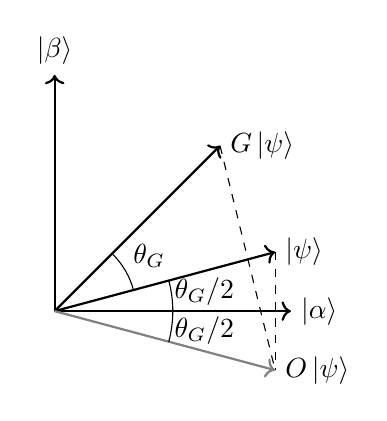
\begin{tikzpicture}
                % 绘制箭头
                \draw[->, thick] (0,0) -- (0,3) node[anchor=south] {$\ket{\beta}$};
                \draw[->, thick] (0,0) -- (2.1,2.1) node[anchor=west] {$G\ket{\psi}$};
                \draw[->, thick] (0,0) -- (2.8,0.75) node[anchor=west] {$\ket{\psi}$};
                \draw[->, thick] (0,0) -- (3,0) node[anchor=west] {$\ket{\alpha}$};
                \draw[->, gray, thick] (0,0) -- (2.8,-0.75) node[anchor=west,black] {$O\ket{\psi}$};
                % 绘制虚线
                \draw[dashed] (2.8,0.75) -- (2.8,-0.75);
                \draw[dashed] (2.1,2.1) -- (2.8,-0.75);
                % 绘制角度标记
                \draw (1.5,0) arc[start angle=0,end angle=15,radius=1.5];
                \draw (1.5,0) arc[start angle=0,end angle=-15,radius=1.5];
                \draw (1,0.27) arc[start angle=15,end angle=45,radius=1];
                % 标记角度
                \node at (1.9,0.25) {$\theta_{G}/2$};
                \node at (1.9,-0.25) {$\theta_{G}/2$};
                \node at (1.2,0.7) {$\theta_{G}$};
            \end{tikzpicture}
            \caption{Grover's算法可视化}
            \label{fig:grover}
        \end{figure}
        \column{0.6\textwidth}
        为了让初态通过不断迭代逼近目标态,我们引入两个反射操作:
        \begin{itemize}
            \item $O$ 是关于 $\ket{\alpha}$ 的反射;
            \item $D$ 是关于 $\ket{\psi}$ 的反射。
        \end{itemize}
        Grover迭代$G=DO$给了我们一个$\theta_G$的旋转, 这里$\sin(\theta_{G}/2)=\sqrt{M/N}$.
    \end{columns}
\end{frame}

\begin{frame}{主要思路}
    初始态$\ket{\psi}$通过
    \begin{equation}\label{iterations}
        R\coloneqq\left\lfloor\frac{\pi-\theta_{G}}{2\theta_{G}}\right\rceil
    \end{equation}
    次迭代可以近似得到目标态$\ket{\beta}$。\\~\\

    当 $M\ll N$,有
    \begin{equation}
        G^{R}\ket{\psi}=\cos(\frac{2R+1}{2}\theta_{G})\ket{\alpha}+\sin(\frac{2R+1}{2}\theta_{G})\ket{\beta}\approx\ket{\beta}.
    \end{equation}
\end{frame}

\begin{frame}{具体实现}{Oracle}
    由于$\ket{\alpha}$和$\ket{\beta}$是未确定的,我们需要构造一个操作对每个元素分别识别并反转
    \begin{equation}
        \begin{quantikz}
            \lstick{$\ket{x}$} & \qwbundle{n} & \gate[2][1.7cm]{U_{f}}\gateinput{$x$}\gateoutput{$x$} & \rstick{$(-1)^{f(x)}\ket{x}$} \\
            \lstick{$\ket{-}$} & & \gateinput{$y$}\gateoutput{$y\oplus f(x)$} & \rstick{$\ket{-}$}
        \end{quantikz}
    \end{equation}
    这一操作对态的影响是$\ket{x}\xrightarrow{U_{f}}(-1)^{f(x)}\ket{x}$,据此可以构造映射
    \begin{equation}
        S(x)=
        \begin{cases}
            1 & x\in T    \\
            0 & x\notin T
        \end{cases}
    \end{equation}
    \begin{equation}
        \begin{split}
            U_{S}\ket{\beta}  & =-\ket{\beta}  \\
            U_{S}\ket{\alpha} & =\ket{\alpha}.
        \end{split}
    \end{equation}
\end{frame}

\begin{frame}{具体实现}{Grover迭代}
    Then, let's construct the reflection about $\ket{\psi}$. Same as the oracle, we decompose states into
    \begin{equation}
        \ket{x}=\ket{\psi}\braket{\psi|x}+\ket{\psi_{\perp}}\braket{\psi_{\perp}|x}
    \end{equation}
    which $\ket{\psi_{\perp}}=\sqrt{\frac{M}{N}}\ket{\alpha}-\sqrt{\frac{N-M}{N}}\ket{\beta}$, and we wish
    \begin{equation}
        D\ket{x}=\ket{\psi}\braket{\psi|x}-\ket{\psi_{\perp}}\braket{\psi_{\perp}|x}.
    \end{equation}
    But this time, we know $\ket{\psi}$ specifically, operation $2\ket{\psi}\bra{\psi}-I$ is what we need. So we get the construction of the Grover iteration:
    \begin{equation}
        G=DO=(2\ket{\psi}\bra{\psi}-I)U_{S}.
    \end{equation}
\end{frame}

\begin{frame}{电路实现}
    \begin{figure}
        \centering
        \resizebox{\textwidth}{!}{
            \begin{quantikz}[column sep=0.4cm]
                \lstick{$\ket{0}$} & \qwbundle{n} & \gate{H^{\otimes n}} & \gate[2]{oracle}\gategroup[wires=2,steps=4]{Grover iteration} & \gate{H^{\otimes n}} & \gate{2\ket{0}\bra{0}-I} & \gate{H^{\otimes n}} & \gate[2]{G} & \midstick[2,brackets=none]{$\cdots$} & \gate[2]{G} & \\
                \lstick{$\ket{1}$} & & \gate{H} & & & & & & & &
            \end{quantikz}
        }
        \caption{量子搜索算法电路实现}
    \end{figure}
\end{frame}



\section{量子搜索算法的下界}

\begin{frame}{主要思路}
    在Grover算法中,Oracle是一个很特殊的操作,考虑将一部分Oracle替换成单位操作来观察Oracle带来的影响。
    \begin{equation}
        \ket{\Psi_{x}^{R}}=\prod_{j=1}^{R}U_{j}O_{x}\ket{\psi}
    \end{equation}
    \begin{equation}
        \ket{\Psi_{x}^{i,R}}=\prod_{j=i+1}^{R}U_{j}O_{x}\prod_{j=1}^{i}U_{j}I\ket{\psi}
    \end{equation}
    \begin{equation}
        \ket{\Psi^{R}}=\prod_{j=1}^{R}U_{j}I\ket{\psi}
    \end{equation}
\end{frame}

\begin{frame}{}
    考虑角度度量$A(\ket{\alpha},\ket{\beta})=\arccos\frac{\left\lvert \braket{\alpha|\beta}\right\rvert}{\left\|\ket{\alpha}\right\|\left\|\ket{\beta}\right\|}$。对我们需要的目标元素的概率有距离
    \begin{equation*}
        \begin{split}
             & \quad A(\ket{\Psi_{x}^{R}},\ket{\Psi^{R}})                                                                                                                                                                        \\
             & = \arccos\left(\left\lvert \braket{\Psi_{x}^{R}|\Psi^{R}}\right\rvert\right)                                                                                                                                      \\
             & = \arccos\left(\bra{\Psi_{x}^{R}}({\Pi}_{x}+{\Pi}_{x}^{\perp})^{\dagger}({\Pi}_{x}+{\Pi}_{x}^{\perp})\ket{\Psi^{R}}\right)                                                                                        \\
             & = \arccos\left(\left\|{\Pi}_{x}\ket{\Psi_{x}^{R}}\right\|\cdot\left\|{\Pi}_{x}\ket{\Psi^{R}}\right\|+\left\|{\Pi}_{x}^{\perp}\ket{\Psi_{x}^{R}}\right\|\cdot\left\|{\Pi}_{x}^{\perp}\ket{\Psi^{R}}\right\|\right) \\
             & = \arccos\left(\sin\phi_{x}^{R}\sin\theta_{x}^{R}+\cos\phi_{x}^{R}\cos\theta_{x}^{R}\right)                                                                                                                       \\
             & = \phi_{x}^{R}-\theta_{x}^{R} \geq \arcsin\sqrt{p}-\theta_{x}^{R}
        \end{split}
    \end{equation*}
    可以计算
    \begin{equation*}
        \frac{1}{N}\sum_{x=1}^{N}A(\ket{\Psi_{x}^{R}},\ket{\Psi^{R}})
        \geq \arcsin\sqrt{p}-\frac{1}{N}\sum_{x=1}^{N}\theta_{x}^{R}
        \geq \arcsin\sqrt{p}-\arcsin\frac{1}{\sqrt{N}}
    \end{equation*}
\end{frame}

\begin{frame}{}
    考虑$R$次迭代有距离
    \begin{equation*}
        \begin{split}
             & \quad\frac{1}{N}\sum_{x=1}^{N}{A}(\ket{\Psi_{x}^{R}},\ket{\Psi^{R}})                          \\
             & = \frac{1}{N}\sum_{x=1}^{N}{A}(\ket{\Psi_{x}^{0,R}},\ket{\Psi_{x}^{R,R}})
            \leq \frac{1}{N}\sum_{x=1}^{N}\sum_{i=1}^{R}{A}(\ket{\Psi_{x}^{i-1,R}},\ket{\Psi_{x}^{i,R}})     \\
             & = \frac{1}{N}\sum_{i=1}^{R}\sum_{x=1}^{N}{A}(O_{x}\ket{\Psi^{i}},\ket{\Psi^{i}})
            = \frac{1}{N}\sum_{i=1}^{R}\sum_{x=1}^{N}{\arccos(\left\lvert\cos(2\theta_{x}^{i})\right\rvert)} \\
             & \leq 2\sum_{i=1}^{R}{\arcsin(\frac{1}{\sqrt{N}})} = 2R{arcsin(\frac{1}{\sqrt{N}})},
        \end{split}
    \end{equation*}
    可以看到Oracle带来的距离至多是线性增加的
\end{frame}

\begin{frame}{}
    \begin{equation}
        \frac{1}{N}\sum_{x=1}^{N}A(\ket{\Psi_{x}^{R}},\ket{\Psi^{R}})\geq \arcsin\sqrt{p}-\arcsin\frac{1}{\sqrt{N}}.
    \end{equation}
    \begin{equation}
        \frac{1}{N}\sum_{x=1}^{N}{A}(\ket{\Psi_{x}^{R}},\ket{\Psi^{R}})\leq 2R{\arcsin(\frac{1}{\sqrt{N}})}.
    \end{equation}
    \begin{equation}
        R \geq\frac{\arcsin\sqrt{p}-\arcsin\frac{1}{\sqrt{N}}}{2\arcsin\frac{1}{\sqrt{N}}}.
    \end{equation}
\end{frame}



\section{龙算法}

\begin{frame}{主要思路}
    有时我们需要更精确的达到目标态。考虑经典Grover算法中没利用的相对相位,拓展Grover迭代
    \begin{equation}
        G=DO=(I-2\ket{\psi_{\perp}}\bra{\psi_{\perp}})(I-2\ket{\beta}\bra{\beta})
    \end{equation}
    至
    \begin{equation*}
        \begin{split}
            I_{D} & = I+(e^{-i\phi}-1)\ket{\psi_{\perp}}\bra{\psi_{\perp}} = e^{-i\phi}(I+(e^{i\phi}-1)\ket{\psi}\bra{\psi})                   \\
            I_{O} & = I+(e^{i\phi}-1)\ket{\beta}\bra{\beta}                                                                                    \\
            Q     & = I_{D}I_{O} = e^{-i\phi}H^{\otimes n}(I+(e^{i\phi}-1)\ket{0}\bra{0})H^{\otimes n}(I+(e^{i\phi}-1)\ket{\beta}\bra{\beta}).
        \end{split}
    \end{equation*}
\end{frame}

\begin{frame}{主要思路}
    \begin{columns}
        \column{0.5\textwidth}
        \begin{figure}[h]
            \centering
            \resizebox{\textwidth}{!}{%% Creator: Matplotlib, PGF backend
%%
%% To include the figure in your LaTeX document, write
%%   \input{<filename>.pgf}
%%
%% Make sure the required packages are loaded in your preamble
%%   \usepackage{pgf}
%%
%% Also ensure that all the required font packages are loaded; for instance,
%% the lmodern package is sometimes necessary when using math font.
%%   \usepackage{lmodern}
%%
%% Figures using additional raster images can only be included by \input if
%% they are in the same directory as the main LaTeX file. For loading figures
%% from other directories you can use the `import` package
%%   \usepackage{import}
%%
%% and then include the figures with
%%   \import{<path to file>}{<filename>.pgf}
%%
%% Matplotlib used the following preamble
%%   \def\mathdefault#1{#1}
%%   \everymath=\expandafter{\the\everymath\displaystyle}
%%   
%%   \ifdefined\pdftexversion\else  % non-pdftex case.
%%     \usepackage{fontspec}
%%   \fi
%%   \makeatletter\@ifpackageloaded{underscore}{}{\usepackage[strings]{underscore}}\makeatother
%%
\begingroup%
\makeatletter%
\begin{pgfpicture}%
\pgfpathrectangle{\pgfpointorigin}{\pgfqpoint{5.000000in}{5.000000in}}%
\pgfusepath{use as bounding box, clip}%
\begin{pgfscope}%
\pgfsetbuttcap%
\pgfsetmiterjoin%
\definecolor{currentfill}{rgb}{1.000000,1.000000,1.000000}%
\pgfsetfillcolor{currentfill}%
\pgfsetlinewidth{0.000000pt}%
\definecolor{currentstroke}{rgb}{1.000000,1.000000,1.000000}%
\pgfsetstrokecolor{currentstroke}%
\pgfsetdash{}{0pt}%
\pgfpathmoveto{\pgfqpoint{0.000000in}{0.000000in}}%
\pgfpathlineto{\pgfqpoint{5.000000in}{0.000000in}}%
\pgfpathlineto{\pgfqpoint{5.000000in}{5.000000in}}%
\pgfpathlineto{\pgfqpoint{0.000000in}{5.000000in}}%
\pgfpathlineto{\pgfqpoint{0.000000in}{0.000000in}}%
\pgfpathclose%
\pgfusepath{fill}%
\end{pgfscope}%
\begin{pgfscope}%
\pgfsetbuttcap%
\pgfsetmiterjoin%
\definecolor{currentfill}{rgb}{1.000000,1.000000,1.000000}%
\pgfsetfillcolor{currentfill}%
\pgfsetlinewidth{0.000000pt}%
\definecolor{currentstroke}{rgb}{0.000000,0.000000,0.000000}%
\pgfsetstrokecolor{currentstroke}%
\pgfsetstrokeopacity{0.000000}%
\pgfsetdash{}{0pt}%
\pgfpathmoveto{\pgfqpoint{0.000000in}{0.000000in}}%
\pgfpathlineto{\pgfqpoint{5.000000in}{0.000000in}}%
\pgfpathlineto{\pgfqpoint{5.000000in}{5.000000in}}%
\pgfpathlineto{\pgfqpoint{0.000000in}{5.000000in}}%
\pgfpathlineto{\pgfqpoint{0.000000in}{0.000000in}}%
\pgfpathclose%
\pgfusepath{fill}%
\end{pgfscope}%
\begin{pgfscope}%
\pgfpathrectangle{\pgfqpoint{0.000000in}{0.000000in}}{\pgfqpoint{5.000000in}{5.000000in}}%
\pgfusepath{clip}%
\pgfsetrectcap%
\pgfsetroundjoin%
\pgfsetlinewidth{1.003750pt}%
\definecolor{currentstroke}{rgb}{0.501961,0.501961,0.501961}%
\pgfsetstrokecolor{currentstroke}%
\pgfsetdash{}{0pt}%
\pgfpathmoveto{\pgfqpoint{0.523267in}{2.537256in}}%
\pgfpathlineto{\pgfqpoint{4.679616in}{2.598883in}}%
\pgfusepath{stroke}%
\end{pgfscope}%
\begin{pgfscope}%
\pgfpathrectangle{\pgfqpoint{0.000000in}{0.000000in}}{\pgfqpoint{5.000000in}{5.000000in}}%
\pgfusepath{clip}%
\pgfsetrectcap%
\pgfsetroundjoin%
\pgfsetlinewidth{1.003750pt}%
\definecolor{currentstroke}{rgb}{0.501961,0.501961,0.501961}%
\pgfsetstrokecolor{currentstroke}%
\pgfsetdash{}{0pt}%
\pgfpathmoveto{\pgfqpoint{2.089278in}{2.724532in}}%
\pgfpathlineto{\pgfqpoint{2.977727in}{2.432962in}}%
\pgfusepath{stroke}%
\end{pgfscope}%
\begin{pgfscope}%
\pgfpathrectangle{\pgfqpoint{0.000000in}{0.000000in}}{\pgfqpoint{5.000000in}{5.000000in}}%
\pgfusepath{clip}%
\pgfsetrectcap%
\pgfsetroundjoin%
\pgfsetlinewidth{1.003750pt}%
\definecolor{currentstroke}{rgb}{0.501961,0.501961,0.501961}%
\pgfsetstrokecolor{currentstroke}%
\pgfsetdash{}{0pt}%
\pgfpathmoveto{\pgfqpoint{2.567568in}{0.437024in}}%
\pgfpathlineto{\pgfqpoint{2.567568in}{4.674879in}}%
\pgfusepath{stroke}%
\end{pgfscope}%
\begin{pgfscope}%
\pgfpathrectangle{\pgfqpoint{0.000000in}{0.000000in}}{\pgfqpoint{5.000000in}{5.000000in}}%
\pgfusepath{clip}%
\pgfsetrectcap%
\pgfsetroundjoin%
\pgfsetlinewidth{1.003750pt}%
\definecolor{currentstroke}{rgb}{0.501961,0.501961,0.501961}%
\pgfsetstrokecolor{currentstroke}%
\pgfsetdash{}{0pt}%
\pgfpathmoveto{\pgfqpoint{4.679616in}{2.598883in}}%
\pgfpathlineto{\pgfqpoint{4.698163in}{2.579264in}}%
\pgfpathlineto{\pgfqpoint{4.680027in}{2.559845in}}%
\pgfpathlineto{\pgfqpoint{4.626621in}{2.540947in}}%
\pgfpathlineto{\pgfqpoint{4.539866in}{2.522865in}}%
\pgfpathlineto{\pgfqpoint{4.422100in}{2.505863in}}%
\pgfpathlineto{\pgfqpoint{4.275988in}{2.490175in}}%
\pgfpathlineto{\pgfqpoint{4.104448in}{2.476004in}}%
\pgfpathlineto{\pgfqpoint{3.910581in}{2.463521in}}%
\pgfpathlineto{\pgfqpoint{3.697623in}{2.452871in}}%
\pgfpathlineto{\pgfqpoint{3.468900in}{2.444171in}}%
\pgfpathlineto{\pgfqpoint{3.227794in}{2.437512in}}%
\pgfpathlineto{\pgfqpoint{2.977727in}{2.432962in}}%
\pgfpathlineto{\pgfqpoint{2.722137in}{2.430566in}}%
\pgfpathlineto{\pgfqpoint{2.464475in}{2.430348in}}%
\pgfpathlineto{\pgfqpoint{2.208195in}{2.432310in}}%
\pgfpathlineto{\pgfqpoint{1.956747in}{2.436432in}}%
\pgfpathlineto{\pgfqpoint{1.713575in}{2.442673in}}%
\pgfpathlineto{\pgfqpoint{1.482103in}{2.450972in}}%
\pgfpathlineto{\pgfqpoint{1.265724in}{2.461240in}}%
\pgfpathlineto{\pgfqpoint{1.067777in}{2.473367in}}%
\pgfpathlineto{\pgfqpoint{0.891517in}{2.487214in}}%
\pgfpathlineto{\pgfqpoint{0.740080in}{2.502614in}}%
\pgfpathlineto{\pgfqpoint{0.616422in}{2.519370in}}%
\pgfpathlineto{\pgfqpoint{0.523267in}{2.537256in}}%
\pgfusepath{stroke}%
\end{pgfscope}%
\begin{pgfscope}%
\pgfpathrectangle{\pgfqpoint{0.000000in}{0.000000in}}{\pgfqpoint{5.000000in}{5.000000in}}%
\pgfusepath{clip}%
\pgfsetrectcap%
\pgfsetroundjoin%
\pgfsetlinewidth{1.003750pt}%
\definecolor{currentstroke}{rgb}{0.501961,0.501961,0.501961}%
\pgfsetstrokecolor{currentstroke}%
\pgfsetdash{}{0pt}%
\pgfpathmoveto{\pgfqpoint{2.977727in}{2.432962in}}%
\pgfpathlineto{\pgfqpoint{2.974195in}{2.690976in}}%
\pgfpathlineto{\pgfqpoint{2.964191in}{2.947313in}}%
\pgfpathlineto{\pgfqpoint{2.947826in}{3.198502in}}%
\pgfpathlineto{\pgfqpoint{2.925279in}{3.441083in}}%
\pgfpathlineto{\pgfqpoint{2.896794in}{3.671618in}}%
\pgfpathlineto{\pgfqpoint{2.862688in}{3.886708in}}%
\pgfpathlineto{\pgfqpoint{2.823351in}{4.083013in}}%
\pgfpathlineto{\pgfqpoint{2.779252in}{4.257284in}}%
\pgfpathlineto{\pgfqpoint{2.730943in}{4.406405in}}%
\pgfpathlineto{\pgfqpoint{2.679062in}{4.527446in}}%
\pgfpathlineto{\pgfqpoint{2.624333in}{4.617724in}}%
\pgfpathlineto{\pgfqpoint{2.567568in}{4.674879in}}%
\pgfpathlineto{\pgfqpoint{2.509661in}{4.696961in}}%
\pgfpathlineto{\pgfqpoint{2.451582in}{4.682520in}}%
\pgfpathlineto{\pgfqpoint{2.394364in}{4.630699in}}%
\pgfpathlineto{\pgfqpoint{2.339086in}{4.541329in}}%
\pgfpathlineto{\pgfqpoint{2.286847in}{4.415010in}}%
\pgfpathlineto{\pgfqpoint{2.238745in}{4.253177in}}%
\pgfpathlineto{\pgfqpoint{2.195838in}{4.058138in}}%
\pgfpathlineto{\pgfqpoint{2.159114in}{3.833086in}}%
\pgfpathlineto{\pgfqpoint{2.129451in}{3.582064in}}%
\pgfpathlineto{\pgfqpoint{2.107584in}{3.309891in}}%
\pgfpathlineto{\pgfqpoint{2.094073in}{3.022051in}}%
\pgfpathlineto{\pgfqpoint{2.089278in}{2.724532in}}%
\pgfusepath{stroke}%
\end{pgfscope}%
\begin{pgfscope}%
\pgfpathrectangle{\pgfqpoint{0.000000in}{0.000000in}}{\pgfqpoint{5.000000in}{5.000000in}}%
\pgfusepath{clip}%
\pgfsetrectcap%
\pgfsetroundjoin%
\pgfsetlinewidth{1.505625pt}%
\definecolor{currentstroke}{rgb}{0.000000,0.500000,0.000000}%
\pgfsetstrokecolor{currentstroke}%
\pgfsetstrokeopacity{0.300000}%
\pgfsetdash{}{0pt}%
\pgfpathmoveto{\pgfqpoint{2.567568in}{4.150208in}}%
\pgfpathlineto{\pgfqpoint{2.261188in}{4.334955in}}%
\pgfusepath{stroke}%
\end{pgfscope}%
\begin{pgfscope}%
\pgfpathrectangle{\pgfqpoint{0.000000in}{0.000000in}}{\pgfqpoint{5.000000in}{5.000000in}}%
\pgfusepath{clip}%
\pgfsetrectcap%
\pgfsetroundjoin%
\pgfsetlinewidth{1.505625pt}%
\definecolor{currentstroke}{rgb}{0.000000,0.500000,0.000000}%
\pgfsetstrokecolor{currentstroke}%
\pgfsetstrokeopacity{0.300000}%
\pgfsetdash{}{0pt}%
\pgfpathmoveto{\pgfqpoint{2.567568in}{4.150208in}}%
\pgfpathlineto{\pgfqpoint{3.860818in}{4.090332in}}%
\pgfusepath{stroke}%
\end{pgfscope}%
\begin{pgfscope}%
\pgfpathrectangle{\pgfqpoint{0.000000in}{0.000000in}}{\pgfqpoint{5.000000in}{5.000000in}}%
\pgfusepath{clip}%
\pgfsetrectcap%
\pgfsetroundjoin%
\pgfsetlinewidth{1.505625pt}%
\definecolor{currentstroke}{rgb}{0.000000,0.000000,1.000000}%
\pgfsetstrokecolor{currentstroke}%
\pgfsetstrokeopacity{0.300000}%
\pgfsetdash{}{0pt}%
\pgfpathmoveto{\pgfqpoint{2.469199in}{3.135018in}}%
\pgfpathlineto{\pgfqpoint{3.860818in}{4.090332in}}%
\pgfusepath{stroke}%
\end{pgfscope}%
\begin{pgfscope}%
\pgfpathrectangle{\pgfqpoint{0.000000in}{0.000000in}}{\pgfqpoint{5.000000in}{5.000000in}}%
\pgfusepath{clip}%
\pgfsetrectcap%
\pgfsetroundjoin%
\pgfsetlinewidth{1.505625pt}%
\definecolor{currentstroke}{rgb}{0.000000,0.000000,1.000000}%
\pgfsetstrokecolor{currentstroke}%
\pgfsetstrokeopacity{0.300000}%
\pgfsetdash{}{0pt}%
\pgfpathmoveto{\pgfqpoint{2.469199in}{3.135018in}}%
\pgfpathlineto{\pgfqpoint{2.928500in}{1.957248in}}%
\pgfusepath{stroke}%
\end{pgfscope}%
\begin{pgfscope}%
\pgfpathrectangle{\pgfqpoint{0.000000in}{0.000000in}}{\pgfqpoint{5.000000in}{5.000000in}}%
\pgfusepath{clip}%
\pgfsetrectcap%
\pgfsetroundjoin%
\pgfsetlinewidth{1.505625pt}%
\definecolor{currentstroke}{rgb}{1.000000,0.000000,0.000000}%
\pgfsetstrokecolor{currentstroke}%
\pgfsetstrokeopacity{0.300000}%
\pgfsetdash{}{0pt}%
\pgfpathmoveto{\pgfqpoint{2.261188in}{4.334955in}}%
\pgfpathlineto{\pgfqpoint{2.205308in}{2.505905in}}%
\pgfusepath{stroke}%
\end{pgfscope}%
\begin{pgfscope}%
\pgfpathrectangle{\pgfqpoint{0.000000in}{0.000000in}}{\pgfqpoint{5.000000in}{5.000000in}}%
\pgfusepath{clip}%
\pgfsetrectcap%
\pgfsetroundjoin%
\pgfsetlinewidth{1.505625pt}%
\definecolor{currentstroke}{rgb}{1.000000,0.000000,0.000000}%
\pgfsetstrokecolor{currentstroke}%
\pgfsetstrokeopacity{0.300000}%
\pgfsetdash{}{0pt}%
\pgfpathmoveto{\pgfqpoint{2.928500in}{1.957248in}}%
\pgfpathlineto{\pgfqpoint{2.205308in}{2.505905in}}%
\pgfusepath{stroke}%
\end{pgfscope}%
\begin{pgfscope}%
\pgfpathrectangle{\pgfqpoint{0.000000in}{0.000000in}}{\pgfqpoint{5.000000in}{5.000000in}}%
\pgfusepath{clip}%
\pgfsetrectcap%
\pgfsetroundjoin%
\pgfsetlinewidth{1.505625pt}%
\definecolor{currentstroke}{rgb}{1.000000,0.000000,0.000000}%
\pgfsetstrokecolor{currentstroke}%
\pgfsetstrokeopacity{0.300000}%
\pgfsetdash{}{0pt}%
\pgfpathmoveto{\pgfqpoint{2.567568in}{0.437024in}}%
\pgfpathlineto{\pgfqpoint{2.205308in}{2.505905in}}%
\pgfusepath{stroke}%
\end{pgfscope}%
\begin{pgfscope}%
\pgfpathrectangle{\pgfqpoint{0.000000in}{0.000000in}}{\pgfqpoint{5.000000in}{5.000000in}}%
\pgfusepath{clip}%
\pgfsetrectcap%
\pgfsetroundjoin%
\pgfsetlinewidth{1.003750pt}%
\definecolor{currentstroke}{rgb}{0.501961,0.501961,0.501961}%
\pgfsetstrokecolor{currentstroke}%
\pgfsetdash{}{0pt}%
\pgfpathmoveto{\pgfqpoint{0.523267in}{2.537256in}}%
\pgfpathlineto{\pgfqpoint{0.463022in}{2.556014in}}%
\pgfpathlineto{\pgfqpoint{0.437702in}{2.575354in}}%
\pgfpathlineto{\pgfqpoint{0.448827in}{2.594960in}}%
\pgfpathlineto{\pgfqpoint{0.497333in}{2.614490in}}%
\pgfpathlineto{\pgfqpoint{0.583477in}{2.633582in}}%
\pgfpathlineto{\pgfqpoint{0.706745in}{2.651864in}}%
\pgfpathlineto{\pgfqpoint{0.865790in}{2.668956in}}%
\pgfpathlineto{\pgfqpoint{1.058382in}{2.684488in}}%
\pgfpathlineto{\pgfqpoint{1.281400in}{2.698109in}}%
\pgfpathlineto{\pgfqpoint{1.530857in}{2.709498in}}%
\pgfpathlineto{\pgfqpoint{1.801971in}{2.718380in}}%
\pgfpathlineto{\pgfqpoint{2.089278in}{2.724532in}}%
\pgfpathlineto{\pgfqpoint{2.386788in}{2.727799in}}%
\pgfpathlineto{\pgfqpoint{2.688173in}{2.728098in}}%
\pgfpathlineto{\pgfqpoint{2.986973in}{2.725420in}}%
\pgfpathlineto{\pgfqpoint{3.276813in}{2.719834in}}%
\pgfpathlineto{\pgfqpoint{3.551622in}{2.711483in}}%
\pgfpathlineto{\pgfqpoint{3.805816in}{2.700575in}}%
\pgfpathlineto{\pgfqpoint{4.034468in}{2.687376in}}%
\pgfpathlineto{\pgfqpoint{4.233424in}{2.672198in}}%
\pgfpathlineto{\pgfqpoint{4.399385in}{2.655389in}}%
\pgfpathlineto{\pgfqpoint{4.529944in}{2.637316in}}%
\pgfpathlineto{\pgfqpoint{4.623579in}{2.618355in}}%
\pgfpathlineto{\pgfqpoint{4.679616in}{2.598883in}}%
\pgfusepath{stroke}%
\end{pgfscope}%
\begin{pgfscope}%
\pgfpathrectangle{\pgfqpoint{0.000000in}{0.000000in}}{\pgfqpoint{5.000000in}{5.000000in}}%
\pgfusepath{clip}%
\pgfsetrectcap%
\pgfsetroundjoin%
\pgfsetlinewidth{1.003750pt}%
\definecolor{currentstroke}{rgb}{0.501961,0.501961,0.501961}%
\pgfsetstrokecolor{currentstroke}%
\pgfsetdash{}{0pt}%
\pgfpathmoveto{\pgfqpoint{2.089278in}{2.724532in}}%
\pgfpathlineto{\pgfqpoint{2.093339in}{2.423643in}}%
\pgfpathlineto{\pgfqpoint{2.106172in}{2.125806in}}%
\pgfpathlineto{\pgfqpoint{2.127468in}{1.837343in}}%
\pgfpathlineto{\pgfqpoint{2.156708in}{1.564266in}}%
\pgfpathlineto{\pgfqpoint{2.193187in}{1.312093in}}%
\pgfpathlineto{\pgfqpoint{2.236038in}{1.085685in}}%
\pgfpathlineto{\pgfqpoint{2.284274in}{0.889132in}}%
\pgfpathlineto{\pgfqpoint{2.336818in}{0.725674in}}%
\pgfpathlineto{\pgfqpoint{2.392547in}{0.597668in}}%
\pgfpathlineto{\pgfqpoint{2.450322in}{0.506594in}}%
\pgfpathlineto{\pgfqpoint{2.509021in}{0.453090in}}%
\pgfpathlineto{\pgfqpoint{2.567568in}{0.437024in}}%
\pgfpathlineto{\pgfqpoint{2.624947in}{0.457565in}}%
\pgfpathlineto{\pgfqpoint{2.680226in}{0.513286in}}%
\pgfpathlineto{\pgfqpoint{2.732559in}{0.602251in}}%
\pgfpathlineto{\pgfqpoint{2.781197in}{0.722111in}}%
\pgfpathlineto{\pgfqpoint{2.825486in}{0.870189in}}%
\pgfpathlineto{\pgfqpoint{2.864866in}{1.043556in}}%
\pgfpathlineto{\pgfqpoint{2.898872in}{1.239094in}}%
\pgfpathlineto{\pgfqpoint{2.927122in}{1.453554in}}%
\pgfpathlineto{\pgfqpoint{2.949319in}{1.683591in}}%
\pgfpathlineto{\pgfqpoint{2.965240in}{1.925802in}}%
\pgfpathlineto{\pgfqpoint{2.974737in}{2.176747in}}%
\pgfpathlineto{\pgfqpoint{2.977727in}{2.432962in}}%
\pgfusepath{stroke}%
\end{pgfscope}%
\begin{pgfscope}%
\pgfpathrectangle{\pgfqpoint{0.000000in}{0.000000in}}{\pgfqpoint{5.000000in}{5.000000in}}%
\pgfusepath{clip}%
\pgfsetbuttcap%
\pgfsetroundjoin%
\definecolor{currentfill}{rgb}{0.000000,0.000000,1.000000}%
\pgfsetfillcolor{currentfill}%
\pgfsetfillopacity{0.700000}%
\pgfsetlinewidth{1.003750pt}%
\definecolor{currentstroke}{rgb}{0.000000,0.000000,1.000000}%
\pgfsetstrokecolor{currentstroke}%
\pgfsetstrokeopacity{0.700000}%
\pgfsetdash{}{0pt}%
\pgfpathmoveto{\pgfqpoint{3.833922in}{4.063436in}}%
\pgfpathlineto{\pgfqpoint{3.887714in}{4.063436in}}%
\pgfpathlineto{\pgfqpoint{3.887714in}{4.117227in}}%
\pgfpathlineto{\pgfqpoint{3.833922in}{4.117227in}}%
\pgfpathlineto{\pgfqpoint{3.833922in}{4.063436in}}%
\pgfpathclose%
\pgfusepath{stroke,fill}%
\end{pgfscope}%
\begin{pgfscope}%
\pgfpathrectangle{\pgfqpoint{0.000000in}{0.000000in}}{\pgfqpoint{5.000000in}{5.000000in}}%
\pgfusepath{clip}%
\pgfsetbuttcap%
\pgfsetroundjoin%
\definecolor{currentfill}{rgb}{0.000000,0.000000,1.000000}%
\pgfsetfillcolor{currentfill}%
\pgfsetfillopacity{0.700000}%
\pgfsetlinewidth{1.003750pt}%
\definecolor{currentstroke}{rgb}{0.000000,0.000000,1.000000}%
\pgfsetstrokecolor{currentstroke}%
\pgfsetstrokeopacity{0.700000}%
\pgfsetdash{}{0pt}%
\pgfpathmoveto{\pgfqpoint{3.833922in}{4.063436in}}%
\pgfpathlineto{\pgfqpoint{3.887714in}{4.063436in}}%
\pgfpathlineto{\pgfqpoint{3.887714in}{4.117227in}}%
\pgfpathlineto{\pgfqpoint{3.833922in}{4.117227in}}%
\pgfpathlineto{\pgfqpoint{3.833922in}{4.063436in}}%
\pgfpathclose%
\pgfusepath{stroke,fill}%
\end{pgfscope}%
\begin{pgfscope}%
\pgfpathrectangle{\pgfqpoint{0.000000in}{0.000000in}}{\pgfqpoint{5.000000in}{5.000000in}}%
\pgfusepath{clip}%
\pgfsetroundcap%
\pgfsetroundjoin%
\pgfsetlinewidth{2.007500pt}%
\definecolor{currentstroke}{rgb}{0.000000,0.500000,0.000000}%
\pgfsetstrokecolor{currentstroke}%
\pgfsetdash{}{0pt}%
\pgfpathmoveto{\pgfqpoint{2.567568in}{2.595317in}}%
\pgfpathquadraticcurveto{\pgfqpoint{2.567568in}{3.621216in}}{\pgfqpoint{2.567568in}{4.616057in}}%
\pgfusepath{stroke}%
\end{pgfscope}%
\begin{pgfscope}%
\pgfpathrectangle{\pgfqpoint{0.000000in}{0.000000in}}{\pgfqpoint{5.000000in}{5.000000in}}%
\pgfusepath{clip}%
\pgfsetroundcap%
\pgfsetroundjoin%
\definecolor{currentfill}{rgb}{0.000000,0.500000,0.000000}%
\pgfsetfillcolor{currentfill}%
\pgfsetlinewidth{2.007500pt}%
\definecolor{currentstroke}{rgb}{0.000000,0.500000,0.000000}%
\pgfsetstrokecolor{currentstroke}%
\pgfsetdash{}{0pt}%
\pgfpathmoveto{\pgfqpoint{2.512012in}{4.504946in}}%
\pgfpathlineto{\pgfqpoint{2.567568in}{4.616057in}}%
\pgfpathlineto{\pgfqpoint{2.623123in}{4.504946in}}%
\pgfpathlineto{\pgfqpoint{2.512012in}{4.504946in}}%
\pgfpathclose%
\pgfusepath{stroke,fill}%
\end{pgfscope}%
\begin{pgfscope}%
\definecolor{textcolor}{rgb}{0.000000,0.000000,0.000000}%
\pgfsetstrokecolor{textcolor}%
\pgfsetfillcolor{textcolor}%
\pgftext[x=2.567568in,y=4.674879in,,]{\color{textcolor}{\rmfamily\fontsize{20.000000}{24.000000}\selectfont\catcode`\^=\active\def^{\ifmmode\sp\else\^{}\fi}\catcode`\%=\active\def%{\%}$\left|\alpha\right\rangle$}}%
\end{pgfscope}%
\begin{pgfscope}%
\definecolor{textcolor}{rgb}{0.000000,0.000000,0.000000}%
\pgfsetstrokecolor{textcolor}%
\pgfsetfillcolor{textcolor}%
\pgftext[x=2.567568in,y=0.437024in,,]{\color{textcolor}{\rmfamily\fontsize{20.000000}{24.000000}\selectfont\catcode`\^=\active\def^{\ifmmode\sp\else\^{}\fi}\catcode`\%=\active\def%{\%}$Q^{2}\left|\psi\right\rangle=\left|\beta\right\rangle$}}%
\end{pgfscope}%
\begin{pgfscope}%
\definecolor{textcolor}{rgb}{0.000000,0.000000,0.000000}%
\pgfsetstrokecolor{textcolor}%
\pgfsetfillcolor{textcolor}%
\pgftext[x=2.261188in,y=4.334955in,,]{\color{textcolor}{\rmfamily\fontsize{20.000000}{24.000000}\selectfont\catcode`\^=\active\def^{\ifmmode\sp\else\^{}\fi}\catcode`\%=\active\def%{\%}$\left|\psi\right\rangle$}}%
\end{pgfscope}%
\begin{pgfscope}%
\definecolor{textcolor}{rgb}{0.000000,0.000000,0.000000}%
\pgfsetstrokecolor{textcolor}%
\pgfsetfillcolor{textcolor}%
\pgftext[x=3.860818in,y=4.090332in,,]{\color{textcolor}{\rmfamily\fontsize{20.000000}{24.000000}\selectfont\catcode`\^=\active\def^{\ifmmode\sp\else\^{}\fi}\catcode`\%=\active\def%{\%}$I_{O}\left|\psi\right\rangle$}}%
\end{pgfscope}%
\begin{pgfscope}%
\definecolor{textcolor}{rgb}{0.000000,0.000000,0.000000}%
\pgfsetstrokecolor{textcolor}%
\pgfsetfillcolor{textcolor}%
\pgftext[x=2.928500in,y=1.957248in,,]{\color{textcolor}{\rmfamily\fontsize{20.000000}{24.000000}\selectfont\catcode`\^=\active\def^{\ifmmode\sp\else\^{}\fi}\catcode`\%=\active\def%{\%}$I_{D}I_{O}\left|\psi\right\rangle=Q\left|\psi\right\rangle$}}%
\end{pgfscope}%
\begin{pgfscope}%
\definecolor{textcolor}{rgb}{0.000000,0.000000,0.000000}%
\pgfsetstrokecolor{textcolor}%
\pgfsetfillcolor{textcolor}%
\pgftext[x=0.522169in,y=2.219408in,,]{\color{textcolor}{\rmfamily\fontsize{20.000000}{24.000000}\selectfont\catcode`\^=\active\def^{\ifmmode\sp\else\^{}\fi}\catcode`\%=\active\def%{\%}$\left|\tau\right\rangle$}}%
\end{pgfscope}%
\begin{pgfscope}%
\pgfpathrectangle{\pgfqpoint{0.000000in}{0.000000in}}{\pgfqpoint{5.000000in}{5.000000in}}%
\pgfusepath{clip}%
\pgfsetbuttcap%
\pgfsetroundjoin%
\definecolor{currentfill}{rgb}{0.000000,0.500000,0.000000}%
\pgfsetfillcolor{currentfill}%
\pgfsetfillopacity{0.700000}%
\pgfsetlinewidth{1.003750pt}%
\definecolor{currentstroke}{rgb}{0.000000,0.500000,0.000000}%
\pgfsetstrokecolor{currentstroke}%
\pgfsetstrokeopacity{0.700000}%
\pgfsetdash{}{0pt}%
\pgfpathmoveto{\pgfqpoint{3.860818in}{4.063436in}}%
\pgfpathcurveto{\pgfqpoint{3.867951in}{4.063436in}}{\pgfqpoint{3.874793in}{4.066270in}}{\pgfqpoint{3.879836in}{4.071313in}}%
\pgfpathcurveto{\pgfqpoint{3.884880in}{4.076357in}}{\pgfqpoint{3.887714in}{4.083199in}}{\pgfqpoint{3.887714in}{4.090332in}}%
\pgfpathcurveto{\pgfqpoint{3.887714in}{4.097464in}}{\pgfqpoint{3.884880in}{4.104306in}}{\pgfqpoint{3.879836in}{4.109350in}}%
\pgfpathcurveto{\pgfqpoint{3.874793in}{4.114393in}}{\pgfqpoint{3.867951in}{4.117227in}}{\pgfqpoint{3.860818in}{4.117227in}}%
\pgfpathcurveto{\pgfqpoint{3.853685in}{4.117227in}}{\pgfqpoint{3.846844in}{4.114393in}}{\pgfqpoint{3.841800in}{4.109350in}}%
\pgfpathcurveto{\pgfqpoint{3.836756in}{4.104306in}}{\pgfqpoint{3.833922in}{4.097464in}}{\pgfqpoint{3.833922in}{4.090332in}}%
\pgfpathcurveto{\pgfqpoint{3.833922in}{4.083199in}}{\pgfqpoint{3.836756in}{4.076357in}}{\pgfqpoint{3.841800in}{4.071313in}}%
\pgfpathcurveto{\pgfqpoint{3.846844in}{4.066270in}}{\pgfqpoint{3.853685in}{4.063436in}}{\pgfqpoint{3.860818in}{4.063436in}}%
\pgfpathlineto{\pgfqpoint{3.860818in}{4.063436in}}%
\pgfpathclose%
\pgfusepath{stroke,fill}%
\end{pgfscope}%
\begin{pgfscope}%
\pgfpathrectangle{\pgfqpoint{0.000000in}{0.000000in}}{\pgfqpoint{5.000000in}{5.000000in}}%
\pgfusepath{clip}%
\pgfsetbuttcap%
\pgfsetroundjoin%
\definecolor{currentfill}{rgb}{0.000000,0.500000,0.000000}%
\pgfsetfillcolor{currentfill}%
\pgfsetfillopacity{0.700000}%
\pgfsetlinewidth{1.003750pt}%
\definecolor{currentstroke}{rgb}{0.000000,0.500000,0.000000}%
\pgfsetstrokecolor{currentstroke}%
\pgfsetstrokeopacity{0.700000}%
\pgfsetdash{}{0pt}%
\pgfpathmoveto{\pgfqpoint{3.860818in}{4.063436in}}%
\pgfpathcurveto{\pgfqpoint{3.867951in}{4.063436in}}{\pgfqpoint{3.874793in}{4.066270in}}{\pgfqpoint{3.879836in}{4.071313in}}%
\pgfpathcurveto{\pgfqpoint{3.884880in}{4.076357in}}{\pgfqpoint{3.887714in}{4.083199in}}{\pgfqpoint{3.887714in}{4.090332in}}%
\pgfpathcurveto{\pgfqpoint{3.887714in}{4.097464in}}{\pgfqpoint{3.884880in}{4.104306in}}{\pgfqpoint{3.879836in}{4.109350in}}%
\pgfpathcurveto{\pgfqpoint{3.874793in}{4.114393in}}{\pgfqpoint{3.867951in}{4.117227in}}{\pgfqpoint{3.860818in}{4.117227in}}%
\pgfpathcurveto{\pgfqpoint{3.853685in}{4.117227in}}{\pgfqpoint{3.846844in}{4.114393in}}{\pgfqpoint{3.841800in}{4.109350in}}%
\pgfpathcurveto{\pgfqpoint{3.836756in}{4.104306in}}{\pgfqpoint{3.833922in}{4.097464in}}{\pgfqpoint{3.833922in}{4.090332in}}%
\pgfpathcurveto{\pgfqpoint{3.833922in}{4.083199in}}{\pgfqpoint{3.836756in}{4.076357in}}{\pgfqpoint{3.841800in}{4.071313in}}%
\pgfpathcurveto{\pgfqpoint{3.846844in}{4.066270in}}{\pgfqpoint{3.853685in}{4.063436in}}{\pgfqpoint{3.860818in}{4.063436in}}%
\pgfpathlineto{\pgfqpoint{3.860818in}{4.063436in}}%
\pgfpathclose%
\pgfusepath{stroke,fill}%
\end{pgfscope}%
\begin{pgfscope}%
\pgfpathrectangle{\pgfqpoint{0.000000in}{0.000000in}}{\pgfqpoint{5.000000in}{5.000000in}}%
\pgfusepath{clip}%
\pgfsetroundcap%
\pgfsetroundjoin%
\pgfsetlinewidth{2.007500pt}%
\definecolor{currentstroke}{rgb}{0.000000,0.000000,0.749020}%
\pgfsetstrokecolor{currentstroke}%
\pgfsetdash{}{0pt}%
\pgfpathmoveto{\pgfqpoint{2.585545in}{2.588735in}}%
\pgfpathquadraticcurveto{\pgfqpoint{3.214182in}{3.328936in}}{\pgfqpoint{3.822715in}{4.045466in}}%
\pgfusepath{stroke}%
\end{pgfscope}%
\begin{pgfscope}%
\pgfpathrectangle{\pgfqpoint{0.000000in}{0.000000in}}{\pgfqpoint{5.000000in}{5.000000in}}%
\pgfusepath{clip}%
\pgfsetroundcap%
\pgfsetroundjoin%
\definecolor{currentfill}{rgb}{0.000000,0.000000,0.749020}%
\pgfsetfillcolor{currentfill}%
\pgfsetlinewidth{2.007500pt}%
\definecolor{currentstroke}{rgb}{0.000000,0.000000,0.749020}%
\pgfsetstrokecolor{currentstroke}%
\pgfsetdash{}{0pt}%
\pgfpathmoveto{\pgfqpoint{3.708444in}{3.996738in}}%
\pgfpathlineto{\pgfqpoint{3.822715in}{4.045466in}}%
\pgfpathlineto{\pgfqpoint{3.793134in}{3.924813in}}%
\pgfpathlineto{\pgfqpoint{3.708444in}{3.996738in}}%
\pgfpathclose%
\pgfusepath{stroke,fill}%
\end{pgfscope}%
\begin{pgfscope}%
\pgfpathrectangle{\pgfqpoint{0.000000in}{0.000000in}}{\pgfqpoint{5.000000in}{5.000000in}}%
\pgfusepath{clip}%
\pgfsetbuttcap%
\pgfsetroundjoin%
\definecolor{currentfill}{rgb}{0.000000,0.000000,1.000000}%
\pgfsetfillcolor{currentfill}%
\pgfsetfillopacity{0.700000}%
\pgfsetlinewidth{1.003750pt}%
\definecolor{currentstroke}{rgb}{0.000000,0.000000,1.000000}%
\pgfsetstrokecolor{currentstroke}%
\pgfsetstrokeopacity{0.700000}%
\pgfsetdash{}{0pt}%
\pgfpathmoveto{\pgfqpoint{4.034579in}{3.958482in}}%
\pgfpathlineto{\pgfqpoint{4.088370in}{3.958482in}}%
\pgfpathlineto{\pgfqpoint{4.088370in}{4.012273in}}%
\pgfpathlineto{\pgfqpoint{4.034579in}{4.012273in}}%
\pgfpathlineto{\pgfqpoint{4.034579in}{3.958482in}}%
\pgfpathclose%
\pgfusepath{stroke,fill}%
\end{pgfscope}%
\begin{pgfscope}%
\pgfpathrectangle{\pgfqpoint{0.000000in}{0.000000in}}{\pgfqpoint{5.000000in}{5.000000in}}%
\pgfusepath{clip}%
\pgfsetbuttcap%
\pgfsetroundjoin%
\definecolor{currentfill}{rgb}{0.000000,0.000000,1.000000}%
\pgfsetfillcolor{currentfill}%
\pgfsetfillopacity{0.700000}%
\pgfsetlinewidth{1.003750pt}%
\definecolor{currentstroke}{rgb}{0.000000,0.000000,1.000000}%
\pgfsetstrokecolor{currentstroke}%
\pgfsetstrokeopacity{0.700000}%
\pgfsetdash{}{0pt}%
\pgfpathmoveto{\pgfqpoint{4.034579in}{3.958482in}}%
\pgfpathlineto{\pgfqpoint{4.088370in}{3.958482in}}%
\pgfpathlineto{\pgfqpoint{4.088370in}{4.012273in}}%
\pgfpathlineto{\pgfqpoint{4.034579in}{4.012273in}}%
\pgfpathlineto{\pgfqpoint{4.034579in}{3.958482in}}%
\pgfpathclose%
\pgfusepath{stroke,fill}%
\end{pgfscope}%
\begin{pgfscope}%
\pgfpathrectangle{\pgfqpoint{0.000000in}{0.000000in}}{\pgfqpoint{5.000000in}{5.000000in}}%
\pgfusepath{clip}%
\pgfsetroundcap%
\pgfsetroundjoin%
\pgfsetlinewidth{2.007500pt}%
\definecolor{currentstroke}{rgb}{0.000000,0.000000,0.000000}%
\pgfsetstrokecolor{currentstroke}%
\pgfsetdash{}{0pt}%
\pgfpathmoveto{\pgfqpoint{2.567568in}{2.539772in}}%
\pgfpathquadraticcurveto{\pgfqpoint{2.567568in}{1.502275in}}{\pgfqpoint{2.567568in}{0.495834in}}%
\pgfusepath{stroke}%
\end{pgfscope}%
\begin{pgfscope}%
\pgfpathrectangle{\pgfqpoint{0.000000in}{0.000000in}}{\pgfqpoint{5.000000in}{5.000000in}}%
\pgfusepath{clip}%
\pgfsetroundcap%
\pgfsetroundjoin%
\definecolor{currentfill}{rgb}{0.000000,0.000000,0.000000}%
\pgfsetfillcolor{currentfill}%
\pgfsetlinewidth{2.007500pt}%
\definecolor{currentstroke}{rgb}{0.000000,0.000000,0.000000}%
\pgfsetstrokecolor{currentstroke}%
\pgfsetdash{}{0pt}%
\pgfpathmoveto{\pgfqpoint{2.623123in}{0.606945in}}%
\pgfpathlineto{\pgfqpoint{2.567568in}{0.495834in}}%
\pgfpathlineto{\pgfqpoint{2.512012in}{0.606945in}}%
\pgfpathlineto{\pgfqpoint{2.623123in}{0.606945in}}%
\pgfpathclose%
\pgfusepath{stroke,fill}%
\end{pgfscope}%
\begin{pgfscope}%
\pgfpathrectangle{\pgfqpoint{0.000000in}{0.000000in}}{\pgfqpoint{5.000000in}{5.000000in}}%
\pgfusepath{clip}%
\pgfsetbuttcap%
\pgfsetroundjoin%
\definecolor{currentfill}{rgb}{0.000000,0.500000,0.000000}%
\pgfsetfillcolor{currentfill}%
\pgfsetfillopacity{0.700000}%
\pgfsetlinewidth{1.003750pt}%
\definecolor{currentstroke}{rgb}{0.000000,0.500000,0.000000}%
\pgfsetstrokecolor{currentstroke}%
\pgfsetstrokeopacity{0.700000}%
\pgfsetdash{}{0pt}%
\pgfpathmoveto{\pgfqpoint{3.926710in}{4.088956in}}%
\pgfpathcurveto{\pgfqpoint{3.933842in}{4.088956in}}{\pgfqpoint{3.940684in}{4.091790in}}{\pgfqpoint{3.945728in}{4.096833in}}%
\pgfpathcurveto{\pgfqpoint{3.950771in}{4.101877in}}{\pgfqpoint{3.953605in}{4.108719in}}{\pgfqpoint{3.953605in}{4.115851in}}%
\pgfpathcurveto{\pgfqpoint{3.953605in}{4.122984in}}{\pgfqpoint{3.950771in}{4.129826in}}{\pgfqpoint{3.945728in}{4.134869in}}%
\pgfpathcurveto{\pgfqpoint{3.940684in}{4.139913in}}{\pgfqpoint{3.933842in}{4.142747in}}{\pgfqpoint{3.926710in}{4.142747in}}%
\pgfpathcurveto{\pgfqpoint{3.919577in}{4.142747in}}{\pgfqpoint{3.912735in}{4.139913in}}{\pgfqpoint{3.907691in}{4.134869in}}%
\pgfpathcurveto{\pgfqpoint{3.902648in}{4.129826in}}{\pgfqpoint{3.899814in}{4.122984in}}{\pgfqpoint{3.899814in}{4.115851in}}%
\pgfpathcurveto{\pgfqpoint{3.899814in}{4.108719in}}{\pgfqpoint{3.902648in}{4.101877in}}{\pgfqpoint{3.907691in}{4.096833in}}%
\pgfpathcurveto{\pgfqpoint{3.912735in}{4.091790in}}{\pgfqpoint{3.919577in}{4.088956in}}{\pgfqpoint{3.926710in}{4.088956in}}%
\pgfpathlineto{\pgfqpoint{3.926710in}{4.088956in}}%
\pgfpathclose%
\pgfusepath{stroke,fill}%
\end{pgfscope}%
\begin{pgfscope}%
\pgfpathrectangle{\pgfqpoint{0.000000in}{0.000000in}}{\pgfqpoint{5.000000in}{5.000000in}}%
\pgfusepath{clip}%
\pgfsetbuttcap%
\pgfsetroundjoin%
\definecolor{currentfill}{rgb}{0.000000,0.500000,0.000000}%
\pgfsetfillcolor{currentfill}%
\pgfsetfillopacity{0.700000}%
\pgfsetlinewidth{1.003750pt}%
\definecolor{currentstroke}{rgb}{0.000000,0.500000,0.000000}%
\pgfsetstrokecolor{currentstroke}%
\pgfsetstrokeopacity{0.700000}%
\pgfsetdash{}{0pt}%
\pgfpathmoveto{\pgfqpoint{3.926710in}{4.088956in}}%
\pgfpathcurveto{\pgfqpoint{3.933842in}{4.088956in}}{\pgfqpoint{3.940684in}{4.091790in}}{\pgfqpoint{3.945728in}{4.096833in}}%
\pgfpathcurveto{\pgfqpoint{3.950771in}{4.101877in}}{\pgfqpoint{3.953605in}{4.108719in}}{\pgfqpoint{3.953605in}{4.115851in}}%
\pgfpathcurveto{\pgfqpoint{3.953605in}{4.122984in}}{\pgfqpoint{3.950771in}{4.129826in}}{\pgfqpoint{3.945728in}{4.134869in}}%
\pgfpathcurveto{\pgfqpoint{3.940684in}{4.139913in}}{\pgfqpoint{3.933842in}{4.142747in}}{\pgfqpoint{3.926710in}{4.142747in}}%
\pgfpathcurveto{\pgfqpoint{3.919577in}{4.142747in}}{\pgfqpoint{3.912735in}{4.139913in}}{\pgfqpoint{3.907691in}{4.134869in}}%
\pgfpathcurveto{\pgfqpoint{3.902648in}{4.129826in}}{\pgfqpoint{3.899814in}{4.122984in}}{\pgfqpoint{3.899814in}{4.115851in}}%
\pgfpathcurveto{\pgfqpoint{3.899814in}{4.108719in}}{\pgfqpoint{3.902648in}{4.101877in}}{\pgfqpoint{3.907691in}{4.096833in}}%
\pgfpathcurveto{\pgfqpoint{3.912735in}{4.091790in}}{\pgfqpoint{3.919577in}{4.088956in}}{\pgfqpoint{3.926710in}{4.088956in}}%
\pgfpathlineto{\pgfqpoint{3.926710in}{4.088956in}}%
\pgfpathclose%
\pgfusepath{stroke,fill}%
\end{pgfscope}%
\begin{pgfscope}%
\pgfpathrectangle{\pgfqpoint{0.000000in}{0.000000in}}{\pgfqpoint{5.000000in}{5.000000in}}%
\pgfusepath{clip}%
\pgfsetroundcap%
\pgfsetroundjoin%
\pgfsetlinewidth{2.007500pt}%
\definecolor{currentstroke}{rgb}{1.000000,0.000000,0.000000}%
\pgfsetstrokecolor{currentstroke}%
\pgfsetdash{}{0pt}%
\pgfpathmoveto{\pgfqpoint{2.540196in}{2.562909in}}%
\pgfpathquadraticcurveto{\pgfqpoint{1.544870in}{2.393488in}}{\pgfqpoint{0.580160in}{2.229279in}}%
\pgfusepath{stroke}%
\end{pgfscope}%
\begin{pgfscope}%
\pgfpathrectangle{\pgfqpoint{0.000000in}{0.000000in}}{\pgfqpoint{5.000000in}{5.000000in}}%
\pgfusepath{clip}%
\pgfsetroundcap%
\pgfsetroundjoin%
\definecolor{currentfill}{rgb}{1.000000,0.000000,0.000000}%
\pgfsetfillcolor{currentfill}%
\pgfsetlinewidth{2.007500pt}%
\definecolor{currentstroke}{rgb}{1.000000,0.000000,0.000000}%
\pgfsetstrokecolor{currentstroke}%
\pgfsetdash{}{0pt}%
\pgfpathmoveto{\pgfqpoint{0.699018in}{2.193156in}}%
\pgfpathlineto{\pgfqpoint{0.580160in}{2.229279in}}%
\pgfpathlineto{\pgfqpoint{0.680373in}{2.302691in}}%
\pgfpathlineto{\pgfqpoint{0.699018in}{2.193156in}}%
\pgfpathclose%
\pgfusepath{stroke,fill}%
\end{pgfscope}%
\begin{pgfscope}%
\pgfpathrectangle{\pgfqpoint{0.000000in}{0.000000in}}{\pgfqpoint{5.000000in}{5.000000in}}%
\pgfusepath{clip}%
\pgfsetbuttcap%
\pgfsetroundjoin%
\definecolor{currentfill}{rgb}{0.000000,0.500000,0.000000}%
\pgfsetfillcolor{currentfill}%
\pgfsetfillopacity{0.700000}%
\pgfsetlinewidth{1.003750pt}%
\definecolor{currentstroke}{rgb}{0.000000,0.500000,0.000000}%
\pgfsetstrokecolor{currentstroke}%
\pgfsetstrokeopacity{0.700000}%
\pgfsetdash{}{0pt}%
\pgfpathmoveto{\pgfqpoint{3.962370in}{4.115656in}}%
\pgfpathcurveto{\pgfqpoint{3.969503in}{4.115656in}}{\pgfqpoint{3.976344in}{4.118490in}}{\pgfqpoint{3.981388in}{4.123533in}}%
\pgfpathcurveto{\pgfqpoint{3.986432in}{4.128577in}}{\pgfqpoint{3.989266in}{4.135419in}}{\pgfqpoint{3.989266in}{4.142551in}}%
\pgfpathcurveto{\pgfqpoint{3.989266in}{4.149684in}}{\pgfqpoint{3.986432in}{4.156526in}}{\pgfqpoint{3.981388in}{4.161569in}}%
\pgfpathcurveto{\pgfqpoint{3.976344in}{4.166613in}}{\pgfqpoint{3.969503in}{4.169447in}}{\pgfqpoint{3.962370in}{4.169447in}}%
\pgfpathcurveto{\pgfqpoint{3.955237in}{4.169447in}}{\pgfqpoint{3.948395in}{4.166613in}}{\pgfqpoint{3.943352in}{4.161569in}}%
\pgfpathcurveto{\pgfqpoint{3.938308in}{4.156526in}}{\pgfqpoint{3.935474in}{4.149684in}}{\pgfqpoint{3.935474in}{4.142551in}}%
\pgfpathcurveto{\pgfqpoint{3.935474in}{4.135419in}}{\pgfqpoint{3.938308in}{4.128577in}}{\pgfqpoint{3.943352in}{4.123533in}}%
\pgfpathcurveto{\pgfqpoint{3.948395in}{4.118490in}}{\pgfqpoint{3.955237in}{4.115656in}}{\pgfqpoint{3.962370in}{4.115656in}}%
\pgfpathlineto{\pgfqpoint{3.962370in}{4.115656in}}%
\pgfpathclose%
\pgfusepath{stroke,fill}%
\end{pgfscope}%
\begin{pgfscope}%
\pgfpathrectangle{\pgfqpoint{0.000000in}{0.000000in}}{\pgfqpoint{5.000000in}{5.000000in}}%
\pgfusepath{clip}%
\pgfsetbuttcap%
\pgfsetroundjoin%
\definecolor{currentfill}{rgb}{0.000000,0.500000,0.000000}%
\pgfsetfillcolor{currentfill}%
\pgfsetfillopacity{0.700000}%
\pgfsetlinewidth{1.003750pt}%
\definecolor{currentstroke}{rgb}{0.000000,0.500000,0.000000}%
\pgfsetstrokecolor{currentstroke}%
\pgfsetstrokeopacity{0.700000}%
\pgfsetdash{}{0pt}%
\pgfpathmoveto{\pgfqpoint{3.962370in}{4.115656in}}%
\pgfpathcurveto{\pgfqpoint{3.969503in}{4.115656in}}{\pgfqpoint{3.976344in}{4.118490in}}{\pgfqpoint{3.981388in}{4.123533in}}%
\pgfpathcurveto{\pgfqpoint{3.986432in}{4.128577in}}{\pgfqpoint{3.989266in}{4.135419in}}{\pgfqpoint{3.989266in}{4.142551in}}%
\pgfpathcurveto{\pgfqpoint{3.989266in}{4.149684in}}{\pgfqpoint{3.986432in}{4.156526in}}{\pgfqpoint{3.981388in}{4.161569in}}%
\pgfpathcurveto{\pgfqpoint{3.976344in}{4.166613in}}{\pgfqpoint{3.969503in}{4.169447in}}{\pgfqpoint{3.962370in}{4.169447in}}%
\pgfpathcurveto{\pgfqpoint{3.955237in}{4.169447in}}{\pgfqpoint{3.948395in}{4.166613in}}{\pgfqpoint{3.943352in}{4.161569in}}%
\pgfpathcurveto{\pgfqpoint{3.938308in}{4.156526in}}{\pgfqpoint{3.935474in}{4.149684in}}{\pgfqpoint{3.935474in}{4.142551in}}%
\pgfpathcurveto{\pgfqpoint{3.935474in}{4.135419in}}{\pgfqpoint{3.938308in}{4.128577in}}{\pgfqpoint{3.943352in}{4.123533in}}%
\pgfpathcurveto{\pgfqpoint{3.948395in}{4.118490in}}{\pgfqpoint{3.955237in}{4.115656in}}{\pgfqpoint{3.962370in}{4.115656in}}%
\pgfpathlineto{\pgfqpoint{3.962370in}{4.115656in}}%
\pgfpathclose%
\pgfusepath{stroke,fill}%
\end{pgfscope}%
\begin{pgfscope}%
\pgfpathrectangle{\pgfqpoint{0.000000in}{0.000000in}}{\pgfqpoint{5.000000in}{5.000000in}}%
\pgfusepath{clip}%
\pgfsetroundcap%
\pgfsetroundjoin%
\pgfsetlinewidth{2.007500pt}%
\definecolor{currentstroke}{rgb}{0.000000,0.000000,1.000000}%
\pgfsetstrokecolor{currentstroke}%
\pgfsetdash{}{0pt}%
\pgfpathmoveto{\pgfqpoint{2.562822in}{2.594940in}}%
\pgfpathquadraticcurveto{\pgfqpoint{2.414378in}{3.451261in}}{\pgfqpoint{2.271238in}{4.276981in}}%
\pgfusepath{stroke}%
\end{pgfscope}%
\begin{pgfscope}%
\pgfpathrectangle{\pgfqpoint{0.000000in}{0.000000in}}{\pgfqpoint{5.000000in}{5.000000in}}%
\pgfusepath{clip}%
\pgfsetroundcap%
\pgfsetroundjoin%
\definecolor{currentfill}{rgb}{0.000000,0.000000,1.000000}%
\pgfsetfillcolor{currentfill}%
\pgfsetlinewidth{2.007500pt}%
\definecolor{currentstroke}{rgb}{0.000000,0.000000,1.000000}%
\pgfsetstrokecolor{currentstroke}%
\pgfsetdash{}{0pt}%
\pgfpathmoveto{\pgfqpoint{2.235477in}{4.158014in}}%
\pgfpathlineto{\pgfqpoint{2.271238in}{4.276981in}}%
\pgfpathlineto{\pgfqpoint{2.344955in}{4.176992in}}%
\pgfpathlineto{\pgfqpoint{2.235477in}{4.158014in}}%
\pgfpathclose%
\pgfusepath{stroke,fill}%
\end{pgfscope}%
\begin{pgfscope}%
\pgfpathrectangle{\pgfqpoint{0.000000in}{0.000000in}}{\pgfqpoint{5.000000in}{5.000000in}}%
\pgfusepath{clip}%
\pgfsetbuttcap%
\pgfsetroundjoin%
\definecolor{currentfill}{rgb}{0.000000,0.000000,1.000000}%
\pgfsetfillcolor{currentfill}%
\pgfsetfillopacity{0.700000}%
\pgfsetlinewidth{1.003750pt}%
\definecolor{currentstroke}{rgb}{0.000000,0.000000,1.000000}%
\pgfsetstrokecolor{currentstroke}%
\pgfsetstrokeopacity{0.700000}%
\pgfsetdash{}{0pt}%
\pgfpathmoveto{\pgfqpoint{4.202467in}{3.832723in}}%
\pgfpathlineto{\pgfqpoint{4.256259in}{3.832723in}}%
\pgfpathlineto{\pgfqpoint{4.256259in}{3.886514in}}%
\pgfpathlineto{\pgfqpoint{4.202467in}{3.886514in}}%
\pgfpathlineto{\pgfqpoint{4.202467in}{3.832723in}}%
\pgfpathclose%
\pgfusepath{stroke,fill}%
\end{pgfscope}%
\begin{pgfscope}%
\pgfpathrectangle{\pgfqpoint{0.000000in}{0.000000in}}{\pgfqpoint{5.000000in}{5.000000in}}%
\pgfusepath{clip}%
\pgfsetbuttcap%
\pgfsetroundjoin%
\definecolor{currentfill}{rgb}{0.000000,0.000000,1.000000}%
\pgfsetfillcolor{currentfill}%
\pgfsetfillopacity{0.700000}%
\pgfsetlinewidth{1.003750pt}%
\definecolor{currentstroke}{rgb}{0.000000,0.000000,1.000000}%
\pgfsetstrokecolor{currentstroke}%
\pgfsetstrokeopacity{0.700000}%
\pgfsetdash{}{0pt}%
\pgfpathmoveto{\pgfqpoint{4.202467in}{3.832723in}}%
\pgfpathlineto{\pgfqpoint{4.256259in}{3.832723in}}%
\pgfpathlineto{\pgfqpoint{4.256259in}{3.886514in}}%
\pgfpathlineto{\pgfqpoint{4.202467in}{3.886514in}}%
\pgfpathlineto{\pgfqpoint{4.202467in}{3.832723in}}%
\pgfpathclose%
\pgfusepath{stroke,fill}%
\end{pgfscope}%
\begin{pgfscope}%
\pgfpathrectangle{\pgfqpoint{0.000000in}{0.000000in}}{\pgfqpoint{5.000000in}{5.000000in}}%
\pgfusepath{clip}%
\pgfsetroundcap%
\pgfsetroundjoin%
\pgfsetlinewidth{2.007500pt}%
\definecolor{currentstroke}{rgb}{0.000000,0.000000,0.501961}%
\pgfsetstrokecolor{currentstroke}%
\pgfsetdash{}{0pt}%
\pgfpathmoveto{\pgfqpoint{2.581689in}{2.543690in}}%
\pgfpathquadraticcurveto{\pgfqpoint{2.748035in}{2.262406in}}{\pgfqpoint{2.898572in}{2.007854in}}%
\pgfusepath{stroke}%
\end{pgfscope}%
\begin{pgfscope}%
\pgfpathrectangle{\pgfqpoint{0.000000in}{0.000000in}}{\pgfqpoint{5.000000in}{5.000000in}}%
\pgfusepath{clip}%
\pgfsetroundcap%
\pgfsetroundjoin%
\definecolor{currentfill}{rgb}{0.000000,0.000000,0.501961}%
\pgfsetfillcolor{currentfill}%
\pgfsetlinewidth{2.007500pt}%
\definecolor{currentstroke}{rgb}{0.000000,0.000000,0.501961}%
\pgfsetstrokecolor{currentstroke}%
\pgfsetdash{}{0pt}%
\pgfpathmoveto{\pgfqpoint{2.889832in}{2.131773in}}%
\pgfpathlineto{\pgfqpoint{2.898572in}{2.007854in}}%
\pgfpathlineto{\pgfqpoint{2.794194in}{2.075214in}}%
\pgfpathlineto{\pgfqpoint{2.889832in}{2.131773in}}%
\pgfpathclose%
\pgfusepath{stroke,fill}%
\end{pgfscope}%
\begin{pgfscope}%
\pgfpathrectangle{\pgfqpoint{0.000000in}{0.000000in}}{\pgfqpoint{5.000000in}{5.000000in}}%
\pgfusepath{clip}%
\pgfsetbuttcap%
\pgfsetroundjoin%
\definecolor{currentfill}{rgb}{0.000000,0.500000,0.000000}%
\pgfsetfillcolor{currentfill}%
\pgfsetfillopacity{0.700000}%
\pgfsetlinewidth{1.003750pt}%
\definecolor{currentstroke}{rgb}{0.000000,0.500000,0.000000}%
\pgfsetstrokecolor{currentstroke}%
\pgfsetstrokeopacity{0.700000}%
\pgfsetdash{}{0pt}%
\pgfpathmoveto{\pgfqpoint{3.966279in}{4.142952in}}%
\pgfpathcurveto{\pgfqpoint{3.973412in}{4.142952in}}{\pgfqpoint{3.980253in}{4.145786in}}{\pgfqpoint{3.985297in}{4.150830in}}%
\pgfpathcurveto{\pgfqpoint{3.990341in}{4.155874in}}{\pgfqpoint{3.993175in}{4.162715in}}{\pgfqpoint{3.993175in}{4.169848in}}%
\pgfpathcurveto{\pgfqpoint{3.993175in}{4.176981in}}{\pgfqpoint{3.990341in}{4.183823in}}{\pgfqpoint{3.985297in}{4.188866in}}%
\pgfpathcurveto{\pgfqpoint{3.980253in}{4.193910in}}{\pgfqpoint{3.973412in}{4.196744in}}{\pgfqpoint{3.966279in}{4.196744in}}%
\pgfpathcurveto{\pgfqpoint{3.959146in}{4.196744in}}{\pgfqpoint{3.952304in}{4.193910in}}{\pgfqpoint{3.947261in}{4.188866in}}%
\pgfpathcurveto{\pgfqpoint{3.942217in}{4.183823in}}{\pgfqpoint{3.939383in}{4.176981in}}{\pgfqpoint{3.939383in}{4.169848in}}%
\pgfpathcurveto{\pgfqpoint{3.939383in}{4.162715in}}{\pgfqpoint{3.942217in}{4.155874in}}{\pgfqpoint{3.947261in}{4.150830in}}%
\pgfpathcurveto{\pgfqpoint{3.952304in}{4.145786in}}{\pgfqpoint{3.959146in}{4.142952in}}{\pgfqpoint{3.966279in}{4.142952in}}%
\pgfpathlineto{\pgfqpoint{3.966279in}{4.142952in}}%
\pgfpathclose%
\pgfusepath{stroke,fill}%
\end{pgfscope}%
\begin{pgfscope}%
\pgfpathrectangle{\pgfqpoint{0.000000in}{0.000000in}}{\pgfqpoint{5.000000in}{5.000000in}}%
\pgfusepath{clip}%
\pgfsetbuttcap%
\pgfsetroundjoin%
\definecolor{currentfill}{rgb}{0.000000,0.500000,0.000000}%
\pgfsetfillcolor{currentfill}%
\pgfsetfillopacity{0.700000}%
\pgfsetlinewidth{1.003750pt}%
\definecolor{currentstroke}{rgb}{0.000000,0.500000,0.000000}%
\pgfsetstrokecolor{currentstroke}%
\pgfsetstrokeopacity{0.700000}%
\pgfsetdash{}{0pt}%
\pgfpathmoveto{\pgfqpoint{3.966279in}{4.142952in}}%
\pgfpathcurveto{\pgfqpoint{3.973412in}{4.142952in}}{\pgfqpoint{3.980253in}{4.145786in}}{\pgfqpoint{3.985297in}{4.150830in}}%
\pgfpathcurveto{\pgfqpoint{3.990341in}{4.155874in}}{\pgfqpoint{3.993175in}{4.162715in}}{\pgfqpoint{3.993175in}{4.169848in}}%
\pgfpathcurveto{\pgfqpoint{3.993175in}{4.176981in}}{\pgfqpoint{3.990341in}{4.183823in}}{\pgfqpoint{3.985297in}{4.188866in}}%
\pgfpathcurveto{\pgfqpoint{3.980253in}{4.193910in}}{\pgfqpoint{3.973412in}{4.196744in}}{\pgfqpoint{3.966279in}{4.196744in}}%
\pgfpathcurveto{\pgfqpoint{3.959146in}{4.196744in}}{\pgfqpoint{3.952304in}{4.193910in}}{\pgfqpoint{3.947261in}{4.188866in}}%
\pgfpathcurveto{\pgfqpoint{3.942217in}{4.183823in}}{\pgfqpoint{3.939383in}{4.176981in}}{\pgfqpoint{3.939383in}{4.169848in}}%
\pgfpathcurveto{\pgfqpoint{3.939383in}{4.162715in}}{\pgfqpoint{3.942217in}{4.155874in}}{\pgfqpoint{3.947261in}{4.150830in}}%
\pgfpathcurveto{\pgfqpoint{3.952304in}{4.145786in}}{\pgfqpoint{3.959146in}{4.142952in}}{\pgfqpoint{3.966279in}{4.142952in}}%
\pgfpathlineto{\pgfqpoint{3.966279in}{4.142952in}}%
\pgfpathclose%
\pgfusepath{stroke,fill}%
\end{pgfscope}%
\begin{pgfscope}%
\pgfpathrectangle{\pgfqpoint{0.000000in}{0.000000in}}{\pgfqpoint{5.000000in}{5.000000in}}%
\pgfusepath{clip}%
\pgfsetbuttcap%
\pgfsetroundjoin%
\definecolor{currentfill}{rgb}{0.000000,0.000000,1.000000}%
\pgfsetfillcolor{currentfill}%
\pgfsetfillopacity{0.700000}%
\pgfsetlinewidth{1.003750pt}%
\definecolor{currentstroke}{rgb}{0.000000,0.000000,1.000000}%
\pgfsetstrokecolor{currentstroke}%
\pgfsetstrokeopacity{0.700000}%
\pgfsetdash{}{0pt}%
\pgfpathmoveto{\pgfqpoint{4.333169in}{3.688362in}}%
\pgfpathlineto{\pgfqpoint{4.386960in}{3.688362in}}%
\pgfpathlineto{\pgfqpoint{4.386960in}{3.742154in}}%
\pgfpathlineto{\pgfqpoint{4.333169in}{3.742154in}}%
\pgfpathlineto{\pgfqpoint{4.333169in}{3.688362in}}%
\pgfpathclose%
\pgfusepath{stroke,fill}%
\end{pgfscope}%
\begin{pgfscope}%
\pgfpathrectangle{\pgfqpoint{0.000000in}{0.000000in}}{\pgfqpoint{5.000000in}{5.000000in}}%
\pgfusepath{clip}%
\pgfsetbuttcap%
\pgfsetroundjoin%
\definecolor{currentfill}{rgb}{0.000000,0.000000,1.000000}%
\pgfsetfillcolor{currentfill}%
\pgfsetfillopacity{0.700000}%
\pgfsetlinewidth{1.003750pt}%
\definecolor{currentstroke}{rgb}{0.000000,0.000000,1.000000}%
\pgfsetstrokecolor{currentstroke}%
\pgfsetstrokeopacity{0.700000}%
\pgfsetdash{}{0pt}%
\pgfpathmoveto{\pgfqpoint{4.333169in}{3.688362in}}%
\pgfpathlineto{\pgfqpoint{4.386960in}{3.688362in}}%
\pgfpathlineto{\pgfqpoint{4.386960in}{3.742154in}}%
\pgfpathlineto{\pgfqpoint{4.333169in}{3.742154in}}%
\pgfpathlineto{\pgfqpoint{4.333169in}{3.688362in}}%
\pgfpathclose%
\pgfusepath{stroke,fill}%
\end{pgfscope}%
\begin{pgfscope}%
\pgfpathrectangle{\pgfqpoint{0.000000in}{0.000000in}}{\pgfqpoint{5.000000in}{5.000000in}}%
\pgfusepath{clip}%
\pgfsetbuttcap%
\pgfsetroundjoin%
\definecolor{currentfill}{rgb}{1.000000,0.000000,0.000000}%
\pgfsetfillcolor{currentfill}%
\pgfsetfillopacity{0.700000}%
\pgfsetlinewidth{1.003750pt}%
\definecolor{currentstroke}{rgb}{1.000000,0.000000,0.000000}%
\pgfsetstrokecolor{currentstroke}%
\pgfsetstrokeopacity{0.700000}%
\pgfsetdash{}{0pt}%
\pgfpathmoveto{\pgfqpoint{2.567568in}{0.463920in}}%
\pgfpathlineto{\pgfqpoint{2.540672in}{0.410128in}}%
\pgfpathlineto{\pgfqpoint{2.594463in}{0.410128in}}%
\pgfpathlineto{\pgfqpoint{2.567568in}{0.463920in}}%
\pgfpathclose%
\pgfusepath{stroke,fill}%
\end{pgfscope}%
\begin{pgfscope}%
\pgfpathrectangle{\pgfqpoint{0.000000in}{0.000000in}}{\pgfqpoint{5.000000in}{5.000000in}}%
\pgfusepath{clip}%
\pgfsetbuttcap%
\pgfsetroundjoin%
\definecolor{currentfill}{rgb}{1.000000,0.000000,0.000000}%
\pgfsetfillcolor{currentfill}%
\pgfsetfillopacity{0.700000}%
\pgfsetlinewidth{1.003750pt}%
\definecolor{currentstroke}{rgb}{1.000000,0.000000,0.000000}%
\pgfsetstrokecolor{currentstroke}%
\pgfsetstrokeopacity{0.700000}%
\pgfsetdash{}{0pt}%
\pgfpathmoveto{\pgfqpoint{2.567568in}{0.463920in}}%
\pgfpathlineto{\pgfqpoint{2.540672in}{0.410128in}}%
\pgfpathlineto{\pgfqpoint{2.594463in}{0.410128in}}%
\pgfpathlineto{\pgfqpoint{2.567568in}{0.463920in}}%
\pgfpathclose%
\pgfusepath{stroke,fill}%
\end{pgfscope}%
\begin{pgfscope}%
\pgfpathrectangle{\pgfqpoint{0.000000in}{0.000000in}}{\pgfqpoint{5.000000in}{5.000000in}}%
\pgfusepath{clip}%
\pgfsetbuttcap%
\pgfsetroundjoin%
\definecolor{currentfill}{rgb}{0.000000,0.500000,0.000000}%
\pgfsetfillcolor{currentfill}%
\pgfsetfillopacity{0.700000}%
\pgfsetlinewidth{1.003750pt}%
\definecolor{currentstroke}{rgb}{0.000000,0.500000,0.000000}%
\pgfsetstrokecolor{currentstroke}%
\pgfsetstrokeopacity{0.700000}%
\pgfsetdash{}{0pt}%
\pgfpathmoveto{\pgfqpoint{3.937594in}{4.170220in}}%
\pgfpathcurveto{\pgfqpoint{3.944727in}{4.170220in}}{\pgfqpoint{3.951569in}{4.173054in}}{\pgfqpoint{3.956612in}{4.178098in}}%
\pgfpathcurveto{\pgfqpoint{3.961656in}{4.183142in}}{\pgfqpoint{3.964490in}{4.189983in}}{\pgfqpoint{3.964490in}{4.197116in}}%
\pgfpathcurveto{\pgfqpoint{3.964490in}{4.204249in}}{\pgfqpoint{3.961656in}{4.211091in}}{\pgfqpoint{3.956612in}{4.216134in}}%
\pgfpathcurveto{\pgfqpoint{3.951569in}{4.221178in}}{\pgfqpoint{3.944727in}{4.224012in}}{\pgfqpoint{3.937594in}{4.224012in}}%
\pgfpathcurveto{\pgfqpoint{3.930462in}{4.224012in}}{\pgfqpoint{3.923620in}{4.221178in}}{\pgfqpoint{3.918576in}{4.216134in}}%
\pgfpathcurveto{\pgfqpoint{3.913533in}{4.211091in}}{\pgfqpoint{3.910699in}{4.204249in}}{\pgfqpoint{3.910699in}{4.197116in}}%
\pgfpathcurveto{\pgfqpoint{3.910699in}{4.189983in}}{\pgfqpoint{3.913533in}{4.183142in}}{\pgfqpoint{3.918576in}{4.178098in}}%
\pgfpathcurveto{\pgfqpoint{3.923620in}{4.173054in}}{\pgfqpoint{3.930462in}{4.170220in}}{\pgfqpoint{3.937594in}{4.170220in}}%
\pgfpathlineto{\pgfqpoint{3.937594in}{4.170220in}}%
\pgfpathclose%
\pgfusepath{stroke,fill}%
\end{pgfscope}%
\begin{pgfscope}%
\pgfpathrectangle{\pgfqpoint{0.000000in}{0.000000in}}{\pgfqpoint{5.000000in}{5.000000in}}%
\pgfusepath{clip}%
\pgfsetbuttcap%
\pgfsetroundjoin%
\definecolor{currentfill}{rgb}{0.000000,0.500000,0.000000}%
\pgfsetfillcolor{currentfill}%
\pgfsetfillopacity{0.700000}%
\pgfsetlinewidth{1.003750pt}%
\definecolor{currentstroke}{rgb}{0.000000,0.500000,0.000000}%
\pgfsetstrokecolor{currentstroke}%
\pgfsetstrokeopacity{0.700000}%
\pgfsetdash{}{0pt}%
\pgfpathmoveto{\pgfqpoint{3.937594in}{4.170220in}}%
\pgfpathcurveto{\pgfqpoint{3.944727in}{4.170220in}}{\pgfqpoint{3.951569in}{4.173054in}}{\pgfqpoint{3.956612in}{4.178098in}}%
\pgfpathcurveto{\pgfqpoint{3.961656in}{4.183142in}}{\pgfqpoint{3.964490in}{4.189983in}}{\pgfqpoint{3.964490in}{4.197116in}}%
\pgfpathcurveto{\pgfqpoint{3.964490in}{4.204249in}}{\pgfqpoint{3.961656in}{4.211091in}}{\pgfqpoint{3.956612in}{4.216134in}}%
\pgfpathcurveto{\pgfqpoint{3.951569in}{4.221178in}}{\pgfqpoint{3.944727in}{4.224012in}}{\pgfqpoint{3.937594in}{4.224012in}}%
\pgfpathcurveto{\pgfqpoint{3.930462in}{4.224012in}}{\pgfqpoint{3.923620in}{4.221178in}}{\pgfqpoint{3.918576in}{4.216134in}}%
\pgfpathcurveto{\pgfqpoint{3.913533in}{4.211091in}}{\pgfqpoint{3.910699in}{4.204249in}}{\pgfqpoint{3.910699in}{4.197116in}}%
\pgfpathcurveto{\pgfqpoint{3.910699in}{4.189983in}}{\pgfqpoint{3.913533in}{4.183142in}}{\pgfqpoint{3.918576in}{4.178098in}}%
\pgfpathcurveto{\pgfqpoint{3.923620in}{4.173054in}}{\pgfqpoint{3.930462in}{4.170220in}}{\pgfqpoint{3.937594in}{4.170220in}}%
\pgfpathlineto{\pgfqpoint{3.937594in}{4.170220in}}%
\pgfpathclose%
\pgfusepath{stroke,fill}%
\end{pgfscope}%
\begin{pgfscope}%
\pgfpathrectangle{\pgfqpoint{0.000000in}{0.000000in}}{\pgfqpoint{5.000000in}{5.000000in}}%
\pgfusepath{clip}%
\pgfsetbuttcap%
\pgfsetroundjoin%
\definecolor{currentfill}{rgb}{0.000000,0.000000,1.000000}%
\pgfsetfillcolor{currentfill}%
\pgfsetfillopacity{0.700000}%
\pgfsetlinewidth{1.003750pt}%
\definecolor{currentstroke}{rgb}{0.000000,0.000000,1.000000}%
\pgfsetstrokecolor{currentstroke}%
\pgfsetstrokeopacity{0.700000}%
\pgfsetdash{}{0pt}%
\pgfpathmoveto{\pgfqpoint{4.422817in}{3.528110in}}%
\pgfpathlineto{\pgfqpoint{4.476609in}{3.528110in}}%
\pgfpathlineto{\pgfqpoint{4.476609in}{3.581902in}}%
\pgfpathlineto{\pgfqpoint{4.422817in}{3.581902in}}%
\pgfpathlineto{\pgfqpoint{4.422817in}{3.528110in}}%
\pgfpathclose%
\pgfusepath{stroke,fill}%
\end{pgfscope}%
\begin{pgfscope}%
\pgfpathrectangle{\pgfqpoint{0.000000in}{0.000000in}}{\pgfqpoint{5.000000in}{5.000000in}}%
\pgfusepath{clip}%
\pgfsetbuttcap%
\pgfsetroundjoin%
\definecolor{currentfill}{rgb}{0.000000,0.000000,1.000000}%
\pgfsetfillcolor{currentfill}%
\pgfsetfillopacity{0.700000}%
\pgfsetlinewidth{1.003750pt}%
\definecolor{currentstroke}{rgb}{0.000000,0.000000,1.000000}%
\pgfsetstrokecolor{currentstroke}%
\pgfsetstrokeopacity{0.700000}%
\pgfsetdash{}{0pt}%
\pgfpathmoveto{\pgfqpoint{4.422817in}{3.528110in}}%
\pgfpathlineto{\pgfqpoint{4.476609in}{3.528110in}}%
\pgfpathlineto{\pgfqpoint{4.476609in}{3.581902in}}%
\pgfpathlineto{\pgfqpoint{4.422817in}{3.581902in}}%
\pgfpathlineto{\pgfqpoint{4.422817in}{3.528110in}}%
\pgfpathclose%
\pgfusepath{stroke,fill}%
\end{pgfscope}%
\begin{pgfscope}%
\pgfpathrectangle{\pgfqpoint{0.000000in}{0.000000in}}{\pgfqpoint{5.000000in}{5.000000in}}%
\pgfusepath{clip}%
\pgfsetbuttcap%
\pgfsetroundjoin%
\definecolor{currentfill}{rgb}{1.000000,0.000000,0.000000}%
\pgfsetfillcolor{currentfill}%
\pgfsetfillopacity{0.700000}%
\pgfsetlinewidth{1.003750pt}%
\definecolor{currentstroke}{rgb}{1.000000,0.000000,0.000000}%
\pgfsetstrokecolor{currentstroke}%
\pgfsetstrokeopacity{0.700000}%
\pgfsetdash{}{0pt}%
\pgfpathmoveto{\pgfqpoint{2.621738in}{0.470705in}}%
\pgfpathlineto{\pgfqpoint{2.594842in}{0.416913in}}%
\pgfpathlineto{\pgfqpoint{2.648634in}{0.416913in}}%
\pgfpathlineto{\pgfqpoint{2.621738in}{0.470705in}}%
\pgfpathclose%
\pgfusepath{stroke,fill}%
\end{pgfscope}%
\begin{pgfscope}%
\pgfpathrectangle{\pgfqpoint{0.000000in}{0.000000in}}{\pgfqpoint{5.000000in}{5.000000in}}%
\pgfusepath{clip}%
\pgfsetbuttcap%
\pgfsetroundjoin%
\definecolor{currentfill}{rgb}{1.000000,0.000000,0.000000}%
\pgfsetfillcolor{currentfill}%
\pgfsetfillopacity{0.700000}%
\pgfsetlinewidth{1.003750pt}%
\definecolor{currentstroke}{rgb}{1.000000,0.000000,0.000000}%
\pgfsetstrokecolor{currentstroke}%
\pgfsetstrokeopacity{0.700000}%
\pgfsetdash{}{0pt}%
\pgfpathmoveto{\pgfqpoint{2.621738in}{0.470705in}}%
\pgfpathlineto{\pgfqpoint{2.594842in}{0.416913in}}%
\pgfpathlineto{\pgfqpoint{2.648634in}{0.416913in}}%
\pgfpathlineto{\pgfqpoint{2.621738in}{0.470705in}}%
\pgfpathclose%
\pgfusepath{stroke,fill}%
\end{pgfscope}%
\begin{pgfscope}%
\pgfpathrectangle{\pgfqpoint{0.000000in}{0.000000in}}{\pgfqpoint{5.000000in}{5.000000in}}%
\pgfusepath{clip}%
\pgfsetbuttcap%
\pgfsetroundjoin%
\definecolor{currentfill}{rgb}{0.000000,0.500000,0.000000}%
\pgfsetfillcolor{currentfill}%
\pgfsetfillopacity{0.700000}%
\pgfsetlinewidth{1.003750pt}%
\definecolor{currentstroke}{rgb}{0.000000,0.500000,0.000000}%
\pgfsetstrokecolor{currentstroke}%
\pgfsetstrokeopacity{0.700000}%
\pgfsetdash{}{0pt}%
\pgfpathmoveto{\pgfqpoint{3.876241in}{4.196805in}}%
\pgfpathcurveto{\pgfqpoint{3.883373in}{4.196805in}}{\pgfqpoint{3.890215in}{4.199639in}}{\pgfqpoint{3.895259in}{4.204683in}}%
\pgfpathcurveto{\pgfqpoint{3.900302in}{4.209727in}}{\pgfqpoint{3.903136in}{4.216568in}}{\pgfqpoint{3.903136in}{4.223701in}}%
\pgfpathcurveto{\pgfqpoint{3.903136in}{4.230834in}}{\pgfqpoint{3.900302in}{4.237676in}}{\pgfqpoint{3.895259in}{4.242719in}}%
\pgfpathcurveto{\pgfqpoint{3.890215in}{4.247763in}}{\pgfqpoint{3.883373in}{4.250597in}}{\pgfqpoint{3.876241in}{4.250597in}}%
\pgfpathcurveto{\pgfqpoint{3.869108in}{4.250597in}}{\pgfqpoint{3.862266in}{4.247763in}}{\pgfqpoint{3.857222in}{4.242719in}}%
\pgfpathcurveto{\pgfqpoint{3.852179in}{4.237676in}}{\pgfqpoint{3.849345in}{4.230834in}}{\pgfqpoint{3.849345in}{4.223701in}}%
\pgfpathcurveto{\pgfqpoint{3.849345in}{4.216568in}}{\pgfqpoint{3.852179in}{4.209727in}}{\pgfqpoint{3.857222in}{4.204683in}}%
\pgfpathcurveto{\pgfqpoint{3.862266in}{4.199639in}}{\pgfqpoint{3.869108in}{4.196805in}}{\pgfqpoint{3.876241in}{4.196805in}}%
\pgfpathlineto{\pgfqpoint{3.876241in}{4.196805in}}%
\pgfpathclose%
\pgfusepath{stroke,fill}%
\end{pgfscope}%
\begin{pgfscope}%
\pgfpathrectangle{\pgfqpoint{0.000000in}{0.000000in}}{\pgfqpoint{5.000000in}{5.000000in}}%
\pgfusepath{clip}%
\pgfsetbuttcap%
\pgfsetroundjoin%
\definecolor{currentfill}{rgb}{0.000000,0.500000,0.000000}%
\pgfsetfillcolor{currentfill}%
\pgfsetfillopacity{0.700000}%
\pgfsetlinewidth{1.003750pt}%
\definecolor{currentstroke}{rgb}{0.000000,0.500000,0.000000}%
\pgfsetstrokecolor{currentstroke}%
\pgfsetstrokeopacity{0.700000}%
\pgfsetdash{}{0pt}%
\pgfpathmoveto{\pgfqpoint{3.876241in}{4.196805in}}%
\pgfpathcurveto{\pgfqpoint{3.883373in}{4.196805in}}{\pgfqpoint{3.890215in}{4.199639in}}{\pgfqpoint{3.895259in}{4.204683in}}%
\pgfpathcurveto{\pgfqpoint{3.900302in}{4.209727in}}{\pgfqpoint{3.903136in}{4.216568in}}{\pgfqpoint{3.903136in}{4.223701in}}%
\pgfpathcurveto{\pgfqpoint{3.903136in}{4.230834in}}{\pgfqpoint{3.900302in}{4.237676in}}{\pgfqpoint{3.895259in}{4.242719in}}%
\pgfpathcurveto{\pgfqpoint{3.890215in}{4.247763in}}{\pgfqpoint{3.883373in}{4.250597in}}{\pgfqpoint{3.876241in}{4.250597in}}%
\pgfpathcurveto{\pgfqpoint{3.869108in}{4.250597in}}{\pgfqpoint{3.862266in}{4.247763in}}{\pgfqpoint{3.857222in}{4.242719in}}%
\pgfpathcurveto{\pgfqpoint{3.852179in}{4.237676in}}{\pgfqpoint{3.849345in}{4.230834in}}{\pgfqpoint{3.849345in}{4.223701in}}%
\pgfpathcurveto{\pgfqpoint{3.849345in}{4.216568in}}{\pgfqpoint{3.852179in}{4.209727in}}{\pgfqpoint{3.857222in}{4.204683in}}%
\pgfpathcurveto{\pgfqpoint{3.862266in}{4.199639in}}{\pgfqpoint{3.869108in}{4.196805in}}{\pgfqpoint{3.876241in}{4.196805in}}%
\pgfpathlineto{\pgfqpoint{3.876241in}{4.196805in}}%
\pgfpathclose%
\pgfusepath{stroke,fill}%
\end{pgfscope}%
\begin{pgfscope}%
\pgfpathrectangle{\pgfqpoint{0.000000in}{0.000000in}}{\pgfqpoint{5.000000in}{5.000000in}}%
\pgfusepath{clip}%
\pgfsetbuttcap%
\pgfsetroundjoin%
\definecolor{currentfill}{rgb}{0.457475,0.396478,0.396478}%
\pgfsetfillcolor{currentfill}%
\pgfsetfillopacity{0.200000}%
\pgfsetlinewidth{0.000000pt}%
\definecolor{currentstroke}{rgb}{0.000000,0.000000,0.000000}%
\pgfsetstrokecolor{currentstroke}%
\pgfsetdash{}{0pt}%
\pgfpathmoveto{\pgfqpoint{2.964191in}{2.947313in}}%
\pgfpathlineto{\pgfqpoint{2.974195in}{2.690976in}}%
\pgfpathlineto{\pgfqpoint{2.977727in}{2.432962in}}%
\pgfpathlineto{\pgfqpoint{2.722137in}{2.430566in}}%
\pgfpathlineto{\pgfqpoint{2.464475in}{2.430348in}}%
\pgfpathlineto{\pgfqpoint{2.465361in}{2.688004in}}%
\pgfpathlineto{\pgfqpoint{2.467872in}{2.944045in}}%
\pgfpathlineto{\pgfqpoint{2.717043in}{2.944318in}}%
\pgfpathlineto{\pgfqpoint{2.964191in}{2.947313in}}%
\pgfpathclose%
\pgfusepath{fill}%
\end{pgfscope}%
\begin{pgfscope}%
\pgfpathrectangle{\pgfqpoint{0.000000in}{0.000000in}}{\pgfqpoint{5.000000in}{5.000000in}}%
\pgfusepath{clip}%
\pgfsetbuttcap%
\pgfsetroundjoin%
\definecolor{currentfill}{rgb}{0.529987,0.459322,0.459322}%
\pgfsetfillcolor{currentfill}%
\pgfsetfillopacity{0.200000}%
\pgfsetlinewidth{0.000000pt}%
\definecolor{currentstroke}{rgb}{0.000000,0.000000,0.000000}%
\pgfsetstrokecolor{currentstroke}%
\pgfsetdash{}{0pt}%
\pgfpathmoveto{\pgfqpoint{2.467872in}{2.944045in}}%
\pgfpathlineto{\pgfqpoint{2.465361in}{2.688004in}}%
\pgfpathlineto{\pgfqpoint{2.464475in}{2.430348in}}%
\pgfpathlineto{\pgfqpoint{2.208195in}{2.432310in}}%
\pgfpathlineto{\pgfqpoint{1.956747in}{2.436432in}}%
\pgfpathlineto{\pgfqpoint{1.962017in}{2.694921in}}%
\pgfpathlineto{\pgfqpoint{1.976944in}{2.951651in}}%
\pgfpathlineto{\pgfqpoint{2.220050in}{2.946497in}}%
\pgfpathlineto{\pgfqpoint{2.467872in}{2.944045in}}%
\pgfpathclose%
\pgfusepath{fill}%
\end{pgfscope}%
\begin{pgfscope}%
\pgfpathrectangle{\pgfqpoint{0.000000in}{0.000000in}}{\pgfqpoint{5.000000in}{5.000000in}}%
\pgfusepath{clip}%
\pgfsetbuttcap%
\pgfsetroundjoin%
\definecolor{currentfill}{rgb}{0.427162,0.370207,0.370207}%
\pgfsetfillcolor{currentfill}%
\pgfsetfillopacity{0.200000}%
\pgfsetlinewidth{0.000000pt}%
\definecolor{currentstroke}{rgb}{0.000000,0.000000,0.000000}%
\pgfsetstrokecolor{currentstroke}%
\pgfsetdash{}{0pt}%
\pgfpathmoveto{\pgfqpoint{2.977727in}{2.432962in}}%
\pgfpathlineto{\pgfqpoint{2.974737in}{2.176747in}}%
\pgfpathlineto{\pgfqpoint{2.965240in}{1.925802in}}%
\pgfpathlineto{\pgfqpoint{2.717438in}{1.924150in}}%
\pgfpathlineto{\pgfqpoint{2.467609in}{1.924000in}}%
\pgfpathlineto{\pgfqpoint{2.465226in}{2.174530in}}%
\pgfpathlineto{\pgfqpoint{2.464475in}{2.430348in}}%
\pgfpathlineto{\pgfqpoint{2.722137in}{2.430566in}}%
\pgfpathlineto{\pgfqpoint{2.977727in}{2.432962in}}%
\pgfpathclose%
\pgfusepath{fill}%
\end{pgfscope}%
\begin{pgfscope}%
\pgfpathrectangle{\pgfqpoint{0.000000in}{0.000000in}}{\pgfqpoint{5.000000in}{5.000000in}}%
\pgfusepath{clip}%
\pgfsetbuttcap%
\pgfsetroundjoin%
\definecolor{currentfill}{rgb}{0.499673,0.433050,0.433050}%
\pgfsetfillcolor{currentfill}%
\pgfsetfillopacity{0.200000}%
\pgfsetlinewidth{0.000000pt}%
\definecolor{currentstroke}{rgb}{0.000000,0.000000,0.000000}%
\pgfsetstrokecolor{currentstroke}%
\pgfsetdash{}{0pt}%
\pgfpathmoveto{\pgfqpoint{2.464475in}{2.430348in}}%
\pgfpathlineto{\pgfqpoint{2.465226in}{2.174530in}}%
\pgfpathlineto{\pgfqpoint{2.467609in}{1.924000in}}%
\pgfpathlineto{\pgfqpoint{2.219131in}{1.925352in}}%
\pgfpathlineto{\pgfqpoint{1.975378in}{1.928194in}}%
\pgfpathlineto{\pgfqpoint{1.961209in}{2.179688in}}%
\pgfpathlineto{\pgfqpoint{1.956747in}{2.436432in}}%
\pgfpathlineto{\pgfqpoint{2.208195in}{2.432310in}}%
\pgfpathlineto{\pgfqpoint{2.464475in}{2.430348in}}%
\pgfpathclose%
\pgfusepath{fill}%
\end{pgfscope}%
\begin{pgfscope}%
\pgfpathrectangle{\pgfqpoint{0.000000in}{0.000000in}}{\pgfqpoint{5.000000in}{5.000000in}}%
\pgfusepath{clip}%
\pgfsetbuttcap%
\pgfsetroundjoin%
\definecolor{currentfill}{rgb}{0.499660,0.433039,0.433039}%
\pgfsetfillcolor{currentfill}%
\pgfsetfillopacity{0.200000}%
\pgfsetlinewidth{0.000000pt}%
\definecolor{currentstroke}{rgb}{0.000000,0.000000,0.000000}%
\pgfsetstrokecolor{currentstroke}%
\pgfsetdash{}{0pt}%
\pgfpathmoveto{\pgfqpoint{2.925279in}{3.441083in}}%
\pgfpathlineto{\pgfqpoint{2.947826in}{3.198502in}}%
\pgfpathlineto{\pgfqpoint{2.964191in}{2.947313in}}%
\pgfpathlineto{\pgfqpoint{2.717043in}{2.944318in}}%
\pgfpathlineto{\pgfqpoint{2.467872in}{2.944045in}}%
\pgfpathlineto{\pgfqpoint{2.471980in}{3.195022in}}%
\pgfpathlineto{\pgfqpoint{2.477641in}{3.437493in}}%
\pgfpathlineto{\pgfqpoint{2.702395in}{3.437793in}}%
\pgfpathlineto{\pgfqpoint{2.925279in}{3.441083in}}%
\pgfpathclose%
\pgfusepath{fill}%
\end{pgfscope}%
\begin{pgfscope}%
\pgfpathrectangle{\pgfqpoint{0.000000in}{0.000000in}}{\pgfqpoint{5.000000in}{5.000000in}}%
\pgfusepath{clip}%
\pgfsetbuttcap%
\pgfsetroundjoin%
\definecolor{currentfill}{rgb}{0.399116,0.345901,0.345901}%
\pgfsetfillcolor{currentfill}%
\pgfsetfillopacity{0.200000}%
\pgfsetlinewidth{0.000000pt}%
\definecolor{currentstroke}{rgb}{0.000000,0.000000,0.000000}%
\pgfsetstrokecolor{currentstroke}%
\pgfsetdash{}{0pt}%
\pgfpathmoveto{\pgfqpoint{3.438971in}{2.961325in}}%
\pgfpathlineto{\pgfqpoint{3.461090in}{2.703721in}}%
\pgfpathlineto{\pgfqpoint{3.468900in}{2.444171in}}%
\pgfpathlineto{\pgfqpoint{3.227794in}{2.437512in}}%
\pgfpathlineto{\pgfqpoint{2.977727in}{2.432962in}}%
\pgfpathlineto{\pgfqpoint{2.974195in}{2.690976in}}%
\pgfpathlineto{\pgfqpoint{2.964191in}{2.947313in}}%
\pgfpathlineto{\pgfqpoint{3.205951in}{2.953002in}}%
\pgfpathlineto{\pgfqpoint{3.438971in}{2.961325in}}%
\pgfpathclose%
\pgfusepath{fill}%
\end{pgfscope}%
\begin{pgfscope}%
\pgfpathrectangle{\pgfqpoint{0.000000in}{0.000000in}}{\pgfqpoint{5.000000in}{5.000000in}}%
\pgfusepath{clip}%
\pgfsetbuttcap%
\pgfsetroundjoin%
\definecolor{currentfill}{rgb}{0.567054,0.491447,0.491447}%
\pgfsetfillcolor{currentfill}%
\pgfsetfillopacity{0.200000}%
\pgfsetlinewidth{0.000000pt}%
\definecolor{currentstroke}{rgb}{0.000000,0.000000,0.000000}%
\pgfsetstrokecolor{currentstroke}%
\pgfsetdash{}{0pt}%
\pgfpathmoveto{\pgfqpoint{2.477641in}{3.437493in}}%
\pgfpathlineto{\pgfqpoint{2.471980in}{3.195022in}}%
\pgfpathlineto{\pgfqpoint{2.467872in}{2.944045in}}%
\pgfpathlineto{\pgfqpoint{2.220050in}{2.946497in}}%
\pgfpathlineto{\pgfqpoint{1.976944in}{2.951651in}}%
\pgfpathlineto{\pgfqpoint{2.001358in}{3.203121in}}%
\pgfpathlineto{\pgfqpoint{2.034989in}{3.445845in}}%
\pgfpathlineto{\pgfqpoint{2.254134in}{3.440187in}}%
\pgfpathlineto{\pgfqpoint{2.477641in}{3.437493in}}%
\pgfpathclose%
\pgfusepath{fill}%
\end{pgfscope}%
\begin{pgfscope}%
\pgfpathrectangle{\pgfqpoint{0.000000in}{0.000000in}}{\pgfqpoint{5.000000in}{5.000000in}}%
\pgfusepath{clip}%
\pgfsetbuttcap%
\pgfsetroundjoin%
\definecolor{currentfill}{rgb}{0.368803,0.319629,0.319629}%
\pgfsetfillcolor{currentfill}%
\pgfsetfillopacity{0.200000}%
\pgfsetlinewidth{0.000000pt}%
\definecolor{currentstroke}{rgb}{0.000000,0.000000,0.000000}%
\pgfsetstrokecolor{currentstroke}%
\pgfsetdash{}{0pt}%
\pgfpathmoveto{\pgfqpoint{3.468900in}{2.444171in}}%
\pgfpathlineto{\pgfqpoint{3.462287in}{2.186249in}}%
\pgfpathlineto{\pgfqpoint{3.441290in}{1.933528in}}%
\pgfpathlineto{\pgfqpoint{3.207644in}{1.928939in}}%
\pgfpathlineto{\pgfqpoint{2.965240in}{1.925802in}}%
\pgfpathlineto{\pgfqpoint{2.974737in}{2.176747in}}%
\pgfpathlineto{\pgfqpoint{2.977727in}{2.432962in}}%
\pgfpathlineto{\pgfqpoint{3.227794in}{2.437512in}}%
\pgfpathlineto{\pgfqpoint{3.468900in}{2.444171in}}%
\pgfpathclose%
\pgfusepath{fill}%
\end{pgfscope}%
\begin{pgfscope}%
\pgfpathrectangle{\pgfqpoint{0.000000in}{0.000000in}}{\pgfqpoint{5.000000in}{5.000000in}}%
\pgfusepath{clip}%
\pgfsetbuttcap%
\pgfsetroundjoin%
\definecolor{currentfill}{rgb}{0.611710,0.530149,0.530149}%
\pgfsetfillcolor{currentfill}%
\pgfsetfillopacity{0.200000}%
\pgfsetlinewidth{0.000000pt}%
\definecolor{currentstroke}{rgb}{0.000000,0.000000,0.000000}%
\pgfsetstrokecolor{currentstroke}%
\pgfsetdash{}{0pt}%
\pgfpathmoveto{\pgfqpoint{1.976944in}{2.951651in}}%
\pgfpathlineto{\pgfqpoint{1.962017in}{2.694921in}}%
\pgfpathlineto{\pgfqpoint{1.956747in}{2.436432in}}%
\pgfpathlineto{\pgfqpoint{1.713575in}{2.442673in}}%
\pgfpathlineto{\pgfqpoint{1.482103in}{2.450972in}}%
\pgfpathlineto{\pgfqpoint{1.491544in}{2.711453in}}%
\pgfpathlineto{\pgfqpoint{1.518280in}{2.969824in}}%
\pgfpathlineto{\pgfqpoint{1.741909in}{2.959453in}}%
\pgfpathlineto{\pgfqpoint{1.976944in}{2.951651in}}%
\pgfpathclose%
\pgfusepath{fill}%
\end{pgfscope}%
\begin{pgfscope}%
\pgfpathrectangle{\pgfqpoint{0.000000in}{0.000000in}}{\pgfqpoint{5.000000in}{5.000000in}}%
\pgfusepath{clip}%
\pgfsetbuttcap%
\pgfsetroundjoin%
\definecolor{currentfill}{rgb}{0.445543,0.386137,0.386137}%
\pgfsetfillcolor{currentfill}%
\pgfsetfillopacity{0.200000}%
\pgfsetlinewidth{0.000000pt}%
\definecolor{currentstroke}{rgb}{0.000000,0.000000,0.000000}%
\pgfsetstrokecolor{currentstroke}%
\pgfsetdash{}{0pt}%
\pgfpathmoveto{\pgfqpoint{3.353002in}{3.456460in}}%
\pgfpathlineto{\pgfqpoint{3.402803in}{3.213419in}}%
\pgfpathlineto{\pgfqpoint{3.438971in}{2.961325in}}%
\pgfpathlineto{\pgfqpoint{3.205951in}{2.953002in}}%
\pgfpathlineto{\pgfqpoint{2.964191in}{2.947313in}}%
\pgfpathlineto{\pgfqpoint{2.947826in}{3.198502in}}%
\pgfpathlineto{\pgfqpoint{2.925279in}{3.441083in}}%
\pgfpathlineto{\pgfqpoint{3.143178in}{3.447328in}}%
\pgfpathlineto{\pgfqpoint{3.353002in}{3.456460in}}%
\pgfpathclose%
\pgfusepath{fill}%
\end{pgfscope}%
\begin{pgfscope}%
\pgfpathrectangle{\pgfqpoint{0.000000in}{0.000000in}}{\pgfqpoint{5.000000in}{5.000000in}}%
\pgfusepath{clip}%
\pgfsetbuttcap%
\pgfsetroundjoin%
\definecolor{currentfill}{rgb}{0.410694,0.355935,0.355935}%
\pgfsetfillcolor{currentfill}%
\pgfsetfillopacity{0.200000}%
\pgfsetlinewidth{0.000000pt}%
\definecolor{currentstroke}{rgb}{0.000000,0.000000,0.000000}%
\pgfsetstrokecolor{currentstroke}%
\pgfsetdash{}{0pt}%
\pgfpathmoveto{\pgfqpoint{2.965240in}{1.925802in}}%
\pgfpathlineto{\pgfqpoint{2.949319in}{1.683591in}}%
\pgfpathlineto{\pgfqpoint{2.927122in}{1.453554in}}%
\pgfpathlineto{\pgfqpoint{2.703089in}{1.452625in}}%
\pgfpathlineto{\pgfqpoint{2.477178in}{1.452541in}}%
\pgfpathlineto{\pgfqpoint{2.471606in}{1.682196in}}%
\pgfpathlineto{\pgfqpoint{2.467609in}{1.924000in}}%
\pgfpathlineto{\pgfqpoint{2.717438in}{1.924150in}}%
\pgfpathlineto{\pgfqpoint{2.965240in}{1.925802in}}%
\pgfpathclose%
\pgfusepath{fill}%
\end{pgfscope}%
\begin{pgfscope}%
\pgfpathrectangle{\pgfqpoint{0.000000in}{0.000000in}}{\pgfqpoint{5.000000in}{5.000000in}}%
\pgfusepath{clip}%
\pgfsetbuttcap%
\pgfsetroundjoin%
\definecolor{currentfill}{rgb}{0.581397,0.503877,0.503877}%
\pgfsetfillcolor{currentfill}%
\pgfsetfillopacity{0.200000}%
\pgfsetlinewidth{0.000000pt}%
\definecolor{currentstroke}{rgb}{0.000000,0.000000,0.000000}%
\pgfsetstrokecolor{currentstroke}%
\pgfsetdash{}{0pt}%
\pgfpathmoveto{\pgfqpoint{1.956747in}{2.436432in}}%
\pgfpathlineto{\pgfqpoint{1.961209in}{2.179688in}}%
\pgfpathlineto{\pgfqpoint{1.975378in}{1.928194in}}%
\pgfpathlineto{\pgfqpoint{1.739713in}{1.932496in}}%
\pgfpathlineto{\pgfqpoint{1.515477in}{1.938214in}}%
\pgfpathlineto{\pgfqpoint{1.490097in}{2.192014in}}%
\pgfpathlineto{\pgfqpoint{1.482103in}{2.450972in}}%
\pgfpathlineto{\pgfqpoint{1.713575in}{2.442673in}}%
\pgfpathlineto{\pgfqpoint{1.956747in}{2.436432in}}%
\pgfpathclose%
\pgfusepath{fill}%
\end{pgfscope}%
\begin{pgfscope}%
\pgfpathrectangle{\pgfqpoint{0.000000in}{0.000000in}}{\pgfqpoint{5.000000in}{5.000000in}}%
\pgfusepath{clip}%
\pgfsetbuttcap%
\pgfsetroundjoin%
\definecolor{currentfill}{rgb}{0.478088,0.414343,0.414343}%
\pgfsetfillcolor{currentfill}%
\pgfsetfillopacity{0.200000}%
\pgfsetlinewidth{0.000000pt}%
\definecolor{currentstroke}{rgb}{0.000000,0.000000,0.000000}%
\pgfsetstrokecolor{currentstroke}%
\pgfsetdash{}{0pt}%
\pgfpathmoveto{\pgfqpoint{2.467609in}{1.924000in}}%
\pgfpathlineto{\pgfqpoint{2.471606in}{1.682196in}}%
\pgfpathlineto{\pgfqpoint{2.477178in}{1.452541in}}%
\pgfpathlineto{\pgfqpoint{2.252519in}{1.453301in}}%
\pgfpathlineto{\pgfqpoint{2.032239in}{1.454898in}}%
\pgfpathlineto{\pgfqpoint{1.999131in}{1.685441in}}%
\pgfpathlineto{\pgfqpoint{1.975378in}{1.928194in}}%
\pgfpathlineto{\pgfqpoint{2.219131in}{1.925352in}}%
\pgfpathlineto{\pgfqpoint{2.467609in}{1.924000in}}%
\pgfpathclose%
\pgfusepath{fill}%
\end{pgfscope}%
\begin{pgfscope}%
\pgfpathrectangle{\pgfqpoint{0.000000in}{0.000000in}}{\pgfqpoint{5.000000in}{5.000000in}}%
\pgfusepath{clip}%
\pgfsetbuttcap%
\pgfsetroundjoin%
\definecolor{currentfill}{rgb}{0.643132,0.557381,0.557381}%
\pgfsetfillcolor{currentfill}%
\pgfsetfillopacity{0.200000}%
\pgfsetlinewidth{0.000000pt}%
\definecolor{currentstroke}{rgb}{0.000000,0.000000,0.000000}%
\pgfsetstrokecolor{currentstroke}%
\pgfsetdash{}{0pt}%
\pgfpathmoveto{\pgfqpoint{2.034989in}{3.445845in}}%
\pgfpathlineto{\pgfqpoint{2.001358in}{3.203121in}}%
\pgfpathlineto{\pgfqpoint{1.976944in}{2.951651in}}%
\pgfpathlineto{\pgfqpoint{1.741909in}{2.959453in}}%
\pgfpathlineto{\pgfqpoint{1.518280in}{2.969824in}}%
\pgfpathlineto{\pgfqpoint{1.561986in}{3.222463in}}%
\pgfpathlineto{\pgfqpoint{1.622145in}{3.465778in}}%
\pgfpathlineto{\pgfqpoint{1.823304in}{3.454407in}}%
\pgfpathlineto{\pgfqpoint{2.034989in}{3.445845in}}%
\pgfpathclose%
\pgfusepath{fill}%
\end{pgfscope}%
\begin{pgfscope}%
\pgfpathrectangle{\pgfqpoint{0.000000in}{0.000000in}}{\pgfqpoint{5.000000in}{5.000000in}}%
\pgfusepath{clip}%
\pgfsetbuttcap%
\pgfsetroundjoin%
\definecolor{currentfill}{rgb}{0.356577,0.309034,0.309034}%
\pgfsetfillcolor{currentfill}%
\pgfsetfillopacity{0.200000}%
\pgfsetlinewidth{0.000000pt}%
\definecolor{currentstroke}{rgb}{0.000000,0.000000,0.000000}%
\pgfsetstrokecolor{currentstroke}%
\pgfsetdash{}{0pt}%
\pgfpathmoveto{\pgfqpoint{3.441290in}{1.933528in}}%
\pgfpathlineto{\pgfqpoint{3.406102in}{1.689567in}}%
\pgfpathlineto{\pgfqpoint{3.357073in}{1.457894in}}%
\pgfpathlineto{\pgfqpoint{3.146152in}{1.455316in}}%
\pgfpathlineto{\pgfqpoint{2.927122in}{1.453554in}}%
\pgfpathlineto{\pgfqpoint{2.949319in}{1.683591in}}%
\pgfpathlineto{\pgfqpoint{2.965240in}{1.925802in}}%
\pgfpathlineto{\pgfqpoint{3.207644in}{1.928939in}}%
\pgfpathlineto{\pgfqpoint{3.441290in}{1.933528in}}%
\pgfpathclose%
\pgfusepath{fill}%
\end{pgfscope}%
\begin{pgfscope}%
\pgfpathrectangle{\pgfqpoint{0.000000in}{0.000000in}}{\pgfqpoint{5.000000in}{5.000000in}}%
\pgfusepath{clip}%
\pgfsetbuttcap%
\pgfsetroundjoin%
\definecolor{currentfill}{rgb}{0.550751,0.477318,0.477318}%
\pgfsetfillcolor{currentfill}%
\pgfsetfillopacity{0.200000}%
\pgfsetlinewidth{0.000000pt}%
\definecolor{currentstroke}{rgb}{0.000000,0.000000,0.000000}%
\pgfsetstrokecolor{currentstroke}%
\pgfsetdash{}{0pt}%
\pgfpathmoveto{\pgfqpoint{2.862688in}{3.886708in}}%
\pgfpathlineto{\pgfqpoint{2.896794in}{3.671618in}}%
\pgfpathlineto{\pgfqpoint{2.925279in}{3.441083in}}%
\pgfpathlineto{\pgfqpoint{2.702395in}{3.437793in}}%
\pgfpathlineto{\pgfqpoint{2.477641in}{3.437493in}}%
\pgfpathlineto{\pgfqpoint{2.484793in}{3.668039in}}%
\pgfpathlineto{\pgfqpoint{2.493359in}{3.883268in}}%
\pgfpathlineto{\pgfqpoint{2.678827in}{3.883556in}}%
\pgfpathlineto{\pgfqpoint{2.862688in}{3.886708in}}%
\pgfpathclose%
\pgfusepath{fill}%
\end{pgfscope}%
\begin{pgfscope}%
\pgfpathrectangle{\pgfqpoint{0.000000in}{0.000000in}}{\pgfqpoint{5.000000in}{5.000000in}}%
\pgfusepath{clip}%
\pgfsetbuttcap%
\pgfsetroundjoin%
\definecolor{currentfill}{rgb}{0.358887,0.311036,0.311036}%
\pgfsetfillcolor{currentfill}%
\pgfsetfillopacity{0.200000}%
\pgfsetlinewidth{0.000000pt}%
\definecolor{currentstroke}{rgb}{0.000000,0.000000,0.000000}%
\pgfsetstrokecolor{currentstroke}%
\pgfsetdash{}{0pt}%
\pgfpathmoveto{\pgfqpoint{3.865513in}{2.985501in}}%
\pgfpathlineto{\pgfqpoint{3.898818in}{2.725720in}}%
\pgfpathlineto{\pgfqpoint{3.910581in}{2.463521in}}%
\pgfpathlineto{\pgfqpoint{3.697623in}{2.452871in}}%
\pgfpathlineto{\pgfqpoint{3.468900in}{2.444171in}}%
\pgfpathlineto{\pgfqpoint{3.461090in}{2.703721in}}%
\pgfpathlineto{\pgfqpoint{3.438971in}{2.961325in}}%
\pgfpathlineto{\pgfqpoint{3.659921in}{2.972197in}}%
\pgfpathlineto{\pgfqpoint{3.865513in}{2.985501in}}%
\pgfpathclose%
\pgfusepath{fill}%
\end{pgfscope}%
\begin{pgfscope}%
\pgfpathrectangle{\pgfqpoint{0.000000in}{0.000000in}}{\pgfqpoint{5.000000in}{5.000000in}}%
\pgfusepath{clip}%
\pgfsetbuttcap%
\pgfsetroundjoin%
\definecolor{currentfill}{rgb}{0.608149,0.527063,0.527063}%
\pgfsetfillcolor{currentfill}%
\pgfsetfillopacity{0.200000}%
\pgfsetlinewidth{0.000000pt}%
\definecolor{currentstroke}{rgb}{0.000000,0.000000,0.000000}%
\pgfsetstrokecolor{currentstroke}%
\pgfsetdash{}{0pt}%
\pgfpathmoveto{\pgfqpoint{2.493359in}{3.883268in}}%
\pgfpathlineto{\pgfqpoint{2.484793in}{3.668039in}}%
\pgfpathlineto{\pgfqpoint{2.477641in}{3.437493in}}%
\pgfpathlineto{\pgfqpoint{2.254134in}{3.440187in}}%
\pgfpathlineto{\pgfqpoint{2.034989in}{3.445845in}}%
\pgfpathlineto{\pgfqpoint{2.077466in}{3.676367in}}%
\pgfpathlineto{\pgfqpoint{2.128310in}{3.891269in}}%
\pgfpathlineto{\pgfqpoint{2.308962in}{3.885850in}}%
\pgfpathlineto{\pgfqpoint{2.493359in}{3.883268in}}%
\pgfpathclose%
\pgfusepath{fill}%
\end{pgfscope}%
\begin{pgfscope}%
\pgfpathrectangle{\pgfqpoint{0.000000in}{0.000000in}}{\pgfqpoint{5.000000in}{5.000000in}}%
\pgfusepath{clip}%
\pgfsetbuttcap%
\pgfsetroundjoin%
\definecolor{currentfill}{rgb}{0.328574,0.284764,0.284764}%
\pgfsetfillcolor{currentfill}%
\pgfsetfillopacity{0.200000}%
\pgfsetlinewidth{0.000000pt}%
\definecolor{currentstroke}{rgb}{0.000000,0.000000,0.000000}%
\pgfsetstrokecolor{currentstroke}%
\pgfsetdash{}{0pt}%
\pgfpathmoveto{\pgfqpoint{3.910581in}{2.463521in}}%
\pgfpathlineto{\pgfqpoint{3.900621in}{2.202651in}}%
\pgfpathlineto{\pgfqpoint{3.869005in}{1.946859in}}%
\pgfpathlineto{\pgfqpoint{3.662842in}{1.939523in}}%
\pgfpathlineto{\pgfqpoint{3.441290in}{1.933528in}}%
\pgfpathlineto{\pgfqpoint{3.462287in}{2.186249in}}%
\pgfpathlineto{\pgfqpoint{3.468900in}{2.444171in}}%
\pgfpathlineto{\pgfqpoint{3.697623in}{2.452871in}}%
\pgfpathlineto{\pgfqpoint{3.910581in}{2.463521in}}%
\pgfpathclose%
\pgfusepath{fill}%
\end{pgfscope}%
\begin{pgfscope}%
\pgfpathrectangle{\pgfqpoint{0.000000in}{0.000000in}}{\pgfqpoint{5.000000in}{5.000000in}}%
\pgfusepath{clip}%
\pgfsetbuttcap%
\pgfsetroundjoin%
\definecolor{currentfill}{rgb}{0.554166,0.480277,0.480277}%
\pgfsetfillcolor{currentfill}%
\pgfsetfillopacity{0.200000}%
\pgfsetlinewidth{0.000000pt}%
\definecolor{currentstroke}{rgb}{0.000000,0.000000,0.000000}%
\pgfsetstrokecolor{currentstroke}%
\pgfsetdash{}{0pt}%
\pgfpathmoveto{\pgfqpoint{1.975378in}{1.928194in}}%
\pgfpathlineto{\pgfqpoint{1.999131in}{1.685441in}}%
\pgfpathlineto{\pgfqpoint{2.032239in}{1.454898in}}%
\pgfpathlineto{\pgfqpoint{1.819450in}{1.457314in}}%
\pgfpathlineto{\pgfqpoint{1.617229in}{1.460524in}}%
\pgfpathlineto{\pgfqpoint{1.558001in}{1.693190in}}%
\pgfpathlineto{\pgfqpoint{1.515477in}{1.938214in}}%
\pgfpathlineto{\pgfqpoint{1.739713in}{1.932496in}}%
\pgfpathlineto{\pgfqpoint{1.975378in}{1.928194in}}%
\pgfpathclose%
\pgfusepath{fill}%
\end{pgfscope}%
\begin{pgfscope}%
\pgfpathrectangle{\pgfqpoint{0.000000in}{0.000000in}}{\pgfqpoint{5.000000in}{5.000000in}}%
\pgfusepath{clip}%
\pgfsetbuttcap%
\pgfsetroundjoin%
\definecolor{currentfill}{rgb}{0.504947,0.437620,0.437620}%
\pgfsetfillcolor{currentfill}%
\pgfsetfillopacity{0.200000}%
\pgfsetlinewidth{0.000000pt}%
\definecolor{currentstroke}{rgb}{0.000000,0.000000,0.000000}%
\pgfsetstrokecolor{currentstroke}%
\pgfsetdash{}{0pt}%
\pgfpathmoveto{\pgfqpoint{3.214940in}{3.901426in}}%
\pgfpathlineto{\pgfqpoint{3.290138in}{3.686945in}}%
\pgfpathlineto{\pgfqpoint{3.353002in}{3.456460in}}%
\pgfpathlineto{\pgfqpoint{3.143178in}{3.447328in}}%
\pgfpathlineto{\pgfqpoint{2.925279in}{3.441083in}}%
\pgfpathlineto{\pgfqpoint{2.896794in}{3.671618in}}%
\pgfpathlineto{\pgfqpoint{2.862688in}{3.886708in}}%
\pgfpathlineto{\pgfqpoint{3.042273in}{3.892689in}}%
\pgfpathlineto{\pgfqpoint{3.214940in}{3.901426in}}%
\pgfpathclose%
\pgfusepath{fill}%
\end{pgfscope}%
\begin{pgfscope}%
\pgfpathrectangle{\pgfqpoint{0.000000in}{0.000000in}}{\pgfqpoint{5.000000in}{5.000000in}}%
\pgfusepath{clip}%
\pgfsetbuttcap%
\pgfsetroundjoin%
\definecolor{currentfill}{rgb}{0.408391,0.353939,0.353939}%
\pgfsetfillcolor{currentfill}%
\pgfsetfillopacity{0.200000}%
\pgfsetlinewidth{0.000000pt}%
\definecolor{currentstroke}{rgb}{0.000000,0.000000,0.000000}%
\pgfsetstrokecolor{currentstroke}%
\pgfsetdash{}{0pt}%
\pgfpathmoveto{\pgfqpoint{3.736244in}{3.482948in}}%
\pgfpathlineto{\pgfqpoint{3.811096in}{3.239138in}}%
\pgfpathlineto{\pgfqpoint{3.865513in}{2.985501in}}%
\pgfpathlineto{\pgfqpoint{3.659921in}{2.972197in}}%
\pgfpathlineto{\pgfqpoint{3.438971in}{2.961325in}}%
\pgfpathlineto{\pgfqpoint{3.402803in}{3.213419in}}%
\pgfpathlineto{\pgfqpoint{3.353002in}{3.456460in}}%
\pgfpathlineto{\pgfqpoint{3.551692in}{3.468379in}}%
\pgfpathlineto{\pgfqpoint{3.736244in}{3.482948in}}%
\pgfpathclose%
\pgfusepath{fill}%
\end{pgfscope}%
\begin{pgfscope}%
\pgfpathrectangle{\pgfqpoint{0.000000in}{0.000000in}}{\pgfqpoint{5.000000in}{5.000000in}}%
\pgfusepath{clip}%
\pgfsetbuttcap%
\pgfsetroundjoin%
\definecolor{currentfill}{rgb}{0.697076,0.604133,0.604133}%
\pgfsetfillcolor{currentfill}%
\pgfsetfillopacity{0.200000}%
\pgfsetlinewidth{0.000000pt}%
\definecolor{currentstroke}{rgb}{0.000000,0.000000,0.000000}%
\pgfsetstrokecolor{currentstroke}%
\pgfsetdash{}{0pt}%
\pgfpathmoveto{\pgfqpoint{1.518280in}{2.969824in}}%
\pgfpathlineto{\pgfqpoint{1.491544in}{2.711453in}}%
\pgfpathlineto{\pgfqpoint{1.482103in}{2.450972in}}%
\pgfpathlineto{\pgfqpoint{1.265724in}{2.461240in}}%
\pgfpathlineto{\pgfqpoint{1.067777in}{2.473367in}}%
\pgfpathlineto{\pgfqpoint{1.080984in}{2.736912in}}%
\pgfpathlineto{\pgfqpoint{1.118373in}{2.997796in}}%
\pgfpathlineto{\pgfqpoint{1.309356in}{2.982652in}}%
\pgfpathlineto{\pgfqpoint{1.518280in}{2.969824in}}%
\pgfpathclose%
\pgfusepath{fill}%
\end{pgfscope}%
\begin{pgfscope}%
\pgfpathrectangle{\pgfqpoint{0.000000in}{0.000000in}}{\pgfqpoint{5.000000in}{5.000000in}}%
\pgfusepath{clip}%
\pgfsetbuttcap%
\pgfsetroundjoin%
\definecolor{currentfill}{rgb}{0.673231,0.583466,0.583466}%
\pgfsetfillcolor{currentfill}%
\pgfsetfillopacity{0.200000}%
\pgfsetlinewidth{0.000000pt}%
\definecolor{currentstroke}{rgb}{0.000000,0.000000,0.000000}%
\pgfsetstrokecolor{currentstroke}%
\pgfsetdash{}{0pt}%
\pgfpathmoveto{\pgfqpoint{2.128310in}{3.891269in}}%
\pgfpathlineto{\pgfqpoint{2.077466in}{3.676367in}}%
\pgfpathlineto{\pgfqpoint{2.034989in}{3.445845in}}%
\pgfpathlineto{\pgfqpoint{1.823304in}{3.454407in}}%
\pgfpathlineto{\pgfqpoint{1.622145in}{3.465778in}}%
\pgfpathlineto{\pgfqpoint{1.698048in}{3.696226in}}%
\pgfpathlineto{\pgfqpoint{1.788789in}{3.910331in}}%
\pgfpathlineto{\pgfqpoint{1.954050in}{3.899463in}}%
\pgfpathlineto{\pgfqpoint{2.128310in}{3.891269in}}%
\pgfpathclose%
\pgfusepath{fill}%
\end{pgfscope}%
\begin{pgfscope}%
\pgfpathrectangle{\pgfqpoint{0.000000in}{0.000000in}}{\pgfqpoint{5.000000in}{5.000000in}}%
\pgfusepath{clip}%
\pgfsetbuttcap%
\pgfsetroundjoin%
\definecolor{currentfill}{rgb}{0.408986,0.354454,0.354454}%
\pgfsetfillcolor{currentfill}%
\pgfsetfillopacity{0.200000}%
\pgfsetlinewidth{0.000000pt}%
\definecolor{currentstroke}{rgb}{0.000000,0.000000,0.000000}%
\pgfsetstrokecolor{currentstroke}%
\pgfsetdash{}{0pt}%
\pgfpathmoveto{\pgfqpoint{2.927122in}{1.453554in}}%
\pgfpathlineto{\pgfqpoint{2.898872in}{1.239094in}}%
\pgfpathlineto{\pgfqpoint{2.864866in}{1.043556in}}%
\pgfpathlineto{\pgfqpoint{2.679647in}{1.043194in}}%
\pgfpathlineto{\pgfqpoint{2.492812in}{1.043161in}}%
\pgfpathlineto{\pgfqpoint{2.484271in}{1.238419in}}%
\pgfpathlineto{\pgfqpoint{2.477178in}{1.452541in}}%
\pgfpathlineto{\pgfqpoint{2.703089in}{1.452625in}}%
\pgfpathlineto{\pgfqpoint{2.927122in}{1.453554in}}%
\pgfpathclose%
\pgfusepath{fill}%
\end{pgfscope}%
\begin{pgfscope}%
\pgfpathrectangle{\pgfqpoint{0.000000in}{0.000000in}}{\pgfqpoint{5.000000in}{5.000000in}}%
\pgfusepath{clip}%
\pgfsetbuttcap%
\pgfsetroundjoin%
\definecolor{currentfill}{rgb}{0.666763,0.577861,0.577861}%
\pgfsetfillcolor{currentfill}%
\pgfsetfillopacity{0.200000}%
\pgfsetlinewidth{0.000000pt}%
\definecolor{currentstroke}{rgb}{0.000000,0.000000,0.000000}%
\pgfsetstrokecolor{currentstroke}%
\pgfsetdash{}{0pt}%
\pgfpathmoveto{\pgfqpoint{1.482103in}{2.450972in}}%
\pgfpathlineto{\pgfqpoint{1.490097in}{2.192014in}}%
\pgfpathlineto{\pgfqpoint{1.515477in}{1.938214in}}%
\pgfpathlineto{\pgfqpoint{1.305975in}{1.945288in}}%
\pgfpathlineto{\pgfqpoint{1.114454in}{1.953639in}}%
\pgfpathlineto{\pgfqpoint{1.078961in}{2.210997in}}%
\pgfpathlineto{\pgfqpoint{1.067777in}{2.473367in}}%
\pgfpathlineto{\pgfqpoint{1.265724in}{2.461240in}}%
\pgfpathlineto{\pgfqpoint{1.482103in}{2.450972in}}%
\pgfpathclose%
\pgfusepath{fill}%
\end{pgfscope}%
\begin{pgfscope}%
\pgfpathrectangle{\pgfqpoint{0.000000in}{0.000000in}}{\pgfqpoint{5.000000in}{5.000000in}}%
\pgfusepath{clip}%
\pgfsetbuttcap%
\pgfsetroundjoin%
\definecolor{currentfill}{rgb}{0.466384,0.404200,0.404200}%
\pgfsetfillcolor{currentfill}%
\pgfsetfillopacity{0.200000}%
\pgfsetlinewidth{0.000000pt}%
\definecolor{currentstroke}{rgb}{0.000000,0.000000,0.000000}%
\pgfsetstrokecolor{currentstroke}%
\pgfsetdash{}{0pt}%
\pgfpathmoveto{\pgfqpoint{2.477178in}{1.452541in}}%
\pgfpathlineto{\pgfqpoint{2.484271in}{1.238419in}}%
\pgfpathlineto{\pgfqpoint{2.492812in}{1.043161in}}%
\pgfpathlineto{\pgfqpoint{2.307054in}{1.043457in}}%
\pgfpathlineto{\pgfqpoint{2.125063in}{1.044080in}}%
\pgfpathlineto{\pgfqpoint{2.074368in}{1.239990in}}%
\pgfpathlineto{\pgfqpoint{2.032239in}{1.454898in}}%
\pgfpathlineto{\pgfqpoint{2.252519in}{1.453301in}}%
\pgfpathlineto{\pgfqpoint{2.477178in}{1.452541in}}%
\pgfpathclose%
\pgfusepath{fill}%
\end{pgfscope}%
\begin{pgfscope}%
\pgfpathrectangle{\pgfqpoint{0.000000in}{0.000000in}}{\pgfqpoint{5.000000in}{5.000000in}}%
\pgfusepath{clip}%
\pgfsetbuttcap%
\pgfsetroundjoin%
\definecolor{currentfill}{rgb}{0.319425,0.276835,0.276835}%
\pgfsetfillcolor{currentfill}%
\pgfsetfillopacity{0.200000}%
\pgfsetlinewidth{0.000000pt}%
\definecolor{currentstroke}{rgb}{0.000000,0.000000,0.000000}%
\pgfsetstrokecolor{currentstroke}%
\pgfsetdash{}{0pt}%
\pgfpathmoveto{\pgfqpoint{3.869005in}{1.946859in}}%
\pgfpathlineto{\pgfqpoint{3.816057in}{1.699871in}}%
\pgfpathlineto{\pgfqpoint{3.742359in}{1.465370in}}%
\pgfpathlineto{\pgfqpoint{3.556815in}{1.461258in}}%
\pgfpathlineto{\pgfqpoint{3.357073in}{1.457894in}}%
\pgfpathlineto{\pgfqpoint{3.406102in}{1.689567in}}%
\pgfpathlineto{\pgfqpoint{3.441290in}{1.933528in}}%
\pgfpathlineto{\pgfqpoint{3.662842in}{1.939523in}}%
\pgfpathlineto{\pgfqpoint{3.869005in}{1.946859in}}%
\pgfpathclose%
\pgfusepath{fill}%
\end{pgfscope}%
\begin{pgfscope}%
\pgfpathrectangle{\pgfqpoint{0.000000in}{0.000000in}}{\pgfqpoint{5.000000in}{5.000000in}}%
\pgfusepath{clip}%
\pgfsetbuttcap%
\pgfsetroundjoin%
\definecolor{currentfill}{rgb}{0.722709,0.626348,0.626348}%
\pgfsetfillcolor{currentfill}%
\pgfsetfillopacity{0.200000}%
\pgfsetlinewidth{0.000000pt}%
\definecolor{currentstroke}{rgb}{0.000000,0.000000,0.000000}%
\pgfsetstrokecolor{currentstroke}%
\pgfsetdash{}{0pt}%
\pgfpathmoveto{\pgfqpoint{1.622145in}{3.465778in}}%
\pgfpathlineto{\pgfqpoint{1.561986in}{3.222463in}}%
\pgfpathlineto{\pgfqpoint{1.518280in}{2.969824in}}%
\pgfpathlineto{\pgfqpoint{1.309356in}{2.982652in}}%
\pgfpathlineto{\pgfqpoint{1.118373in}{2.997796in}}%
\pgfpathlineto{\pgfqpoint{1.179442in}{3.252209in}}%
\pgfpathlineto{\pgfqpoint{1.263398in}{3.496397in}}%
\pgfpathlineto{\pgfqpoint{1.434529in}{3.479830in}}%
\pgfpathlineto{\pgfqpoint{1.622145in}{3.465778in}}%
\pgfpathclose%
\pgfusepath{fill}%
\end{pgfscope}%
\begin{pgfscope}%
\pgfpathrectangle{\pgfqpoint{0.000000in}{0.000000in}}{\pgfqpoint{5.000000in}{5.000000in}}%
\pgfusepath{clip}%
\pgfsetbuttcap%
\pgfsetroundjoin%
\definecolor{currentfill}{rgb}{0.363182,0.314757,0.314757}%
\pgfsetfillcolor{currentfill}%
\pgfsetfillopacity{0.200000}%
\pgfsetlinewidth{0.000000pt}%
\definecolor{currentstroke}{rgb}{0.000000,0.000000,0.000000}%
\pgfsetstrokecolor{currentstroke}%
\pgfsetdash{}{0pt}%
\pgfpathmoveto{\pgfqpoint{3.357073in}{1.457894in}}%
\pgfpathlineto{\pgfqpoint{3.294722in}{1.241987in}}%
\pgfpathlineto{\pgfqpoint{3.219741in}{1.045247in}}%
\pgfpathlineto{\pgfqpoint{3.045783in}{1.044243in}}%
\pgfpathlineto{\pgfqpoint{2.864866in}{1.043556in}}%
\pgfpathlineto{\pgfqpoint{2.898872in}{1.239094in}}%
\pgfpathlineto{\pgfqpoint{2.927122in}{1.453554in}}%
\pgfpathlineto{\pgfqpoint{3.146152in}{1.455316in}}%
\pgfpathlineto{\pgfqpoint{3.357073in}{1.457894in}}%
\pgfpathclose%
\pgfusepath{fill}%
\end{pgfscope}%
\begin{pgfscope}%
\pgfpathrectangle{\pgfqpoint{0.000000in}{0.000000in}}{\pgfqpoint{5.000000in}{5.000000in}}%
\pgfusepath{clip}%
\pgfsetbuttcap%
\pgfsetroundjoin%
\definecolor{currentfill}{rgb}{0.473858,0.410677,0.410677}%
\pgfsetfillcolor{currentfill}%
\pgfsetfillopacity{0.200000}%
\pgfsetlinewidth{0.000000pt}%
\definecolor{currentstroke}{rgb}{0.000000,0.000000,0.000000}%
\pgfsetstrokecolor{currentstroke}%
\pgfsetdash{}{0pt}%
\pgfpathmoveto{\pgfqpoint{3.529205in}{3.926711in}}%
\pgfpathlineto{\pgfqpoint{3.641886in}{3.713313in}}%
\pgfpathlineto{\pgfqpoint{3.736244in}{3.482948in}}%
\pgfpathlineto{\pgfqpoint{3.551692in}{3.468379in}}%
\pgfpathlineto{\pgfqpoint{3.353002in}{3.456460in}}%
\pgfpathlineto{\pgfqpoint{3.290138in}{3.686945in}}%
\pgfpathlineto{\pgfqpoint{3.214940in}{3.901426in}}%
\pgfpathlineto{\pgfqpoint{3.378094in}{3.912814in}}%
\pgfpathlineto{\pgfqpoint{3.529205in}{3.926711in}}%
\pgfpathclose%
\pgfusepath{fill}%
\end{pgfscope}%
\begin{pgfscope}%
\pgfpathrectangle{\pgfqpoint{0.000000in}{0.000000in}}{\pgfqpoint{5.000000in}{5.000000in}}%
\pgfusepath{clip}%
\pgfsetbuttcap%
\pgfsetroundjoin%
\definecolor{currentfill}{rgb}{0.633744,0.549244,0.549244}%
\pgfsetfillcolor{currentfill}%
\pgfsetfillopacity{0.200000}%
\pgfsetlinewidth{0.000000pt}%
\definecolor{currentstroke}{rgb}{0.000000,0.000000,0.000000}%
\pgfsetstrokecolor{currentstroke}%
\pgfsetdash{}{0pt}%
\pgfpathmoveto{\pgfqpoint{1.515477in}{1.938214in}}%
\pgfpathlineto{\pgfqpoint{1.558001in}{1.693190in}}%
\pgfpathlineto{\pgfqpoint{1.617229in}{1.460524in}}%
\pgfpathlineto{\pgfqpoint{1.428607in}{1.464490in}}%
\pgfpathlineto{\pgfqpoint{1.256541in}{1.469166in}}%
\pgfpathlineto{\pgfqpoint{1.173875in}{1.705108in}}%
\pgfpathlineto{\pgfqpoint{1.114454in}{1.953639in}}%
\pgfpathlineto{\pgfqpoint{1.305975in}{1.945288in}}%
\pgfpathlineto{\pgfqpoint{1.515477in}{1.938214in}}%
\pgfpathclose%
\pgfusepath{fill}%
\end{pgfscope}%
\begin{pgfscope}%
\pgfpathrectangle{\pgfqpoint{0.000000in}{0.000000in}}{\pgfqpoint{5.000000in}{5.000000in}}%
\pgfusepath{clip}%
\pgfsetbuttcap%
\pgfsetroundjoin%
\definecolor{currentfill}{rgb}{0.531465,0.460603,0.460603}%
\pgfsetfillcolor{currentfill}%
\pgfsetfillopacity{0.200000}%
\pgfsetlinewidth{0.000000pt}%
\definecolor{currentstroke}{rgb}{0.000000,0.000000,0.000000}%
\pgfsetstrokecolor{currentstroke}%
\pgfsetdash{}{0pt}%
\pgfpathmoveto{\pgfqpoint{2.032239in}{1.454898in}}%
\pgfpathlineto{\pgfqpoint{2.074368in}{1.239990in}}%
\pgfpathlineto{\pgfqpoint{2.125063in}{1.044080in}}%
\pgfpathlineto{\pgfqpoint{1.949503in}{1.045021in}}%
\pgfpathlineto{\pgfqpoint{1.782998in}{1.046270in}}%
\pgfpathlineto{\pgfqpoint{1.692515in}{1.243738in}}%
\pgfpathlineto{\pgfqpoint{1.617229in}{1.460524in}}%
\pgfpathlineto{\pgfqpoint{1.819450in}{1.457314in}}%
\pgfpathlineto{\pgfqpoint{2.032239in}{1.454898in}}%
\pgfpathclose%
\pgfusepath{fill}%
\end{pgfscope}%
\begin{pgfscope}%
\pgfpathrectangle{\pgfqpoint{0.000000in}{0.000000in}}{\pgfqpoint{5.000000in}{5.000000in}}%
\pgfusepath{clip}%
\pgfsetbuttcap%
\pgfsetroundjoin%
\definecolor{currentfill}{rgb}{0.606559,0.525684,0.525684}%
\pgfsetfillcolor{currentfill}%
\pgfsetfillopacity{0.200000}%
\pgfsetlinewidth{0.000000pt}%
\definecolor{currentstroke}{rgb}{0.000000,0.000000,0.000000}%
\pgfsetstrokecolor{currentstroke}%
\pgfsetdash{}{0pt}%
\pgfpathmoveto{\pgfqpoint{2.779252in}{4.257284in}}%
\pgfpathlineto{\pgfqpoint{2.823351in}{4.083013in}}%
\pgfpathlineto{\pgfqpoint{2.862688in}{3.886708in}}%
\pgfpathlineto{\pgfqpoint{2.678827in}{3.883556in}}%
\pgfpathlineto{\pgfqpoint{2.493359in}{3.883268in}}%
\pgfpathlineto{\pgfqpoint{2.503241in}{4.079849in}}%
\pgfpathlineto{\pgfqpoint{2.514323in}{4.254531in}}%
\pgfpathlineto{\pgfqpoint{2.647394in}{4.254761in}}%
\pgfpathlineto{\pgfqpoint{2.779252in}{4.257284in}}%
\pgfpathclose%
\pgfusepath{fill}%
\end{pgfscope}%
\begin{pgfscope}%
\pgfpathrectangle{\pgfqpoint{0.000000in}{0.000000in}}{\pgfqpoint{5.000000in}{5.000000in}}%
\pgfusepath{clip}%
\pgfsetbuttcap%
\pgfsetroundjoin%
\definecolor{currentfill}{rgb}{0.649504,0.562903,0.562903}%
\pgfsetfillcolor{currentfill}%
\pgfsetfillopacity{0.200000}%
\pgfsetlinewidth{0.000000pt}%
\definecolor{currentstroke}{rgb}{0.000000,0.000000,0.000000}%
\pgfsetstrokecolor{currentstroke}%
\pgfsetdash{}{0pt}%
\pgfpathmoveto{\pgfqpoint{2.514323in}{4.254531in}}%
\pgfpathlineto{\pgfqpoint{2.503241in}{4.079849in}}%
\pgfpathlineto{\pgfqpoint{2.493359in}{3.883268in}}%
\pgfpathlineto{\pgfqpoint{2.308962in}{3.885850in}}%
\pgfpathlineto{\pgfqpoint{2.128310in}{3.891269in}}%
\pgfpathlineto{\pgfqpoint{2.186931in}{4.087207in}}%
\pgfpathlineto{\pgfqpoint{2.252622in}{4.260932in}}%
\pgfpathlineto{\pgfqpoint{2.382061in}{4.256597in}}%
\pgfpathlineto{\pgfqpoint{2.514323in}{4.254531in}}%
\pgfpathclose%
\pgfusepath{fill}%
\end{pgfscope}%
\begin{pgfscope}%
\pgfpathrectangle{\pgfqpoint{0.000000in}{0.000000in}}{\pgfqpoint{5.000000in}{5.000000in}}%
\pgfusepath{clip}%
\pgfsetbuttcap%
\pgfsetroundjoin%
\definecolor{currentfill}{rgb}{0.339531,0.294260,0.294260}%
\pgfsetfillcolor{currentfill}%
\pgfsetfillopacity{0.200000}%
\pgfsetlinewidth{0.000000pt}%
\definecolor{currentstroke}{rgb}{0.000000,0.000000,0.000000}%
\pgfsetstrokecolor{currentstroke}%
\pgfsetdash{}{0pt}%
\pgfpathmoveto{\pgfqpoint{4.217832in}{3.018773in}}%
\pgfpathlineto{\pgfqpoint{4.260804in}{2.756016in}}%
\pgfpathlineto{\pgfqpoint{4.275988in}{2.490175in}}%
\pgfpathlineto{\pgfqpoint{4.104448in}{2.476004in}}%
\pgfpathlineto{\pgfqpoint{3.910581in}{2.463521in}}%
\pgfpathlineto{\pgfqpoint{3.898818in}{2.725720in}}%
\pgfpathlineto{\pgfqpoint{3.865513in}{2.985501in}}%
\pgfpathlineto{\pgfqpoint{4.052526in}{3.001087in}}%
\pgfpathlineto{\pgfqpoint{4.217832in}{3.018773in}}%
\pgfpathclose%
\pgfusepath{fill}%
\end{pgfscope}%
\begin{pgfscope}%
\pgfpathrectangle{\pgfqpoint{0.000000in}{0.000000in}}{\pgfqpoint{5.000000in}{5.000000in}}%
\pgfusepath{clip}%
\pgfsetbuttcap%
\pgfsetroundjoin%
\definecolor{currentfill}{rgb}{0.741559,0.642685,0.642685}%
\pgfsetfillcolor{currentfill}%
\pgfsetfillopacity{0.200000}%
\pgfsetlinewidth{0.000000pt}%
\definecolor{currentstroke}{rgb}{0.000000,0.000000,0.000000}%
\pgfsetstrokecolor{currentstroke}%
\pgfsetdash{}{0pt}%
\pgfpathmoveto{\pgfqpoint{1.788789in}{3.910331in}}%
\pgfpathlineto{\pgfqpoint{1.698048in}{3.696226in}}%
\pgfpathlineto{\pgfqpoint{1.622145in}{3.465778in}}%
\pgfpathlineto{\pgfqpoint{1.434529in}{3.479830in}}%
\pgfpathlineto{\pgfqpoint{1.263398in}{3.496397in}}%
\pgfpathlineto{\pgfqpoint{1.369160in}{3.726687in}}%
\pgfpathlineto{\pgfqpoint{1.495351in}{3.939518in}}%
\pgfpathlineto{\pgfqpoint{1.635070in}{3.923739in}}%
\pgfpathlineto{\pgfqpoint{1.788789in}{3.910331in}}%
\pgfpathclose%
\pgfusepath{fill}%
\end{pgfscope}%
\begin{pgfscope}%
\pgfpathrectangle{\pgfqpoint{0.000000in}{0.000000in}}{\pgfqpoint{5.000000in}{5.000000in}}%
\pgfusepath{clip}%
\pgfsetbuttcap%
\pgfsetroundjoin%
\definecolor{currentfill}{rgb}{0.309217,0.267988,0.267988}%
\pgfsetfillcolor{currentfill}%
\pgfsetfillopacity{0.200000}%
\pgfsetlinewidth{0.000000pt}%
\definecolor{currentstroke}{rgb}{0.000000,0.000000,0.000000}%
\pgfsetstrokecolor{currentstroke}%
\pgfsetdash{}{0pt}%
\pgfpathmoveto{\pgfqpoint{4.275988in}{2.490175in}}%
\pgfpathlineto{\pgfqpoint{4.263130in}{2.225241in}}%
\pgfpathlineto{\pgfqpoint{4.222336in}{1.965207in}}%
\pgfpathlineto{\pgfqpoint{4.056548in}{1.955454in}}%
\pgfpathlineto{\pgfqpoint{3.869005in}{1.946859in}}%
\pgfpathlineto{\pgfqpoint{3.900621in}{2.202651in}}%
\pgfpathlineto{\pgfqpoint{3.910581in}{2.463521in}}%
\pgfpathlineto{\pgfqpoint{4.104448in}{2.476004in}}%
\pgfpathlineto{\pgfqpoint{4.275988in}{2.490175in}}%
\pgfpathclose%
\pgfusepath{fill}%
\end{pgfscope}%
\begin{pgfscope}%
\pgfpathrectangle{\pgfqpoint{0.000000in}{0.000000in}}{\pgfqpoint{5.000000in}{5.000000in}}%
\pgfusepath{clip}%
\pgfsetbuttcap%
\pgfsetroundjoin%
\definecolor{currentfill}{rgb}{0.572880,0.496496,0.496496}%
\pgfsetfillcolor{currentfill}%
\pgfsetfillopacity{0.200000}%
\pgfsetlinewidth{0.000000pt}%
\definecolor{currentstroke}{rgb}{0.000000,0.000000,0.000000}%
\pgfsetstrokecolor{currentstroke}%
\pgfsetdash{}{0pt}%
\pgfpathmoveto{\pgfqpoint{3.031315in}{4.269045in}}%
\pgfpathlineto{\pgfqpoint{3.128308in}{4.096541in}}%
\pgfpathlineto{\pgfqpoint{3.214940in}{3.901426in}}%
\pgfpathlineto{\pgfqpoint{3.042273in}{3.892689in}}%
\pgfpathlineto{\pgfqpoint{2.862688in}{3.886708in}}%
\pgfpathlineto{\pgfqpoint{2.823351in}{4.083013in}}%
\pgfpathlineto{\pgfqpoint{2.779252in}{4.257284in}}%
\pgfpathlineto{\pgfqpoint{2.907886in}{4.262066in}}%
\pgfpathlineto{\pgfqpoint{3.031315in}{4.269045in}}%
\pgfpathclose%
\pgfusepath{fill}%
\end{pgfscope}%
\begin{pgfscope}%
\pgfpathrectangle{\pgfqpoint{0.000000in}{0.000000in}}{\pgfqpoint{5.000000in}{5.000000in}}%
\pgfusepath{clip}%
\pgfsetbuttcap%
\pgfsetroundjoin%
\definecolor{currentfill}{rgb}{0.390735,0.338637,0.338637}%
\pgfsetfillcolor{currentfill}%
\pgfsetfillopacity{0.200000}%
\pgfsetlinewidth{0.000000pt}%
\definecolor{currentstroke}{rgb}{0.000000,0.000000,0.000000}%
\pgfsetstrokecolor{currentstroke}%
\pgfsetdash{}{0pt}%
\pgfpathmoveto{\pgfqpoint{4.051343in}{3.519312in}}%
\pgfpathlineto{\pgfqpoint{4.147689in}{3.274497in}}%
\pgfpathlineto{\pgfqpoint{4.217832in}{3.018773in}}%
\pgfpathlineto{\pgfqpoint{4.052526in}{3.001087in}}%
\pgfpathlineto{\pgfqpoint{3.865513in}{2.985501in}}%
\pgfpathlineto{\pgfqpoint{3.811096in}{3.239138in}}%
\pgfpathlineto{\pgfqpoint{3.736244in}{3.482948in}}%
\pgfpathlineto{\pgfqpoint{3.903733in}{3.499995in}}%
\pgfpathlineto{\pgfqpoint{4.051343in}{3.519312in}}%
\pgfpathclose%
\pgfusepath{fill}%
\end{pgfscope}%
\begin{pgfscope}%
\pgfpathrectangle{\pgfqpoint{0.000000in}{0.000000in}}{\pgfqpoint{5.000000in}{5.000000in}}%
\pgfusepath{clip}%
\pgfsetbuttcap%
\pgfsetroundjoin%
\definecolor{currentfill}{rgb}{0.332093,0.287814,0.287814}%
\pgfsetfillcolor{currentfill}%
\pgfsetfillopacity{0.200000}%
\pgfsetlinewidth{0.000000pt}%
\definecolor{currentstroke}{rgb}{0.000000,0.000000,0.000000}%
\pgfsetstrokecolor{currentstroke}%
\pgfsetdash{}{0pt}%
\pgfpathmoveto{\pgfqpoint{3.742359in}{1.465370in}}%
\pgfpathlineto{\pgfqpoint{3.648762in}{1.246963in}}%
\pgfpathlineto{\pgfqpoint{3.536392in}{1.048151in}}%
\pgfpathlineto{\pgfqpoint{3.384125in}{1.046555in}}%
\pgfpathlineto{\pgfqpoint{3.219741in}{1.045247in}}%
\pgfpathlineto{\pgfqpoint{3.294722in}{1.241987in}}%
\pgfpathlineto{\pgfqpoint{3.357073in}{1.457894in}}%
\pgfpathlineto{\pgfqpoint{3.556815in}{1.461258in}}%
\pgfpathlineto{\pgfqpoint{3.742359in}{1.465370in}}%
\pgfpathclose%
\pgfusepath{fill}%
\end{pgfscope}%
\begin{pgfscope}%
\pgfpathrectangle{\pgfqpoint{0.000000in}{0.000000in}}{\pgfqpoint{5.000000in}{5.000000in}}%
\pgfusepath{clip}%
\pgfsetbuttcap%
\pgfsetroundjoin%
\definecolor{currentfill}{rgb}{0.698788,0.605616,0.605616}%
\pgfsetfillcolor{currentfill}%
\pgfsetfillopacity{0.200000}%
\pgfsetlinewidth{0.000000pt}%
\definecolor{currentstroke}{rgb}{0.000000,0.000000,0.000000}%
\pgfsetstrokecolor{currentstroke}%
\pgfsetdash{}{0pt}%
\pgfpathmoveto{\pgfqpoint{2.252622in}{4.260932in}}%
\pgfpathlineto{\pgfqpoint{2.186931in}{4.087207in}}%
\pgfpathlineto{\pgfqpoint{2.128310in}{3.891269in}}%
\pgfpathlineto{\pgfqpoint{1.954050in}{3.899463in}}%
\pgfpathlineto{\pgfqpoint{1.788789in}{3.910331in}}%
\pgfpathlineto{\pgfqpoint{1.893255in}{4.104718in}}%
\pgfpathlineto{\pgfqpoint{2.010123in}{4.276145in}}%
\pgfpathlineto{\pgfqpoint{2.127996in}{4.267477in}}%
\pgfpathlineto{\pgfqpoint{2.252622in}{4.260932in}}%
\pgfpathclose%
\pgfusepath{fill}%
\end{pgfscope}%
\begin{pgfscope}%
\pgfpathrectangle{\pgfqpoint{0.000000in}{0.000000in}}{\pgfqpoint{5.000000in}{5.000000in}}%
\pgfusepath{clip}%
\pgfsetbuttcap%
\pgfsetroundjoin%
\definecolor{currentfill}{rgb}{0.301770,0.261534,0.261534}%
\pgfsetfillcolor{currentfill}%
\pgfsetfillopacity{0.200000}%
\pgfsetlinewidth{0.000000pt}%
\definecolor{currentstroke}{rgb}{0.000000,0.000000,0.000000}%
\pgfsetstrokecolor{currentstroke}%
\pgfsetdash{}{0pt}%
\pgfpathmoveto{\pgfqpoint{4.222336in}{1.965207in}}%
\pgfpathlineto{\pgfqpoint{4.154080in}{1.714039in}}%
\pgfpathlineto{\pgfqpoint{4.059208in}{1.475635in}}%
\pgfpathlineto{\pgfqpoint{3.910767in}{1.470182in}}%
\pgfpathlineto{\pgfqpoint{3.742359in}{1.465370in}}%
\pgfpathlineto{\pgfqpoint{3.816057in}{1.699871in}}%
\pgfpathlineto{\pgfqpoint{3.869005in}{1.946859in}}%
\pgfpathlineto{\pgfqpoint{4.056548in}{1.955454in}}%
\pgfpathlineto{\pgfqpoint{4.222336in}{1.965207in}}%
\pgfpathclose%
\pgfusepath{fill}%
\end{pgfscope}%
\begin{pgfscope}%
\pgfpathrectangle{\pgfqpoint{0.000000in}{0.000000in}}{\pgfqpoint{5.000000in}{5.000000in}}%
\pgfusepath{clip}%
\pgfsetbuttcap%
\pgfsetroundjoin%
\definecolor{currentfill}{rgb}{0.780267,0.676231,0.676231}%
\pgfsetfillcolor{currentfill}%
\pgfsetfillopacity{0.200000}%
\pgfsetlinewidth{0.000000pt}%
\definecolor{currentstroke}{rgb}{0.000000,0.000000,0.000000}%
\pgfsetstrokecolor{currentstroke}%
\pgfsetdash{}{0pt}%
\pgfpathmoveto{\pgfqpoint{1.118373in}{2.997796in}}%
\pgfpathlineto{\pgfqpoint{1.080984in}{2.736912in}}%
\pgfpathlineto{\pgfqpoint{1.067777in}{2.473367in}}%
\pgfpathlineto{\pgfqpoint{0.891517in}{2.487214in}}%
\pgfpathlineto{\pgfqpoint{0.740080in}{2.502614in}}%
\pgfpathlineto{\pgfqpoint{0.756433in}{2.770151in}}%
\pgfpathlineto{\pgfqpoint{0.802701in}{3.034289in}}%
\pgfpathlineto{\pgfqpoint{0.948481in}{3.015078in}}%
\pgfpathlineto{\pgfqpoint{1.118373in}{2.997796in}}%
\pgfpathclose%
\pgfusepath{fill}%
\end{pgfscope}%
\begin{pgfscope}%
\pgfpathrectangle{\pgfqpoint{0.000000in}{0.000000in}}{\pgfqpoint{5.000000in}{5.000000in}}%
\pgfusepath{clip}%
\pgfsetbuttcap%
\pgfsetroundjoin%
\definecolor{currentfill}{rgb}{0.599794,0.519821,0.519821}%
\pgfsetfillcolor{currentfill}%
\pgfsetfillopacity{0.200000}%
\pgfsetlinewidth{0.000000pt}%
\definecolor{currentstroke}{rgb}{0.000000,0.000000,0.000000}%
\pgfsetstrokecolor{currentstroke}%
\pgfsetdash{}{0pt}%
\pgfpathmoveto{\pgfqpoint{1.617229in}{1.460524in}}%
\pgfpathlineto{\pgfqpoint{1.692515in}{1.243738in}}%
\pgfpathlineto{\pgfqpoint{1.782998in}{1.046270in}}%
\pgfpathlineto{\pgfqpoint{1.628107in}{1.047810in}}%
\pgfpathlineto{\pgfqpoint{1.487306in}{1.049623in}}%
\pgfpathlineto{\pgfqpoint{1.361456in}{1.249488in}}%
\pgfpathlineto{\pgfqpoint{1.256541in}{1.469166in}}%
\pgfpathlineto{\pgfqpoint{1.428607in}{1.464490in}}%
\pgfpathlineto{\pgfqpoint{1.617229in}{1.460524in}}%
\pgfpathclose%
\pgfusepath{fill}%
\end{pgfscope}%
\begin{pgfscope}%
\pgfpathrectangle{\pgfqpoint{0.000000in}{0.000000in}}{\pgfqpoint{5.000000in}{5.000000in}}%
\pgfusepath{clip}%
\pgfsetbuttcap%
\pgfsetroundjoin%
\definecolor{currentfill}{rgb}{0.459604,0.398323,0.398323}%
\pgfsetfillcolor{currentfill}%
\pgfsetfillopacity{0.200000}%
\pgfsetlinewidth{0.000000pt}%
\definecolor{currentstroke}{rgb}{0.000000,0.000000,0.000000}%
\pgfsetstrokecolor{currentstroke}%
\pgfsetdash{}{0pt}%
\pgfpathmoveto{\pgfqpoint{3.785685in}{3.961287in}}%
\pgfpathlineto{\pgfqpoint{3.930118in}{3.749449in}}%
\pgfpathlineto{\pgfqpoint{4.051343in}{3.519312in}}%
\pgfpathlineto{\pgfqpoint{3.903733in}{3.499995in}}%
\pgfpathlineto{\pgfqpoint{3.736244in}{3.482948in}}%
\pgfpathlineto{\pgfqpoint{3.641886in}{3.713313in}}%
\pgfpathlineto{\pgfqpoint{3.529205in}{3.926711in}}%
\pgfpathlineto{\pgfqpoint{3.665840in}{3.942940in}}%
\pgfpathlineto{\pgfqpoint{3.785685in}{3.961287in}}%
\pgfpathclose%
\pgfusepath{fill}%
\end{pgfscope}%
\begin{pgfscope}%
\pgfpathrectangle{\pgfqpoint{0.000000in}{0.000000in}}{\pgfqpoint{5.000000in}{5.000000in}}%
\pgfusepath{clip}%
\pgfsetbuttcap%
\pgfsetroundjoin%
\definecolor{currentfill}{rgb}{0.550762,0.477327,0.477327}%
\pgfsetfillcolor{currentfill}%
\pgfsetfillopacity{0.200000}%
\pgfsetlinewidth{0.000000pt}%
\definecolor{currentstroke}{rgb}{0.000000,0.000000,0.000000}%
\pgfsetstrokecolor{currentstroke}%
\pgfsetdash{}{0pt}%
\pgfpathmoveto{\pgfqpoint{3.254911in}{4.289178in}}%
\pgfpathlineto{\pgfqpoint{3.399645in}{4.119744in}}%
\pgfpathlineto{\pgfqpoint{3.529205in}{3.926711in}}%
\pgfpathlineto{\pgfqpoint{3.378094in}{3.912814in}}%
\pgfpathlineto{\pgfqpoint{3.214940in}{3.901426in}}%
\pgfpathlineto{\pgfqpoint{3.128308in}{4.096541in}}%
\pgfpathlineto{\pgfqpoint{3.031315in}{4.269045in}}%
\pgfpathlineto{\pgfqpoint{3.147610in}{4.278124in}}%
\pgfpathlineto{\pgfqpoint{3.254911in}{4.289178in}}%
\pgfpathclose%
\pgfusepath{fill}%
\end{pgfscope}%
\begin{pgfscope}%
\pgfpathrectangle{\pgfqpoint{0.000000in}{0.000000in}}{\pgfqpoint{5.000000in}{5.000000in}}%
\pgfusepath{clip}%
\pgfsetbuttcap%
\pgfsetroundjoin%
\definecolor{currentfill}{rgb}{0.749953,0.649960,0.649960}%
\pgfsetfillcolor{currentfill}%
\pgfsetfillopacity{0.200000}%
\pgfsetlinewidth{0.000000pt}%
\definecolor{currentstroke}{rgb}{0.000000,0.000000,0.000000}%
\pgfsetstrokecolor{currentstroke}%
\pgfsetdash{}{0pt}%
\pgfpathmoveto{\pgfqpoint{1.067777in}{2.473367in}}%
\pgfpathlineto{\pgfqpoint{1.078961in}{2.210997in}}%
\pgfpathlineto{\pgfqpoint{1.114454in}{1.953639in}}%
\pgfpathlineto{\pgfqpoint{0.944070in}{1.963169in}}%
\pgfpathlineto{\pgfqpoint{0.797853in}{1.973764in}}%
\pgfpathlineto{\pgfqpoint{0.753928in}{2.235781in}}%
\pgfpathlineto{\pgfqpoint{0.740080in}{2.502614in}}%
\pgfpathlineto{\pgfqpoint{0.891517in}{2.487214in}}%
\pgfpathlineto{\pgfqpoint{1.067777in}{2.473367in}}%
\pgfpathclose%
\pgfusepath{fill}%
\end{pgfscope}%
\begin{pgfscope}%
\pgfpathrectangle{\pgfqpoint{0.000000in}{0.000000in}}{\pgfqpoint{5.000000in}{5.000000in}}%
\pgfusepath{clip}%
\pgfsetbuttcap%
\pgfsetroundjoin%
\definecolor{currentfill}{rgb}{0.421505,0.365304,0.365304}%
\pgfsetfillcolor{currentfill}%
\pgfsetfillopacity{0.200000}%
\pgfsetlinewidth{0.000000pt}%
\definecolor{currentstroke}{rgb}{0.000000,0.000000,0.000000}%
\pgfsetstrokecolor{currentstroke}%
\pgfsetdash{}{0pt}%
\pgfpathmoveto{\pgfqpoint{2.864866in}{1.043556in}}%
\pgfpathlineto{\pgfqpoint{2.825486in}{0.870189in}}%
\pgfpathlineto{\pgfqpoint{2.781197in}{0.722111in}}%
\pgfpathlineto{\pgfqpoint{2.648127in}{0.722080in}}%
\pgfpathlineto{\pgfqpoint{2.513834in}{0.722077in}}%
\pgfpathlineto{\pgfqpoint{2.502705in}{0.870009in}}%
\pgfpathlineto{\pgfqpoint{2.492812in}{1.043161in}}%
\pgfpathlineto{\pgfqpoint{2.679647in}{1.043194in}}%
\pgfpathlineto{\pgfqpoint{2.864866in}{1.043556in}}%
\pgfpathclose%
\pgfusepath{fill}%
\end{pgfscope}%
\begin{pgfscope}%
\pgfpathrectangle{\pgfqpoint{0.000000in}{0.000000in}}{\pgfqpoint{5.000000in}{5.000000in}}%
\pgfusepath{clip}%
\pgfsetbuttcap%
\pgfsetroundjoin%
\definecolor{currentfill}{rgb}{0.800363,0.693648,0.693648}%
\pgfsetfillcolor{currentfill}%
\pgfsetfillopacity{0.200000}%
\pgfsetlinewidth{0.000000pt}%
\definecolor{currentstroke}{rgb}{0.000000,0.000000,0.000000}%
\pgfsetstrokecolor{currentstroke}%
\pgfsetdash{}{0pt}%
\pgfpathmoveto{\pgfqpoint{1.263398in}{3.496397in}}%
\pgfpathlineto{\pgfqpoint{1.179442in}{3.252209in}}%
\pgfpathlineto{\pgfqpoint{1.118373in}{2.997796in}}%
\pgfpathlineto{\pgfqpoint{0.948481in}{3.015078in}}%
\pgfpathlineto{\pgfqpoint{0.802701in}{3.034289in}}%
\pgfpathlineto{\pgfqpoint{0.878192in}{3.290971in}}%
\pgfpathlineto{\pgfqpoint{0.981812in}{3.536233in}}%
\pgfpathlineto{\pgfqpoint{1.111593in}{3.515278in}}%
\pgfpathlineto{\pgfqpoint{1.263398in}{3.496397in}}%
\pgfpathclose%
\pgfusepath{fill}%
\end{pgfscope}%
\begin{pgfscope}%
\pgfpathrectangle{\pgfqpoint{0.000000in}{0.000000in}}{\pgfqpoint{5.000000in}{5.000000in}}%
\pgfusepath{clip}%
\pgfsetbuttcap%
\pgfsetroundjoin%
\definecolor{currentfill}{rgb}{0.464450,0.402523,0.402523}%
\pgfsetfillcolor{currentfill}%
\pgfsetfillopacity{0.200000}%
\pgfsetlinewidth{0.000000pt}%
\definecolor{currentstroke}{rgb}{0.000000,0.000000,0.000000}%
\pgfsetstrokecolor{currentstroke}%
\pgfsetdash{}{0pt}%
\pgfpathmoveto{\pgfqpoint{2.492812in}{1.043161in}}%
\pgfpathlineto{\pgfqpoint{2.502705in}{0.870009in}}%
\pgfpathlineto{\pgfqpoint{2.513834in}{0.722077in}}%
\pgfpathlineto{\pgfqpoint{2.380357in}{0.722103in}}%
\pgfpathlineto{\pgfqpoint{2.249726in}{0.722157in}}%
\pgfpathlineto{\pgfqpoint{2.183751in}{0.870429in}}%
\pgfpathlineto{\pgfqpoint{2.125063in}{1.044080in}}%
\pgfpathlineto{\pgfqpoint{2.307054in}{1.043457in}}%
\pgfpathlineto{\pgfqpoint{2.492812in}{1.043161in}}%
\pgfpathclose%
\pgfusepath{fill}%
\end{pgfscope}%
\begin{pgfscope}%
\pgfpathrectangle{\pgfqpoint{0.000000in}{0.000000in}}{\pgfqpoint{5.000000in}{5.000000in}}%
\pgfusepath{clip}%
\pgfsetbuttcap%
\pgfsetroundjoin%
\definecolor{currentfill}{rgb}{0.751053,0.650913,0.650913}%
\pgfsetfillcolor{currentfill}%
\pgfsetfillopacity{0.200000}%
\pgfsetlinewidth{0.000000pt}%
\definecolor{currentstroke}{rgb}{0.000000,0.000000,0.000000}%
\pgfsetstrokecolor{currentstroke}%
\pgfsetdash{}{0pt}%
\pgfpathmoveto{\pgfqpoint{2.010123in}{4.276145in}}%
\pgfpathlineto{\pgfqpoint{1.893255in}{4.104718in}}%
\pgfpathlineto{\pgfqpoint{1.788789in}{3.910331in}}%
\pgfpathlineto{\pgfqpoint{1.635070in}{3.923739in}}%
\pgfpathlineto{\pgfqpoint{1.495351in}{3.939518in}}%
\pgfpathlineto{\pgfqpoint{1.640302in}{4.131477in}}%
\pgfpathlineto{\pgfqpoint{1.802047in}{4.299342in}}%
\pgfpathlineto{\pgfqpoint{1.900879in}{4.286816in}}%
\pgfpathlineto{\pgfqpoint{2.010123in}{4.276145in}}%
\pgfpathclose%
\pgfusepath{fill}%
\end{pgfscope}%
\begin{pgfscope}%
\pgfpathrectangle{\pgfqpoint{0.000000in}{0.000000in}}{\pgfqpoint{5.000000in}{5.000000in}}%
\pgfusepath{clip}%
\pgfsetbuttcap%
\pgfsetroundjoin%
\definecolor{currentfill}{rgb}{0.387826,0.336116,0.336116}%
\pgfsetfillcolor{currentfill}%
\pgfsetfillopacity{0.200000}%
\pgfsetlinewidth{0.000000pt}%
\definecolor{currentstroke}{rgb}{0.000000,0.000000,0.000000}%
\pgfsetstrokecolor{currentstroke}%
\pgfsetdash{}{0pt}%
\pgfpathmoveto{\pgfqpoint{3.219741in}{1.045247in}}%
\pgfpathlineto{\pgfqpoint{3.133007in}{0.870961in}}%
\pgfpathlineto{\pgfqpoint{3.035590in}{0.722259in}}%
\pgfpathlineto{\pgfqpoint{2.911017in}{0.722171in}}%
\pgfpathlineto{\pgfqpoint{2.781197in}{0.722111in}}%
\pgfpathlineto{\pgfqpoint{2.825486in}{0.870189in}}%
\pgfpathlineto{\pgfqpoint{2.864866in}{1.043556in}}%
\pgfpathlineto{\pgfqpoint{3.045783in}{1.044243in}}%
\pgfpathlineto{\pgfqpoint{3.219741in}{1.045247in}}%
\pgfpathclose%
\pgfusepath{fill}%
\end{pgfscope}%
\begin{pgfscope}%
\pgfpathrectangle{\pgfqpoint{0.000000in}{0.000000in}}{\pgfqpoint{5.000000in}{5.000000in}}%
\pgfusepath{clip}%
\pgfsetbuttcap%
\pgfsetroundjoin%
\definecolor{currentfill}{rgb}{0.711397,0.616544,0.616544}%
\pgfsetfillcolor{currentfill}%
\pgfsetfillopacity{0.200000}%
\pgfsetlinewidth{0.000000pt}%
\definecolor{currentstroke}{rgb}{0.000000,0.000000,0.000000}%
\pgfsetstrokecolor{currentstroke}%
\pgfsetdash{}{0pt}%
\pgfpathmoveto{\pgfqpoint{1.114454in}{1.953639in}}%
\pgfpathlineto{\pgfqpoint{1.173875in}{1.705108in}}%
\pgfpathlineto{\pgfqpoint{1.256541in}{1.469166in}}%
\pgfpathlineto{\pgfqpoint{1.103887in}{1.474496in}}%
\pgfpathlineto{\pgfqpoint{0.973356in}{1.480412in}}%
\pgfpathlineto{\pgfqpoint{0.871315in}{1.720641in}}%
\pgfpathlineto{\pgfqpoint{0.797853in}{1.973764in}}%
\pgfpathlineto{\pgfqpoint{0.944070in}{1.963169in}}%
\pgfpathlineto{\pgfqpoint{1.114454in}{1.953639in}}%
\pgfpathclose%
\pgfusepath{fill}%
\end{pgfscope}%
\begin{pgfscope}%
\pgfpathrectangle{\pgfqpoint{0.000000in}{0.000000in}}{\pgfqpoint{5.000000in}{5.000000in}}%
\pgfusepath{clip}%
\pgfsetbuttcap%
\pgfsetroundjoin%
\definecolor{currentfill}{rgb}{0.513734,0.445236,0.445236}%
\pgfsetfillcolor{currentfill}%
\pgfsetfillopacity{0.200000}%
\pgfsetlinewidth{0.000000pt}%
\definecolor{currentstroke}{rgb}{0.000000,0.000000,0.000000}%
\pgfsetstrokecolor{currentstroke}%
\pgfsetdash{}{0pt}%
\pgfpathmoveto{\pgfqpoint{2.125063in}{1.044080in}}%
\pgfpathlineto{\pgfqpoint{2.183751in}{0.870429in}}%
\pgfpathlineto{\pgfqpoint{2.249726in}{0.722157in}}%
\pgfpathlineto{\pgfqpoint{2.123946in}{0.722239in}}%
\pgfpathlineto{\pgfqpoint{2.004975in}{0.722348in}}%
\pgfpathlineto{\pgfqpoint{1.887591in}{0.871427in}}%
\pgfpathlineto{\pgfqpoint{1.782998in}{1.046270in}}%
\pgfpathlineto{\pgfqpoint{1.949503in}{1.045021in}}%
\pgfpathlineto{\pgfqpoint{2.125063in}{1.044080in}}%
\pgfpathclose%
\pgfusepath{fill}%
\end{pgfscope}%
\begin{pgfscope}%
\pgfpathrectangle{\pgfqpoint{0.000000in}{0.000000in}}{\pgfqpoint{5.000000in}{5.000000in}}%
\pgfusepath{clip}%
\pgfsetbuttcap%
\pgfsetroundjoin%
\definecolor{currentfill}{rgb}{0.808478,0.700681,0.700681}%
\pgfsetfillcolor{currentfill}%
\pgfsetfillopacity{0.200000}%
\pgfsetlinewidth{0.000000pt}%
\definecolor{currentstroke}{rgb}{0.000000,0.000000,0.000000}%
\pgfsetstrokecolor{currentstroke}%
\pgfsetdash{}{0pt}%
\pgfpathmoveto{\pgfqpoint{1.495351in}{3.939518in}}%
\pgfpathlineto{\pgfqpoint{1.369160in}{3.726687in}}%
\pgfpathlineto{\pgfqpoint{1.263398in}{3.496397in}}%
\pgfpathlineto{\pgfqpoint{1.111593in}{3.515278in}}%
\pgfpathlineto{\pgfqpoint{0.981812in}{3.536233in}}%
\pgfpathlineto{\pgfqpoint{1.112077in}{3.766238in}}%
\pgfpathlineto{\pgfqpoint{1.267116in}{3.977322in}}%
\pgfpathlineto{\pgfqpoint{1.371970in}{3.957460in}}%
\pgfpathlineto{\pgfqpoint{1.495351in}{3.939518in}}%
\pgfpathclose%
\pgfusepath{fill}%
\end{pgfscope}%
\begin{pgfscope}%
\pgfpathrectangle{\pgfqpoint{0.000000in}{0.000000in}}{\pgfqpoint{5.000000in}{5.000000in}}%
\pgfusepath{clip}%
\pgfsetbuttcap%
\pgfsetroundjoin%
\definecolor{currentfill}{rgb}{0.317839,0.275460,0.275460}%
\pgfsetfillcolor{currentfill}%
\pgfsetfillopacity{0.200000}%
\pgfsetlinewidth{0.000000pt}%
\definecolor{currentstroke}{rgb}{0.000000,0.000000,0.000000}%
\pgfsetstrokecolor{currentstroke}%
\pgfsetdash{}{0pt}%
\pgfpathmoveto{\pgfqpoint{4.059208in}{1.475635in}}%
\pgfpathlineto{\pgfqpoint{3.938943in}{1.253784in}}%
\pgfpathlineto{\pgfqpoint{3.794887in}{1.052124in}}%
\pgfpathlineto{\pgfqpoint{3.674089in}{1.050016in}}%
\pgfpathlineto{\pgfqpoint{3.536392in}{1.048151in}}%
\pgfpathlineto{\pgfqpoint{3.648762in}{1.246963in}}%
\pgfpathlineto{\pgfqpoint{3.742359in}{1.465370in}}%
\pgfpathlineto{\pgfqpoint{3.910767in}{1.470182in}}%
\pgfpathlineto{\pgfqpoint{4.059208in}{1.475635in}}%
\pgfpathclose%
\pgfusepath{fill}%
\end{pgfscope}%
\begin{pgfscope}%
\pgfpathrectangle{\pgfqpoint{0.000000in}{0.000000in}}{\pgfqpoint{5.000000in}{5.000000in}}%
\pgfusepath{clip}%
\pgfsetbuttcap%
\pgfsetroundjoin%
\definecolor{currentfill}{rgb}{0.541713,0.469485,0.469485}%
\pgfsetfillcolor{currentfill}%
\pgfsetfillopacity{0.200000}%
\pgfsetlinewidth{0.000000pt}%
\definecolor{currentstroke}{rgb}{0.000000,0.000000,0.000000}%
\pgfsetstrokecolor{currentstroke}%
\pgfsetdash{}{0pt}%
\pgfpathmoveto{\pgfqpoint{3.435599in}{4.316566in}}%
\pgfpathlineto{\pgfqpoint{3.620060in}{4.151393in}}%
\pgfpathlineto{\pgfqpoint{3.785685in}{3.961287in}}%
\pgfpathlineto{\pgfqpoint{3.665840in}{3.942940in}}%
\pgfpathlineto{\pgfqpoint{3.529205in}{3.926711in}}%
\pgfpathlineto{\pgfqpoint{3.399645in}{4.119744in}}%
\pgfpathlineto{\pgfqpoint{3.254911in}{4.289178in}}%
\pgfpathlineto{\pgfqpoint{3.351456in}{4.302054in}}%
\pgfpathlineto{\pgfqpoint{3.435599in}{4.316566in}}%
\pgfpathclose%
\pgfusepath{fill}%
\end{pgfscope}%
\begin{pgfscope}%
\pgfpathrectangle{\pgfqpoint{0.000000in}{0.000000in}}{\pgfqpoint{5.000000in}{5.000000in}}%
\pgfusepath{clip}%
\pgfsetbuttcap%
\pgfsetroundjoin%
\definecolor{currentfill}{rgb}{0.660088,0.572076,0.572076}%
\pgfsetfillcolor{currentfill}%
\pgfsetfillopacity{0.200000}%
\pgfsetlinewidth{0.000000pt}%
\definecolor{currentstroke}{rgb}{0.000000,0.000000,0.000000}%
\pgfsetstrokecolor{currentstroke}%
\pgfsetdash{}{0pt}%
\pgfpathmoveto{\pgfqpoint{2.679062in}{4.527446in}}%
\pgfpathlineto{\pgfqpoint{2.730943in}{4.406405in}}%
\pgfpathlineto{\pgfqpoint{2.779252in}{4.257284in}}%
\pgfpathlineto{\pgfqpoint{2.647394in}{4.254761in}}%
\pgfpathlineto{\pgfqpoint{2.514323in}{4.254531in}}%
\pgfpathlineto{\pgfqpoint{2.526467in}{4.404191in}}%
\pgfpathlineto{\pgfqpoint{2.539513in}{4.525886in}}%
\pgfpathlineto{\pgfqpoint{2.609626in}{4.526016in}}%
\pgfpathlineto{\pgfqpoint{2.679062in}{4.527446in}}%
\pgfpathclose%
\pgfusepath{fill}%
\end{pgfscope}%
\begin{pgfscope}%
\pgfpathrectangle{\pgfqpoint{0.000000in}{0.000000in}}{\pgfqpoint{5.000000in}{5.000000in}}%
\pgfusepath{clip}%
\pgfsetbuttcap%
\pgfsetroundjoin%
\definecolor{currentfill}{rgb}{0.365708,0.316947,0.316947}%
\pgfsetfillcolor{currentfill}%
\pgfsetfillopacity{0.200000}%
\pgfsetlinewidth{0.000000pt}%
\definecolor{currentstroke}{rgb}{0.000000,0.000000,0.000000}%
\pgfsetstrokecolor{currentstroke}%
\pgfsetdash{}{0pt}%
\pgfpathmoveto{\pgfqpoint{3.536392in}{1.048151in}}%
\pgfpathlineto{\pgfqpoint{3.406664in}{0.872284in}}%
\pgfpathlineto{\pgfqpoint{3.261282in}{0.722511in}}%
\pgfpathlineto{\pgfqpoint{3.152970in}{0.722373in}}%
\pgfpathlineto{\pgfqpoint{3.035590in}{0.722259in}}%
\pgfpathlineto{\pgfqpoint{3.133007in}{0.870961in}}%
\pgfpathlineto{\pgfqpoint{3.219741in}{1.045247in}}%
\pgfpathlineto{\pgfqpoint{3.384125in}{1.046555in}}%
\pgfpathlineto{\pgfqpoint{3.536392in}{1.048151in}}%
\pgfpathclose%
\pgfusepath{fill}%
\end{pgfscope}%
\begin{pgfscope}%
\pgfpathrectangle{\pgfqpoint{0.000000in}{0.000000in}}{\pgfqpoint{5.000000in}{5.000000in}}%
\pgfusepath{clip}%
\pgfsetbuttcap%
\pgfsetroundjoin%
\definecolor{currentfill}{rgb}{0.684338,0.593093,0.593093}%
\pgfsetfillcolor{currentfill}%
\pgfsetfillopacity{0.200000}%
\pgfsetlinewidth{0.000000pt}%
\definecolor{currentstroke}{rgb}{0.000000,0.000000,0.000000}%
\pgfsetstrokecolor{currentstroke}%
\pgfsetdash{}{0pt}%
\pgfpathmoveto{\pgfqpoint{2.539513in}{4.525886in}}%
\pgfpathlineto{\pgfqpoint{2.526467in}{4.404191in}}%
\pgfpathlineto{\pgfqpoint{2.514323in}{4.254531in}}%
\pgfpathlineto{\pgfqpoint{2.382061in}{4.256597in}}%
\pgfpathlineto{\pgfqpoint{2.252622in}{4.260932in}}%
\pgfpathlineto{\pgfqpoint{2.324553in}{4.409337in}}%
\pgfpathlineto{\pgfqpoint{2.401766in}{4.529511in}}%
\pgfpathlineto{\pgfqpoint{2.469852in}{4.527057in}}%
\pgfpathlineto{\pgfqpoint{2.539513in}{4.525886in}}%
\pgfpathclose%
\pgfusepath{fill}%
\end{pgfscope}%
\begin{pgfscope}%
\pgfpathrectangle{\pgfqpoint{0.000000in}{0.000000in}}{\pgfqpoint{5.000000in}{5.000000in}}%
\pgfusepath{clip}%
\pgfsetbuttcap%
\pgfsetroundjoin%
\definecolor{currentfill}{rgb}{0.342365,0.296716,0.296716}%
\pgfsetfillcolor{currentfill}%
\pgfsetfillopacity{0.200000}%
\pgfsetlinewidth{0.000000pt}%
\definecolor{currentstroke}{rgb}{0.000000,0.000000,0.000000}%
\pgfsetstrokecolor{currentstroke}%
\pgfsetdash{}{0pt}%
\pgfpathmoveto{\pgfqpoint{4.471559in}{3.059534in}}%
\pgfpathlineto{\pgfqpoint{4.522023in}{2.793161in}}%
\pgfpathlineto{\pgfqpoint{4.539866in}{2.522865in}}%
\pgfpathlineto{\pgfqpoint{4.422100in}{2.505863in}}%
\pgfpathlineto{\pgfqpoint{4.275988in}{2.490175in}}%
\pgfpathlineto{\pgfqpoint{4.260804in}{2.756016in}}%
\pgfpathlineto{\pgfqpoint{4.217832in}{3.018773in}}%
\pgfpathlineto{\pgfqpoint{4.358443in}{3.038341in}}%
\pgfpathlineto{\pgfqpoint{4.471559in}{3.059534in}}%
\pgfpathclose%
\pgfusepath{fill}%
\end{pgfscope}%
\begin{pgfscope}%
\pgfpathrectangle{\pgfqpoint{0.000000in}{0.000000in}}{\pgfqpoint{5.000000in}{5.000000in}}%
\pgfusepath{clip}%
\pgfsetbuttcap%
\pgfsetroundjoin%
\definecolor{currentfill}{rgb}{0.642491,0.556826,0.556826}%
\pgfsetfillcolor{currentfill}%
\pgfsetfillopacity{0.200000}%
\pgfsetlinewidth{0.000000pt}%
\definecolor{currentstroke}{rgb}{0.000000,0.000000,0.000000}%
\pgfsetstrokecolor{currentstroke}%
\pgfsetdash{}{0pt}%
\pgfpathmoveto{\pgfqpoint{2.811444in}{4.534098in}}%
\pgfpathlineto{\pgfqpoint{2.925215in}{4.415853in}}%
\pgfpathlineto{\pgfqpoint{3.031315in}{4.269045in}}%
\pgfpathlineto{\pgfqpoint{2.907886in}{4.262066in}}%
\pgfpathlineto{\pgfqpoint{2.779252in}{4.257284in}}%
\pgfpathlineto{\pgfqpoint{2.730943in}{4.406405in}}%
\pgfpathlineto{\pgfqpoint{2.679062in}{4.527446in}}%
\pgfpathlineto{\pgfqpoint{2.746700in}{4.530153in}}%
\pgfpathlineto{\pgfqpoint{2.811444in}{4.534098in}}%
\pgfpathclose%
\pgfusepath{fill}%
\end{pgfscope}%
\begin{pgfscope}%
\pgfpathrectangle{\pgfqpoint{0.000000in}{0.000000in}}{\pgfqpoint{5.000000in}{5.000000in}}%
\pgfusepath{clip}%
\pgfsetbuttcap%
\pgfsetroundjoin%
\definecolor{currentfill}{rgb}{0.393780,0.341276,0.341276}%
\pgfsetfillcolor{currentfill}%
\pgfsetfillopacity{0.200000}%
\pgfsetlinewidth{0.000000pt}%
\definecolor{currentstroke}{rgb}{0.000000,0.000000,0.000000}%
\pgfsetstrokecolor{currentstroke}%
\pgfsetdash{}{0pt}%
\pgfpathmoveto{\pgfqpoint{4.276470in}{3.563718in}}%
\pgfpathlineto{\pgfqpoint{4.389282in}{3.317757in}}%
\pgfpathlineto{\pgfqpoint{4.471559in}{3.059534in}}%
\pgfpathlineto{\pgfqpoint{4.358443in}{3.038341in}}%
\pgfpathlineto{\pgfqpoint{4.217832in}{3.018773in}}%
\pgfpathlineto{\pgfqpoint{4.147689in}{3.274497in}}%
\pgfpathlineto{\pgfqpoint{4.051343in}{3.519312in}}%
\pgfpathlineto{\pgfqpoint{4.176411in}{3.540649in}}%
\pgfpathlineto{\pgfqpoint{4.276470in}{3.563718in}}%
\pgfpathclose%
\pgfusepath{fill}%
\end{pgfscope}%
\begin{pgfscope}%
\pgfpathrectangle{\pgfqpoint{0.000000in}{0.000000in}}{\pgfqpoint{5.000000in}{5.000000in}}%
\pgfusepath{clip}%
\pgfsetbuttcap%
\pgfsetroundjoin%
\definecolor{currentfill}{rgb}{0.312051,0.270445,0.270445}%
\pgfsetfillcolor{currentfill}%
\pgfsetfillopacity{0.200000}%
\pgfsetlinewidth{0.000000pt}%
\definecolor{currentstroke}{rgb}{0.000000,0.000000,0.000000}%
\pgfsetstrokecolor{currentstroke}%
\pgfsetdash{}{0pt}%
\pgfpathmoveto{\pgfqpoint{4.539866in}{2.522865in}}%
\pgfpathlineto{\pgfqpoint{4.524756in}{2.252938in}}%
\pgfpathlineto{\pgfqpoint{4.476845in}{1.987687in}}%
\pgfpathlineto{\pgfqpoint{4.363371in}{1.975998in}}%
\pgfpathlineto{\pgfqpoint{4.222336in}{1.965207in}}%
\pgfpathlineto{\pgfqpoint{4.263130in}{2.225241in}}%
\pgfpathlineto{\pgfqpoint{4.275988in}{2.490175in}}%
\pgfpathlineto{\pgfqpoint{4.422100in}{2.505863in}}%
\pgfpathlineto{\pgfqpoint{4.539866in}{2.522865in}}%
\pgfpathclose%
\pgfusepath{fill}%
\end{pgfscope}%
\begin{pgfscope}%
\pgfpathrectangle{\pgfqpoint{0.000000in}{0.000000in}}{\pgfqpoint{5.000000in}{5.000000in}}%
\pgfusepath{clip}%
\pgfsetbuttcap%
\pgfsetroundjoin%
\definecolor{currentfill}{rgb}{0.713588,0.618443,0.618443}%
\pgfsetfillcolor{currentfill}%
\pgfsetfillopacity{0.200000}%
\pgfsetlinewidth{0.000000pt}%
\definecolor{currentstroke}{rgb}{0.000000,0.000000,0.000000}%
\pgfsetstrokecolor{currentstroke}%
\pgfsetdash{}{0pt}%
\pgfpathmoveto{\pgfqpoint{2.401766in}{4.529511in}}%
\pgfpathlineto{\pgfqpoint{2.324553in}{4.409337in}}%
\pgfpathlineto{\pgfqpoint{2.252622in}{4.260932in}}%
\pgfpathlineto{\pgfqpoint{2.127996in}{4.267477in}}%
\pgfpathlineto{\pgfqpoint{2.010123in}{4.276145in}}%
\pgfpathlineto{\pgfqpoint{2.137855in}{4.421551in}}%
\pgfpathlineto{\pgfqpoint{2.274692in}{4.538104in}}%
\pgfpathlineto{\pgfqpoint{2.336357in}{4.533212in}}%
\pgfpathlineto{\pgfqpoint{2.401766in}{4.529511in}}%
\pgfpathclose%
\pgfusepath{fill}%
\end{pgfscope}%
\begin{pgfscope}%
\pgfpathrectangle{\pgfqpoint{0.000000in}{0.000000in}}{\pgfqpoint{5.000000in}{5.000000in}}%
\pgfusepath{clip}%
\pgfsetbuttcap%
\pgfsetroundjoin%
\definecolor{currentfill}{rgb}{0.565999,0.490533,0.490533}%
\pgfsetfillcolor{currentfill}%
\pgfsetfillopacity{0.200000}%
\pgfsetlinewidth{0.000000pt}%
\definecolor{currentstroke}{rgb}{0.000000,0.000000,0.000000}%
\pgfsetstrokecolor{currentstroke}%
\pgfsetdash{}{0pt}%
\pgfpathmoveto{\pgfqpoint{1.782998in}{1.046270in}}%
\pgfpathlineto{\pgfqpoint{1.887591in}{0.871427in}}%
\pgfpathlineto{\pgfqpoint{2.004975in}{0.722348in}}%
\pgfpathlineto{\pgfqpoint{1.894703in}{0.722482in}}%
\pgfpathlineto{\pgfqpoint{1.794931in}{0.722639in}}%
\pgfpathlineto{\pgfqpoint{1.632453in}{0.872953in}}%
\pgfpathlineto{\pgfqpoint{1.487306in}{1.049623in}}%
\pgfpathlineto{\pgfqpoint{1.628107in}{1.047810in}}%
\pgfpathlineto{\pgfqpoint{1.782998in}{1.046270in}}%
\pgfpathclose%
\pgfusepath{fill}%
\end{pgfscope}%
\begin{pgfscope}%
\pgfpathrectangle{\pgfqpoint{0.000000in}{0.000000in}}{\pgfqpoint{5.000000in}{5.000000in}}%
\pgfusepath{clip}%
\pgfsetbuttcap%
\pgfsetroundjoin%
\definecolor{currentfill}{rgb}{0.666713,0.577818,0.577818}%
\pgfsetfillcolor{currentfill}%
\pgfsetfillopacity{0.200000}%
\pgfsetlinewidth{0.000000pt}%
\definecolor{currentstroke}{rgb}{0.000000,0.000000,0.000000}%
\pgfsetstrokecolor{currentstroke}%
\pgfsetdash{}{0pt}%
\pgfpathmoveto{\pgfqpoint{1.256541in}{1.469166in}}%
\pgfpathlineto{\pgfqpoint{1.361456in}{1.249488in}}%
\pgfpathlineto{\pgfqpoint{1.487306in}{1.049623in}}%
\pgfpathlineto{\pgfqpoint{1.362949in}{1.051684in}}%
\pgfpathlineto{\pgfqpoint{1.257244in}{1.053966in}}%
\pgfpathlineto{\pgfqpoint{1.102599in}{1.256953in}}%
\pgfpathlineto{\pgfqpoint{0.973356in}{1.480412in}}%
\pgfpathlineto{\pgfqpoint{1.103887in}{1.474496in}}%
\pgfpathlineto{\pgfqpoint{1.256541in}{1.469166in}}%
\pgfpathclose%
\pgfusepath{fill}%
\end{pgfscope}%
\begin{pgfscope}%
\pgfpathrectangle{\pgfqpoint{0.000000in}{0.000000in}}{\pgfqpoint{5.000000in}{5.000000in}}%
\pgfusepath{clip}%
\pgfsetbuttcap%
\pgfsetroundjoin%
\definecolor{currentfill}{rgb}{0.802737,0.695705,0.695705}%
\pgfsetfillcolor{currentfill}%
\pgfsetfillopacity{0.200000}%
\pgfsetlinewidth{0.000000pt}%
\definecolor{currentstroke}{rgb}{0.000000,0.000000,0.000000}%
\pgfsetstrokecolor{currentstroke}%
\pgfsetdash{}{0pt}%
\pgfpathmoveto{\pgfqpoint{1.802047in}{4.299342in}}%
\pgfpathlineto{\pgfqpoint{1.640302in}{4.131477in}}%
\pgfpathlineto{\pgfqpoint{1.495351in}{3.939518in}}%
\pgfpathlineto{\pgfqpoint{1.371970in}{3.957460in}}%
\pgfpathlineto{\pgfqpoint{1.267116in}{3.977322in}}%
\pgfpathlineto{\pgfqpoint{1.444681in}{4.166040in}}%
\pgfpathlineto{\pgfqpoint{1.642164in}{4.329211in}}%
\pgfpathlineto{\pgfqpoint{1.715299in}{4.313542in}}%
\pgfpathlineto{\pgfqpoint{1.802047in}{4.299342in}}%
\pgfpathclose%
\pgfusepath{fill}%
\end{pgfscope}%
\begin{pgfscope}%
\pgfpathrectangle{\pgfqpoint{0.000000in}{0.000000in}}{\pgfqpoint{5.000000in}{5.000000in}}%
\pgfusepath{clip}%
\pgfsetbuttcap%
\pgfsetroundjoin%
\definecolor{currentfill}{rgb}{0.463155,0.401401,0.401401}%
\pgfsetfillcolor{currentfill}%
\pgfsetfillopacity{0.200000}%
\pgfsetlinewidth{0.000000pt}%
\definecolor{currentstroke}{rgb}{0.000000,0.000000,0.000000}%
\pgfsetstrokecolor{currentstroke}%
\pgfsetdash{}{0pt}%
\pgfpathmoveto{\pgfqpoint{3.966591in}{4.003295in}}%
\pgfpathlineto{\pgfqpoint{4.134851in}{3.793473in}}%
\pgfpathlineto{\pgfqpoint{4.276470in}{3.563718in}}%
\pgfpathlineto{\pgfqpoint{4.176411in}{3.540649in}}%
\pgfpathlineto{\pgfqpoint{4.051343in}{3.519312in}}%
\pgfpathlineto{\pgfqpoint{3.930118in}{3.749449in}}%
\pgfpathlineto{\pgfqpoint{3.785685in}{3.961287in}}%
\pgfpathlineto{\pgfqpoint{3.886587in}{3.981501in}}%
\pgfpathlineto{\pgfqpoint{3.966591in}{4.003295in}}%
\pgfpathclose%
\pgfusepath{fill}%
\end{pgfscope}%
\begin{pgfscope}%
\pgfpathrectangle{\pgfqpoint{0.000000in}{0.000000in}}{\pgfqpoint{5.000000in}{5.000000in}}%
\pgfusepath{clip}%
\pgfsetbuttcap%
\pgfsetroundjoin%
\definecolor{currentfill}{rgb}{0.632747,0.548380,0.548380}%
\pgfsetfillcolor{currentfill}%
\pgfsetfillopacity{0.200000}%
\pgfsetlinewidth{0.000000pt}%
\definecolor{currentstroke}{rgb}{0.000000,0.000000,0.000000}%
\pgfsetstrokecolor{currentstroke}%
\pgfsetdash{}{0pt}%
\pgfpathmoveto{\pgfqpoint{2.928071in}{4.545437in}}%
\pgfpathlineto{\pgfqpoint{3.096975in}{4.431995in}}%
\pgfpathlineto{\pgfqpoint{3.254911in}{4.289178in}}%
\pgfpathlineto{\pgfqpoint{3.147610in}{4.278124in}}%
\pgfpathlineto{\pgfqpoint{3.031315in}{4.269045in}}%
\pgfpathlineto{\pgfqpoint{2.925215in}{4.415853in}}%
\pgfpathlineto{\pgfqpoint{2.811444in}{4.534098in}}%
\pgfpathlineto{\pgfqpoint{2.872236in}{4.539218in}}%
\pgfpathlineto{\pgfqpoint{2.928071in}{4.545437in}}%
\pgfpathclose%
\pgfusepath{fill}%
\end{pgfscope}%
\begin{pgfscope}%
\pgfpathrectangle{\pgfqpoint{0.000000in}{0.000000in}}{\pgfqpoint{5.000000in}{5.000000in}}%
\pgfusepath{clip}%
\pgfsetbuttcap%
\pgfsetroundjoin%
\definecolor{currentfill}{rgb}{0.304814,0.264172,0.264172}%
\pgfsetfillcolor{currentfill}%
\pgfsetfillopacity{0.200000}%
\pgfsetlinewidth{0.000000pt}%
\definecolor{currentstroke}{rgb}{0.000000,0.000000,0.000000}%
\pgfsetstrokecolor{currentstroke}%
\pgfsetdash{}{0pt}%
\pgfpathmoveto{\pgfqpoint{4.476845in}{1.987687in}}%
\pgfpathlineto{\pgfqpoint{4.396774in}{1.731375in}}%
\pgfpathlineto{\pgfqpoint{4.285671in}{1.488172in}}%
\pgfpathlineto{\pgfqpoint{4.185004in}{1.481659in}}%
\pgfpathlineto{\pgfqpoint{4.059208in}{1.475635in}}%
\pgfpathlineto{\pgfqpoint{4.154080in}{1.714039in}}%
\pgfpathlineto{\pgfqpoint{4.222336in}{1.965207in}}%
\pgfpathlineto{\pgfqpoint{4.363371in}{1.975998in}}%
\pgfpathlineto{\pgfqpoint{4.476845in}{1.987687in}}%
\pgfpathclose%
\pgfusepath{fill}%
\end{pgfscope}%
\begin{pgfscope}%
\pgfpathrectangle{\pgfqpoint{0.000000in}{0.000000in}}{\pgfqpoint{5.000000in}{5.000000in}}%
\pgfusepath{clip}%
\pgfsetbuttcap%
\pgfsetroundjoin%
\definecolor{currentfill}{rgb}{0.745846,0.646400,0.646400}%
\pgfsetfillcolor{currentfill}%
\pgfsetfillopacity{0.200000}%
\pgfsetlinewidth{0.000000pt}%
\definecolor{currentstroke}{rgb}{0.000000,0.000000,0.000000}%
\pgfsetstrokecolor{currentstroke}%
\pgfsetdash{}{0pt}%
\pgfpathmoveto{\pgfqpoint{2.274692in}{4.538104in}}%
\pgfpathlineto{\pgfqpoint{2.137855in}{4.421551in}}%
\pgfpathlineto{\pgfqpoint{2.010123in}{4.276145in}}%
\pgfpathlineto{\pgfqpoint{1.900879in}{4.286816in}}%
\pgfpathlineto{\pgfqpoint{1.802047in}{4.299342in}}%
\pgfpathlineto{\pgfqpoint{1.978327in}{4.440127in}}%
\pgfpathlineto{\pgfqpoint{2.166597in}{4.551138in}}%
\pgfpathlineto{\pgfqpoint{2.217788in}{4.544110in}}%
\pgfpathlineto{\pgfqpoint{2.274692in}{4.538104in}}%
\pgfpathclose%
\pgfusepath{fill}%
\end{pgfscope}%
\begin{pgfscope}%
\pgfpathrectangle{\pgfqpoint{0.000000in}{0.000000in}}{\pgfqpoint{5.000000in}{5.000000in}}%
\pgfusepath{clip}%
\pgfsetbuttcap%
\pgfsetroundjoin%
\definecolor{currentfill}{rgb}{0.855613,0.741531,0.741531}%
\pgfsetfillcolor{currentfill}%
\pgfsetfillopacity{0.200000}%
\pgfsetlinewidth{0.000000pt}%
\definecolor{currentstroke}{rgb}{0.000000,0.000000,0.000000}%
\pgfsetstrokecolor{currentstroke}%
\pgfsetdash{}{0pt}%
\pgfpathmoveto{\pgfqpoint{0.802701in}{3.034289in}}%
\pgfpathlineto{\pgfqpoint{0.756433in}{2.770151in}}%
\pgfpathlineto{\pgfqpoint{0.740080in}{2.502614in}}%
\pgfpathlineto{\pgfqpoint{0.616422in}{2.519370in}}%
\pgfpathlineto{\pgfqpoint{0.523267in}{2.537256in}}%
\pgfpathlineto{\pgfqpoint{0.541904in}{2.809510in}}%
\pgfpathlineto{\pgfqpoint{0.594601in}{3.077463in}}%
\pgfpathlineto{\pgfqpoint{0.683874in}{3.055179in}}%
\pgfpathlineto{\pgfqpoint{0.802701in}{3.034289in}}%
\pgfpathclose%
\pgfusepath{fill}%
\end{pgfscope}%
\begin{pgfscope}%
\pgfpathrectangle{\pgfqpoint{0.000000in}{0.000000in}}{\pgfqpoint{5.000000in}{5.000000in}}%
\pgfusepath{clip}%
\pgfsetbuttcap%
\pgfsetroundjoin%
\definecolor{currentfill}{rgb}{0.356659,0.309105,0.309105}%
\pgfsetfillcolor{currentfill}%
\pgfsetfillopacity{0.200000}%
\pgfsetlinewidth{0.000000pt}%
\definecolor{currentstroke}{rgb}{0.000000,0.000000,0.000000}%
\pgfsetstrokecolor{currentstroke}%
\pgfsetdash{}{0pt}%
\pgfpathmoveto{\pgfqpoint{3.794887in}{1.052124in}}%
\pgfpathlineto{\pgfqpoint{3.629022in}{0.874088in}}%
\pgfpathlineto{\pgfqpoint{3.443706in}{0.722855in}}%
\pgfpathlineto{\pgfqpoint{3.358748in}{0.722673in}}%
\pgfpathlineto{\pgfqpoint{3.261282in}{0.722511in}}%
\pgfpathlineto{\pgfqpoint{3.406664in}{0.872284in}}%
\pgfpathlineto{\pgfqpoint{3.536392in}{1.048151in}}%
\pgfpathlineto{\pgfqpoint{3.674089in}{1.050016in}}%
\pgfpathlineto{\pgfqpoint{3.794887in}{1.052124in}}%
\pgfpathclose%
\pgfusepath{fill}%
\end{pgfscope}%
\begin{pgfscope}%
\pgfpathrectangle{\pgfqpoint{0.000000in}{0.000000in}}{\pgfqpoint{5.000000in}{5.000000in}}%
\pgfusepath{clip}%
\pgfsetbuttcap%
\pgfsetroundjoin%
\definecolor{currentfill}{rgb}{0.870801,0.754694,0.754694}%
\pgfsetfillcolor{currentfill}%
\pgfsetfillopacity{0.200000}%
\pgfsetlinewidth{0.000000pt}%
\definecolor{currentstroke}{rgb}{0.000000,0.000000,0.000000}%
\pgfsetstrokecolor{currentstroke}%
\pgfsetdash{}{0pt}%
\pgfpathmoveto{\pgfqpoint{0.981812in}{3.536233in}}%
\pgfpathlineto{\pgfqpoint{0.878192in}{3.290971in}}%
\pgfpathlineto{\pgfqpoint{0.802701in}{3.034289in}}%
\pgfpathlineto{\pgfqpoint{0.683874in}{3.055179in}}%
\pgfpathlineto{\pgfqpoint{0.594601in}{3.077463in}}%
\pgfpathlineto{\pgfqpoint{0.680472in}{3.336764in}}%
\pgfpathlineto{\pgfqpoint{0.798121in}{3.583201in}}%
\pgfpathlineto{\pgfqpoint{0.876566in}{3.558980in}}%
\pgfpathlineto{\pgfqpoint{0.981812in}{3.536233in}}%
\pgfpathclose%
\pgfusepath{fill}%
\end{pgfscope}%
\begin{pgfscope}%
\pgfpathrectangle{\pgfqpoint{0.000000in}{0.000000in}}{\pgfqpoint{5.000000in}{5.000000in}}%
\pgfusepath{clip}%
\pgfsetbuttcap%
\pgfsetroundjoin%
\definecolor{currentfill}{rgb}{0.825299,0.715260,0.715260}%
\pgfsetfillcolor{currentfill}%
\pgfsetfillopacity{0.200000}%
\pgfsetlinewidth{0.000000pt}%
\definecolor{currentstroke}{rgb}{0.000000,0.000000,0.000000}%
\pgfsetstrokecolor{currentstroke}%
\pgfsetdash{}{0pt}%
\pgfpathmoveto{\pgfqpoint{0.740080in}{2.502614in}}%
\pgfpathlineto{\pgfqpoint{0.753928in}{2.235781in}}%
\pgfpathlineto{\pgfqpoint{0.797853in}{1.973764in}}%
\pgfpathlineto{\pgfqpoint{0.678653in}{1.985285in}}%
\pgfpathlineto{\pgfqpoint{0.589081in}{1.997575in}}%
\pgfpathlineto{\pgfqpoint{0.539049in}{2.265130in}}%
\pgfpathlineto{\pgfqpoint{0.523267in}{2.537256in}}%
\pgfpathlineto{\pgfqpoint{0.616422in}{2.519370in}}%
\pgfpathlineto{\pgfqpoint{0.740080in}{2.502614in}}%
\pgfpathclose%
\pgfusepath{fill}%
\end{pgfscope}%
\begin{pgfscope}%
\pgfpathrectangle{\pgfqpoint{0.000000in}{0.000000in}}{\pgfqpoint{5.000000in}{5.000000in}}%
\pgfusepath{clip}%
\pgfsetbuttcap%
\pgfsetroundjoin%
\definecolor{currentfill}{rgb}{0.546349,0.473502,0.473502}%
\pgfsetfillcolor{currentfill}%
\pgfsetfillopacity{0.200000}%
\pgfsetlinewidth{0.000000pt}%
\definecolor{currentstroke}{rgb}{0.000000,0.000000,0.000000}%
\pgfsetstrokecolor{currentstroke}%
\pgfsetdash{}{0pt}%
\pgfpathmoveto{\pgfqpoint{3.560860in}{4.349618in}}%
\pgfpathlineto{\pgfqpoint{3.774270in}{4.189724in}}%
\pgfpathlineto{\pgfqpoint{3.966591in}{4.003295in}}%
\pgfpathlineto{\pgfqpoint{3.886587in}{3.981501in}}%
\pgfpathlineto{\pgfqpoint{3.785685in}{3.961287in}}%
\pgfpathlineto{\pgfqpoint{3.620060in}{4.151393in}}%
\pgfpathlineto{\pgfqpoint{3.435599in}{4.316566in}}%
\pgfpathlineto{\pgfqpoint{3.505842in}{4.332500in}}%
\pgfpathlineto{\pgfqpoint{3.560860in}{4.349618in}}%
\pgfpathclose%
\pgfusepath{fill}%
\end{pgfscope}%
\begin{pgfscope}%
\pgfpathrectangle{\pgfqpoint{0.000000in}{0.000000in}}{\pgfqpoint{5.000000in}{5.000000in}}%
\pgfusepath{clip}%
\pgfsetbuttcap%
\pgfsetroundjoin%
\definecolor{currentfill}{rgb}{0.444656,0.385368,0.385368}%
\pgfsetfillcolor{currentfill}%
\pgfsetfillopacity{0.200000}%
\pgfsetlinewidth{0.000000pt}%
\definecolor{currentstroke}{rgb}{0.000000,0.000000,0.000000}%
\pgfsetstrokecolor{currentstroke}%
\pgfsetdash{}{0pt}%
\pgfpathmoveto{\pgfqpoint{2.781197in}{0.722111in}}%
\pgfpathlineto{\pgfqpoint{2.732559in}{0.602251in}}%
\pgfpathlineto{\pgfqpoint{2.680226in}{0.513286in}}%
\pgfpathlineto{\pgfqpoint{2.610065in}{0.513348in}}%
\pgfpathlineto{\pgfqpoint{2.539221in}{0.513354in}}%
\pgfpathlineto{\pgfqpoint{2.526060in}{0.602297in}}%
\pgfpathlineto{\pgfqpoint{2.513834in}{0.722077in}}%
\pgfpathlineto{\pgfqpoint{2.648127in}{0.722080in}}%
\pgfpathlineto{\pgfqpoint{2.781197in}{0.722111in}}%
\pgfpathclose%
\pgfusepath{fill}%
\end{pgfscope}%
\begin{pgfscope}%
\pgfpathrectangle{\pgfqpoint{0.000000in}{0.000000in}}{\pgfqpoint{5.000000in}{5.000000in}}%
\pgfusepath{clip}%
\pgfsetbuttcap%
\pgfsetroundjoin%
\definecolor{currentfill}{rgb}{0.631519,0.547316,0.547316}%
\pgfsetfillcolor{currentfill}%
\pgfsetfillopacity{0.200000}%
\pgfsetlinewidth{0.000000pt}%
\definecolor{currentstroke}{rgb}{0.000000,0.000000,0.000000}%
\pgfsetstrokecolor{currentstroke}%
\pgfsetdash{}{0pt}%
\pgfpathmoveto{\pgfqpoint{3.021204in}{4.560765in}}%
\pgfpathlineto{\pgfqpoint{3.234982in}{4.453885in}}%
\pgfpathlineto{\pgfqpoint{3.435599in}{4.316566in}}%
\pgfpathlineto{\pgfqpoint{3.351456in}{4.302054in}}%
\pgfpathlineto{\pgfqpoint{3.254911in}{4.289178in}}%
\pgfpathlineto{\pgfqpoint{3.096975in}{4.431995in}}%
\pgfpathlineto{\pgfqpoint{2.928071in}{4.545437in}}%
\pgfpathlineto{\pgfqpoint{2.978012in}{4.552657in}}%
\pgfpathlineto{\pgfqpoint{3.021204in}{4.560765in}}%
\pgfpathclose%
\pgfusepath{fill}%
\end{pgfscope}%
\begin{pgfscope}%
\pgfpathrectangle{\pgfqpoint{0.000000in}{0.000000in}}{\pgfqpoint{5.000000in}{5.000000in}}%
\pgfusepath{clip}%
\pgfsetbuttcap%
\pgfsetroundjoin%
\definecolor{currentfill}{rgb}{0.468906,0.406385,0.406385}%
\pgfsetfillcolor{currentfill}%
\pgfsetfillopacity{0.200000}%
\pgfsetlinewidth{0.000000pt}%
\definecolor{currentstroke}{rgb}{0.000000,0.000000,0.000000}%
\pgfsetstrokecolor{currentstroke}%
\pgfsetdash{}{0pt}%
\pgfpathmoveto{\pgfqpoint{2.513834in}{0.722077in}}%
\pgfpathlineto{\pgfqpoint{2.526060in}{0.602297in}}%
\pgfpathlineto{\pgfqpoint{2.539221in}{0.513354in}}%
\pgfpathlineto{\pgfqpoint{2.468832in}{0.513303in}}%
\pgfpathlineto{\pgfqpoint{2.400034in}{0.513197in}}%
\pgfpathlineto{\pgfqpoint{2.322148in}{0.602192in}}%
\pgfpathlineto{\pgfqpoint{2.249726in}{0.722157in}}%
\pgfpathlineto{\pgfqpoint{2.380357in}{0.722103in}}%
\pgfpathlineto{\pgfqpoint{2.513834in}{0.722077in}}%
\pgfpathclose%
\pgfusepath{fill}%
\end{pgfscope}%
\begin{pgfscope}%
\pgfpathrectangle{\pgfqpoint{0.000000in}{0.000000in}}{\pgfqpoint{5.000000in}{5.000000in}}%
\pgfusepath{clip}%
\pgfsetbuttcap%
\pgfsetroundjoin%
\definecolor{currentfill}{rgb}{0.869428,0.753505,0.753505}%
\pgfsetfillcolor{currentfill}%
\pgfsetfillopacity{0.200000}%
\pgfsetlinewidth{0.000000pt}%
\definecolor{currentstroke}{rgb}{0.000000,0.000000,0.000000}%
\pgfsetstrokecolor{currentstroke}%
\pgfsetdash{}{0pt}%
\pgfpathmoveto{\pgfqpoint{1.267116in}{3.977322in}}%
\pgfpathlineto{\pgfqpoint{1.112077in}{3.766238in}}%
\pgfpathlineto{\pgfqpoint{0.981812in}{3.536233in}}%
\pgfpathlineto{\pgfqpoint{0.876566in}{3.558980in}}%
\pgfpathlineto{\pgfqpoint{0.798121in}{3.583201in}}%
\pgfpathlineto{\pgfqpoint{0.945665in}{3.812753in}}%
\pgfpathlineto{\pgfqpoint{1.120751in}{4.021652in}}%
\pgfpathlineto{\pgfqpoint{1.182787in}{3.998825in}}%
\pgfpathlineto{\pgfqpoint{1.267116in}{3.977322in}}%
\pgfpathclose%
\pgfusepath{fill}%
\end{pgfscope}%
\begin{pgfscope}%
\pgfpathrectangle{\pgfqpoint{0.000000in}{0.000000in}}{\pgfqpoint{5.000000in}{5.000000in}}%
\pgfusepath{clip}%
\pgfsetbuttcap%
\pgfsetroundjoin%
\definecolor{currentfill}{rgb}{0.321390,0.278538,0.278538}%
\pgfsetfillcolor{currentfill}%
\pgfsetfillopacity{0.200000}%
\pgfsetlinewidth{0.000000pt}%
\definecolor{currentstroke}{rgb}{0.000000,0.000000,0.000000}%
\pgfsetstrokecolor{currentstroke}%
\pgfsetdash{}{0pt}%
\pgfpathmoveto{\pgfqpoint{4.285671in}{1.488172in}}%
\pgfpathlineto{\pgfqpoint{4.145149in}{1.262095in}}%
\pgfpathlineto{\pgfqpoint{3.977295in}{1.056951in}}%
\pgfpathlineto{\pgfqpoint{3.896613in}{1.054447in}}%
\pgfpathlineto{\pgfqpoint{3.794887in}{1.052124in}}%
\pgfpathlineto{\pgfqpoint{3.938943in}{1.253784in}}%
\pgfpathlineto{\pgfqpoint{4.059208in}{1.475635in}}%
\pgfpathlineto{\pgfqpoint{4.185004in}{1.481659in}}%
\pgfpathlineto{\pgfqpoint{4.285671in}{1.488172in}}%
\pgfpathclose%
\pgfusepath{fill}%
\end{pgfscope}%
\begin{pgfscope}%
\pgfpathrectangle{\pgfqpoint{0.000000in}{0.000000in}}{\pgfqpoint{5.000000in}{5.000000in}}%
\pgfusepath{clip}%
\pgfsetbuttcap%
\pgfsetroundjoin%
\definecolor{currentfill}{rgb}{0.427059,0.370118,0.370118}%
\pgfsetfillcolor{currentfill}%
\pgfsetfillopacity{0.200000}%
\pgfsetlinewidth{0.000000pt}%
\definecolor{currentstroke}{rgb}{0.000000,0.000000,0.000000}%
\pgfsetstrokecolor{currentstroke}%
\pgfsetdash{}{0pt}%
\pgfpathmoveto{\pgfqpoint{3.035590in}{0.722259in}}%
\pgfpathlineto{\pgfqpoint{2.928761in}{0.602058in}}%
\pgfpathlineto{\pgfqpoint{2.813995in}{0.512999in}}%
\pgfpathlineto{\pgfqpoint{2.748571in}{0.513170in}}%
\pgfpathlineto{\pgfqpoint{2.680226in}{0.513286in}}%
\pgfpathlineto{\pgfqpoint{2.732559in}{0.602251in}}%
\pgfpathlineto{\pgfqpoint{2.781197in}{0.722111in}}%
\pgfpathlineto{\pgfqpoint{2.911017in}{0.722171in}}%
\pgfpathlineto{\pgfqpoint{3.035590in}{0.722259in}}%
\pgfpathclose%
\pgfusepath{fill}%
\end{pgfscope}%
\begin{pgfscope}%
\pgfpathrectangle{\pgfqpoint{0.000000in}{0.000000in}}{\pgfqpoint{5.000000in}{5.000000in}}%
\pgfusepath{clip}%
\pgfsetbuttcap%
\pgfsetroundjoin%
\definecolor{currentfill}{rgb}{0.617683,0.535326,0.535326}%
\pgfsetfillcolor{currentfill}%
\pgfsetfillopacity{0.200000}%
\pgfsetlinewidth{0.000000pt}%
\definecolor{currentstroke}{rgb}{0.000000,0.000000,0.000000}%
\pgfsetstrokecolor{currentstroke}%
\pgfsetdash{}{0pt}%
\pgfpathmoveto{\pgfqpoint{1.487306in}{1.049623in}}%
\pgfpathlineto{\pgfqpoint{1.632453in}{0.872953in}}%
\pgfpathlineto{\pgfqpoint{1.794931in}{0.722639in}}%
\pgfpathlineto{\pgfqpoint{1.707345in}{0.722817in}}%
\pgfpathlineto{\pgfqpoint{1.633490in}{0.723013in}}%
\pgfpathlineto{\pgfqpoint{1.435079in}{0.874924in}}%
\pgfpathlineto{\pgfqpoint{1.257244in}{1.053966in}}%
\pgfpathlineto{\pgfqpoint{1.362949in}{1.051684in}}%
\pgfpathlineto{\pgfqpoint{1.487306in}{1.049623in}}%
\pgfpathclose%
\pgfusepath{fill}%
\end{pgfscope}%
\begin{pgfscope}%
\pgfpathrectangle{\pgfqpoint{0.000000in}{0.000000in}}{\pgfqpoint{5.000000in}{5.000000in}}%
\pgfusepath{clip}%
\pgfsetbuttcap%
\pgfsetroundjoin%
\definecolor{currentfill}{rgb}{0.778913,0.675058,0.675058}%
\pgfsetfillcolor{currentfill}%
\pgfsetfillopacity{0.200000}%
\pgfsetlinewidth{0.000000pt}%
\definecolor{currentstroke}{rgb}{0.000000,0.000000,0.000000}%
\pgfsetstrokecolor{currentstroke}%
\pgfsetdash{}{0pt}%
\pgfpathmoveto{\pgfqpoint{2.166597in}{4.551138in}}%
\pgfpathlineto{\pgfqpoint{1.978327in}{4.440127in}}%
\pgfpathlineto{\pgfqpoint{1.802047in}{4.299342in}}%
\pgfpathlineto{\pgfqpoint{1.715299in}{4.313542in}}%
\pgfpathlineto{\pgfqpoint{1.642164in}{4.329211in}}%
\pgfpathlineto{\pgfqpoint{1.856611in}{4.463966in}}%
\pgfpathlineto{\pgfqpoint{2.084749in}{4.567805in}}%
\pgfpathlineto{\pgfqpoint{2.121992in}{4.559078in}}%
\pgfpathlineto{\pgfqpoint{2.166597in}{4.551138in}}%
\pgfpathclose%
\pgfusepath{fill}%
\end{pgfscope}%
\begin{pgfscope}%
\pgfpathrectangle{\pgfqpoint{0.000000in}{0.000000in}}{\pgfqpoint{5.000000in}{5.000000in}}%
\pgfusepath{clip}%
\pgfsetbuttcap%
\pgfsetroundjoin%
\definecolor{currentfill}{rgb}{0.781836,0.677591,0.677591}%
\pgfsetfillcolor{currentfill}%
\pgfsetfillopacity{0.200000}%
\pgfsetlinewidth{0.000000pt}%
\definecolor{currentstroke}{rgb}{0.000000,0.000000,0.000000}%
\pgfsetstrokecolor{currentstroke}%
\pgfsetdash{}{0pt}%
\pgfpathmoveto{\pgfqpoint{0.797853in}{1.973764in}}%
\pgfpathlineto{\pgfqpoint{0.871315in}{1.720641in}}%
\pgfpathlineto{\pgfqpoint{0.973356in}{1.480412in}}%
\pgfpathlineto{\pgfqpoint{0.867476in}{1.486834in}}%
\pgfpathlineto{\pgfqpoint{0.788530in}{1.493673in}}%
\pgfpathlineto{\pgfqpoint{0.672655in}{1.738992in}}%
\pgfpathlineto{\pgfqpoint{0.589081in}{1.997575in}}%
\pgfpathlineto{\pgfqpoint{0.678653in}{1.985285in}}%
\pgfpathlineto{\pgfqpoint{0.797853in}{1.973764in}}%
\pgfpathclose%
\pgfusepath{fill}%
\end{pgfscope}%
\begin{pgfscope}%
\pgfpathrectangle{\pgfqpoint{0.000000in}{0.000000in}}{\pgfqpoint{5.000000in}{5.000000in}}%
\pgfusepath{clip}%
\pgfsetbuttcap%
\pgfsetroundjoin%
\definecolor{currentfill}{rgb}{0.498156,0.431735,0.431735}%
\pgfsetfillcolor{currentfill}%
\pgfsetfillopacity{0.200000}%
\pgfsetlinewidth{0.000000pt}%
\definecolor{currentstroke}{rgb}{0.000000,0.000000,0.000000}%
\pgfsetstrokecolor{currentstroke}%
\pgfsetdash{}{0pt}%
\pgfpathmoveto{\pgfqpoint{2.249726in}{0.722157in}}%
\pgfpathlineto{\pgfqpoint{2.322148in}{0.602192in}}%
\pgfpathlineto{\pgfqpoint{2.400034in}{0.513197in}}%
\pgfpathlineto{\pgfqpoint{2.333939in}{0.513038in}}%
\pgfpathlineto{\pgfqpoint{2.271626in}{0.512827in}}%
\pgfpathlineto{\pgfqpoint{2.133588in}{0.601942in}}%
\pgfpathlineto{\pgfqpoint{2.004975in}{0.722348in}}%
\pgfpathlineto{\pgfqpoint{2.123946in}{0.722239in}}%
\pgfpathlineto{\pgfqpoint{2.249726in}{0.722157in}}%
\pgfpathclose%
\pgfusepath{fill}%
\end{pgfscope}%
\begin{pgfscope}%
\pgfpathrectangle{\pgfqpoint{0.000000in}{0.000000in}}{\pgfqpoint{5.000000in}{5.000000in}}%
\pgfusepath{clip}%
\pgfsetbuttcap%
\pgfsetroundjoin%
\definecolor{currentfill}{rgb}{0.850318,0.736942,0.736942}%
\pgfsetfillcolor{currentfill}%
\pgfsetfillopacity{0.200000}%
\pgfsetlinewidth{0.000000pt}%
\definecolor{currentstroke}{rgb}{0.000000,0.000000,0.000000}%
\pgfsetstrokecolor{currentstroke}%
\pgfsetdash{}{0pt}%
\pgfpathmoveto{\pgfqpoint{1.642164in}{4.329211in}}%
\pgfpathlineto{\pgfqpoint{1.444681in}{4.166040in}}%
\pgfpathlineto{\pgfqpoint{1.267116in}{3.977322in}}%
\pgfpathlineto{\pgfqpoint{1.182787in}{3.998825in}}%
\pgfpathlineto{\pgfqpoint{1.120751in}{4.021652in}}%
\pgfpathlineto{\pgfqpoint{1.320588in}{4.206432in}}%
\pgfpathlineto{\pgfqpoint{1.541984in}{4.363985in}}%
\pgfpathlineto{\pgfqpoint{1.584004in}{4.346112in}}%
\pgfpathlineto{\pgfqpoint{1.642164in}{4.329211in}}%
\pgfpathclose%
\pgfusepath{fill}%
\end{pgfscope}%
\begin{pgfscope}%
\pgfpathrectangle{\pgfqpoint{0.000000in}{0.000000in}}{\pgfqpoint{5.000000in}{5.000000in}}%
\pgfusepath{clip}%
\pgfsetbuttcap%
\pgfsetroundjoin%
\definecolor{currentfill}{rgb}{0.417314,0.361673,0.361673}%
\pgfsetfillcolor{currentfill}%
\pgfsetfillopacity{0.200000}%
\pgfsetlinewidth{0.000000pt}%
\definecolor{currentstroke}{rgb}{0.000000,0.000000,0.000000}%
\pgfsetstrokecolor{currentstroke}%
\pgfsetdash{}{0pt}%
\pgfpathmoveto{\pgfqpoint{3.261282in}{0.722511in}}%
\pgfpathlineto{\pgfqpoint{3.102247in}{0.601729in}}%
\pgfpathlineto{\pgfqpoint{2.931852in}{0.512510in}}%
\pgfpathlineto{\pgfqpoint{2.875427in}{0.512779in}}%
\pgfpathlineto{\pgfqpoint{2.813995in}{0.512999in}}%
\pgfpathlineto{\pgfqpoint{2.928761in}{0.602058in}}%
\pgfpathlineto{\pgfqpoint{3.035590in}{0.722259in}}%
\pgfpathlineto{\pgfqpoint{3.152970in}{0.722373in}}%
\pgfpathlineto{\pgfqpoint{3.261282in}{0.722511in}}%
\pgfpathclose%
\pgfusepath{fill}%
\end{pgfscope}%
\begin{pgfscope}%
\pgfpathrectangle{\pgfqpoint{0.000000in}{0.000000in}}{\pgfqpoint{5.000000in}{5.000000in}}%
\pgfusepath{clip}%
\pgfsetbuttcap%
\pgfsetroundjoin%
\definecolor{currentfill}{rgb}{0.638891,0.553705,0.553705}%
\pgfsetfillcolor{currentfill}%
\pgfsetfillopacity{0.200000}%
\pgfsetlinewidth{0.000000pt}%
\definecolor{currentstroke}{rgb}{0.000000,0.000000,0.000000}%
\pgfsetstrokecolor{currentstroke}%
\pgfsetdash{}{0pt}%
\pgfpathmoveto{\pgfqpoint{3.084425in}{4.579118in}}%
\pgfpathlineto{\pgfqpoint{3.329693in}{4.480202in}}%
\pgfpathlineto{\pgfqpoint{3.560860in}{4.349618in}}%
\pgfpathlineto{\pgfqpoint{3.505842in}{4.332500in}}%
\pgfpathlineto{\pgfqpoint{3.435599in}{4.316566in}}%
\pgfpathlineto{\pgfqpoint{3.234982in}{4.453885in}}%
\pgfpathlineto{\pgfqpoint{3.021204in}{4.560765in}}%
\pgfpathlineto{\pgfqpoint{3.056891in}{4.569633in}}%
\pgfpathlineto{\pgfqpoint{3.084425in}{4.579118in}}%
\pgfpathclose%
\pgfusepath{fill}%
\end{pgfscope}%
\begin{pgfscope}%
\pgfpathrectangle{\pgfqpoint{0.000000in}{0.000000in}}{\pgfqpoint{5.000000in}{5.000000in}}%
\pgfusepath{clip}%
\pgfsetbuttcap%
\pgfsetroundjoin%
\definecolor{currentfill}{rgb}{0.530414,0.459692,0.459692}%
\pgfsetfillcolor{currentfill}%
\pgfsetfillopacity{0.200000}%
\pgfsetlinewidth{0.000000pt}%
\definecolor{currentstroke}{rgb}{0.000000,0.000000,0.000000}%
\pgfsetstrokecolor{currentstroke}%
\pgfsetdash{}{0pt}%
\pgfpathmoveto{\pgfqpoint{2.004975in}{0.722348in}}%
\pgfpathlineto{\pgfqpoint{2.133588in}{0.601942in}}%
\pgfpathlineto{\pgfqpoint{2.271626in}{0.512827in}}%
\pgfpathlineto{\pgfqpoint{2.214121in}{0.512568in}}%
\pgfpathlineto{\pgfqpoint{2.162386in}{0.512264in}}%
\pgfpathlineto{\pgfqpoint{1.972447in}{0.601563in}}%
\pgfpathlineto{\pgfqpoint{1.794931in}{0.722639in}}%
\pgfpathlineto{\pgfqpoint{1.894703in}{0.722482in}}%
\pgfpathlineto{\pgfqpoint{2.004975in}{0.722348in}}%
\pgfpathclose%
\pgfusepath{fill}%
\end{pgfscope}%
\begin{pgfscope}%
\pgfpathrectangle{\pgfqpoint{0.000000in}{0.000000in}}{\pgfqpoint{5.000000in}{5.000000in}}%
\pgfusepath{clip}%
\pgfsetbuttcap%
\pgfsetroundjoin%
\definecolor{currentfill}{rgb}{0.727663,0.630642,0.630642}%
\pgfsetfillcolor{currentfill}%
\pgfsetfillopacity{0.200000}%
\pgfsetlinewidth{0.000000pt}%
\definecolor{currentstroke}{rgb}{0.000000,0.000000,0.000000}%
\pgfsetstrokecolor{currentstroke}%
\pgfsetdash{}{0pt}%
\pgfpathmoveto{\pgfqpoint{0.973356in}{1.480412in}}%
\pgfpathlineto{\pgfqpoint{1.102599in}{1.256953in}}%
\pgfpathlineto{\pgfqpoint{1.257244in}{1.053966in}}%
\pgfpathlineto{\pgfqpoint{1.172206in}{1.056437in}}%
\pgfpathlineto{\pgfqpoint{1.109619in}{1.059061in}}%
\pgfpathlineto{\pgfqpoint{0.934943in}{1.265736in}}%
\pgfpathlineto{\pgfqpoint{0.788530in}{1.493673in}}%
\pgfpathlineto{\pgfqpoint{0.867476in}{1.486834in}}%
\pgfpathlineto{\pgfqpoint{0.973356in}{1.480412in}}%
\pgfpathclose%
\pgfusepath{fill}%
\end{pgfscope}%
\begin{pgfscope}%
\pgfpathrectangle{\pgfqpoint{0.000000in}{0.000000in}}{\pgfqpoint{5.000000in}{5.000000in}}%
\pgfusepath{clip}%
\pgfsetbuttcap%
\pgfsetroundjoin%
\definecolor{currentfill}{rgb}{0.361295,0.313122,0.313122}%
\pgfsetfillcolor{currentfill}%
\pgfsetfillopacity{0.200000}%
\pgfsetlinewidth{0.000000pt}%
\definecolor{currentstroke}{rgb}{0.000000,0.000000,0.000000}%
\pgfsetstrokecolor{currentstroke}%
\pgfsetdash{}{0pt}%
\pgfpathmoveto{\pgfqpoint{3.977295in}{1.056951in}}%
\pgfpathlineto{\pgfqpoint{3.784658in}{0.876275in}}%
\pgfpathlineto{\pgfqpoint{3.570223in}{0.723269in}}%
\pgfpathlineto{\pgfqpoint{3.514644in}{0.723054in}}%
\pgfpathlineto{\pgfqpoint{3.443706in}{0.722855in}}%
\pgfpathlineto{\pgfqpoint{3.629022in}{0.874088in}}%
\pgfpathlineto{\pgfqpoint{3.794887in}{1.052124in}}%
\pgfpathlineto{\pgfqpoint{3.896613in}{1.054447in}}%
\pgfpathlineto{\pgfqpoint{3.977295in}{1.056951in}}%
\pgfpathclose%
\pgfusepath{fill}%
\end{pgfscope}%
\begin{pgfscope}%
\pgfpathrectangle{\pgfqpoint{0.000000in}{0.000000in}}{\pgfqpoint{5.000000in}{5.000000in}}%
\pgfusepath{clip}%
\pgfsetbuttcap%
\pgfsetroundjoin%
\definecolor{currentfill}{rgb}{0.679327,0.588750,0.588750}%
\pgfsetfillcolor{currentfill}%
\pgfsetfillopacity{0.200000}%
\pgfsetlinewidth{0.000000pt}%
\definecolor{currentstroke}{rgb}{0.000000,0.000000,0.000000}%
\pgfsetstrokecolor{currentstroke}%
\pgfsetdash{}{0pt}%
\pgfpathmoveto{\pgfqpoint{2.567568in}{4.674879in}}%
\pgfpathlineto{\pgfqpoint{2.624333in}{4.617724in}}%
\pgfpathlineto{\pgfqpoint{2.679062in}{4.527446in}}%
\pgfpathlineto{\pgfqpoint{2.609626in}{4.526016in}}%
\pgfpathlineto{\pgfqpoint{2.539513in}{4.525886in}}%
\pgfpathlineto{\pgfqpoint{2.553281in}{4.616911in}}%
\pgfpathlineto{\pgfqpoint{2.567568in}{4.674879in}}%
\pgfpathlineto{\pgfqpoint{2.567568in}{4.674879in}}%
\pgfpathlineto{\pgfqpoint{2.567568in}{4.674879in}}%
\pgfpathclose%
\pgfusepath{fill}%
\end{pgfscope}%
\begin{pgfscope}%
\pgfpathrectangle{\pgfqpoint{0.000000in}{0.000000in}}{\pgfqpoint{5.000000in}{5.000000in}}%
\pgfusepath{clip}%
\pgfsetbuttcap%
\pgfsetroundjoin%
\definecolor{currentfill}{rgb}{0.675960,0.585832,0.585832}%
\pgfsetfillcolor{currentfill}%
\pgfsetfillopacity{0.200000}%
\pgfsetlinewidth{0.000000pt}%
\definecolor{currentstroke}{rgb}{0.000000,0.000000,0.000000}%
\pgfsetstrokecolor{currentstroke}%
\pgfsetdash{}{0pt}%
\pgfpathmoveto{\pgfqpoint{2.567568in}{4.674879in}}%
\pgfpathlineto{\pgfqpoint{2.553281in}{4.616911in}}%
\pgfpathlineto{\pgfqpoint{2.539513in}{4.525886in}}%
\pgfpathlineto{\pgfqpoint{2.469852in}{4.527057in}}%
\pgfpathlineto{\pgfqpoint{2.401766in}{4.529511in}}%
\pgfpathlineto{\pgfqpoint{2.483175in}{4.618800in}}%
\pgfpathlineto{\pgfqpoint{2.567568in}{4.674879in}}%
\pgfpathlineto{\pgfqpoint{2.567568in}{4.674879in}}%
\pgfpathlineto{\pgfqpoint{2.567568in}{4.674879in}}%
\pgfpathclose%
\pgfusepath{fill}%
\end{pgfscope}%
\begin{pgfscope}%
\pgfpathrectangle{\pgfqpoint{0.000000in}{0.000000in}}{\pgfqpoint{5.000000in}{5.000000in}}%
\pgfusepath{clip}%
\pgfsetbuttcap%
\pgfsetroundjoin%
\definecolor{currentfill}{rgb}{0.417317,0.361674,0.361674}%
\pgfsetfillcolor{currentfill}%
\pgfsetfillopacity{0.200000}%
\pgfsetlinewidth{0.000000pt}%
\definecolor{currentstroke}{rgb}{0.000000,0.000000,0.000000}%
\pgfsetstrokecolor{currentstroke}%
\pgfsetdash{}{0pt}%
\pgfpathmoveto{\pgfqpoint{4.393027in}{3.613699in}}%
\pgfpathlineto{\pgfqpoint{4.515761in}{3.366553in}}%
\pgfpathlineto{\pgfqpoint{4.605451in}{3.105584in}}%
\pgfpathlineto{\pgfqpoint{4.554634in}{3.082059in}}%
\pgfpathlineto{\pgfqpoint{4.471559in}{3.059534in}}%
\pgfpathlineto{\pgfqpoint{4.389282in}{3.317757in}}%
\pgfpathlineto{\pgfqpoint{4.276470in}{3.563718in}}%
\pgfpathlineto{\pgfqpoint{4.349307in}{3.588190in}}%
\pgfpathlineto{\pgfqpoint{4.393027in}{3.613699in}}%
\pgfpathclose%
\pgfusepath{fill}%
\end{pgfscope}%
\begin{pgfscope}%
\pgfpathrectangle{\pgfqpoint{0.000000in}{0.000000in}}{\pgfqpoint{5.000000in}{5.000000in}}%
\pgfusepath{clip}%
\pgfsetbuttcap%
\pgfsetroundjoin%
\definecolor{currentfill}{rgb}{0.810535,0.702464,0.702464}%
\pgfsetfillcolor{currentfill}%
\pgfsetfillopacity{0.200000}%
\pgfsetlinewidth{0.000000pt}%
\definecolor{currentstroke}{rgb}{0.000000,0.000000,0.000000}%
\pgfsetstrokecolor{currentstroke}%
\pgfsetdash{}{0pt}%
\pgfpathmoveto{\pgfqpoint{2.084749in}{4.567805in}}%
\pgfpathlineto{\pgfqpoint{1.856611in}{4.463966in}}%
\pgfpathlineto{\pgfqpoint{1.642164in}{4.329211in}}%
\pgfpathlineto{\pgfqpoint{1.584004in}{4.346112in}}%
\pgfpathlineto{\pgfqpoint{1.541984in}{4.363985in}}%
\pgfpathlineto{\pgfqpoint{1.781382in}{4.491607in}}%
\pgfpathlineto{\pgfqpoint{2.034907in}{4.587047in}}%
\pgfpathlineto{\pgfqpoint{2.055538in}{4.577179in}}%
\pgfpathlineto{\pgfqpoint{2.084749in}{4.567805in}}%
\pgfpathclose%
\pgfusepath{fill}%
\end{pgfscope}%
\begin{pgfscope}%
\pgfpathrectangle{\pgfqpoint{0.000000in}{0.000000in}}{\pgfqpoint{5.000000in}{5.000000in}}%
\pgfusepath{clip}%
\pgfsetbuttcap%
\pgfsetroundjoin%
\definecolor{currentfill}{rgb}{0.688366,0.596584,0.596584}%
\pgfsetfillcolor{currentfill}%
\pgfsetfillopacity{0.200000}%
\pgfsetlinewidth{0.000000pt}%
\definecolor{currentstroke}{rgb}{0.000000,0.000000,0.000000}%
\pgfsetstrokecolor{currentstroke}%
\pgfsetdash{}{0pt}%
\pgfpathmoveto{\pgfqpoint{2.567568in}{4.674879in}}%
\pgfpathlineto{\pgfqpoint{2.691628in}{4.621187in}}%
\pgfpathlineto{\pgfqpoint{2.811444in}{4.534098in}}%
\pgfpathlineto{\pgfqpoint{2.746700in}{4.530153in}}%
\pgfpathlineto{\pgfqpoint{2.679062in}{4.527446in}}%
\pgfpathlineto{\pgfqpoint{2.624333in}{4.617724in}}%
\pgfpathlineto{\pgfqpoint{2.567568in}{4.674879in}}%
\pgfpathlineto{\pgfqpoint{2.567568in}{4.674879in}}%
\pgfpathlineto{\pgfqpoint{2.567568in}{4.674879in}}%
\pgfpathclose%
\pgfusepath{fill}%
\end{pgfscope}%
\begin{pgfscope}%
\pgfpathrectangle{\pgfqpoint{0.000000in}{0.000000in}}{\pgfqpoint{5.000000in}{5.000000in}}%
\pgfusepath{clip}%
\pgfsetbuttcap%
\pgfsetroundjoin%
\definecolor{currentfill}{rgb}{0.367197,0.318237,0.318237}%
\pgfsetfillcolor{currentfill}%
\pgfsetfillopacity{0.200000}%
\pgfsetlinewidth{0.000000pt}%
\definecolor{currentstroke}{rgb}{0.000000,0.000000,0.000000}%
\pgfsetstrokecolor{currentstroke}%
\pgfsetdash{}{0pt}%
\pgfpathmoveto{\pgfqpoint{4.605451in}{3.105584in}}%
\pgfpathlineto{\pgfqpoint{4.660536in}{2.835167in}}%
\pgfpathlineto{\pgfqpoint{4.680027in}{2.559845in}}%
\pgfpathlineto{\pgfqpoint{4.626621in}{2.540947in}}%
\pgfpathlineto{\pgfqpoint{4.539866in}{2.522865in}}%
\pgfpathlineto{\pgfqpoint{4.522023in}{2.793161in}}%
\pgfpathlineto{\pgfqpoint{4.471559in}{3.059534in}}%
\pgfpathlineto{\pgfqpoint{4.554634in}{3.082059in}}%
\pgfpathlineto{\pgfqpoint{4.605451in}{3.105584in}}%
\pgfpathclose%
\pgfusepath{fill}%
\end{pgfscope}%
\begin{pgfscope}%
\pgfpathrectangle{\pgfqpoint{0.000000in}{0.000000in}}{\pgfqpoint{5.000000in}{5.000000in}}%
\pgfusepath{clip}%
\pgfsetbuttcap%
\pgfsetroundjoin%
\definecolor{currentfill}{rgb}{0.484270,0.419701,0.419701}%
\pgfsetfillcolor{currentfill}%
\pgfsetfillopacity{0.200000}%
\pgfsetlinewidth{0.000000pt}%
\definecolor{currentstroke}{rgb}{0.000000,0.000000,0.000000}%
\pgfsetstrokecolor{currentstroke}%
\pgfsetdash{}{0pt}%
\pgfpathmoveto{\pgfqpoint{4.057334in}{4.050298in}}%
\pgfpathlineto{\pgfqpoint{4.239350in}{3.842891in}}%
\pgfpathlineto{\pgfqpoint{4.393027in}{3.613699in}}%
\pgfpathlineto{\pgfqpoint{4.349307in}{3.588190in}}%
\pgfpathlineto{\pgfqpoint{4.276470in}{3.563718in}}%
\pgfpathlineto{\pgfqpoint{4.134851in}{3.793473in}}%
\pgfpathlineto{\pgfqpoint{3.966591in}{4.003295in}}%
\pgfpathlineto{\pgfqpoint{4.023980in}{4.026346in}}%
\pgfpathlineto{\pgfqpoint{4.057334in}{4.050298in}}%
\pgfpathclose%
\pgfusepath{fill}%
\end{pgfscope}%
\begin{pgfscope}%
\pgfpathrectangle{\pgfqpoint{0.000000in}{0.000000in}}{\pgfqpoint{5.000000in}{5.000000in}}%
\pgfusepath{clip}%
\pgfsetbuttcap%
\pgfsetroundjoin%
\definecolor{currentfill}{rgb}{0.678497,0.588031,0.588031}%
\pgfsetfillcolor{currentfill}%
\pgfsetfillopacity{0.200000}%
\pgfsetlinewidth{0.000000pt}%
\definecolor{currentstroke}{rgb}{0.000000,0.000000,0.000000}%
\pgfsetstrokecolor{currentstroke}%
\pgfsetdash{}{0pt}%
\pgfpathmoveto{\pgfqpoint{2.567568in}{4.674879in}}%
\pgfpathlineto{\pgfqpoint{2.483175in}{4.618800in}}%
\pgfpathlineto{\pgfqpoint{2.401766in}{4.529511in}}%
\pgfpathlineto{\pgfqpoint{2.336357in}{4.533212in}}%
\pgfpathlineto{\pgfqpoint{2.274692in}{4.538104in}}%
\pgfpathlineto{\pgfqpoint{2.418658in}{4.623269in}}%
\pgfpathlineto{\pgfqpoint{2.567568in}{4.674879in}}%
\pgfpathlineto{\pgfqpoint{2.567568in}{4.674879in}}%
\pgfpathlineto{\pgfqpoint{2.567568in}{4.674879in}}%
\pgfpathclose%
\pgfusepath{fill}%
\end{pgfscope}%
\begin{pgfscope}%
\pgfpathrectangle{\pgfqpoint{0.000000in}{0.000000in}}{\pgfqpoint{5.000000in}{5.000000in}}%
\pgfusepath{clip}%
\pgfsetbuttcap%
\pgfsetroundjoin%
\definecolor{currentfill}{rgb}{0.416087,0.360608,0.360608}%
\pgfsetfillcolor{currentfill}%
\pgfsetfillopacity{0.200000}%
\pgfsetlinewidth{0.000000pt}%
\definecolor{currentstroke}{rgb}{0.000000,0.000000,0.000000}%
\pgfsetstrokecolor{currentstroke}%
\pgfsetdash{}{0pt}%
\pgfpathmoveto{\pgfqpoint{3.443706in}{0.722855in}}%
\pgfpathlineto{\pgfqpoint{3.241667in}{0.601282in}}%
\pgfpathlineto{\pgfqpoint{3.025981in}{0.511849in}}%
\pgfpathlineto{\pgfqpoint{2.982325in}{0.512199in}}%
\pgfpathlineto{\pgfqpoint{2.931852in}{0.512510in}}%
\pgfpathlineto{\pgfqpoint{3.102247in}{0.601729in}}%
\pgfpathlineto{\pgfqpoint{3.261282in}{0.722511in}}%
\pgfpathlineto{\pgfqpoint{3.358748in}{0.722673in}}%
\pgfpathlineto{\pgfqpoint{3.443706in}{0.722855in}}%
\pgfpathclose%
\pgfusepath{fill}%
\end{pgfscope}%
\begin{pgfscope}%
\pgfpathrectangle{\pgfqpoint{0.000000in}{0.000000in}}{\pgfqpoint{5.000000in}{5.000000in}}%
\pgfusepath{clip}%
\pgfsetbuttcap%
\pgfsetroundjoin%
\definecolor{currentfill}{rgb}{0.702462,0.608801,0.608801}%
\pgfsetfillcolor{currentfill}%
\pgfsetfillopacity{0.200000}%
\pgfsetlinewidth{0.000000pt}%
\definecolor{currentstroke}{rgb}{0.000000,0.000000,0.000000}%
\pgfsetstrokecolor{currentstroke}%
\pgfsetdash{}{0pt}%
\pgfpathmoveto{\pgfqpoint{2.567568in}{4.674879in}}%
\pgfpathlineto{\pgfqpoint{2.750691in}{4.627077in}}%
\pgfpathlineto{\pgfqpoint{2.928071in}{4.545437in}}%
\pgfpathlineto{\pgfqpoint{2.872236in}{4.539218in}}%
\pgfpathlineto{\pgfqpoint{2.811444in}{4.534098in}}%
\pgfpathlineto{\pgfqpoint{2.691628in}{4.621187in}}%
\pgfpathlineto{\pgfqpoint{2.567568in}{4.674879in}}%
\pgfpathlineto{\pgfqpoint{2.567568in}{4.674879in}}%
\pgfpathlineto{\pgfqpoint{2.567568in}{4.674879in}}%
\pgfpathclose%
\pgfusepath{fill}%
\end{pgfscope}%
\begin{pgfscope}%
\pgfpathrectangle{\pgfqpoint{0.000000in}{0.000000in}}{\pgfqpoint{5.000000in}{5.000000in}}%
\pgfusepath{clip}%
\pgfsetbuttcap%
\pgfsetroundjoin%
\definecolor{currentfill}{rgb}{0.336883,0.291965,0.291965}%
\pgfsetfillcolor{currentfill}%
\pgfsetfillopacity{0.200000}%
\pgfsetlinewidth{0.000000pt}%
\definecolor{currentstroke}{rgb}{0.000000,0.000000,0.000000}%
\pgfsetstrokecolor{currentstroke}%
\pgfsetdash{}{0pt}%
\pgfpathmoveto{\pgfqpoint{4.680027in}{2.559845in}}%
\pgfpathlineto{\pgfqpoint{4.663522in}{2.284262in}}%
\pgfpathlineto{\pgfqpoint{4.611219in}{2.013086in}}%
\pgfpathlineto{\pgfqpoint{4.560204in}{2.000110in}}%
\pgfpathlineto{\pgfqpoint{4.476845in}{1.987687in}}%
\pgfpathlineto{\pgfqpoint{4.524756in}{2.252938in}}%
\pgfpathlineto{\pgfqpoint{4.539866in}{2.522865in}}%
\pgfpathlineto{\pgfqpoint{4.626621in}{2.540947in}}%
\pgfpathlineto{\pgfqpoint{4.680027in}{2.559845in}}%
\pgfpathclose%
\pgfusepath{fill}%
\end{pgfscope}%
\begin{pgfscope}%
\pgfpathrectangle{\pgfqpoint{0.000000in}{0.000000in}}{\pgfqpoint{5.000000in}{5.000000in}}%
\pgfusepath{clip}%
\pgfsetbuttcap%
\pgfsetroundjoin%
\definecolor{currentfill}{rgb}{0.686763,0.595195,0.595195}%
\pgfsetfillcolor{currentfill}%
\pgfsetfillopacity{0.200000}%
\pgfsetlinewidth{0.000000pt}%
\definecolor{currentstroke}{rgb}{0.000000,0.000000,0.000000}%
\pgfsetstrokecolor{currentstroke}%
\pgfsetdash{}{0pt}%
\pgfpathmoveto{\pgfqpoint{2.567568in}{4.674879in}}%
\pgfpathlineto{\pgfqpoint{2.418658in}{4.623269in}}%
\pgfpathlineto{\pgfqpoint{2.274692in}{4.538104in}}%
\pgfpathlineto{\pgfqpoint{2.217788in}{4.544110in}}%
\pgfpathlineto{\pgfqpoint{2.166597in}{4.551138in}}%
\pgfpathlineto{\pgfqpoint{2.364036in}{4.630032in}}%
\pgfpathlineto{\pgfqpoint{2.567568in}{4.674879in}}%
\pgfpathlineto{\pgfqpoint{2.567568in}{4.674879in}}%
\pgfpathlineto{\pgfqpoint{2.567568in}{4.674879in}}%
\pgfpathclose%
\pgfusepath{fill}%
\end{pgfscope}%
\begin{pgfscope}%
\pgfpathrectangle{\pgfqpoint{0.000000in}{0.000000in}}{\pgfqpoint{5.000000in}{5.000000in}}%
\pgfusepath{clip}%
\pgfsetbuttcap%
\pgfsetroundjoin%
\definecolor{currentfill}{rgb}{0.564354,0.489107,0.489107}%
\pgfsetfillcolor{currentfill}%
\pgfsetfillopacity{0.200000}%
\pgfsetlinewidth{0.000000pt}%
\definecolor{currentstroke}{rgb}{0.000000,0.000000,0.000000}%
\pgfsetstrokecolor{currentstroke}%
\pgfsetdash{}{0pt}%
\pgfpathmoveto{\pgfqpoint{3.620969in}{4.386314in}}%
\pgfpathlineto{\pgfqpoint{3.850047in}{4.232455in}}%
\pgfpathlineto{\pgfqpoint{4.057334in}{4.050298in}}%
\pgfpathlineto{\pgfqpoint{4.023980in}{4.026346in}}%
\pgfpathlineto{\pgfqpoint{3.966591in}{4.003295in}}%
\pgfpathlineto{\pgfqpoint{3.774270in}{4.189724in}}%
\pgfpathlineto{\pgfqpoint{3.560860in}{4.349618in}}%
\pgfpathlineto{\pgfqpoint{3.599532in}{4.367652in}}%
\pgfpathlineto{\pgfqpoint{3.620969in}{4.386314in}}%
\pgfpathclose%
\pgfusepath{fill}%
\end{pgfscope}%
\begin{pgfscope}%
\pgfpathrectangle{\pgfqpoint{0.000000in}{0.000000in}}{\pgfqpoint{5.000000in}{5.000000in}}%
\pgfusepath{clip}%
\pgfsetbuttcap%
\pgfsetroundjoin%
\definecolor{currentfill}{rgb}{0.720655,0.624568,0.624568}%
\pgfsetfillcolor{currentfill}%
\pgfsetfillopacity{0.200000}%
\pgfsetlinewidth{0.000000pt}%
\definecolor{currentstroke}{rgb}{0.000000,0.000000,0.000000}%
\pgfsetstrokecolor{currentstroke}%
\pgfsetdash{}{0pt}%
\pgfpathmoveto{\pgfqpoint{2.567568in}{4.674879in}}%
\pgfpathlineto{\pgfqpoint{2.797551in}{4.635012in}}%
\pgfpathlineto{\pgfqpoint{3.021204in}{4.560765in}}%
\pgfpathlineto{\pgfqpoint{2.978012in}{4.552657in}}%
\pgfpathlineto{\pgfqpoint{2.928071in}{4.545437in}}%
\pgfpathlineto{\pgfqpoint{2.750691in}{4.627077in}}%
\pgfpathlineto{\pgfqpoint{2.567568in}{4.674879in}}%
\pgfpathlineto{\pgfqpoint{2.567568in}{4.674879in}}%
\pgfpathlineto{\pgfqpoint{2.567568in}{4.674879in}}%
\pgfpathclose%
\pgfusepath{fill}%
\end{pgfscope}%
\begin{pgfscope}%
\pgfpathrectangle{\pgfqpoint{0.000000in}{0.000000in}}{\pgfqpoint{5.000000in}{5.000000in}}%
\pgfusepath{clip}%
\pgfsetbuttcap%
\pgfsetroundjoin%
\definecolor{currentfill}{rgb}{0.563481,0.488350,0.488350}%
\pgfsetfillcolor{currentfill}%
\pgfsetfillopacity{0.200000}%
\pgfsetlinewidth{0.000000pt}%
\definecolor{currentstroke}{rgb}{0.000000,0.000000,0.000000}%
\pgfsetstrokecolor{currentstroke}%
\pgfsetdash{}{0pt}%
\pgfpathmoveto{\pgfqpoint{1.794931in}{0.722639in}}%
\pgfpathlineto{\pgfqpoint{1.972447in}{0.601563in}}%
\pgfpathlineto{\pgfqpoint{2.162386in}{0.512264in}}%
\pgfpathlineto{\pgfqpoint{2.117302in}{0.511922in}}%
\pgfpathlineto{\pgfqpoint{2.079655in}{0.511545in}}%
\pgfpathlineto{\pgfqpoint{1.849471in}{0.601076in}}%
\pgfpathlineto{\pgfqpoint{1.633490in}{0.723013in}}%
\pgfpathlineto{\pgfqpoint{1.707345in}{0.722817in}}%
\pgfpathlineto{\pgfqpoint{1.794931in}{0.722639in}}%
\pgfpathclose%
\pgfusepath{fill}%
\end{pgfscope}%
\begin{pgfscope}%
\pgfpathrectangle{\pgfqpoint{0.000000in}{0.000000in}}{\pgfqpoint{5.000000in}{5.000000in}}%
\pgfusepath{clip}%
\pgfsetbuttcap%
\pgfsetroundjoin%
\definecolor{currentfill}{rgb}{0.665264,0.576562,0.576562}%
\pgfsetfillcolor{currentfill}%
\pgfsetfillopacity{0.200000}%
\pgfsetlinewidth{0.000000pt}%
\definecolor{currentstroke}{rgb}{0.000000,0.000000,0.000000}%
\pgfsetstrokecolor{currentstroke}%
\pgfsetdash{}{0pt}%
\pgfpathmoveto{\pgfqpoint{1.257244in}{1.053966in}}%
\pgfpathlineto{\pgfqpoint{1.435079in}{0.874924in}}%
\pgfpathlineto{\pgfqpoint{1.633490in}{0.723013in}}%
\pgfpathlineto{\pgfqpoint{1.574742in}{0.723225in}}%
\pgfpathlineto{\pgfqpoint{1.532279in}{0.723449in}}%
\pgfpathlineto{\pgfqpoint{1.309801in}{0.877228in}}%
\pgfpathlineto{\pgfqpoint{1.109619in}{1.059061in}}%
\pgfpathlineto{\pgfqpoint{1.172206in}{1.056437in}}%
\pgfpathlineto{\pgfqpoint{1.257244in}{1.053966in}}%
\pgfpathclose%
\pgfusepath{fill}%
\end{pgfscope}%
\begin{pgfscope}%
\pgfpathrectangle{\pgfqpoint{0.000000in}{0.000000in}}{\pgfqpoint{5.000000in}{5.000000in}}%
\pgfusepath{clip}%
\pgfsetbuttcap%
\pgfsetroundjoin%
\definecolor{currentfill}{rgb}{0.700196,0.606837,0.606837}%
\pgfsetfillcolor{currentfill}%
\pgfsetfillopacity{0.200000}%
\pgfsetlinewidth{0.000000pt}%
\definecolor{currentstroke}{rgb}{0.000000,0.000000,0.000000}%
\pgfsetstrokecolor{currentstroke}%
\pgfsetdash{}{0pt}%
\pgfpathmoveto{\pgfqpoint{2.567568in}{4.674879in}}%
\pgfpathlineto{\pgfqpoint{2.364036in}{4.630032in}}%
\pgfpathlineto{\pgfqpoint{2.166597in}{4.551138in}}%
\pgfpathlineto{\pgfqpoint{2.121992in}{4.559078in}}%
\pgfpathlineto{\pgfqpoint{2.084749in}{4.567805in}}%
\pgfpathlineto{\pgfqpoint{2.323008in}{4.638646in}}%
\pgfpathlineto{\pgfqpoint{2.567568in}{4.674879in}}%
\pgfpathlineto{\pgfqpoint{2.567568in}{4.674879in}}%
\pgfpathlineto{\pgfqpoint{2.567568in}{4.674879in}}%
\pgfpathclose%
\pgfusepath{fill}%
\end{pgfscope}%
\begin{pgfscope}%
\pgfpathrectangle{\pgfqpoint{0.000000in}{0.000000in}}{\pgfqpoint{5.000000in}{5.000000in}}%
\pgfusepath{clip}%
\pgfsetbuttcap%
\pgfsetroundjoin%
\definecolor{currentfill}{rgb}{0.328351,0.284571,0.284571}%
\pgfsetfillcolor{currentfill}%
\pgfsetfillopacity{0.200000}%
\pgfsetlinewidth{0.000000pt}%
\definecolor{currentstroke}{rgb}{0.000000,0.000000,0.000000}%
\pgfsetstrokecolor{currentstroke}%
\pgfsetdash{}{0pt}%
\pgfpathmoveto{\pgfqpoint{4.611219in}{2.013086in}}%
\pgfpathlineto{\pgfqpoint{4.523922in}{1.750932in}}%
\pgfpathlineto{\pgfqpoint{4.403027in}{1.502285in}}%
\pgfpathlineto{\pgfqpoint{4.358982in}{1.495082in}}%
\pgfpathlineto{\pgfqpoint{4.285671in}{1.488172in}}%
\pgfpathlineto{\pgfqpoint{4.396774in}{1.731375in}}%
\pgfpathlineto{\pgfqpoint{4.476845in}{1.987687in}}%
\pgfpathlineto{\pgfqpoint{4.560204in}{2.000110in}}%
\pgfpathlineto{\pgfqpoint{4.611219in}{2.013086in}}%
\pgfpathclose%
\pgfusepath{fill}%
\end{pgfscope}%
\begin{pgfscope}%
\pgfpathrectangle{\pgfqpoint{0.000000in}{0.000000in}}{\pgfqpoint{5.000000in}{5.000000in}}%
\pgfusepath{clip}%
\pgfsetbuttcap%
\pgfsetroundjoin%
\definecolor{currentfill}{rgb}{0.654361,0.567113,0.567113}%
\pgfsetfillcolor{currentfill}%
\pgfsetfillopacity{0.200000}%
\pgfsetlinewidth{0.000000pt}%
\definecolor{currentstroke}{rgb}{0.000000,0.000000,0.000000}%
\pgfsetstrokecolor{currentstroke}%
\pgfsetdash{}{0pt}%
\pgfpathmoveto{\pgfqpoint{3.113088in}{4.599310in}}%
\pgfpathlineto{\pgfqpoint{3.373937in}{4.509292in}}%
\pgfpathlineto{\pgfqpoint{3.620969in}{4.386314in}}%
\pgfpathlineto{\pgfqpoint{3.599532in}{4.367652in}}%
\pgfpathlineto{\pgfqpoint{3.560860in}{4.349618in}}%
\pgfpathlineto{\pgfqpoint{3.329693in}{4.480202in}}%
\pgfpathlineto{\pgfqpoint{3.084425in}{4.579118in}}%
\pgfpathlineto{\pgfqpoint{3.103286in}{4.589065in}}%
\pgfpathlineto{\pgfqpoint{3.113088in}{4.599310in}}%
\pgfpathclose%
\pgfusepath{fill}%
\end{pgfscope}%
\begin{pgfscope}%
\pgfpathrectangle{\pgfqpoint{0.000000in}{0.000000in}}{\pgfqpoint{5.000000in}{5.000000in}}%
\pgfusepath{clip}%
\pgfsetbuttcap%
\pgfsetroundjoin%
\definecolor{currentfill}{rgb}{0.741705,0.642811,0.642811}%
\pgfsetfillcolor{currentfill}%
\pgfsetfillopacity{0.200000}%
\pgfsetlinewidth{0.000000pt}%
\definecolor{currentstroke}{rgb}{0.000000,0.000000,0.000000}%
\pgfsetstrokecolor{currentstroke}%
\pgfsetdash{}{0pt}%
\pgfpathmoveto{\pgfqpoint{2.567568in}{4.674879in}}%
\pgfpathlineto{\pgfqpoint{2.828993in}{4.644472in}}%
\pgfpathlineto{\pgfqpoint{3.084425in}{4.579118in}}%
\pgfpathlineto{\pgfqpoint{3.056891in}{4.569633in}}%
\pgfpathlineto{\pgfqpoint{3.021204in}{4.560765in}}%
\pgfpathlineto{\pgfqpoint{2.797551in}{4.635012in}}%
\pgfpathlineto{\pgfqpoint{2.567568in}{4.674879in}}%
\pgfpathlineto{\pgfqpoint{2.567568in}{4.674879in}}%
\pgfpathlineto{\pgfqpoint{2.567568in}{4.674879in}}%
\pgfpathclose%
\pgfusepath{fill}%
\end{pgfscope}%
\begin{pgfscope}%
\pgfpathrectangle{\pgfqpoint{0.000000in}{0.000000in}}{\pgfqpoint{5.000000in}{5.000000in}}%
\pgfusepath{clip}%
\pgfsetbuttcap%
\pgfsetroundjoin%
\definecolor{currentfill}{rgb}{0.717880,0.622163,0.622163}%
\pgfsetfillcolor{currentfill}%
\pgfsetfillopacity{0.200000}%
\pgfsetlinewidth{0.000000pt}%
\definecolor{currentstroke}{rgb}{0.000000,0.000000,0.000000}%
\pgfsetstrokecolor{currentstroke}%
\pgfsetdash{}{0pt}%
\pgfpathmoveto{\pgfqpoint{2.567568in}{4.674879in}}%
\pgfpathlineto{\pgfqpoint{2.323008in}{4.638646in}}%
\pgfpathlineto{\pgfqpoint{2.084749in}{4.567805in}}%
\pgfpathlineto{\pgfqpoint{2.055538in}{4.577179in}}%
\pgfpathlineto{\pgfqpoint{2.034907in}{4.587047in}}%
\pgfpathlineto{\pgfqpoint{2.298419in}{4.648545in}}%
\pgfpathlineto{\pgfqpoint{2.567568in}{4.674879in}}%
\pgfpathlineto{\pgfqpoint{2.567568in}{4.674879in}}%
\pgfpathlineto{\pgfqpoint{2.567568in}{4.674879in}}%
\pgfpathclose%
\pgfusepath{fill}%
\end{pgfscope}%
\begin{pgfscope}%
\pgfpathrectangle{\pgfqpoint{0.000000in}{0.000000in}}{\pgfqpoint{5.000000in}{5.000000in}}%
\pgfusepath{clip}%
\pgfsetbuttcap%
\pgfsetroundjoin%
\definecolor{currentfill}{rgb}{0.342505,0.296838,0.296838}%
\pgfsetfillcolor{currentfill}%
\pgfsetfillopacity{0.200000}%
\pgfsetlinewidth{0.000000pt}%
\definecolor{currentstroke}{rgb}{0.000000,0.000000,0.000000}%
\pgfsetstrokecolor{currentstroke}%
\pgfsetdash{}{0pt}%
\pgfpathmoveto{\pgfqpoint{4.403027in}{1.502285in}}%
\pgfpathlineto{\pgfqpoint{4.250509in}{1.271427in}}%
\pgfpathlineto{\pgfqpoint{4.068895in}{1.062354in}}%
\pgfpathlineto{\pgfqpoint{4.035202in}{1.059600in}}%
\pgfpathlineto{\pgfqpoint{3.977295in}{1.056951in}}%
\pgfpathlineto{\pgfqpoint{4.145149in}{1.262095in}}%
\pgfpathlineto{\pgfqpoint{4.285671in}{1.488172in}}%
\pgfpathlineto{\pgfqpoint{4.358982in}{1.495082in}}%
\pgfpathlineto{\pgfqpoint{4.403027in}{1.502285in}}%
\pgfpathclose%
\pgfusepath{fill}%
\end{pgfscope}%
\begin{pgfscope}%
\pgfpathrectangle{\pgfqpoint{0.000000in}{0.000000in}}{\pgfqpoint{5.000000in}{5.000000in}}%
\pgfusepath{clip}%
\pgfsetbuttcap%
\pgfsetroundjoin%
\definecolor{currentfill}{rgb}{0.423459,0.366998,0.366998}%
\pgfsetfillcolor{currentfill}%
\pgfsetfillopacity{0.200000}%
\pgfsetlinewidth{0.000000pt}%
\definecolor{currentstroke}{rgb}{0.000000,0.000000,0.000000}%
\pgfsetstrokecolor{currentstroke}%
\pgfsetdash{}{0pt}%
\pgfpathmoveto{\pgfqpoint{3.570223in}{0.723269in}}%
\pgfpathlineto{\pgfqpoint{3.337381in}{0.600744in}}%
\pgfpathlineto{\pgfqpoint{3.089894in}{0.511057in}}%
\pgfpathlineto{\pgfqpoint{3.062055in}{0.511466in}}%
\pgfpathlineto{\pgfqpoint{3.025981in}{0.511849in}}%
\pgfpathlineto{\pgfqpoint{3.241667in}{0.601282in}}%
\pgfpathlineto{\pgfqpoint{3.443706in}{0.722855in}}%
\pgfpathlineto{\pgfqpoint{3.514644in}{0.723054in}}%
\pgfpathlineto{\pgfqpoint{3.570223in}{0.723269in}}%
\pgfpathclose%
\pgfusepath{fill}%
\end{pgfscope}%
\begin{pgfscope}%
\pgfpathrectangle{\pgfqpoint{0.000000in}{0.000000in}}{\pgfqpoint{5.000000in}{5.000000in}}%
\pgfusepath{clip}%
\pgfsetbuttcap%
\pgfsetroundjoin%
\definecolor{currentfill}{rgb}{0.764177,0.662287,0.662287}%
\pgfsetfillcolor{currentfill}%
\pgfsetfillopacity{0.200000}%
\pgfsetlinewidth{0.000000pt}%
\definecolor{currentstroke}{rgb}{0.000000,0.000000,0.000000}%
\pgfsetstrokecolor{currentstroke}%
\pgfsetdash{}{0pt}%
\pgfpathmoveto{\pgfqpoint{2.567568in}{4.674879in}}%
\pgfpathlineto{\pgfqpoint{2.842787in}{4.654830in}}%
\pgfpathlineto{\pgfqpoint{3.113088in}{4.599310in}}%
\pgfpathlineto{\pgfqpoint{3.103286in}{4.589065in}}%
\pgfpathlineto{\pgfqpoint{3.084425in}{4.579118in}}%
\pgfpathlineto{\pgfqpoint{2.828993in}{4.644472in}}%
\pgfpathlineto{\pgfqpoint{2.567568in}{4.674879in}}%
\pgfpathlineto{\pgfqpoint{2.567568in}{4.674879in}}%
\pgfpathlineto{\pgfqpoint{2.567568in}{4.674879in}}%
\pgfpathclose%
\pgfusepath{fill}%
\end{pgfscope}%
\begin{pgfscope}%
\pgfpathrectangle{\pgfqpoint{0.000000in}{0.000000in}}{\pgfqpoint{5.000000in}{5.000000in}}%
\pgfusepath{clip}%
\pgfsetbuttcap%
\pgfsetroundjoin%
\definecolor{currentfill}{rgb}{0.595103,0.515756,0.515756}%
\pgfsetfillcolor{currentfill}%
\pgfsetfillopacity{0.200000}%
\pgfsetlinewidth{0.000000pt}%
\definecolor{currentstroke}{rgb}{0.000000,0.000000,0.000000}%
\pgfsetstrokecolor{currentstroke}%
\pgfsetdash{}{0pt}%
\pgfpathmoveto{\pgfqpoint{1.633490in}{0.723013in}}%
\pgfpathlineto{\pgfqpoint{1.849471in}{0.601076in}}%
\pgfpathlineto{\pgfqpoint{2.079655in}{0.511545in}}%
\pgfpathlineto{\pgfqpoint{2.050123in}{0.511141in}}%
\pgfpathlineto{\pgfqpoint{2.029260in}{0.510715in}}%
\pgfpathlineto{\pgfqpoint{1.773427in}{0.600511in}}%
\pgfpathlineto{\pgfqpoint{1.532279in}{0.723449in}}%
\pgfpathlineto{\pgfqpoint{1.574742in}{0.723225in}}%
\pgfpathlineto{\pgfqpoint{1.633490in}{0.723013in}}%
\pgfpathclose%
\pgfusepath{fill}%
\end{pgfscope}%
\begin{pgfscope}%
\pgfpathrectangle{\pgfqpoint{0.000000in}{0.000000in}}{\pgfqpoint{5.000000in}{5.000000in}}%
\pgfusepath{clip}%
\pgfsetbuttcap%
\pgfsetroundjoin%
\definecolor{currentfill}{rgb}{0.786540,0.681668,0.681668}%
\pgfsetfillcolor{currentfill}%
\pgfsetfillopacity{0.200000}%
\pgfsetlinewidth{0.000000pt}%
\definecolor{currentstroke}{rgb}{0.000000,0.000000,0.000000}%
\pgfsetstrokecolor{currentstroke}%
\pgfsetdash{}{0pt}%
\pgfpathmoveto{\pgfqpoint{2.567568in}{4.674879in}}%
\pgfpathlineto{\pgfqpoint{2.837858in}{4.665386in}}%
\pgfpathlineto{\pgfqpoint{3.104718in}{4.619996in}}%
\pgfpathlineto{\pgfqpoint{3.113592in}{4.609679in}}%
\pgfpathlineto{\pgfqpoint{3.113088in}{4.599310in}}%
\pgfpathlineto{\pgfqpoint{2.842787in}{4.654830in}}%
\pgfpathlineto{\pgfqpoint{2.567568in}{4.674879in}}%
\pgfpathlineto{\pgfqpoint{2.567568in}{4.674879in}}%
\pgfpathlineto{\pgfqpoint{2.567568in}{4.674879in}}%
\pgfpathclose%
\pgfusepath{fill}%
\end{pgfscope}%
\begin{pgfscope}%
\pgfpathrectangle{\pgfqpoint{0.000000in}{0.000000in}}{\pgfqpoint{5.000000in}{5.000000in}}%
\pgfusepath{clip}%
\pgfsetbuttcap%
\pgfsetroundjoin%
\definecolor{currentfill}{rgb}{0.454178,0.393621,0.393621}%
\pgfsetfillcolor{currentfill}%
\pgfsetfillopacity{0.200000}%
\pgfsetlinewidth{0.000000pt}%
\definecolor{currentstroke}{rgb}{0.000000,0.000000,0.000000}%
\pgfsetstrokecolor{currentstroke}%
\pgfsetdash{}{0pt}%
\pgfpathmoveto{\pgfqpoint{2.680226in}{0.513286in}}%
\pgfpathlineto{\pgfqpoint{2.624947in}{0.457565in}}%
\pgfpathlineto{\pgfqpoint{2.567568in}{0.437024in}}%
\pgfpathlineto{\pgfqpoint{2.567568in}{0.437024in}}%
\pgfpathlineto{\pgfqpoint{2.567568in}{0.437024in}}%
\pgfpathlineto{\pgfqpoint{2.553127in}{0.457611in}}%
\pgfpathlineto{\pgfqpoint{2.539221in}{0.513354in}}%
\pgfpathlineto{\pgfqpoint{2.610065in}{0.513348in}}%
\pgfpathlineto{\pgfqpoint{2.680226in}{0.513286in}}%
\pgfpathclose%
\pgfusepath{fill}%
\end{pgfscope}%
\begin{pgfscope}%
\pgfpathrectangle{\pgfqpoint{0.000000in}{0.000000in}}{\pgfqpoint{5.000000in}{5.000000in}}%
\pgfusepath{clip}%
\pgfsetbuttcap%
\pgfsetroundjoin%
\definecolor{currentfill}{rgb}{0.450812,0.390703,0.390703}%
\pgfsetfillcolor{currentfill}%
\pgfsetfillopacity{0.200000}%
\pgfsetlinewidth{0.000000pt}%
\definecolor{currentstroke}{rgb}{0.000000,0.000000,0.000000}%
\pgfsetstrokecolor{currentstroke}%
\pgfsetdash{}{0pt}%
\pgfpathmoveto{\pgfqpoint{2.539221in}{0.513354in}}%
\pgfpathlineto{\pgfqpoint{2.553127in}{0.457611in}}%
\pgfpathlineto{\pgfqpoint{2.567568in}{0.437024in}}%
\pgfpathlineto{\pgfqpoint{2.567568in}{0.437024in}}%
\pgfpathlineto{\pgfqpoint{2.567568in}{0.437024in}}%
\pgfpathlineto{\pgfqpoint{2.482261in}{0.457505in}}%
\pgfpathlineto{\pgfqpoint{2.400034in}{0.513197in}}%
\pgfpathlineto{\pgfqpoint{2.468832in}{0.513303in}}%
\pgfpathlineto{\pgfqpoint{2.539221in}{0.513354in}}%
\pgfpathclose%
\pgfusepath{fill}%
\end{pgfscope}%
\begin{pgfscope}%
\pgfpathrectangle{\pgfqpoint{0.000000in}{0.000000in}}{\pgfqpoint{5.000000in}{5.000000in}}%
\pgfusepath{clip}%
\pgfsetbuttcap%
\pgfsetroundjoin%
\definecolor{currentfill}{rgb}{0.379300,0.328727,0.328727}%
\pgfsetfillcolor{currentfill}%
\pgfsetfillopacity{0.200000}%
\pgfsetlinewidth{0.000000pt}%
\definecolor{currentstroke}{rgb}{0.000000,0.000000,0.000000}%
\pgfsetstrokecolor{currentstroke}%
\pgfsetdash{}{0pt}%
\pgfpathmoveto{\pgfqpoint{4.068895in}{1.062354in}}%
\pgfpathlineto{\pgfqpoint{3.861223in}{0.878712in}}%
\pgfpathlineto{\pgfqpoint{3.630998in}{0.723729in}}%
\pgfpathlineto{\pgfqpoint{3.609307in}{0.723495in}}%
\pgfpathlineto{\pgfqpoint{3.570223in}{0.723269in}}%
\pgfpathlineto{\pgfqpoint{3.784658in}{0.876275in}}%
\pgfpathlineto{\pgfqpoint{3.977295in}{1.056951in}}%
\pgfpathlineto{\pgfqpoint{4.035202in}{1.059600in}}%
\pgfpathlineto{\pgfqpoint{4.068895in}{1.062354in}}%
\pgfpathclose%
\pgfusepath{fill}%
\end{pgfscope}%
\begin{pgfscope}%
\pgfpathrectangle{\pgfqpoint{0.000000in}{0.000000in}}{\pgfqpoint{5.000000in}{5.000000in}}%
\pgfusepath{clip}%
\pgfsetbuttcap%
\pgfsetroundjoin%
\definecolor{currentfill}{rgb}{0.463217,0.401455,0.401455}%
\pgfsetfillcolor{currentfill}%
\pgfsetfillopacity{0.200000}%
\pgfsetlinewidth{0.000000pt}%
\definecolor{currentstroke}{rgb}{0.000000,0.000000,0.000000}%
\pgfsetstrokecolor{currentstroke}%
\pgfsetdash{}{0pt}%
\pgfpathmoveto{\pgfqpoint{2.813995in}{0.512999in}}%
\pgfpathlineto{\pgfqpoint{2.692971in}{0.457370in}}%
\pgfpathlineto{\pgfqpoint{2.567568in}{0.437024in}}%
\pgfpathlineto{\pgfqpoint{2.567568in}{0.437024in}}%
\pgfpathlineto{\pgfqpoint{2.567568in}{0.437024in}}%
\pgfpathlineto{\pgfqpoint{2.624947in}{0.457565in}}%
\pgfpathlineto{\pgfqpoint{2.680226in}{0.513286in}}%
\pgfpathlineto{\pgfqpoint{2.748571in}{0.513170in}}%
\pgfpathlineto{\pgfqpoint{2.813995in}{0.512999in}}%
\pgfpathclose%
\pgfusepath{fill}%
\end{pgfscope}%
\begin{pgfscope}%
\pgfpathrectangle{\pgfqpoint{0.000000in}{0.000000in}}{\pgfqpoint{5.000000in}{5.000000in}}%
\pgfusepath{clip}%
\pgfsetbuttcap%
\pgfsetroundjoin%
\definecolor{currentfill}{rgb}{0.453348,0.392902,0.392902}%
\pgfsetfillcolor{currentfill}%
\pgfsetfillopacity{0.200000}%
\pgfsetlinewidth{0.000000pt}%
\definecolor{currentstroke}{rgb}{0.000000,0.000000,0.000000}%
\pgfsetstrokecolor{currentstroke}%
\pgfsetdash{}{0pt}%
\pgfpathmoveto{\pgfqpoint{2.400034in}{0.513197in}}%
\pgfpathlineto{\pgfqpoint{2.482261in}{0.457505in}}%
\pgfpathlineto{\pgfqpoint{2.567568in}{0.437024in}}%
\pgfpathlineto{\pgfqpoint{2.567568in}{0.437024in}}%
\pgfpathlineto{\pgfqpoint{2.567568in}{0.437024in}}%
\pgfpathlineto{\pgfqpoint{2.417044in}{0.457252in}}%
\pgfpathlineto{\pgfqpoint{2.271626in}{0.512827in}}%
\pgfpathlineto{\pgfqpoint{2.333939in}{0.513038in}}%
\pgfpathlineto{\pgfqpoint{2.400034in}{0.513197in}}%
\pgfpathclose%
\pgfusepath{fill}%
\end{pgfscope}%
\begin{pgfscope}%
\pgfpathrectangle{\pgfqpoint{0.000000in}{0.000000in}}{\pgfqpoint{5.000000in}{5.000000in}}%
\pgfusepath{clip}%
\pgfsetbuttcap%
\pgfsetroundjoin%
\definecolor{currentfill}{rgb}{0.477313,0.413671,0.413671}%
\pgfsetfillcolor{currentfill}%
\pgfsetfillopacity{0.200000}%
\pgfsetlinewidth{0.000000pt}%
\definecolor{currentstroke}{rgb}{0.000000,0.000000,0.000000}%
\pgfsetstrokecolor{currentstroke}%
\pgfsetdash{}{0pt}%
\pgfpathmoveto{\pgfqpoint{2.931852in}{0.512510in}}%
\pgfpathlineto{\pgfqpoint{2.752677in}{0.457037in}}%
\pgfpathlineto{\pgfqpoint{2.567568in}{0.437024in}}%
\pgfpathlineto{\pgfqpoint{2.567568in}{0.437024in}}%
\pgfpathlineto{\pgfqpoint{2.567568in}{0.437024in}}%
\pgfpathlineto{\pgfqpoint{2.692971in}{0.457370in}}%
\pgfpathlineto{\pgfqpoint{2.813995in}{0.512999in}}%
\pgfpathlineto{\pgfqpoint{2.875427in}{0.512779in}}%
\pgfpathlineto{\pgfqpoint{2.931852in}{0.512510in}}%
\pgfpathclose%
\pgfusepath{fill}%
\end{pgfscope}%
\begin{pgfscope}%
\pgfpathrectangle{\pgfqpoint{0.000000in}{0.000000in}}{\pgfqpoint{5.000000in}{5.000000in}}%
\pgfusepath{clip}%
\pgfsetbuttcap%
\pgfsetroundjoin%
\definecolor{currentfill}{rgb}{0.676874,0.586624,0.586624}%
\pgfsetfillcolor{currentfill}%
\pgfsetfillopacity{0.200000}%
\pgfsetlinewidth{0.000000pt}%
\definecolor{currentstroke}{rgb}{0.000000,0.000000,0.000000}%
\pgfsetstrokecolor{currentstroke}%
\pgfsetdash{}{0pt}%
\pgfpathmoveto{\pgfqpoint{3.104718in}{4.619996in}}%
\pgfpathlineto{\pgfqpoint{3.363573in}{4.539244in}}%
\pgfpathlineto{\pgfqpoint{3.609925in}{4.424277in}}%
\pgfpathlineto{\pgfqpoint{3.624545in}{4.405297in}}%
\pgfpathlineto{\pgfqpoint{3.620969in}{4.386314in}}%
\pgfpathlineto{\pgfqpoint{3.373937in}{4.509292in}}%
\pgfpathlineto{\pgfqpoint{3.113088in}{4.599310in}}%
\pgfpathlineto{\pgfqpoint{3.113592in}{4.609679in}}%
\pgfpathlineto{\pgfqpoint{3.104718in}{4.619996in}}%
\pgfpathclose%
\pgfusepath{fill}%
\end{pgfscope}%
\begin{pgfscope}%
\pgfpathrectangle{\pgfqpoint{0.000000in}{0.000000in}}{\pgfqpoint{5.000000in}{5.000000in}}%
\pgfusepath{clip}%
\pgfsetbuttcap%
\pgfsetroundjoin%
\definecolor{currentfill}{rgb}{0.461614,0.400066,0.400066}%
\pgfsetfillcolor{currentfill}%
\pgfsetfillopacity{0.200000}%
\pgfsetlinewidth{0.000000pt}%
\definecolor{currentstroke}{rgb}{0.000000,0.000000,0.000000}%
\pgfsetstrokecolor{currentstroke}%
\pgfsetdash{}{0pt}%
\pgfpathmoveto{\pgfqpoint{2.271626in}{0.512827in}}%
\pgfpathlineto{\pgfqpoint{2.417044in}{0.457252in}}%
\pgfpathlineto{\pgfqpoint{2.567568in}{0.437024in}}%
\pgfpathlineto{\pgfqpoint{2.567568in}{0.437024in}}%
\pgfpathlineto{\pgfqpoint{2.567568in}{0.437024in}}%
\pgfpathlineto{\pgfqpoint{2.361827in}{0.456871in}}%
\pgfpathlineto{\pgfqpoint{2.162386in}{0.512264in}}%
\pgfpathlineto{\pgfqpoint{2.214121in}{0.512568in}}%
\pgfpathlineto{\pgfqpoint{2.271626in}{0.512827in}}%
\pgfpathclose%
\pgfusepath{fill}%
\end{pgfscope}%
\begin{pgfscope}%
\pgfpathrectangle{\pgfqpoint{0.000000in}{0.000000in}}{\pgfqpoint{5.000000in}{5.000000in}}%
\pgfusepath{clip}%
\pgfsetbuttcap%
\pgfsetroundjoin%
\definecolor{currentfill}{rgb}{0.495506,0.429439,0.429439}%
\pgfsetfillcolor{currentfill}%
\pgfsetfillopacity{0.200000}%
\pgfsetlinewidth{0.000000pt}%
\definecolor{currentstroke}{rgb}{0.000000,0.000000,0.000000}%
\pgfsetstrokecolor{currentstroke}%
\pgfsetdash{}{0pt}%
\pgfpathmoveto{\pgfqpoint{3.025981in}{0.511849in}}%
\pgfpathlineto{\pgfqpoint{2.800051in}{0.456589in}}%
\pgfpathlineto{\pgfqpoint{2.567568in}{0.437024in}}%
\pgfpathlineto{\pgfqpoint{2.567568in}{0.437024in}}%
\pgfpathlineto{\pgfqpoint{2.567568in}{0.437024in}}%
\pgfpathlineto{\pgfqpoint{2.752677in}{0.457037in}}%
\pgfpathlineto{\pgfqpoint{2.931852in}{0.512510in}}%
\pgfpathlineto{\pgfqpoint{2.982325in}{0.512199in}}%
\pgfpathlineto{\pgfqpoint{3.025981in}{0.511849in}}%
\pgfpathclose%
\pgfusepath{fill}%
\end{pgfscope}%
\begin{pgfscope}%
\pgfpathrectangle{\pgfqpoint{0.000000in}{0.000000in}}{\pgfqpoint{5.000000in}{5.000000in}}%
\pgfusepath{clip}%
\pgfsetbuttcap%
\pgfsetroundjoin%
\definecolor{currentfill}{rgb}{0.594501,0.515234,0.515234}%
\pgfsetfillcolor{currentfill}%
\pgfsetfillopacity{0.200000}%
\pgfsetlinewidth{0.000000pt}%
\definecolor{currentstroke}{rgb}{0.000000,0.000000,0.000000}%
\pgfsetstrokecolor{currentstroke}%
\pgfsetdash{}{0pt}%
\pgfpathmoveto{\pgfqpoint{3.609925in}{4.424277in}}%
\pgfpathlineto{\pgfqpoint{3.839433in}{4.276855in}}%
\pgfpathlineto{\pgfqpoint{4.047993in}{4.099330in}}%
\pgfpathlineto{\pgfqpoint{4.065568in}{4.074764in}}%
\pgfpathlineto{\pgfqpoint{4.057334in}{4.050298in}}%
\pgfpathlineto{\pgfqpoint{3.850047in}{4.232455in}}%
\pgfpathlineto{\pgfqpoint{3.620969in}{4.386314in}}%
\pgfpathlineto{\pgfqpoint{3.624545in}{4.405297in}}%
\pgfpathlineto{\pgfqpoint{3.609925in}{4.424277in}}%
\pgfpathclose%
\pgfusepath{fill}%
\end{pgfscope}%
\begin{pgfscope}%
\pgfpathrectangle{\pgfqpoint{0.000000in}{0.000000in}}{\pgfqpoint{5.000000in}{5.000000in}}%
\pgfusepath{clip}%
\pgfsetbuttcap%
\pgfsetroundjoin%
\definecolor{currentfill}{rgb}{0.438929,0.380405,0.380405}%
\pgfsetfillcolor{currentfill}%
\pgfsetfillopacity{0.200000}%
\pgfsetlinewidth{0.000000pt}%
\definecolor{currentstroke}{rgb}{0.000000,0.000000,0.000000}%
\pgfsetstrokecolor{currentstroke}%
\pgfsetdash{}{0pt}%
\pgfpathmoveto{\pgfqpoint{3.630998in}{0.723729in}}%
\pgfpathlineto{\pgfqpoint{3.382134in}{0.600150in}}%
\pgfpathlineto{\pgfqpoint{3.118890in}{0.510186in}}%
\pgfpathlineto{\pgfqpoint{3.108969in}{0.510628in}}%
\pgfpathlineto{\pgfqpoint{3.089894in}{0.511057in}}%
\pgfpathlineto{\pgfqpoint{3.337381in}{0.600744in}}%
\pgfpathlineto{\pgfqpoint{3.570223in}{0.723269in}}%
\pgfpathlineto{\pgfqpoint{3.609307in}{0.723495in}}%
\pgfpathlineto{\pgfqpoint{3.630998in}{0.723729in}}%
\pgfpathclose%
\pgfusepath{fill}%
\end{pgfscope}%
\begin{pgfscope}%
\pgfpathrectangle{\pgfqpoint{0.000000in}{0.000000in}}{\pgfqpoint{5.000000in}{5.000000in}}%
\pgfusepath{clip}%
\pgfsetbuttcap%
\pgfsetroundjoin%
\definecolor{currentfill}{rgb}{0.475047,0.411708,0.411708}%
\pgfsetfillcolor{currentfill}%
\pgfsetfillopacity{0.200000}%
\pgfsetlinewidth{0.000000pt}%
\definecolor{currentstroke}{rgb}{0.000000,0.000000,0.000000}%
\pgfsetstrokecolor{currentstroke}%
\pgfsetdash{}{0pt}%
\pgfpathmoveto{\pgfqpoint{2.162386in}{0.512264in}}%
\pgfpathlineto{\pgfqpoint{2.361827in}{0.456871in}}%
\pgfpathlineto{\pgfqpoint{2.567568in}{0.437024in}}%
\pgfpathlineto{\pgfqpoint{2.567568in}{0.437024in}}%
\pgfpathlineto{\pgfqpoint{2.567568in}{0.437024in}}%
\pgfpathlineto{\pgfqpoint{2.320347in}{0.456384in}}%
\pgfpathlineto{\pgfqpoint{2.079655in}{0.511545in}}%
\pgfpathlineto{\pgfqpoint{2.117302in}{0.511922in}}%
\pgfpathlineto{\pgfqpoint{2.162386in}{0.512264in}}%
\pgfpathclose%
\pgfusepath{fill}%
\end{pgfscope}%
\begin{pgfscope}%
\pgfpathrectangle{\pgfqpoint{0.000000in}{0.000000in}}{\pgfqpoint{5.000000in}{5.000000in}}%
\pgfusepath{clip}%
\pgfsetbuttcap%
\pgfsetroundjoin%
\definecolor{currentfill}{rgb}{0.516556,0.447682,0.447682}%
\pgfsetfillcolor{currentfill}%
\pgfsetfillopacity{0.200000}%
\pgfsetlinewidth{0.000000pt}%
\definecolor{currentstroke}{rgb}{0.000000,0.000000,0.000000}%
\pgfsetstrokecolor{currentstroke}%
\pgfsetdash{}{0pt}%
\pgfpathmoveto{\pgfqpoint{3.089894in}{0.511057in}}%
\pgfpathlineto{\pgfqpoint{2.831842in}{0.456055in}}%
\pgfpathlineto{\pgfqpoint{2.567568in}{0.437024in}}%
\pgfpathlineto{\pgfqpoint{2.567568in}{0.437024in}}%
\pgfpathlineto{\pgfqpoint{2.567568in}{0.437024in}}%
\pgfpathlineto{\pgfqpoint{2.800051in}{0.456589in}}%
\pgfpathlineto{\pgfqpoint{3.025981in}{0.511849in}}%
\pgfpathlineto{\pgfqpoint{3.062055in}{0.511466in}}%
\pgfpathlineto{\pgfqpoint{3.089894in}{0.511057in}}%
\pgfpathclose%
\pgfusepath{fill}%
\end{pgfscope}%
\begin{pgfscope}%
\pgfpathrectangle{\pgfqpoint{0.000000in}{0.000000in}}{\pgfqpoint{5.000000in}{5.000000in}}%
\pgfusepath{clip}%
\pgfsetbuttcap%
\pgfsetroundjoin%
\definecolor{currentfill}{rgb}{0.521510,0.451975,0.451975}%
\pgfsetfillcolor{currentfill}%
\pgfsetfillopacity{0.200000}%
\pgfsetlinewidth{0.000000pt}%
\definecolor{currentstroke}{rgb}{0.000000,0.000000,0.000000}%
\pgfsetstrokecolor{currentstroke}%
\pgfsetdash{}{0pt}%
\pgfpathmoveto{\pgfqpoint{4.047993in}{4.099330in}}%
\pgfpathlineto{\pgfqpoint{4.231824in}{3.894622in}}%
\pgfpathlineto{\pgfqpoint{4.387544in}{3.666174in}}%
\pgfpathlineto{\pgfqpoint{4.406122in}{3.639840in}}%
\pgfpathlineto{\pgfqpoint{4.393027in}{3.613699in}}%
\pgfpathlineto{\pgfqpoint{4.239350in}{3.842891in}}%
\pgfpathlineto{\pgfqpoint{4.057334in}{4.050298in}}%
\pgfpathlineto{\pgfqpoint{4.065568in}{4.074764in}}%
\pgfpathlineto{\pgfqpoint{4.047993in}{4.099330in}}%
\pgfpathclose%
\pgfusepath{fill}%
\end{pgfscope}%
\begin{pgfscope}%
\pgfpathrectangle{\pgfqpoint{0.000000in}{0.000000in}}{\pgfqpoint{5.000000in}{5.000000in}}%
\pgfusepath{clip}%
\pgfsetbuttcap%
\pgfsetroundjoin%
\definecolor{currentfill}{rgb}{0.492731,0.427033,0.427033}%
\pgfsetfillcolor{currentfill}%
\pgfsetfillopacity{0.200000}%
\pgfsetlinewidth{0.000000pt}%
\definecolor{currentstroke}{rgb}{0.000000,0.000000,0.000000}%
\pgfsetstrokecolor{currentstroke}%
\pgfsetdash{}{0pt}%
\pgfpathmoveto{\pgfqpoint{2.079655in}{0.511545in}}%
\pgfpathlineto{\pgfqpoint{2.320347in}{0.456384in}}%
\pgfpathlineto{\pgfqpoint{2.567568in}{0.437024in}}%
\pgfpathlineto{\pgfqpoint{2.567568in}{0.437024in}}%
\pgfpathlineto{\pgfqpoint{2.567568in}{0.437024in}}%
\pgfpathlineto{\pgfqpoint{2.295483in}{0.455825in}}%
\pgfpathlineto{\pgfqpoint{2.029260in}{0.510715in}}%
\pgfpathlineto{\pgfqpoint{2.050123in}{0.511141in}}%
\pgfpathlineto{\pgfqpoint{2.079655in}{0.511545in}}%
\pgfpathclose%
\pgfusepath{fill}%
\end{pgfscope}%
\begin{pgfscope}%
\pgfpathrectangle{\pgfqpoint{0.000000in}{0.000000in}}{\pgfqpoint{5.000000in}{5.000000in}}%
\pgfusepath{clip}%
\pgfsetbuttcap%
\pgfsetroundjoin%
\definecolor{currentfill}{rgb}{0.539028,0.467157,0.467157}%
\pgfsetfillcolor{currentfill}%
\pgfsetfillopacity{0.200000}%
\pgfsetlinewidth{0.000000pt}%
\definecolor{currentstroke}{rgb}{0.000000,0.000000,0.000000}%
\pgfsetstrokecolor{currentstroke}%
\pgfsetdash{}{0pt}%
\pgfpathmoveto{\pgfqpoint{3.118890in}{0.510186in}}%
\pgfpathlineto{\pgfqpoint{2.845793in}{0.455470in}}%
\pgfpathlineto{\pgfqpoint{2.567568in}{0.437024in}}%
\pgfpathlineto{\pgfqpoint{2.567568in}{0.437024in}}%
\pgfpathlineto{\pgfqpoint{2.567568in}{0.437024in}}%
\pgfpathlineto{\pgfqpoint{2.831842in}{0.456055in}}%
\pgfpathlineto{\pgfqpoint{3.089894in}{0.511057in}}%
\pgfpathlineto{\pgfqpoint{3.108969in}{0.510628in}}%
\pgfpathlineto{\pgfqpoint{3.118890in}{0.510186in}}%
\pgfpathclose%
\pgfusepath{fill}%
\end{pgfscope}%
\begin{pgfscope}%
\pgfpathrectangle{\pgfqpoint{0.000000in}{0.000000in}}{\pgfqpoint{5.000000in}{5.000000in}}%
\pgfusepath{clip}%
\pgfsetbuttcap%
\pgfsetroundjoin%
\definecolor{currentfill}{rgb}{0.459742,0.398443,0.398443}%
\pgfsetfillcolor{currentfill}%
\pgfsetfillopacity{0.200000}%
\pgfsetlinewidth{0.000000pt}%
\definecolor{currentstroke}{rgb}{0.000000,0.000000,0.000000}%
\pgfsetstrokecolor{currentstroke}%
\pgfsetdash{}{0pt}%
\pgfpathmoveto{\pgfqpoint{4.387544in}{3.666174in}}%
\pgfpathlineto{\pgfqpoint{4.512246in}{3.417903in}}%
\pgfpathlineto{\pgfqpoint{4.603564in}{3.154128in}}%
\pgfpathlineto{\pgfqpoint{4.622198in}{3.129741in}}%
\pgfpathlineto{\pgfqpoint{4.605451in}{3.105584in}}%
\pgfpathlineto{\pgfqpoint{4.515761in}{3.366553in}}%
\pgfpathlineto{\pgfqpoint{4.393027in}{3.613699in}}%
\pgfpathlineto{\pgfqpoint{4.406122in}{3.639840in}}%
\pgfpathlineto{\pgfqpoint{4.387544in}{3.666174in}}%
\pgfpathclose%
\pgfusepath{fill}%
\end{pgfscope}%
\begin{pgfscope}%
\pgfpathrectangle{\pgfqpoint{0.000000in}{0.000000in}}{\pgfqpoint{5.000000in}{5.000000in}}%
\pgfusepath{clip}%
\pgfsetbuttcap%
\pgfsetroundjoin%
\definecolor{currentfill}{rgb}{0.412334,0.357356,0.357356}%
\pgfsetfillcolor{currentfill}%
\pgfsetfillopacity{0.200000}%
\pgfsetlinewidth{0.000000pt}%
\definecolor{currentstroke}{rgb}{0.000000,0.000000,0.000000}%
\pgfsetstrokecolor{currentstroke}%
\pgfsetdash{}{0pt}%
\pgfpathmoveto{\pgfqpoint{4.603564in}{3.154128in}}%
\pgfpathlineto{\pgfqpoint{4.659729in}{2.879494in}}%
\pgfpathlineto{\pgfqpoint{4.679616in}{2.598883in}}%
\pgfpathlineto{\pgfqpoint{4.698163in}{2.579264in}}%
\pgfpathlineto{\pgfqpoint{4.680027in}{2.559845in}}%
\pgfpathlineto{\pgfqpoint{4.660536in}{2.835167in}}%
\pgfpathlineto{\pgfqpoint{4.605451in}{3.105584in}}%
\pgfpathlineto{\pgfqpoint{4.622198in}{3.129741in}}%
\pgfpathlineto{\pgfqpoint{4.603564in}{3.154128in}}%
\pgfpathclose%
\pgfusepath{fill}%
\end{pgfscope}%
\begin{pgfscope}%
\pgfpathrectangle{\pgfqpoint{0.000000in}{0.000000in}}{\pgfqpoint{5.000000in}{5.000000in}}%
\pgfusepath{clip}%
\pgfsetbuttcap%
\pgfsetroundjoin%
\definecolor{currentfill}{rgb}{0.561391,0.486538,0.486538}%
\pgfsetfillcolor{currentfill}%
\pgfsetfillopacity{0.200000}%
\pgfsetlinewidth{0.000000pt}%
\definecolor{currentstroke}{rgb}{0.000000,0.000000,0.000000}%
\pgfsetstrokecolor{currentstroke}%
\pgfsetdash{}{0pt}%
\pgfpathmoveto{\pgfqpoint{3.110461in}{0.509293in}}%
\pgfpathlineto{\pgfqpoint{2.840818in}{0.454874in}}%
\pgfpathlineto{\pgfqpoint{2.567568in}{0.437024in}}%
\pgfpathlineto{\pgfqpoint{2.567568in}{0.437024in}}%
\pgfpathlineto{\pgfqpoint{2.567568in}{0.437024in}}%
\pgfpathlineto{\pgfqpoint{2.845793in}{0.455470in}}%
\pgfpathlineto{\pgfqpoint{3.118890in}{0.510186in}}%
\pgfpathlineto{\pgfqpoint{3.119415in}{0.509738in}}%
\pgfpathlineto{\pgfqpoint{3.110461in}{0.509293in}}%
\pgfpathclose%
\pgfusepath{fill}%
\end{pgfscope}%
\begin{pgfscope}%
\pgfpathrectangle{\pgfqpoint{0.000000in}{0.000000in}}{\pgfqpoint{5.000000in}{5.000000in}}%
\pgfusepath{clip}%
\pgfsetbuttcap%
\pgfsetroundjoin%
\definecolor{currentfill}{rgb}{0.382021,0.331084,0.331084}%
\pgfsetfillcolor{currentfill}%
\pgfsetfillopacity{0.200000}%
\pgfsetlinewidth{0.000000pt}%
\definecolor{currentstroke}{rgb}{0.000000,0.000000,0.000000}%
\pgfsetstrokecolor{currentstroke}%
\pgfsetdash{}{0pt}%
\pgfpathmoveto{\pgfqpoint{4.679616in}{2.598883in}}%
\pgfpathlineto{\pgfqpoint{4.662774in}{2.317319in}}%
\pgfpathlineto{\pgfqpoint{4.609442in}{2.039864in}}%
\pgfpathlineto{\pgfqpoint{4.628072in}{2.026411in}}%
\pgfpathlineto{\pgfqpoint{4.611219in}{2.013086in}}%
\pgfpathlineto{\pgfqpoint{4.663522in}{2.284262in}}%
\pgfpathlineto{\pgfqpoint{4.680027in}{2.559845in}}%
\pgfpathlineto{\pgfqpoint{4.698163in}{2.579264in}}%
\pgfpathlineto{\pgfqpoint{4.679616in}{2.598883in}}%
\pgfpathclose%
\pgfusepath{fill}%
\end{pgfscope}%
\begin{pgfscope}%
\pgfpathrectangle{\pgfqpoint{0.000000in}{0.000000in}}{\pgfqpoint{5.000000in}{5.000000in}}%
\pgfusepath{clip}%
\pgfsetbuttcap%
\pgfsetroundjoin%
\definecolor{currentfill}{rgb}{0.461442,0.399917,0.399917}%
\pgfsetfillcolor{currentfill}%
\pgfsetfillopacity{0.200000}%
\pgfsetlinewidth{0.000000pt}%
\definecolor{currentstroke}{rgb}{0.000000,0.000000,0.000000}%
\pgfsetstrokecolor{currentstroke}%
\pgfsetdash{}{0pt}%
\pgfpathmoveto{\pgfqpoint{3.619952in}{0.724205in}}%
\pgfpathlineto{\pgfqpoint{3.371728in}{0.599538in}}%
\pgfpathlineto{\pgfqpoint{3.110461in}{0.509293in}}%
\pgfpathlineto{\pgfqpoint{3.119415in}{0.509738in}}%
\pgfpathlineto{\pgfqpoint{3.118890in}{0.510186in}}%
\pgfpathlineto{\pgfqpoint{3.382134in}{0.600150in}}%
\pgfpathlineto{\pgfqpoint{3.630998in}{0.723729in}}%
\pgfpathlineto{\pgfqpoint{3.634661in}{0.723967in}}%
\pgfpathlineto{\pgfqpoint{3.619952in}{0.724205in}}%
\pgfpathclose%
\pgfusepath{fill}%
\end{pgfscope}%
\begin{pgfscope}%
\pgfpathrectangle{\pgfqpoint{0.000000in}{0.000000in}}{\pgfqpoint{5.000000in}{5.000000in}}%
\pgfusepath{clip}%
\pgfsetbuttcap%
\pgfsetroundjoin%
\definecolor{currentfill}{rgb}{0.370776,0.321340,0.321340}%
\pgfsetfillcolor{currentfill}%
\pgfsetfillopacity{0.200000}%
\pgfsetlinewidth{0.000000pt}%
\definecolor{currentstroke}{rgb}{0.000000,0.000000,0.000000}%
\pgfsetstrokecolor{currentstroke}%
\pgfsetdash{}{0pt}%
\pgfpathmoveto{\pgfqpoint{4.609442in}{2.039864in}}%
\pgfpathlineto{\pgfqpoint{4.520548in}{1.771516in}}%
\pgfpathlineto{\pgfqpoint{4.397692in}{1.517106in}}%
\pgfpathlineto{\pgfqpoint{4.416283in}{1.509668in}}%
\pgfpathlineto{\pgfqpoint{4.403027in}{1.502285in}}%
\pgfpathlineto{\pgfqpoint{4.523922in}{1.750932in}}%
\pgfpathlineto{\pgfqpoint{4.611219in}{2.013086in}}%
\pgfpathlineto{\pgfqpoint{4.628072in}{2.026411in}}%
\pgfpathlineto{\pgfqpoint{4.609442in}{2.039864in}}%
\pgfpathclose%
\pgfusepath{fill}%
\end{pgfscope}%
\begin{pgfscope}%
\pgfpathrectangle{\pgfqpoint{0.000000in}{0.000000in}}{\pgfqpoint{5.000000in}{5.000000in}}%
\pgfusepath{clip}%
\pgfsetbuttcap%
\pgfsetroundjoin%
\definecolor{currentfill}{rgb}{0.409447,0.354854,0.354854}%
\pgfsetfillcolor{currentfill}%
\pgfsetfillopacity{0.200000}%
\pgfsetlinewidth{0.000000pt}%
\definecolor{currentstroke}{rgb}{0.000000,0.000000,0.000000}%
\pgfsetstrokecolor{currentstroke}%
\pgfsetdash{}{0pt}%
\pgfpathmoveto{\pgfqpoint{4.059650in}{1.067990in}}%
\pgfpathlineto{\pgfqpoint{3.850656in}{0.881246in}}%
\pgfpathlineto{\pgfqpoint{3.619952in}{0.724205in}}%
\pgfpathlineto{\pgfqpoint{3.634661in}{0.723967in}}%
\pgfpathlineto{\pgfqpoint{3.630998in}{0.723729in}}%
\pgfpathlineto{\pgfqpoint{3.861223in}{0.878712in}}%
\pgfpathlineto{\pgfqpoint{4.068895in}{1.062354in}}%
\pgfpathlineto{\pgfqpoint{4.077278in}{1.065166in}}%
\pgfpathlineto{\pgfqpoint{4.059650in}{1.067990in}}%
\pgfpathclose%
\pgfusepath{fill}%
\end{pgfscope}%
\begin{pgfscope}%
\pgfpathrectangle{\pgfqpoint{0.000000in}{0.000000in}}{\pgfqpoint{5.000000in}{5.000000in}}%
\pgfusepath{clip}%
\pgfsetbuttcap%
\pgfsetroundjoin%
\definecolor{currentfill}{rgb}{0.379745,0.329112,0.329112}%
\pgfsetfillcolor{currentfill}%
\pgfsetfillopacity{0.200000}%
\pgfsetlinewidth{0.000000pt}%
\definecolor{currentstroke}{rgb}{0.000000,0.000000,0.000000}%
\pgfsetstrokecolor{currentstroke}%
\pgfsetdash{}{0pt}%
\pgfpathmoveto{\pgfqpoint{4.397692in}{1.517106in}}%
\pgfpathlineto{\pgfqpoint{4.243116in}{1.281197in}}%
\pgfpathlineto{\pgfqpoint{4.059650in}{1.067990in}}%
\pgfpathlineto{\pgfqpoint{4.077278in}{1.065166in}}%
\pgfpathlineto{\pgfqpoint{4.068895in}{1.062354in}}%
\pgfpathlineto{\pgfqpoint{4.250509in}{1.271427in}}%
\pgfpathlineto{\pgfqpoint{4.403027in}{1.502285in}}%
\pgfpathlineto{\pgfqpoint{4.416283in}{1.509668in}}%
\pgfpathlineto{\pgfqpoint{4.397692in}{1.517106in}}%
\pgfpathclose%
\pgfusepath{fill}%
\end{pgfscope}%
\begin{pgfscope}%
\pgfpathrectangle{\pgfqpoint{0.000000in}{0.000000in}}{\pgfqpoint{5.000000in}{5.000000in}}%
\pgfusepath{clip}%
\pgfsetbuttcap%
\pgfsetroundjoin%
\pgfsetlinewidth{1.505625pt}%
\definecolor{currentstroke}{rgb}{0.501961,0.501961,0.501961}%
\pgfsetstrokecolor{currentstroke}%
\pgfsetstrokeopacity{0.200000}%
\pgfsetdash{}{0pt}%
\pgfpathmoveto{\pgfqpoint{2.567568in}{4.674879in}}%
\pgfpathlineto{\pgfqpoint{2.837858in}{4.665386in}}%
\pgfpathlineto{\pgfqpoint{3.104718in}{4.619996in}}%
\pgfpathlineto{\pgfqpoint{3.363573in}{4.539244in}}%
\pgfpathlineto{\pgfqpoint{3.609925in}{4.424277in}}%
\pgfpathlineto{\pgfqpoint{3.839433in}{4.276855in}}%
\pgfpathlineto{\pgfqpoint{4.047993in}{4.099330in}}%
\pgfpathlineto{\pgfqpoint{4.231824in}{3.894622in}}%
\pgfpathlineto{\pgfqpoint{4.387544in}{3.666174in}}%
\pgfpathlineto{\pgfqpoint{4.512246in}{3.417903in}}%
\pgfpathlineto{\pgfqpoint{4.603564in}{3.154128in}}%
\pgfpathlineto{\pgfqpoint{4.659729in}{2.879494in}}%
\pgfpathlineto{\pgfqpoint{4.679616in}{2.598883in}}%
\pgfpathlineto{\pgfqpoint{4.662774in}{2.317319in}}%
\pgfpathlineto{\pgfqpoint{4.609442in}{2.039864in}}%
\pgfpathlineto{\pgfqpoint{4.520548in}{1.771516in}}%
\pgfpathlineto{\pgfqpoint{4.397692in}{1.517106in}}%
\pgfpathlineto{\pgfqpoint{4.243116in}{1.281197in}}%
\pgfpathlineto{\pgfqpoint{4.059650in}{1.067990in}}%
\pgfpathlineto{\pgfqpoint{3.850656in}{0.881246in}}%
\pgfpathlineto{\pgfqpoint{3.619952in}{0.724205in}}%
\pgfpathlineto{\pgfqpoint{3.371728in}{0.599538in}}%
\pgfpathlineto{\pgfqpoint{3.110461in}{0.509293in}}%
\pgfpathlineto{\pgfqpoint{2.840818in}{0.454874in}}%
\pgfpathlineto{\pgfqpoint{2.567568in}{0.437024in}}%
\pgfusepath{stroke}%
\end{pgfscope}%
\begin{pgfscope}%
\pgfpathrectangle{\pgfqpoint{0.000000in}{0.000000in}}{\pgfqpoint{5.000000in}{5.000000in}}%
\pgfusepath{clip}%
\pgfsetbuttcap%
\pgfsetroundjoin%
\pgfsetlinewidth{1.505625pt}%
\definecolor{currentstroke}{rgb}{0.501961,0.501961,0.501961}%
\pgfsetstrokecolor{currentstroke}%
\pgfsetstrokeopacity{0.200000}%
\pgfsetdash{}{0pt}%
\pgfpathmoveto{\pgfqpoint{2.567568in}{4.674879in}}%
\pgfpathlineto{\pgfqpoint{2.815364in}{4.639588in}}%
\pgfpathlineto{\pgfqpoint{3.056891in}{4.569633in}}%
\pgfpathlineto{\pgfqpoint{3.288261in}{4.466586in}}%
\pgfpathlineto{\pgfqpoint{3.505842in}{4.332500in}}%
\pgfpathlineto{\pgfqpoint{3.706290in}{4.169854in}}%
\pgfpathlineto{\pgfqpoint{3.886587in}{3.981501in}}%
\pgfpathlineto{\pgfqpoint{4.044062in}{3.770616in}}%
\pgfpathlineto{\pgfqpoint{4.176411in}{3.540649in}}%
\pgfpathlineto{\pgfqpoint{4.281714in}{3.295272in}}%
\pgfpathlineto{\pgfqpoint{4.358443in}{3.038341in}}%
\pgfpathlineto{\pgfqpoint{4.405476in}{2.773844in}}%
\pgfpathlineto{\pgfqpoint{4.422100in}{2.505863in}}%
\pgfpathlineto{\pgfqpoint{4.408022in}{2.238534in}}%
\pgfpathlineto{\pgfqpoint{4.363371in}{1.975998in}}%
\pgfpathlineto{\pgfqpoint{4.288703in}{1.722364in}}%
\pgfpathlineto{\pgfqpoint{4.185004in}{1.481659in}}%
\pgfpathlineto{\pgfqpoint{4.053692in}{1.257780in}}%
\pgfpathlineto{\pgfqpoint{3.896613in}{1.054447in}}%
\pgfpathlineto{\pgfqpoint{3.716038in}{0.875141in}}%
\pgfpathlineto{\pgfqpoint{3.514644in}{0.723054in}}%
\pgfpathlineto{\pgfqpoint{3.295505in}{0.601022in}}%
\pgfpathlineto{\pgfqpoint{3.062055in}{0.511466in}}%
\pgfpathlineto{\pgfqpoint{2.818061in}{0.456331in}}%
\pgfpathlineto{\pgfqpoint{2.567568in}{0.437024in}}%
\pgfusepath{stroke}%
\end{pgfscope}%
\begin{pgfscope}%
\pgfpathrectangle{\pgfqpoint{0.000000in}{0.000000in}}{\pgfqpoint{5.000000in}{5.000000in}}%
\pgfusepath{clip}%
\pgfsetbuttcap%
\pgfsetroundjoin%
\pgfsetlinewidth{1.505625pt}%
\definecolor{currentstroke}{rgb}{0.501961,0.501961,0.501961}%
\pgfsetstrokecolor{currentstroke}%
\pgfsetstrokeopacity{0.200000}%
\pgfsetdash{}{0pt}%
\pgfpathmoveto{\pgfqpoint{2.567568in}{4.674879in}}%
\pgfpathlineto{\pgfqpoint{2.691628in}{4.621187in}}%
\pgfpathlineto{\pgfqpoint{2.811444in}{4.534098in}}%
\pgfpathlineto{\pgfqpoint{2.925215in}{4.415853in}}%
\pgfpathlineto{\pgfqpoint{3.031315in}{4.269045in}}%
\pgfpathlineto{\pgfqpoint{3.128308in}{4.096541in}}%
\pgfpathlineto{\pgfqpoint{3.214940in}{3.901426in}}%
\pgfpathlineto{\pgfqpoint{3.290138in}{3.686945in}}%
\pgfpathlineto{\pgfqpoint{3.353002in}{3.456460in}}%
\pgfpathlineto{\pgfqpoint{3.402803in}{3.213419in}}%
\pgfpathlineto{\pgfqpoint{3.438971in}{2.961325in}}%
\pgfpathlineto{\pgfqpoint{3.461090in}{2.703721in}}%
\pgfpathlineto{\pgfqpoint{3.468900in}{2.444171in}}%
\pgfpathlineto{\pgfqpoint{3.462287in}{2.186249in}}%
\pgfpathlineto{\pgfqpoint{3.441290in}{1.933528in}}%
\pgfpathlineto{\pgfqpoint{3.406102in}{1.689567in}}%
\pgfpathlineto{\pgfqpoint{3.357073in}{1.457894in}}%
\pgfpathlineto{\pgfqpoint{3.294722in}{1.241987in}}%
\pgfpathlineto{\pgfqpoint{3.219741in}{1.045247in}}%
\pgfpathlineto{\pgfqpoint{3.133007in}{0.870961in}}%
\pgfpathlineto{\pgfqpoint{3.035590in}{0.722259in}}%
\pgfpathlineto{\pgfqpoint{2.928761in}{0.602058in}}%
\pgfpathlineto{\pgfqpoint{2.813995in}{0.512999in}}%
\pgfpathlineto{\pgfqpoint{2.692971in}{0.457370in}}%
\pgfpathlineto{\pgfqpoint{2.567568in}{0.437024in}}%
\pgfusepath{stroke}%
\end{pgfscope}%
\begin{pgfscope}%
\pgfpathrectangle{\pgfqpoint{0.000000in}{0.000000in}}{\pgfqpoint{5.000000in}{5.000000in}}%
\pgfusepath{clip}%
\pgfsetbuttcap%
\pgfsetroundjoin%
\pgfsetlinewidth{1.505625pt}%
\definecolor{currentstroke}{rgb}{0.501961,0.501961,0.501961}%
\pgfsetstrokecolor{currentstroke}%
\pgfsetstrokeopacity{0.200000}%
\pgfsetdash{}{0pt}%
\pgfpathmoveto{\pgfqpoint{2.567568in}{4.674879in}}%
\pgfpathlineto{\pgfqpoint{2.517815in}{4.617521in}}%
\pgfpathlineto{\pgfqpoint{2.469852in}{4.527057in}}%
\pgfpathlineto{\pgfqpoint{2.424389in}{4.405853in}}%
\pgfpathlineto{\pgfqpoint{2.382061in}{4.256597in}}%
\pgfpathlineto{\pgfqpoint{2.343424in}{4.082223in}}%
\pgfpathlineto{\pgfqpoint{2.308962in}{3.885850in}}%
\pgfpathlineto{\pgfqpoint{2.279085in}{3.670725in}}%
\pgfpathlineto{\pgfqpoint{2.254134in}{3.440187in}}%
\pgfpathlineto{\pgfqpoint{2.234384in}{3.197633in}}%
\pgfpathlineto{\pgfqpoint{2.220050in}{2.946497in}}%
\pgfpathlineto{\pgfqpoint{2.211288in}{2.690234in}}%
\pgfpathlineto{\pgfqpoint{2.208195in}{2.432310in}}%
\pgfpathlineto{\pgfqpoint{2.210814in}{2.176193in}}%
\pgfpathlineto{\pgfqpoint{2.219131in}{1.925352in}}%
\pgfpathlineto{\pgfqpoint{2.233077in}{1.683243in}}%
\pgfpathlineto{\pgfqpoint{2.252519in}{1.453301in}}%
\pgfpathlineto{\pgfqpoint{2.277265in}{1.238926in}}%
\pgfpathlineto{\pgfqpoint{2.307054in}{1.043457in}}%
\pgfpathlineto{\pgfqpoint{2.341554in}{0.870144in}}%
\pgfpathlineto{\pgfqpoint{2.380357in}{0.722103in}}%
\pgfpathlineto{\pgfqpoint{2.422973in}{0.602263in}}%
\pgfpathlineto{\pgfqpoint{2.468832in}{0.513303in}}%
\pgfpathlineto{\pgfqpoint{2.517277in}{0.457577in}}%
\pgfpathlineto{\pgfqpoint{2.567568in}{0.437024in}}%
\pgfusepath{stroke}%
\end{pgfscope}%
\begin{pgfscope}%
\pgfpathrectangle{\pgfqpoint{0.000000in}{0.000000in}}{\pgfqpoint{5.000000in}{5.000000in}}%
\pgfusepath{clip}%
\pgfsetbuttcap%
\pgfsetroundjoin%
\pgfsetlinewidth{1.505625pt}%
\definecolor{currentstroke}{rgb}{0.501961,0.501961,0.501961}%
\pgfsetstrokecolor{currentstroke}%
\pgfsetstrokeopacity{0.200000}%
\pgfsetdash{}{0pt}%
\pgfpathmoveto{\pgfqpoint{2.567568in}{4.674879in}}%
\pgfpathlineto{\pgfqpoint{2.364036in}{4.630032in}}%
\pgfpathlineto{\pgfqpoint{2.166597in}{4.551138in}}%
\pgfpathlineto{\pgfqpoint{1.978327in}{4.440127in}}%
\pgfpathlineto{\pgfqpoint{1.802047in}{4.299342in}}%
\pgfpathlineto{\pgfqpoint{1.640302in}{4.131477in}}%
\pgfpathlineto{\pgfqpoint{1.495351in}{3.939518in}}%
\pgfpathlineto{\pgfqpoint{1.369160in}{3.726687in}}%
\pgfpathlineto{\pgfqpoint{1.263398in}{3.496397in}}%
\pgfpathlineto{\pgfqpoint{1.179442in}{3.252209in}}%
\pgfpathlineto{\pgfqpoint{1.118373in}{2.997796in}}%
\pgfpathlineto{\pgfqpoint{1.080984in}{2.736912in}}%
\pgfpathlineto{\pgfqpoint{1.067777in}{2.473367in}}%
\pgfpathlineto{\pgfqpoint{1.078961in}{2.210997in}}%
\pgfpathlineto{\pgfqpoint{1.114454in}{1.953639in}}%
\pgfpathlineto{\pgfqpoint{1.173875in}{1.705108in}}%
\pgfpathlineto{\pgfqpoint{1.256541in}{1.469166in}}%
\pgfpathlineto{\pgfqpoint{1.361456in}{1.249488in}}%
\pgfpathlineto{\pgfqpoint{1.487306in}{1.049623in}}%
\pgfpathlineto{\pgfqpoint{1.632453in}{0.872953in}}%
\pgfpathlineto{\pgfqpoint{1.794931in}{0.722639in}}%
\pgfpathlineto{\pgfqpoint{1.972447in}{0.601563in}}%
\pgfpathlineto{\pgfqpoint{2.162386in}{0.512264in}}%
\pgfpathlineto{\pgfqpoint{2.361827in}{0.456871in}}%
\pgfpathlineto{\pgfqpoint{2.567568in}{0.437024in}}%
\pgfusepath{stroke}%
\end{pgfscope}%
\begin{pgfscope}%
\pgfpathrectangle{\pgfqpoint{0.000000in}{0.000000in}}{\pgfqpoint{5.000000in}{5.000000in}}%
\pgfusepath{clip}%
\pgfsetbuttcap%
\pgfsetroundjoin%
\pgfsetlinewidth{1.505625pt}%
\definecolor{currentstroke}{rgb}{0.501961,0.501961,0.501961}%
\pgfsetstrokecolor{currentstroke}%
\pgfsetstrokeopacity{0.200000}%
\pgfsetdash{}{0pt}%
\pgfpathmoveto{\pgfqpoint{2.567568in}{4.674879in}}%
\pgfpathlineto{\pgfqpoint{2.298419in}{4.648545in}}%
\pgfpathlineto{\pgfqpoint{2.034907in}{4.587047in}}%
\pgfpathlineto{\pgfqpoint{1.781382in}{4.491607in}}%
\pgfpathlineto{\pgfqpoint{1.541984in}{4.363985in}}%
\pgfpathlineto{\pgfqpoint{1.320588in}{4.206432in}}%
\pgfpathlineto{\pgfqpoint{1.120751in}{4.021652in}}%
\pgfpathlineto{\pgfqpoint{0.945665in}{3.812753in}}%
\pgfpathlineto{\pgfqpoint{0.798121in}{3.583201in}}%
\pgfpathlineto{\pgfqpoint{0.680472in}{3.336764in}}%
\pgfpathlineto{\pgfqpoint{0.594601in}{3.077463in}}%
\pgfpathlineto{\pgfqpoint{0.541904in}{2.809510in}}%
\pgfpathlineto{\pgfqpoint{0.523267in}{2.537256in}}%
\pgfpathlineto{\pgfqpoint{0.539049in}{2.265130in}}%
\pgfpathlineto{\pgfqpoint{0.589081in}{1.997575in}}%
\pgfpathlineto{\pgfqpoint{0.672655in}{1.738992in}}%
\pgfpathlineto{\pgfqpoint{0.788530in}{1.493673in}}%
\pgfpathlineto{\pgfqpoint{0.934943in}{1.265736in}}%
\pgfpathlineto{\pgfqpoint{1.109619in}{1.059061in}}%
\pgfpathlineto{\pgfqpoint{1.309801in}{0.877228in}}%
\pgfpathlineto{\pgfqpoint{1.532279in}{0.723449in}}%
\pgfpathlineto{\pgfqpoint{1.773427in}{0.600511in}}%
\pgfpathlineto{\pgfqpoint{2.029260in}{0.510715in}}%
\pgfpathlineto{\pgfqpoint{2.295483in}{0.455825in}}%
\pgfpathlineto{\pgfqpoint{2.567568in}{0.437024in}}%
\pgfusepath{stroke}%
\end{pgfscope}%
\begin{pgfscope}%
\pgfpathrectangle{\pgfqpoint{0.000000in}{0.000000in}}{\pgfqpoint{5.000000in}{5.000000in}}%
\pgfusepath{clip}%
\pgfsetbuttcap%
\pgfsetroundjoin%
\pgfsetlinewidth{1.505625pt}%
\definecolor{currentstroke}{rgb}{0.501961,0.501961,0.501961}%
\pgfsetstrokecolor{currentstroke}%
\pgfsetstrokeopacity{0.200000}%
\pgfsetdash{}{0pt}%
\pgfpathmoveto{\pgfqpoint{2.567568in}{4.674879in}}%
\pgfpathlineto{\pgfqpoint{2.567568in}{4.674879in}}%
\pgfpathlineto{\pgfqpoint{2.567568in}{4.674879in}}%
\pgfpathlineto{\pgfqpoint{2.567568in}{4.674879in}}%
\pgfpathlineto{\pgfqpoint{2.567568in}{4.674879in}}%
\pgfpathlineto{\pgfqpoint{2.567568in}{4.674879in}}%
\pgfpathlineto{\pgfqpoint{2.567568in}{4.674879in}}%
\pgfpathlineto{\pgfqpoint{2.567568in}{4.674879in}}%
\pgfpathlineto{\pgfqpoint{2.567568in}{4.674879in}}%
\pgfpathlineto{\pgfqpoint{2.567568in}{4.674879in}}%
\pgfpathlineto{\pgfqpoint{2.567568in}{4.674879in}}%
\pgfpathlineto{\pgfqpoint{2.567568in}{4.674879in}}%
\pgfpathlineto{\pgfqpoint{2.567568in}{4.674879in}}%
\pgfpathlineto{\pgfqpoint{2.567568in}{4.674879in}}%
\pgfpathlineto{\pgfqpoint{2.567568in}{4.674879in}}%
\pgfpathlineto{\pgfqpoint{2.567568in}{4.674879in}}%
\pgfpathlineto{\pgfqpoint{2.567568in}{4.674879in}}%
\pgfpathlineto{\pgfqpoint{2.567568in}{4.674879in}}%
\pgfpathlineto{\pgfqpoint{2.567568in}{4.674879in}}%
\pgfpathlineto{\pgfqpoint{2.567568in}{4.674879in}}%
\pgfpathlineto{\pgfqpoint{2.567568in}{4.674879in}}%
\pgfpathlineto{\pgfqpoint{2.567568in}{4.674879in}}%
\pgfpathlineto{\pgfqpoint{2.567568in}{4.674879in}}%
\pgfpathlineto{\pgfqpoint{2.567568in}{4.674879in}}%
\pgfpathlineto{\pgfqpoint{2.567568in}{4.674879in}}%
\pgfusepath{stroke}%
\end{pgfscope}%
\begin{pgfscope}%
\pgfpathrectangle{\pgfqpoint{0.000000in}{0.000000in}}{\pgfqpoint{5.000000in}{5.000000in}}%
\pgfusepath{clip}%
\pgfsetbuttcap%
\pgfsetroundjoin%
\pgfsetlinewidth{1.505625pt}%
\definecolor{currentstroke}{rgb}{0.501961,0.501961,0.501961}%
\pgfsetstrokecolor{currentstroke}%
\pgfsetstrokeopacity{0.200000}%
\pgfsetdash{}{0pt}%
\pgfpathmoveto{\pgfqpoint{3.839433in}{4.276855in}}%
\pgfpathlineto{\pgfqpoint{3.855835in}{4.254632in}}%
\pgfpathlineto{\pgfqpoint{3.850047in}{4.232455in}}%
\pgfpathlineto{\pgfqpoint{3.822574in}{4.210701in}}%
\pgfpathlineto{\pgfqpoint{3.774270in}{4.189724in}}%
\pgfpathlineto{\pgfqpoint{3.706290in}{4.169854in}}%
\pgfpathlineto{\pgfqpoint{3.620060in}{4.151393in}}%
\pgfpathlineto{\pgfqpoint{3.517232in}{4.134610in}}%
\pgfpathlineto{\pgfqpoint{3.399645in}{4.119744in}}%
\pgfpathlineto{\pgfqpoint{3.269297in}{4.106997in}}%
\pgfpathlineto{\pgfqpoint{3.128308in}{4.096541in}}%
\pgfpathlineto{\pgfqpoint{2.978897in}{4.088512in}}%
\pgfpathlineto{\pgfqpoint{2.823351in}{4.083013in}}%
\pgfpathlineto{\pgfqpoint{2.664010in}{4.080113in}}%
\pgfpathlineto{\pgfqpoint{2.503241in}{4.079849in}}%
\pgfpathlineto{\pgfqpoint{2.343424in}{4.082223in}}%
\pgfpathlineto{\pgfqpoint{2.186931in}{4.087207in}}%
\pgfpathlineto{\pgfqpoint{2.036108in}{4.094737in}}%
\pgfpathlineto{\pgfqpoint{1.893255in}{4.104718in}}%
\pgfpathlineto{\pgfqpoint{1.760605in}{4.117019in}}%
\pgfpathlineto{\pgfqpoint{1.640302in}{4.131477in}}%
\pgfpathlineto{\pgfqpoint{1.534369in}{4.147894in}}%
\pgfpathlineto{\pgfqpoint{1.444681in}{4.166040in}}%
\pgfpathlineto{\pgfqpoint{1.372929in}{4.185651in}}%
\pgfpathlineto{\pgfqpoint{1.320588in}{4.206432in}}%
\pgfusepath{stroke}%
\end{pgfscope}%
\begin{pgfscope}%
\pgfpathrectangle{\pgfqpoint{0.000000in}{0.000000in}}{\pgfqpoint{5.000000in}{5.000000in}}%
\pgfusepath{clip}%
\pgfsetbuttcap%
\pgfsetroundjoin%
\pgfsetlinewidth{1.505625pt}%
\definecolor{currentstroke}{rgb}{0.501961,0.501961,0.501961}%
\pgfsetstrokecolor{currentstroke}%
\pgfsetstrokeopacity{0.200000}%
\pgfsetdash{}{0pt}%
\pgfpathmoveto{\pgfqpoint{4.603564in}{3.154128in}}%
\pgfpathlineto{\pgfqpoint{4.622198in}{3.129741in}}%
\pgfpathlineto{\pgfqpoint{4.605451in}{3.105584in}}%
\pgfpathlineto{\pgfqpoint{4.554634in}{3.082059in}}%
\pgfpathlineto{\pgfqpoint{4.471559in}{3.059534in}}%
\pgfpathlineto{\pgfqpoint{4.358443in}{3.038341in}}%
\pgfpathlineto{\pgfqpoint{4.217832in}{3.018773in}}%
\pgfpathlineto{\pgfqpoint{4.052526in}{3.001087in}}%
\pgfpathlineto{\pgfqpoint{3.865513in}{2.985501in}}%
\pgfpathlineto{\pgfqpoint{3.659921in}{2.972197in}}%
\pgfpathlineto{\pgfqpoint{3.438971in}{2.961325in}}%
\pgfpathlineto{\pgfqpoint{3.205951in}{2.953002in}}%
\pgfpathlineto{\pgfqpoint{2.964191in}{2.947313in}}%
\pgfpathlineto{\pgfqpoint{2.717043in}{2.944318in}}%
\pgfpathlineto{\pgfqpoint{2.467872in}{2.944045in}}%
\pgfpathlineto{\pgfqpoint{2.220050in}{2.946497in}}%
\pgfpathlineto{\pgfqpoint{1.976944in}{2.951651in}}%
\pgfpathlineto{\pgfqpoint{1.741909in}{2.959453in}}%
\pgfpathlineto{\pgfqpoint{1.518280in}{2.969824in}}%
\pgfpathlineto{\pgfqpoint{1.309356in}{2.982652in}}%
\pgfpathlineto{\pgfqpoint{1.118373in}{2.997796in}}%
\pgfpathlineto{\pgfqpoint{0.948481in}{3.015078in}}%
\pgfpathlineto{\pgfqpoint{0.802701in}{3.034289in}}%
\pgfpathlineto{\pgfqpoint{0.683874in}{3.055179in}}%
\pgfpathlineto{\pgfqpoint{0.594601in}{3.077463in}}%
\pgfusepath{stroke}%
\end{pgfscope}%
\begin{pgfscope}%
\pgfpathrectangle{\pgfqpoint{0.000000in}{0.000000in}}{\pgfqpoint{5.000000in}{5.000000in}}%
\pgfusepath{clip}%
\pgfsetbuttcap%
\pgfsetroundjoin%
\pgfsetlinewidth{1.505625pt}%
\definecolor{currentstroke}{rgb}{0.501961,0.501961,0.501961}%
\pgfsetstrokecolor{currentstroke}%
\pgfsetstrokeopacity{0.200000}%
\pgfsetdash{}{0pt}%
\pgfpathmoveto{\pgfqpoint{4.520548in}{1.771516in}}%
\pgfpathlineto{\pgfqpoint{4.539214in}{1.761179in}}%
\pgfpathlineto{\pgfqpoint{4.523922in}{1.750932in}}%
\pgfpathlineto{\pgfqpoint{4.475878in}{1.740945in}}%
\pgfpathlineto{\pgfqpoint{4.396774in}{1.731375in}}%
\pgfpathlineto{\pgfqpoint{4.288703in}{1.722364in}}%
\pgfpathlineto{\pgfqpoint{4.154080in}{1.714039in}}%
\pgfpathlineto{\pgfqpoint{3.995577in}{1.706510in}}%
\pgfpathlineto{\pgfqpoint{3.816057in}{1.699871in}}%
\pgfpathlineto{\pgfqpoint{3.618529in}{1.694202in}}%
\pgfpathlineto{\pgfqpoint{3.406102in}{1.689567in}}%
\pgfpathlineto{\pgfqpoint{3.181956in}{1.686017in}}%
\pgfpathlineto{\pgfqpoint{2.949319in}{1.683591in}}%
\pgfpathlineto{\pgfqpoint{2.711445in}{1.682313in}}%
\pgfpathlineto{\pgfqpoint{2.471606in}{1.682196in}}%
\pgfpathlineto{\pgfqpoint{2.233077in}{1.683243in}}%
\pgfpathlineto{\pgfqpoint{1.999131in}{1.685441in}}%
\pgfpathlineto{\pgfqpoint{1.773028in}{1.688769in}}%
\pgfpathlineto{\pgfqpoint{1.558001in}{1.693190in}}%
\pgfpathlineto{\pgfqpoint{1.357241in}{1.698657in}}%
\pgfpathlineto{\pgfqpoint{1.173875in}{1.705108in}}%
\pgfpathlineto{\pgfqpoint{1.010934in}{1.712466in}}%
\pgfpathlineto{\pgfqpoint{0.871315in}{1.720641in}}%
\pgfpathlineto{\pgfqpoint{0.757731in}{1.729524in}}%
\pgfpathlineto{\pgfqpoint{0.672655in}{1.738992in}}%
\pgfusepath{stroke}%
\end{pgfscope}%
\begin{pgfscope}%
\pgfpathrectangle{\pgfqpoint{0.000000in}{0.000000in}}{\pgfqpoint{5.000000in}{5.000000in}}%
\pgfusepath{clip}%
\pgfsetbuttcap%
\pgfsetroundjoin%
\pgfsetlinewidth{1.505625pt}%
\definecolor{currentstroke}{rgb}{0.501961,0.501961,0.501961}%
\pgfsetstrokecolor{currentstroke}%
\pgfsetstrokeopacity{0.200000}%
\pgfsetdash{}{0pt}%
\pgfpathmoveto{\pgfqpoint{3.619952in}{0.724205in}}%
\pgfpathlineto{\pgfqpoint{3.634661in}{0.723967in}}%
\pgfpathlineto{\pgfqpoint{3.630998in}{0.723729in}}%
\pgfpathlineto{\pgfqpoint{3.609307in}{0.723495in}}%
\pgfpathlineto{\pgfqpoint{3.570223in}{0.723269in}}%
\pgfpathlineto{\pgfqpoint{3.514644in}{0.723054in}}%
\pgfpathlineto{\pgfqpoint{3.443706in}{0.722855in}}%
\pgfpathlineto{\pgfqpoint{3.358748in}{0.722673in}}%
\pgfpathlineto{\pgfqpoint{3.261282in}{0.722511in}}%
\pgfpathlineto{\pgfqpoint{3.152970in}{0.722373in}}%
\pgfpathlineto{\pgfqpoint{3.035590in}{0.722259in}}%
\pgfpathlineto{\pgfqpoint{2.911017in}{0.722171in}}%
\pgfpathlineto{\pgfqpoint{2.781197in}{0.722111in}}%
\pgfpathlineto{\pgfqpoint{2.648127in}{0.722080in}}%
\pgfpathlineto{\pgfqpoint{2.513834in}{0.722077in}}%
\pgfpathlineto{\pgfqpoint{2.380357in}{0.722103in}}%
\pgfpathlineto{\pgfqpoint{2.249726in}{0.722157in}}%
\pgfpathlineto{\pgfqpoint{2.123946in}{0.722239in}}%
\pgfpathlineto{\pgfqpoint{2.004975in}{0.722348in}}%
\pgfpathlineto{\pgfqpoint{1.894703in}{0.722482in}}%
\pgfpathlineto{\pgfqpoint{1.794931in}{0.722639in}}%
\pgfpathlineto{\pgfqpoint{1.707345in}{0.722817in}}%
\pgfpathlineto{\pgfqpoint{1.633490in}{0.723013in}}%
\pgfpathlineto{\pgfqpoint{1.574742in}{0.723225in}}%
\pgfpathlineto{\pgfqpoint{1.532279in}{0.723449in}}%
\pgfusepath{stroke}%
\end{pgfscope}%
\begin{pgfscope}%
\pgfpathrectangle{\pgfqpoint{0.000000in}{0.000000in}}{\pgfqpoint{5.000000in}{5.000000in}}%
\pgfusepath{clip}%
\pgfsetbuttcap%
\pgfsetroundjoin%
\pgfsetlinewidth{1.505625pt}%
\definecolor{currentstroke}{rgb}{0.501961,0.501961,0.501961}%
\pgfsetstrokecolor{currentstroke}%
\pgfsetstrokeopacity{0.200000}%
\pgfsetdash{}{0pt}%
\pgfpathmoveto{\pgfqpoint{2.567568in}{0.437024in}}%
\pgfpathlineto{\pgfqpoint{2.567568in}{0.437024in}}%
\pgfpathlineto{\pgfqpoint{2.567568in}{0.437024in}}%
\pgfpathlineto{\pgfqpoint{2.567568in}{0.437024in}}%
\pgfpathlineto{\pgfqpoint{2.567568in}{0.437024in}}%
\pgfpathlineto{\pgfqpoint{2.567568in}{0.437024in}}%
\pgfpathlineto{\pgfqpoint{2.567568in}{0.437024in}}%
\pgfpathlineto{\pgfqpoint{2.567568in}{0.437024in}}%
\pgfpathlineto{\pgfqpoint{2.567568in}{0.437024in}}%
\pgfpathlineto{\pgfqpoint{2.567568in}{0.437024in}}%
\pgfpathlineto{\pgfqpoint{2.567568in}{0.437024in}}%
\pgfpathlineto{\pgfqpoint{2.567568in}{0.437024in}}%
\pgfpathlineto{\pgfqpoint{2.567568in}{0.437024in}}%
\pgfpathlineto{\pgfqpoint{2.567568in}{0.437024in}}%
\pgfpathlineto{\pgfqpoint{2.567568in}{0.437024in}}%
\pgfpathlineto{\pgfqpoint{2.567568in}{0.437024in}}%
\pgfpathlineto{\pgfqpoint{2.567568in}{0.437024in}}%
\pgfpathlineto{\pgfqpoint{2.567568in}{0.437024in}}%
\pgfpathlineto{\pgfqpoint{2.567568in}{0.437024in}}%
\pgfpathlineto{\pgfqpoint{2.567568in}{0.437024in}}%
\pgfpathlineto{\pgfqpoint{2.567568in}{0.437024in}}%
\pgfpathlineto{\pgfqpoint{2.567568in}{0.437024in}}%
\pgfpathlineto{\pgfqpoint{2.567568in}{0.437024in}}%
\pgfpathlineto{\pgfqpoint{2.567568in}{0.437024in}}%
\pgfpathlineto{\pgfqpoint{2.567568in}{0.437024in}}%
\pgfusepath{stroke}%
\end{pgfscope}%
\begin{pgfscope}%
\pgfpathrectangle{\pgfqpoint{0.000000in}{0.000000in}}{\pgfqpoint{5.000000in}{5.000000in}}%
\pgfusepath{clip}%
\pgfsetbuttcap%
\pgfsetroundjoin%
\definecolor{currentfill}{rgb}{1.000000,0.000000,0.000000}%
\pgfsetfillcolor{currentfill}%
\pgfsetfillopacity{0.700000}%
\pgfsetlinewidth{1.003750pt}%
\definecolor{currentstroke}{rgb}{1.000000,0.000000,0.000000}%
\pgfsetstrokecolor{currentstroke}%
\pgfsetstrokeopacity{0.700000}%
\pgfsetdash{}{0pt}%
\pgfpathmoveto{\pgfqpoint{2.673232in}{0.494426in}}%
\pgfpathlineto{\pgfqpoint{2.646336in}{0.440635in}}%
\pgfpathlineto{\pgfqpoint{2.700128in}{0.440635in}}%
\pgfpathlineto{\pgfqpoint{2.673232in}{0.494426in}}%
\pgfpathclose%
\pgfusepath{stroke,fill}%
\end{pgfscope}%
\begin{pgfscope}%
\pgfpathrectangle{\pgfqpoint{0.000000in}{0.000000in}}{\pgfqpoint{5.000000in}{5.000000in}}%
\pgfusepath{clip}%
\pgfsetbuttcap%
\pgfsetroundjoin%
\definecolor{currentfill}{rgb}{1.000000,0.000000,0.000000}%
\pgfsetfillcolor{currentfill}%
\pgfsetfillopacity{0.700000}%
\pgfsetlinewidth{1.003750pt}%
\definecolor{currentstroke}{rgb}{1.000000,0.000000,0.000000}%
\pgfsetstrokecolor{currentstroke}%
\pgfsetstrokeopacity{0.700000}%
\pgfsetdash{}{0pt}%
\pgfpathmoveto{\pgfqpoint{2.673232in}{0.494426in}}%
\pgfpathlineto{\pgfqpoint{2.646336in}{0.440635in}}%
\pgfpathlineto{\pgfqpoint{2.700128in}{0.440635in}}%
\pgfpathlineto{\pgfqpoint{2.673232in}{0.494426in}}%
\pgfpathclose%
\pgfusepath{stroke,fill}%
\end{pgfscope}%
\begin{pgfscope}%
\pgfpathrectangle{\pgfqpoint{0.000000in}{0.000000in}}{\pgfqpoint{5.000000in}{5.000000in}}%
\pgfusepath{clip}%
\pgfsetbuttcap%
\pgfsetroundjoin%
\definecolor{currentfill}{rgb}{0.000000,0.000000,1.000000}%
\pgfsetfillcolor{currentfill}%
\pgfsetfillopacity{0.700000}%
\pgfsetlinewidth{1.003750pt}%
\definecolor{currentstroke}{rgb}{0.000000,0.000000,1.000000}%
\pgfsetstrokecolor{currentstroke}%
\pgfsetstrokeopacity{0.700000}%
\pgfsetdash{}{0pt}%
\pgfpathmoveto{\pgfqpoint{4.468252in}{3.355182in}}%
\pgfpathlineto{\pgfqpoint{4.522043in}{3.355182in}}%
\pgfpathlineto{\pgfqpoint{4.522043in}{3.408974in}}%
\pgfpathlineto{\pgfqpoint{4.468252in}{3.408974in}}%
\pgfpathlineto{\pgfqpoint{4.468252in}{3.355182in}}%
\pgfpathclose%
\pgfusepath{stroke,fill}%
\end{pgfscope}%
\begin{pgfscope}%
\pgfpathrectangle{\pgfqpoint{0.000000in}{0.000000in}}{\pgfqpoint{5.000000in}{5.000000in}}%
\pgfusepath{clip}%
\pgfsetbuttcap%
\pgfsetroundjoin%
\definecolor{currentfill}{rgb}{0.000000,0.000000,1.000000}%
\pgfsetfillcolor{currentfill}%
\pgfsetfillopacity{0.700000}%
\pgfsetlinewidth{1.003750pt}%
\definecolor{currentstroke}{rgb}{0.000000,0.000000,1.000000}%
\pgfsetstrokecolor{currentstroke}%
\pgfsetstrokeopacity{0.700000}%
\pgfsetdash{}{0pt}%
\pgfpathmoveto{\pgfqpoint{4.468252in}{3.355182in}}%
\pgfpathlineto{\pgfqpoint{4.522043in}{3.355182in}}%
\pgfpathlineto{\pgfqpoint{4.522043in}{3.408974in}}%
\pgfpathlineto{\pgfqpoint{4.468252in}{3.408974in}}%
\pgfpathlineto{\pgfqpoint{4.468252in}{3.355182in}}%
\pgfpathclose%
\pgfusepath{stroke,fill}%
\end{pgfscope}%
\begin{pgfscope}%
\pgfpathrectangle{\pgfqpoint{0.000000in}{0.000000in}}{\pgfqpoint{5.000000in}{5.000000in}}%
\pgfusepath{clip}%
\pgfsetbuttcap%
\pgfsetroundjoin%
\definecolor{currentfill}{rgb}{0.000000,0.500000,0.000000}%
\pgfsetfillcolor{currentfill}%
\pgfsetfillopacity{0.700000}%
\pgfsetlinewidth{1.003750pt}%
\definecolor{currentstroke}{rgb}{0.000000,0.500000,0.000000}%
\pgfsetstrokecolor{currentstroke}%
\pgfsetstrokeopacity{0.700000}%
\pgfsetdash{}{0pt}%
\pgfpathmoveto{\pgfqpoint{3.782981in}{4.222041in}}%
\pgfpathcurveto{\pgfqpoint{3.790113in}{4.222041in}}{\pgfqpoint{3.796955in}{4.224875in}}{\pgfqpoint{3.801999in}{4.229919in}}%
\pgfpathcurveto{\pgfqpoint{3.807042in}{4.234962in}}{\pgfqpoint{3.809876in}{4.241804in}}{\pgfqpoint{3.809876in}{4.248937in}}%
\pgfpathcurveto{\pgfqpoint{3.809876in}{4.256070in}}{\pgfqpoint{3.807042in}{4.262911in}}{\pgfqpoint{3.801999in}{4.267955in}}%
\pgfpathcurveto{\pgfqpoint{3.796955in}{4.272999in}}{\pgfqpoint{3.790113in}{4.275832in}}{\pgfqpoint{3.782981in}{4.275832in}}%
\pgfpathcurveto{\pgfqpoint{3.775848in}{4.275832in}}{\pgfqpoint{3.769006in}{4.272999in}}{\pgfqpoint{3.763962in}{4.267955in}}%
\pgfpathcurveto{\pgfqpoint{3.758919in}{4.262911in}}{\pgfqpoint{3.756085in}{4.256070in}}{\pgfqpoint{3.756085in}{4.248937in}}%
\pgfpathcurveto{\pgfqpoint{3.756085in}{4.241804in}}{\pgfqpoint{3.758919in}{4.234962in}}{\pgfqpoint{3.763962in}{4.229919in}}%
\pgfpathcurveto{\pgfqpoint{3.769006in}{4.224875in}}{\pgfqpoint{3.775848in}{4.222041in}}{\pgfqpoint{3.782981in}{4.222041in}}%
\pgfpathlineto{\pgfqpoint{3.782981in}{4.222041in}}%
\pgfpathclose%
\pgfusepath{stroke,fill}%
\end{pgfscope}%
\begin{pgfscope}%
\pgfpathrectangle{\pgfqpoint{0.000000in}{0.000000in}}{\pgfqpoint{5.000000in}{5.000000in}}%
\pgfusepath{clip}%
\pgfsetbuttcap%
\pgfsetroundjoin%
\definecolor{currentfill}{rgb}{0.000000,0.500000,0.000000}%
\pgfsetfillcolor{currentfill}%
\pgfsetfillopacity{0.700000}%
\pgfsetlinewidth{1.003750pt}%
\definecolor{currentstroke}{rgb}{0.000000,0.500000,0.000000}%
\pgfsetstrokecolor{currentstroke}%
\pgfsetstrokeopacity{0.700000}%
\pgfsetdash{}{0pt}%
\pgfpathmoveto{\pgfqpoint{3.782981in}{4.222041in}}%
\pgfpathcurveto{\pgfqpoint{3.790113in}{4.222041in}}{\pgfqpoint{3.796955in}{4.224875in}}{\pgfqpoint{3.801999in}{4.229919in}}%
\pgfpathcurveto{\pgfqpoint{3.807042in}{4.234962in}}{\pgfqpoint{3.809876in}{4.241804in}}{\pgfqpoint{3.809876in}{4.248937in}}%
\pgfpathcurveto{\pgfqpoint{3.809876in}{4.256070in}}{\pgfqpoint{3.807042in}{4.262911in}}{\pgfqpoint{3.801999in}{4.267955in}}%
\pgfpathcurveto{\pgfqpoint{3.796955in}{4.272999in}}{\pgfqpoint{3.790113in}{4.275832in}}{\pgfqpoint{3.782981in}{4.275832in}}%
\pgfpathcurveto{\pgfqpoint{3.775848in}{4.275832in}}{\pgfqpoint{3.769006in}{4.272999in}}{\pgfqpoint{3.763962in}{4.267955in}}%
\pgfpathcurveto{\pgfqpoint{3.758919in}{4.262911in}}{\pgfqpoint{3.756085in}{4.256070in}}{\pgfqpoint{3.756085in}{4.248937in}}%
\pgfpathcurveto{\pgfqpoint{3.756085in}{4.241804in}}{\pgfqpoint{3.758919in}{4.234962in}}{\pgfqpoint{3.763962in}{4.229919in}}%
\pgfpathcurveto{\pgfqpoint{3.769006in}{4.224875in}}{\pgfqpoint{3.775848in}{4.222041in}}{\pgfqpoint{3.782981in}{4.222041in}}%
\pgfpathlineto{\pgfqpoint{3.782981in}{4.222041in}}%
\pgfpathclose%
\pgfusepath{stroke,fill}%
\end{pgfscope}%
\begin{pgfscope}%
\pgfpathrectangle{\pgfqpoint{0.000000in}{0.000000in}}{\pgfqpoint{5.000000in}{5.000000in}}%
\pgfusepath{clip}%
\pgfsetbuttcap%
\pgfsetroundjoin%
\definecolor{currentfill}{rgb}{1.000000,0.000000,0.000000}%
\pgfsetfillcolor{currentfill}%
\pgfsetfillopacity{0.700000}%
\pgfsetlinewidth{1.003750pt}%
\definecolor{currentstroke}{rgb}{1.000000,0.000000,0.000000}%
\pgfsetstrokecolor{currentstroke}%
\pgfsetstrokeopacity{0.700000}%
\pgfsetdash{}{0pt}%
\pgfpathmoveto{\pgfqpoint{2.721563in}{0.535225in}}%
\pgfpathlineto{\pgfqpoint{2.694667in}{0.481434in}}%
\pgfpathlineto{\pgfqpoint{2.748459in}{0.481434in}}%
\pgfpathlineto{\pgfqpoint{2.721563in}{0.535225in}}%
\pgfpathclose%
\pgfusepath{stroke,fill}%
\end{pgfscope}%
\begin{pgfscope}%
\pgfpathrectangle{\pgfqpoint{0.000000in}{0.000000in}}{\pgfqpoint{5.000000in}{5.000000in}}%
\pgfusepath{clip}%
\pgfsetbuttcap%
\pgfsetroundjoin%
\definecolor{currentfill}{rgb}{1.000000,0.000000,0.000000}%
\pgfsetfillcolor{currentfill}%
\pgfsetfillopacity{0.700000}%
\pgfsetlinewidth{1.003750pt}%
\definecolor{currentstroke}{rgb}{1.000000,0.000000,0.000000}%
\pgfsetstrokecolor{currentstroke}%
\pgfsetstrokeopacity{0.700000}%
\pgfsetdash{}{0pt}%
\pgfpathmoveto{\pgfqpoint{2.721563in}{0.535225in}}%
\pgfpathlineto{\pgfqpoint{2.694667in}{0.481434in}}%
\pgfpathlineto{\pgfqpoint{2.748459in}{0.481434in}}%
\pgfpathlineto{\pgfqpoint{2.721563in}{0.535225in}}%
\pgfpathclose%
\pgfusepath{stroke,fill}%
\end{pgfscope}%
\begin{pgfscope}%
\pgfpathrectangle{\pgfqpoint{0.000000in}{0.000000in}}{\pgfqpoint{5.000000in}{5.000000in}}%
\pgfusepath{clip}%
\pgfsetbuttcap%
\pgfsetroundjoin%
\definecolor{currentfill}{rgb}{0.000000,0.000000,1.000000}%
\pgfsetfillcolor{currentfill}%
\pgfsetfillopacity{0.700000}%
\pgfsetlinewidth{1.003750pt}%
\definecolor{currentstroke}{rgb}{0.000000,0.000000,1.000000}%
\pgfsetstrokecolor{currentstroke}%
\pgfsetstrokeopacity{0.700000}%
\pgfsetdash{}{0pt}%
\pgfpathmoveto{\pgfqpoint{4.467181in}{3.173273in}}%
\pgfpathlineto{\pgfqpoint{4.520973in}{3.173273in}}%
\pgfpathlineto{\pgfqpoint{4.520973in}{3.227064in}}%
\pgfpathlineto{\pgfqpoint{4.467181in}{3.227064in}}%
\pgfpathlineto{\pgfqpoint{4.467181in}{3.173273in}}%
\pgfpathclose%
\pgfusepath{stroke,fill}%
\end{pgfscope}%
\begin{pgfscope}%
\pgfpathrectangle{\pgfqpoint{0.000000in}{0.000000in}}{\pgfqpoint{5.000000in}{5.000000in}}%
\pgfusepath{clip}%
\pgfsetbuttcap%
\pgfsetroundjoin%
\definecolor{currentfill}{rgb}{0.000000,0.000000,1.000000}%
\pgfsetfillcolor{currentfill}%
\pgfsetfillopacity{0.700000}%
\pgfsetlinewidth{1.003750pt}%
\definecolor{currentstroke}{rgb}{0.000000,0.000000,1.000000}%
\pgfsetstrokecolor{currentstroke}%
\pgfsetstrokeopacity{0.700000}%
\pgfsetdash{}{0pt}%
\pgfpathmoveto{\pgfqpoint{4.467181in}{3.173273in}}%
\pgfpathlineto{\pgfqpoint{4.520973in}{3.173273in}}%
\pgfpathlineto{\pgfqpoint{4.520973in}{3.227064in}}%
\pgfpathlineto{\pgfqpoint{4.467181in}{3.227064in}}%
\pgfpathlineto{\pgfqpoint{4.467181in}{3.173273in}}%
\pgfpathclose%
\pgfusepath{stroke,fill}%
\end{pgfscope}%
\begin{pgfscope}%
\pgfpathrectangle{\pgfqpoint{0.000000in}{0.000000in}}{\pgfqpoint{5.000000in}{5.000000in}}%
\pgfusepath{clip}%
\pgfsetbuttcap%
\pgfsetroundjoin%
\definecolor{currentfill}{rgb}{0.000000,0.500000,0.000000}%
\pgfsetfillcolor{currentfill}%
\pgfsetfillopacity{0.700000}%
\pgfsetlinewidth{1.003750pt}%
\definecolor{currentstroke}{rgb}{0.000000,0.500000,0.000000}%
\pgfsetstrokecolor{currentstroke}%
\pgfsetstrokeopacity{0.700000}%
\pgfsetdash{}{0pt}%
\pgfpathmoveto{\pgfqpoint{3.659465in}{4.245267in}}%
\pgfpathcurveto{\pgfqpoint{3.666598in}{4.245267in}}{\pgfqpoint{3.673440in}{4.248101in}}{\pgfqpoint{3.678484in}{4.253145in}}%
\pgfpathcurveto{\pgfqpoint{3.683527in}{4.258189in}}{\pgfqpoint{3.686361in}{4.265030in}}{\pgfqpoint{3.686361in}{4.272163in}}%
\pgfpathcurveto{\pgfqpoint{3.686361in}{4.279296in}}{\pgfqpoint{3.683527in}{4.286137in}}{\pgfqpoint{3.678484in}{4.291181in}}%
\pgfpathcurveto{\pgfqpoint{3.673440in}{4.296225in}}{\pgfqpoint{3.666598in}{4.299059in}}{\pgfqpoint{3.659465in}{4.299059in}}%
\pgfpathcurveto{\pgfqpoint{3.652333in}{4.299059in}}{\pgfqpoint{3.645491in}{4.296225in}}{\pgfqpoint{3.640447in}{4.291181in}}%
\pgfpathcurveto{\pgfqpoint{3.635404in}{4.286137in}}{\pgfqpoint{3.632570in}{4.279296in}}{\pgfqpoint{3.632570in}{4.272163in}}%
\pgfpathcurveto{\pgfqpoint{3.632570in}{4.265030in}}{\pgfqpoint{3.635404in}{4.258189in}}{\pgfqpoint{3.640447in}{4.253145in}}%
\pgfpathcurveto{\pgfqpoint{3.645491in}{4.248101in}}{\pgfqpoint{3.652333in}{4.245267in}}{\pgfqpoint{3.659465in}{4.245267in}}%
\pgfpathlineto{\pgfqpoint{3.659465in}{4.245267in}}%
\pgfpathclose%
\pgfusepath{stroke,fill}%
\end{pgfscope}%
\begin{pgfscope}%
\pgfpathrectangle{\pgfqpoint{0.000000in}{0.000000in}}{\pgfqpoint{5.000000in}{5.000000in}}%
\pgfusepath{clip}%
\pgfsetbuttcap%
\pgfsetroundjoin%
\definecolor{currentfill}{rgb}{0.000000,0.500000,0.000000}%
\pgfsetfillcolor{currentfill}%
\pgfsetfillopacity{0.700000}%
\pgfsetlinewidth{1.003750pt}%
\definecolor{currentstroke}{rgb}{0.000000,0.500000,0.000000}%
\pgfsetstrokecolor{currentstroke}%
\pgfsetstrokeopacity{0.700000}%
\pgfsetdash{}{0pt}%
\pgfpathmoveto{\pgfqpoint{3.659465in}{4.245267in}}%
\pgfpathcurveto{\pgfqpoint{3.666598in}{4.245267in}}{\pgfqpoint{3.673440in}{4.248101in}}{\pgfqpoint{3.678484in}{4.253145in}}%
\pgfpathcurveto{\pgfqpoint{3.683527in}{4.258189in}}{\pgfqpoint{3.686361in}{4.265030in}}{\pgfqpoint{3.686361in}{4.272163in}}%
\pgfpathcurveto{\pgfqpoint{3.686361in}{4.279296in}}{\pgfqpoint{3.683527in}{4.286137in}}{\pgfqpoint{3.678484in}{4.291181in}}%
\pgfpathcurveto{\pgfqpoint{3.673440in}{4.296225in}}{\pgfqpoint{3.666598in}{4.299059in}}{\pgfqpoint{3.659465in}{4.299059in}}%
\pgfpathcurveto{\pgfqpoint{3.652333in}{4.299059in}}{\pgfqpoint{3.645491in}{4.296225in}}{\pgfqpoint{3.640447in}{4.291181in}}%
\pgfpathcurveto{\pgfqpoint{3.635404in}{4.286137in}}{\pgfqpoint{3.632570in}{4.279296in}}{\pgfqpoint{3.632570in}{4.272163in}}%
\pgfpathcurveto{\pgfqpoint{3.632570in}{4.265030in}}{\pgfqpoint{3.635404in}{4.258189in}}{\pgfqpoint{3.640447in}{4.253145in}}%
\pgfpathcurveto{\pgfqpoint{3.645491in}{4.248101in}}{\pgfqpoint{3.652333in}{4.245267in}}{\pgfqpoint{3.659465in}{4.245267in}}%
\pgfpathlineto{\pgfqpoint{3.659465in}{4.245267in}}%
\pgfpathclose%
\pgfusepath{stroke,fill}%
\end{pgfscope}%
\begin{pgfscope}%
\pgfpathrectangle{\pgfqpoint{0.000000in}{0.000000in}}{\pgfqpoint{5.000000in}{5.000000in}}%
\pgfusepath{clip}%
\pgfsetbuttcap%
\pgfsetroundjoin%
\definecolor{currentfill}{rgb}{1.000000,0.000000,0.000000}%
\pgfsetfillcolor{currentfill}%
\pgfsetfillopacity{0.700000}%
\pgfsetlinewidth{1.003750pt}%
\definecolor{currentstroke}{rgb}{1.000000,0.000000,0.000000}%
\pgfsetstrokecolor{currentstroke}%
\pgfsetstrokeopacity{0.700000}%
\pgfsetdash{}{0pt}%
\pgfpathmoveto{\pgfqpoint{2.766254in}{0.593090in}}%
\pgfpathlineto{\pgfqpoint{2.739359in}{0.539299in}}%
\pgfpathlineto{\pgfqpoint{2.793150in}{0.539299in}}%
\pgfpathlineto{\pgfqpoint{2.766254in}{0.593090in}}%
\pgfpathclose%
\pgfusepath{stroke,fill}%
\end{pgfscope}%
\begin{pgfscope}%
\pgfpathrectangle{\pgfqpoint{0.000000in}{0.000000in}}{\pgfqpoint{5.000000in}{5.000000in}}%
\pgfusepath{clip}%
\pgfsetbuttcap%
\pgfsetroundjoin%
\definecolor{currentfill}{rgb}{1.000000,0.000000,0.000000}%
\pgfsetfillcolor{currentfill}%
\pgfsetfillopacity{0.700000}%
\pgfsetlinewidth{1.003750pt}%
\definecolor{currentstroke}{rgb}{1.000000,0.000000,0.000000}%
\pgfsetstrokecolor{currentstroke}%
\pgfsetstrokeopacity{0.700000}%
\pgfsetdash{}{0pt}%
\pgfpathmoveto{\pgfqpoint{2.766254in}{0.593090in}}%
\pgfpathlineto{\pgfqpoint{2.739359in}{0.539299in}}%
\pgfpathlineto{\pgfqpoint{2.793150in}{0.539299in}}%
\pgfpathlineto{\pgfqpoint{2.766254in}{0.593090in}}%
\pgfpathclose%
\pgfusepath{stroke,fill}%
\end{pgfscope}%
\begin{pgfscope}%
\pgfpathrectangle{\pgfqpoint{0.000000in}{0.000000in}}{\pgfqpoint{5.000000in}{5.000000in}}%
\pgfusepath{clip}%
\pgfsetbuttcap%
\pgfsetroundjoin%
\definecolor{currentfill}{rgb}{0.000000,0.500000,0.000000}%
\pgfsetfillcolor{currentfill}%
\pgfsetfillopacity{0.700000}%
\pgfsetlinewidth{1.003750pt}%
\definecolor{currentstroke}{rgb}{0.000000,0.500000,0.000000}%
\pgfsetstrokecolor{currentstroke}%
\pgfsetstrokeopacity{0.700000}%
\pgfsetdash{}{0pt}%
\pgfpathmoveto{\pgfqpoint{3.508250in}{4.265854in}}%
\pgfpathcurveto{\pgfqpoint{3.515383in}{4.265854in}}{\pgfqpoint{3.522225in}{4.268688in}}{\pgfqpoint{3.527268in}{4.273731in}}%
\pgfpathcurveto{\pgfqpoint{3.532312in}{4.278775in}}{\pgfqpoint{3.535146in}{4.285617in}}{\pgfqpoint{3.535146in}{4.292750in}}%
\pgfpathcurveto{\pgfqpoint{3.535146in}{4.299882in}}{\pgfqpoint{3.532312in}{4.306724in}}{\pgfqpoint{3.527268in}{4.311768in}}%
\pgfpathcurveto{\pgfqpoint{3.522225in}{4.316811in}}{\pgfqpoint{3.515383in}{4.319645in}}{\pgfqpoint{3.508250in}{4.319645in}}%
\pgfpathcurveto{\pgfqpoint{3.501117in}{4.319645in}}{\pgfqpoint{3.494276in}{4.316811in}}{\pgfqpoint{3.489232in}{4.311768in}}%
\pgfpathcurveto{\pgfqpoint{3.484188in}{4.306724in}}{\pgfqpoint{3.481355in}{4.299882in}}{\pgfqpoint{3.481355in}{4.292750in}}%
\pgfpathcurveto{\pgfqpoint{3.481355in}{4.285617in}}{\pgfqpoint{3.484188in}{4.278775in}}{\pgfqpoint{3.489232in}{4.273731in}}%
\pgfpathcurveto{\pgfqpoint{3.494276in}{4.268688in}}{\pgfqpoint{3.501117in}{4.265854in}}{\pgfqpoint{3.508250in}{4.265854in}}%
\pgfpathlineto{\pgfqpoint{3.508250in}{4.265854in}}%
\pgfpathclose%
\pgfusepath{stroke,fill}%
\end{pgfscope}%
\begin{pgfscope}%
\pgfpathrectangle{\pgfqpoint{0.000000in}{0.000000in}}{\pgfqpoint{5.000000in}{5.000000in}}%
\pgfusepath{clip}%
\pgfsetbuttcap%
\pgfsetroundjoin%
\definecolor{currentfill}{rgb}{0.000000,0.500000,0.000000}%
\pgfsetfillcolor{currentfill}%
\pgfsetfillopacity{0.700000}%
\pgfsetlinewidth{1.003750pt}%
\definecolor{currentstroke}{rgb}{0.000000,0.500000,0.000000}%
\pgfsetstrokecolor{currentstroke}%
\pgfsetstrokeopacity{0.700000}%
\pgfsetdash{}{0pt}%
\pgfpathmoveto{\pgfqpoint{3.508250in}{4.265854in}}%
\pgfpathcurveto{\pgfqpoint{3.515383in}{4.265854in}}{\pgfqpoint{3.522225in}{4.268688in}}{\pgfqpoint{3.527268in}{4.273731in}}%
\pgfpathcurveto{\pgfqpoint{3.532312in}{4.278775in}}{\pgfqpoint{3.535146in}{4.285617in}}{\pgfqpoint{3.535146in}{4.292750in}}%
\pgfpathcurveto{\pgfqpoint{3.535146in}{4.299882in}}{\pgfqpoint{3.532312in}{4.306724in}}{\pgfqpoint{3.527268in}{4.311768in}}%
\pgfpathcurveto{\pgfqpoint{3.522225in}{4.316811in}}{\pgfqpoint{3.515383in}{4.319645in}}{\pgfqpoint{3.508250in}{4.319645in}}%
\pgfpathcurveto{\pgfqpoint{3.501117in}{4.319645in}}{\pgfqpoint{3.494276in}{4.316811in}}{\pgfqpoint{3.489232in}{4.311768in}}%
\pgfpathcurveto{\pgfqpoint{3.484188in}{4.306724in}}{\pgfqpoint{3.481355in}{4.299882in}}{\pgfqpoint{3.481355in}{4.292750in}}%
\pgfpathcurveto{\pgfqpoint{3.481355in}{4.285617in}}{\pgfqpoint{3.484188in}{4.278775in}}{\pgfqpoint{3.489232in}{4.273731in}}%
\pgfpathcurveto{\pgfqpoint{3.494276in}{4.268688in}}{\pgfqpoint{3.501117in}{4.265854in}}{\pgfqpoint{3.508250in}{4.265854in}}%
\pgfpathlineto{\pgfqpoint{3.508250in}{4.265854in}}%
\pgfpathclose%
\pgfusepath{stroke,fill}%
\end{pgfscope}%
\begin{pgfscope}%
\pgfpathrectangle{\pgfqpoint{0.000000in}{0.000000in}}{\pgfqpoint{5.000000in}{5.000000in}}%
\pgfusepath{clip}%
\pgfsetbuttcap%
\pgfsetroundjoin%
\definecolor{currentfill}{rgb}{1.000000,0.000000,0.000000}%
\pgfsetfillcolor{currentfill}%
\pgfsetfillopacity{0.700000}%
\pgfsetlinewidth{1.003750pt}%
\definecolor{currentstroke}{rgb}{1.000000,0.000000,0.000000}%
\pgfsetstrokecolor{currentstroke}%
\pgfsetstrokeopacity{0.700000}%
\pgfsetdash{}{0pt}%
\pgfpathmoveto{\pgfqpoint{2.806845in}{0.667849in}}%
\pgfpathlineto{\pgfqpoint{2.779949in}{0.614057in}}%
\pgfpathlineto{\pgfqpoint{2.833740in}{0.614057in}}%
\pgfpathlineto{\pgfqpoint{2.806845in}{0.667849in}}%
\pgfpathclose%
\pgfusepath{stroke,fill}%
\end{pgfscope}%
\begin{pgfscope}%
\pgfpathrectangle{\pgfqpoint{0.000000in}{0.000000in}}{\pgfqpoint{5.000000in}{5.000000in}}%
\pgfusepath{clip}%
\pgfsetbuttcap%
\pgfsetroundjoin%
\definecolor{currentfill}{rgb}{1.000000,0.000000,0.000000}%
\pgfsetfillcolor{currentfill}%
\pgfsetfillopacity{0.700000}%
\pgfsetlinewidth{1.003750pt}%
\definecolor{currentstroke}{rgb}{1.000000,0.000000,0.000000}%
\pgfsetstrokecolor{currentstroke}%
\pgfsetstrokeopacity{0.700000}%
\pgfsetdash{}{0pt}%
\pgfpathmoveto{\pgfqpoint{2.806845in}{0.667849in}}%
\pgfpathlineto{\pgfqpoint{2.779949in}{0.614057in}}%
\pgfpathlineto{\pgfqpoint{2.833740in}{0.614057in}}%
\pgfpathlineto{\pgfqpoint{2.806845in}{0.667849in}}%
\pgfpathclose%
\pgfusepath{stroke,fill}%
\end{pgfscope}%
\begin{pgfscope}%
\pgfpathrectangle{\pgfqpoint{0.000000in}{0.000000in}}{\pgfqpoint{5.000000in}{5.000000in}}%
\pgfusepath{clip}%
\pgfsetbuttcap%
\pgfsetroundjoin%
\definecolor{currentfill}{rgb}{0.000000,0.000000,1.000000}%
\pgfsetfillcolor{currentfill}%
\pgfsetfillopacity{0.700000}%
\pgfsetlinewidth{1.003750pt}%
\definecolor{currentstroke}{rgb}{0.000000,0.000000,1.000000}%
\pgfsetstrokecolor{currentstroke}%
\pgfsetstrokeopacity{0.700000}%
\pgfsetdash{}{0pt}%
\pgfpathmoveto{\pgfqpoint{4.418344in}{2.986507in}}%
\pgfpathlineto{\pgfqpoint{4.472135in}{2.986507in}}%
\pgfpathlineto{\pgfqpoint{4.472135in}{3.040298in}}%
\pgfpathlineto{\pgfqpoint{4.418344in}{3.040298in}}%
\pgfpathlineto{\pgfqpoint{4.418344in}{2.986507in}}%
\pgfpathclose%
\pgfusepath{stroke,fill}%
\end{pgfscope}%
\begin{pgfscope}%
\pgfpathrectangle{\pgfqpoint{0.000000in}{0.000000in}}{\pgfqpoint{5.000000in}{5.000000in}}%
\pgfusepath{clip}%
\pgfsetbuttcap%
\pgfsetroundjoin%
\definecolor{currentfill}{rgb}{0.000000,0.000000,1.000000}%
\pgfsetfillcolor{currentfill}%
\pgfsetfillopacity{0.700000}%
\pgfsetlinewidth{1.003750pt}%
\definecolor{currentstroke}{rgb}{0.000000,0.000000,1.000000}%
\pgfsetstrokecolor{currentstroke}%
\pgfsetstrokeopacity{0.700000}%
\pgfsetdash{}{0pt}%
\pgfpathmoveto{\pgfqpoint{4.418344in}{2.986507in}}%
\pgfpathlineto{\pgfqpoint{4.472135in}{2.986507in}}%
\pgfpathlineto{\pgfqpoint{4.472135in}{3.040298in}}%
\pgfpathlineto{\pgfqpoint{4.418344in}{3.040298in}}%
\pgfpathlineto{\pgfqpoint{4.418344in}{2.986507in}}%
\pgfpathclose%
\pgfusepath{stroke,fill}%
\end{pgfscope}%
\begin{pgfscope}%
\pgfpathrectangle{\pgfqpoint{0.000000in}{0.000000in}}{\pgfqpoint{5.000000in}{5.000000in}}%
\pgfusepath{clip}%
\pgfsetbuttcap%
\pgfsetroundjoin%
\definecolor{currentfill}{rgb}{0.000000,0.500000,0.000000}%
\pgfsetfillcolor{currentfill}%
\pgfsetfillopacity{0.700000}%
\pgfsetlinewidth{1.003750pt}%
\definecolor{currentstroke}{rgb}{0.000000,0.500000,0.000000}%
\pgfsetstrokecolor{currentstroke}%
\pgfsetstrokeopacity{0.700000}%
\pgfsetdash{}{0pt}%
\pgfpathmoveto{\pgfqpoint{3.332772in}{4.283223in}}%
\pgfpathcurveto{\pgfqpoint{3.339904in}{4.283223in}}{\pgfqpoint{3.346746in}{4.286057in}}{\pgfqpoint{3.351790in}{4.291101in}}%
\pgfpathcurveto{\pgfqpoint{3.356833in}{4.296144in}}{\pgfqpoint{3.359667in}{4.302986in}}{\pgfqpoint{3.359667in}{4.310119in}}%
\pgfpathcurveto{\pgfqpoint{3.359667in}{4.317252in}}{\pgfqpoint{3.356833in}{4.324093in}}{\pgfqpoint{3.351790in}{4.329137in}}%
\pgfpathcurveto{\pgfqpoint{3.346746in}{4.334181in}}{\pgfqpoint{3.339904in}{4.337015in}}{\pgfqpoint{3.332772in}{4.337015in}}%
\pgfpathcurveto{\pgfqpoint{3.325639in}{4.337015in}}{\pgfqpoint{3.318797in}{4.334181in}}{\pgfqpoint{3.313753in}{4.329137in}}%
\pgfpathcurveto{\pgfqpoint{3.308710in}{4.324093in}}{\pgfqpoint{3.305876in}{4.317252in}}{\pgfqpoint{3.305876in}{4.310119in}}%
\pgfpathcurveto{\pgfqpoint{3.305876in}{4.302986in}}{\pgfqpoint{3.308710in}{4.296144in}}{\pgfqpoint{3.313753in}{4.291101in}}%
\pgfpathcurveto{\pgfqpoint{3.318797in}{4.286057in}}{\pgfqpoint{3.325639in}{4.283223in}}{\pgfqpoint{3.332772in}{4.283223in}}%
\pgfpathlineto{\pgfqpoint{3.332772in}{4.283223in}}%
\pgfpathclose%
\pgfusepath{stroke,fill}%
\end{pgfscope}%
\begin{pgfscope}%
\pgfpathrectangle{\pgfqpoint{0.000000in}{0.000000in}}{\pgfqpoint{5.000000in}{5.000000in}}%
\pgfusepath{clip}%
\pgfsetbuttcap%
\pgfsetroundjoin%
\definecolor{currentfill}{rgb}{0.000000,0.500000,0.000000}%
\pgfsetfillcolor{currentfill}%
\pgfsetfillopacity{0.700000}%
\pgfsetlinewidth{1.003750pt}%
\definecolor{currentstroke}{rgb}{0.000000,0.500000,0.000000}%
\pgfsetstrokecolor{currentstroke}%
\pgfsetstrokeopacity{0.700000}%
\pgfsetdash{}{0pt}%
\pgfpathmoveto{\pgfqpoint{3.332772in}{4.283223in}}%
\pgfpathcurveto{\pgfqpoint{3.339904in}{4.283223in}}{\pgfqpoint{3.346746in}{4.286057in}}{\pgfqpoint{3.351790in}{4.291101in}}%
\pgfpathcurveto{\pgfqpoint{3.356833in}{4.296144in}}{\pgfqpoint{3.359667in}{4.302986in}}{\pgfqpoint{3.359667in}{4.310119in}}%
\pgfpathcurveto{\pgfqpoint{3.359667in}{4.317252in}}{\pgfqpoint{3.356833in}{4.324093in}}{\pgfqpoint{3.351790in}{4.329137in}}%
\pgfpathcurveto{\pgfqpoint{3.346746in}{4.334181in}}{\pgfqpoint{3.339904in}{4.337015in}}{\pgfqpoint{3.332772in}{4.337015in}}%
\pgfpathcurveto{\pgfqpoint{3.325639in}{4.337015in}}{\pgfqpoint{3.318797in}{4.334181in}}{\pgfqpoint{3.313753in}{4.329137in}}%
\pgfpathcurveto{\pgfqpoint{3.308710in}{4.324093in}}{\pgfqpoint{3.305876in}{4.317252in}}{\pgfqpoint{3.305876in}{4.310119in}}%
\pgfpathcurveto{\pgfqpoint{3.305876in}{4.302986in}}{\pgfqpoint{3.308710in}{4.296144in}}{\pgfqpoint{3.313753in}{4.291101in}}%
\pgfpathcurveto{\pgfqpoint{3.318797in}{4.286057in}}{\pgfqpoint{3.325639in}{4.283223in}}{\pgfqpoint{3.332772in}{4.283223in}}%
\pgfpathlineto{\pgfqpoint{3.332772in}{4.283223in}}%
\pgfpathclose%
\pgfusepath{stroke,fill}%
\end{pgfscope}%
\begin{pgfscope}%
\pgfpathrectangle{\pgfqpoint{0.000000in}{0.000000in}}{\pgfqpoint{5.000000in}{5.000000in}}%
\pgfusepath{clip}%
\pgfsetbuttcap%
\pgfsetroundjoin%
\definecolor{currentfill}{rgb}{1.000000,0.000000,0.000000}%
\pgfsetfillcolor{currentfill}%
\pgfsetfillopacity{0.700000}%
\pgfsetlinewidth{1.003750pt}%
\definecolor{currentstroke}{rgb}{1.000000,0.000000,0.000000}%
\pgfsetstrokecolor{currentstroke}%
\pgfsetstrokeopacity{0.700000}%
\pgfsetdash{}{0pt}%
\pgfpathmoveto{\pgfqpoint{2.842896in}{0.759155in}}%
\pgfpathlineto{\pgfqpoint{2.816000in}{0.705363in}}%
\pgfpathlineto{\pgfqpoint{2.869792in}{0.705363in}}%
\pgfpathlineto{\pgfqpoint{2.842896in}{0.759155in}}%
\pgfpathclose%
\pgfusepath{stroke,fill}%
\end{pgfscope}%
\begin{pgfscope}%
\pgfpathrectangle{\pgfqpoint{0.000000in}{0.000000in}}{\pgfqpoint{5.000000in}{5.000000in}}%
\pgfusepath{clip}%
\pgfsetbuttcap%
\pgfsetroundjoin%
\definecolor{currentfill}{rgb}{1.000000,0.000000,0.000000}%
\pgfsetfillcolor{currentfill}%
\pgfsetfillopacity{0.700000}%
\pgfsetlinewidth{1.003750pt}%
\definecolor{currentstroke}{rgb}{1.000000,0.000000,0.000000}%
\pgfsetstrokecolor{currentstroke}%
\pgfsetstrokeopacity{0.700000}%
\pgfsetdash{}{0pt}%
\pgfpathmoveto{\pgfqpoint{2.842896in}{0.759155in}}%
\pgfpathlineto{\pgfqpoint{2.816000in}{0.705363in}}%
\pgfpathlineto{\pgfqpoint{2.869792in}{0.705363in}}%
\pgfpathlineto{\pgfqpoint{2.842896in}{0.759155in}}%
\pgfpathclose%
\pgfusepath{stroke,fill}%
\end{pgfscope}%
\begin{pgfscope}%
\pgfpathrectangle{\pgfqpoint{0.000000in}{0.000000in}}{\pgfqpoint{5.000000in}{5.000000in}}%
\pgfusepath{clip}%
\pgfsetbuttcap%
\pgfsetroundjoin%
\definecolor{currentfill}{rgb}{0.000000,0.500000,0.000000}%
\pgfsetfillcolor{currentfill}%
\pgfsetfillopacity{0.700000}%
\pgfsetlinewidth{1.003750pt}%
\definecolor{currentstroke}{rgb}{0.000000,0.500000,0.000000}%
\pgfsetstrokecolor{currentstroke}%
\pgfsetstrokeopacity{0.700000}%
\pgfsetdash{}{0pt}%
\pgfpathmoveto{\pgfqpoint{3.137279in}{4.296874in}}%
\pgfpathcurveto{\pgfqpoint{3.144412in}{4.296874in}}{\pgfqpoint{3.151254in}{4.299708in}}{\pgfqpoint{3.156298in}{4.304751in}}%
\pgfpathcurveto{\pgfqpoint{3.161341in}{4.309795in}}{\pgfqpoint{3.164175in}{4.316637in}}{\pgfqpoint{3.164175in}{4.323770in}}%
\pgfpathcurveto{\pgfqpoint{3.164175in}{4.330902in}}{\pgfqpoint{3.161341in}{4.337744in}}{\pgfqpoint{3.156298in}{4.342788in}}%
\pgfpathcurveto{\pgfqpoint{3.151254in}{4.347831in}}{\pgfqpoint{3.144412in}{4.350665in}}{\pgfqpoint{3.137279in}{4.350665in}}%
\pgfpathcurveto{\pgfqpoint{3.130147in}{4.350665in}}{\pgfqpoint{3.123305in}{4.347831in}}{\pgfqpoint{3.118261in}{4.342788in}}%
\pgfpathcurveto{\pgfqpoint{3.113218in}{4.337744in}}{\pgfqpoint{3.110384in}{4.330902in}}{\pgfqpoint{3.110384in}{4.323770in}}%
\pgfpathcurveto{\pgfqpoint{3.110384in}{4.316637in}}{\pgfqpoint{3.113218in}{4.309795in}}{\pgfqpoint{3.118261in}{4.304751in}}%
\pgfpathcurveto{\pgfqpoint{3.123305in}{4.299708in}}{\pgfqpoint{3.130147in}{4.296874in}}{\pgfqpoint{3.137279in}{4.296874in}}%
\pgfpathlineto{\pgfqpoint{3.137279in}{4.296874in}}%
\pgfpathclose%
\pgfusepath{stroke,fill}%
\end{pgfscope}%
\begin{pgfscope}%
\pgfpathrectangle{\pgfqpoint{0.000000in}{0.000000in}}{\pgfqpoint{5.000000in}{5.000000in}}%
\pgfusepath{clip}%
\pgfsetbuttcap%
\pgfsetroundjoin%
\definecolor{currentfill}{rgb}{0.000000,0.500000,0.000000}%
\pgfsetfillcolor{currentfill}%
\pgfsetfillopacity{0.700000}%
\pgfsetlinewidth{1.003750pt}%
\definecolor{currentstroke}{rgb}{0.000000,0.500000,0.000000}%
\pgfsetstrokecolor{currentstroke}%
\pgfsetstrokeopacity{0.700000}%
\pgfsetdash{}{0pt}%
\pgfpathmoveto{\pgfqpoint{3.137279in}{4.296874in}}%
\pgfpathcurveto{\pgfqpoint{3.144412in}{4.296874in}}{\pgfqpoint{3.151254in}{4.299708in}}{\pgfqpoint{3.156298in}{4.304751in}}%
\pgfpathcurveto{\pgfqpoint{3.161341in}{4.309795in}}{\pgfqpoint{3.164175in}{4.316637in}}{\pgfqpoint{3.164175in}{4.323770in}}%
\pgfpathcurveto{\pgfqpoint{3.164175in}{4.330902in}}{\pgfqpoint{3.161341in}{4.337744in}}{\pgfqpoint{3.156298in}{4.342788in}}%
\pgfpathcurveto{\pgfqpoint{3.151254in}{4.347831in}}{\pgfqpoint{3.144412in}{4.350665in}}{\pgfqpoint{3.137279in}{4.350665in}}%
\pgfpathcurveto{\pgfqpoint{3.130147in}{4.350665in}}{\pgfqpoint{3.123305in}{4.347831in}}{\pgfqpoint{3.118261in}{4.342788in}}%
\pgfpathcurveto{\pgfqpoint{3.113218in}{4.337744in}}{\pgfqpoint{3.110384in}{4.330902in}}{\pgfqpoint{3.110384in}{4.323770in}}%
\pgfpathcurveto{\pgfqpoint{3.110384in}{4.316637in}}{\pgfqpoint{3.113218in}{4.309795in}}{\pgfqpoint{3.118261in}{4.304751in}}%
\pgfpathcurveto{\pgfqpoint{3.123305in}{4.299708in}}{\pgfqpoint{3.130147in}{4.296874in}}{\pgfqpoint{3.137279in}{4.296874in}}%
\pgfpathlineto{\pgfqpoint{3.137279in}{4.296874in}}%
\pgfpathclose%
\pgfusepath{stroke,fill}%
\end{pgfscope}%
\begin{pgfscope}%
\pgfpathrectangle{\pgfqpoint{0.000000in}{0.000000in}}{\pgfqpoint{5.000000in}{5.000000in}}%
\pgfusepath{clip}%
\pgfsetbuttcap%
\pgfsetroundjoin%
\definecolor{currentfill}{rgb}{0.000000,0.500000,0.000000}%
\pgfsetfillcolor{currentfill}%
\pgfsetfillopacity{0.700000}%
\pgfsetlinewidth{1.003750pt}%
\definecolor{currentstroke}{rgb}{0.000000,0.500000,0.000000}%
\pgfsetstrokecolor{currentstroke}%
\pgfsetstrokeopacity{0.700000}%
\pgfsetdash{}{0pt}%
\pgfpathmoveto{\pgfqpoint{2.926724in}{4.306403in}}%
\pgfpathcurveto{\pgfqpoint{2.933857in}{4.306403in}}{\pgfqpoint{2.940699in}{4.309237in}}{\pgfqpoint{2.945743in}{4.314280in}}%
\pgfpathcurveto{\pgfqpoint{2.950786in}{4.319324in}}{\pgfqpoint{2.953620in}{4.326166in}}{\pgfqpoint{2.953620in}{4.333299in}}%
\pgfpathcurveto{\pgfqpoint{2.953620in}{4.340431in}}{\pgfqpoint{2.950786in}{4.347273in}}{\pgfqpoint{2.945743in}{4.352317in}}%
\pgfpathcurveto{\pgfqpoint{2.940699in}{4.357360in}}{\pgfqpoint{2.933857in}{4.360194in}}{\pgfqpoint{2.926724in}{4.360194in}}%
\pgfpathcurveto{\pgfqpoint{2.919592in}{4.360194in}}{\pgfqpoint{2.912750in}{4.357360in}}{\pgfqpoint{2.907706in}{4.352317in}}%
\pgfpathcurveto{\pgfqpoint{2.902663in}{4.347273in}}{\pgfqpoint{2.899829in}{4.340431in}}{\pgfqpoint{2.899829in}{4.333299in}}%
\pgfpathcurveto{\pgfqpoint{2.899829in}{4.326166in}}{\pgfqpoint{2.902663in}{4.319324in}}{\pgfqpoint{2.907706in}{4.314280in}}%
\pgfpathcurveto{\pgfqpoint{2.912750in}{4.309237in}}{\pgfqpoint{2.919592in}{4.306403in}}{\pgfqpoint{2.926724in}{4.306403in}}%
\pgfpathlineto{\pgfqpoint{2.926724in}{4.306403in}}%
\pgfpathclose%
\pgfusepath{stroke,fill}%
\end{pgfscope}%
\begin{pgfscope}%
\pgfpathrectangle{\pgfqpoint{0.000000in}{0.000000in}}{\pgfqpoint{5.000000in}{5.000000in}}%
\pgfusepath{clip}%
\pgfsetbuttcap%
\pgfsetroundjoin%
\definecolor{currentfill}{rgb}{0.000000,0.500000,0.000000}%
\pgfsetfillcolor{currentfill}%
\pgfsetfillopacity{0.700000}%
\pgfsetlinewidth{1.003750pt}%
\definecolor{currentstroke}{rgb}{0.000000,0.500000,0.000000}%
\pgfsetstrokecolor{currentstroke}%
\pgfsetstrokeopacity{0.700000}%
\pgfsetdash{}{0pt}%
\pgfpathmoveto{\pgfqpoint{2.926724in}{4.306403in}}%
\pgfpathcurveto{\pgfqpoint{2.933857in}{4.306403in}}{\pgfqpoint{2.940699in}{4.309237in}}{\pgfqpoint{2.945743in}{4.314280in}}%
\pgfpathcurveto{\pgfqpoint{2.950786in}{4.319324in}}{\pgfqpoint{2.953620in}{4.326166in}}{\pgfqpoint{2.953620in}{4.333299in}}%
\pgfpathcurveto{\pgfqpoint{2.953620in}{4.340431in}}{\pgfqpoint{2.950786in}{4.347273in}}{\pgfqpoint{2.945743in}{4.352317in}}%
\pgfpathcurveto{\pgfqpoint{2.940699in}{4.357360in}}{\pgfqpoint{2.933857in}{4.360194in}}{\pgfqpoint{2.926724in}{4.360194in}}%
\pgfpathcurveto{\pgfqpoint{2.919592in}{4.360194in}}{\pgfqpoint{2.912750in}{4.357360in}}{\pgfqpoint{2.907706in}{4.352317in}}%
\pgfpathcurveto{\pgfqpoint{2.902663in}{4.347273in}}{\pgfqpoint{2.899829in}{4.340431in}}{\pgfqpoint{2.899829in}{4.333299in}}%
\pgfpathcurveto{\pgfqpoint{2.899829in}{4.326166in}}{\pgfqpoint{2.902663in}{4.319324in}}{\pgfqpoint{2.907706in}{4.314280in}}%
\pgfpathcurveto{\pgfqpoint{2.912750in}{4.309237in}}{\pgfqpoint{2.919592in}{4.306403in}}{\pgfqpoint{2.926724in}{4.306403in}}%
\pgfpathlineto{\pgfqpoint{2.926724in}{4.306403in}}%
\pgfpathclose%
\pgfusepath{stroke,fill}%
\end{pgfscope}%
\begin{pgfscope}%
\pgfpathrectangle{\pgfqpoint{0.000000in}{0.000000in}}{\pgfqpoint{5.000000in}{5.000000in}}%
\pgfusepath{clip}%
\pgfsetbuttcap%
\pgfsetroundjoin%
\definecolor{currentfill}{rgb}{0.000000,0.000000,1.000000}%
\pgfsetfillcolor{currentfill}%
\pgfsetfillopacity{0.700000}%
\pgfsetlinewidth{1.003750pt}%
\definecolor{currentstroke}{rgb}{0.000000,0.000000,1.000000}%
\pgfsetstrokecolor{currentstroke}%
\pgfsetstrokeopacity{0.700000}%
\pgfsetdash{}{0pt}%
\pgfpathmoveto{\pgfqpoint{4.321660in}{2.799361in}}%
\pgfpathlineto{\pgfqpoint{4.375452in}{2.799361in}}%
\pgfpathlineto{\pgfqpoint{4.375452in}{2.853153in}}%
\pgfpathlineto{\pgfqpoint{4.321660in}{2.853153in}}%
\pgfpathlineto{\pgfqpoint{4.321660in}{2.799361in}}%
\pgfpathclose%
\pgfusepath{stroke,fill}%
\end{pgfscope}%
\begin{pgfscope}%
\pgfpathrectangle{\pgfqpoint{0.000000in}{0.000000in}}{\pgfqpoint{5.000000in}{5.000000in}}%
\pgfusepath{clip}%
\pgfsetbuttcap%
\pgfsetroundjoin%
\definecolor{currentfill}{rgb}{0.000000,0.000000,1.000000}%
\pgfsetfillcolor{currentfill}%
\pgfsetfillopacity{0.700000}%
\pgfsetlinewidth{1.003750pt}%
\definecolor{currentstroke}{rgb}{0.000000,0.000000,1.000000}%
\pgfsetstrokecolor{currentstroke}%
\pgfsetstrokeopacity{0.700000}%
\pgfsetdash{}{0pt}%
\pgfpathmoveto{\pgfqpoint{4.321660in}{2.799361in}}%
\pgfpathlineto{\pgfqpoint{4.375452in}{2.799361in}}%
\pgfpathlineto{\pgfqpoint{4.375452in}{2.853153in}}%
\pgfpathlineto{\pgfqpoint{4.321660in}{2.853153in}}%
\pgfpathlineto{\pgfqpoint{4.321660in}{2.799361in}}%
\pgfpathclose%
\pgfusepath{stroke,fill}%
\end{pgfscope}%
\begin{pgfscope}%
\pgfpathrectangle{\pgfqpoint{0.000000in}{0.000000in}}{\pgfqpoint{5.000000in}{5.000000in}}%
\pgfusepath{clip}%
\pgfsetbuttcap%
\pgfsetroundjoin%
\definecolor{currentfill}{rgb}{0.000000,0.500000,0.000000}%
\pgfsetfillcolor{currentfill}%
\pgfsetfillopacity{0.700000}%
\pgfsetlinewidth{1.003750pt}%
\definecolor{currentstroke}{rgb}{0.000000,0.500000,0.000000}%
\pgfsetstrokecolor{currentstroke}%
\pgfsetstrokeopacity{0.700000}%
\pgfsetdash{}{0pt}%
\pgfpathmoveto{\pgfqpoint{2.261188in}{4.308059in}}%
\pgfpathcurveto{\pgfqpoint{2.268321in}{4.308059in}}{\pgfqpoint{2.275162in}{4.310893in}}{\pgfqpoint{2.280206in}{4.315937in}}%
\pgfpathcurveto{\pgfqpoint{2.285250in}{4.320981in}}{\pgfqpoint{2.288084in}{4.327822in}}{\pgfqpoint{2.288084in}{4.334955in}}%
\pgfpathcurveto{\pgfqpoint{2.288084in}{4.342088in}}{\pgfqpoint{2.285250in}{4.348930in}}{\pgfqpoint{2.280206in}{4.353973in}}%
\pgfpathcurveto{\pgfqpoint{2.275162in}{4.359017in}}{\pgfqpoint{2.268321in}{4.361851in}}{\pgfqpoint{2.261188in}{4.361851in}}%
\pgfpathcurveto{\pgfqpoint{2.254055in}{4.361851in}}{\pgfqpoint{2.247213in}{4.359017in}}{\pgfqpoint{2.242170in}{4.353973in}}%
\pgfpathcurveto{\pgfqpoint{2.237126in}{4.348930in}}{\pgfqpoint{2.234292in}{4.342088in}}{\pgfqpoint{2.234292in}{4.334955in}}%
\pgfpathcurveto{\pgfqpoint{2.234292in}{4.327822in}}{\pgfqpoint{2.237126in}{4.320981in}}{\pgfqpoint{2.242170in}{4.315937in}}%
\pgfpathcurveto{\pgfqpoint{2.247213in}{4.310893in}}{\pgfqpoint{2.254055in}{4.308059in}}{\pgfqpoint{2.261188in}{4.308059in}}%
\pgfpathlineto{\pgfqpoint{2.261188in}{4.308059in}}%
\pgfpathclose%
\pgfusepath{stroke,fill}%
\end{pgfscope}%
\begin{pgfscope}%
\pgfpathrectangle{\pgfqpoint{0.000000in}{0.000000in}}{\pgfqpoint{5.000000in}{5.000000in}}%
\pgfusepath{clip}%
\pgfsetbuttcap%
\pgfsetroundjoin%
\definecolor{currentfill}{rgb}{0.000000,0.500000,0.000000}%
\pgfsetfillcolor{currentfill}%
\pgfsetfillopacity{0.700000}%
\pgfsetlinewidth{1.003750pt}%
\definecolor{currentstroke}{rgb}{0.000000,0.500000,0.000000}%
\pgfsetstrokecolor{currentstroke}%
\pgfsetstrokeopacity{0.700000}%
\pgfsetdash{}{0pt}%
\pgfpathmoveto{\pgfqpoint{2.261188in}{4.308059in}}%
\pgfpathcurveto{\pgfqpoint{2.268321in}{4.308059in}}{\pgfqpoint{2.275162in}{4.310893in}}{\pgfqpoint{2.280206in}{4.315937in}}%
\pgfpathcurveto{\pgfqpoint{2.285250in}{4.320981in}}{\pgfqpoint{2.288084in}{4.327822in}}{\pgfqpoint{2.288084in}{4.334955in}}%
\pgfpathcurveto{\pgfqpoint{2.288084in}{4.342088in}}{\pgfqpoint{2.285250in}{4.348930in}}{\pgfqpoint{2.280206in}{4.353973in}}%
\pgfpathcurveto{\pgfqpoint{2.275162in}{4.359017in}}{\pgfqpoint{2.268321in}{4.361851in}}{\pgfqpoint{2.261188in}{4.361851in}}%
\pgfpathcurveto{\pgfqpoint{2.254055in}{4.361851in}}{\pgfqpoint{2.247213in}{4.359017in}}{\pgfqpoint{2.242170in}{4.353973in}}%
\pgfpathcurveto{\pgfqpoint{2.237126in}{4.348930in}}{\pgfqpoint{2.234292in}{4.342088in}}{\pgfqpoint{2.234292in}{4.334955in}}%
\pgfpathcurveto{\pgfqpoint{2.234292in}{4.327822in}}{\pgfqpoint{2.237126in}{4.320981in}}{\pgfqpoint{2.242170in}{4.315937in}}%
\pgfpathcurveto{\pgfqpoint{2.247213in}{4.310893in}}{\pgfqpoint{2.254055in}{4.308059in}}{\pgfqpoint{2.261188in}{4.308059in}}%
\pgfpathlineto{\pgfqpoint{2.261188in}{4.308059in}}%
\pgfpathclose%
\pgfusepath{stroke,fill}%
\end{pgfscope}%
\begin{pgfscope}%
\pgfpathrectangle{\pgfqpoint{0.000000in}{0.000000in}}{\pgfqpoint{5.000000in}{5.000000in}}%
\pgfusepath{clip}%
\pgfsetbuttcap%
\pgfsetroundjoin%
\definecolor{currentfill}{rgb}{1.000000,0.000000,0.000000}%
\pgfsetfillcolor{currentfill}%
\pgfsetfillopacity{0.700000}%
\pgfsetlinewidth{1.003750pt}%
\definecolor{currentstroke}{rgb}{1.000000,0.000000,0.000000}%
\pgfsetstrokecolor{currentstroke}%
\pgfsetstrokeopacity{0.700000}%
\pgfsetdash{}{0pt}%
\pgfpathmoveto{\pgfqpoint{2.261188in}{4.296919in}}%
\pgfpathlineto{\pgfqpoint{2.284010in}{4.334955in}}%
\pgfpathlineto{\pgfqpoint{2.261188in}{4.372991in}}%
\pgfpathlineto{\pgfqpoint{2.238366in}{4.334955in}}%
\pgfpathlineto{\pgfqpoint{2.261188in}{4.296919in}}%
\pgfpathclose%
\pgfusepath{stroke,fill}%
\end{pgfscope}%
\begin{pgfscope}%
\pgfpathrectangle{\pgfqpoint{0.000000in}{0.000000in}}{\pgfqpoint{5.000000in}{5.000000in}}%
\pgfusepath{clip}%
\pgfsetbuttcap%
\pgfsetroundjoin%
\definecolor{currentfill}{rgb}{1.000000,0.000000,0.000000}%
\pgfsetfillcolor{currentfill}%
\pgfsetfillopacity{0.700000}%
\pgfsetlinewidth{1.003750pt}%
\definecolor{currentstroke}{rgb}{1.000000,0.000000,0.000000}%
\pgfsetstrokecolor{currentstroke}%
\pgfsetstrokeopacity{0.700000}%
\pgfsetdash{}{0pt}%
\pgfpathmoveto{\pgfqpoint{2.261188in}{4.296919in}}%
\pgfpathlineto{\pgfqpoint{2.284010in}{4.334955in}}%
\pgfpathlineto{\pgfqpoint{2.261188in}{4.372991in}}%
\pgfpathlineto{\pgfqpoint{2.238366in}{4.334955in}}%
\pgfpathlineto{\pgfqpoint{2.261188in}{4.296919in}}%
\pgfpathclose%
\pgfusepath{stroke,fill}%
\end{pgfscope}%
\begin{pgfscope}%
\pgfpathrectangle{\pgfqpoint{0.000000in}{0.000000in}}{\pgfqpoint{5.000000in}{5.000000in}}%
\pgfusepath{clip}%
\pgfsetbuttcap%
\pgfsetroundjoin%
\definecolor{currentfill}{rgb}{0.000000,0.500000,0.000000}%
\pgfsetfillcolor{currentfill}%
\pgfsetfillopacity{0.700000}%
\pgfsetlinewidth{1.003750pt}%
\definecolor{currentstroke}{rgb}{0.000000,0.500000,0.000000}%
\pgfsetstrokecolor{currentstroke}%
\pgfsetstrokeopacity{0.700000}%
\pgfsetdash{}{0pt}%
\pgfpathmoveto{\pgfqpoint{2.706602in}{4.311524in}}%
\pgfpathcurveto{\pgfqpoint{2.713734in}{4.311524in}}{\pgfqpoint{2.720576in}{4.314358in}}{\pgfqpoint{2.725620in}{4.319402in}}%
\pgfpathcurveto{\pgfqpoint{2.730663in}{4.324445in}}{\pgfqpoint{2.733497in}{4.331287in}}{\pgfqpoint{2.733497in}{4.338420in}}%
\pgfpathcurveto{\pgfqpoint{2.733497in}{4.345552in}}{\pgfqpoint{2.730663in}{4.352394in}}{\pgfqpoint{2.725620in}{4.357438in}}%
\pgfpathcurveto{\pgfqpoint{2.720576in}{4.362481in}}{\pgfqpoint{2.713734in}{4.365315in}}{\pgfqpoint{2.706602in}{4.365315in}}%
\pgfpathcurveto{\pgfqpoint{2.699469in}{4.365315in}}{\pgfqpoint{2.692627in}{4.362481in}}{\pgfqpoint{2.687583in}{4.357438in}}%
\pgfpathcurveto{\pgfqpoint{2.682540in}{4.352394in}}{\pgfqpoint{2.679706in}{4.345552in}}{\pgfqpoint{2.679706in}{4.338420in}}%
\pgfpathcurveto{\pgfqpoint{2.679706in}{4.331287in}}{\pgfqpoint{2.682540in}{4.324445in}}{\pgfqpoint{2.687583in}{4.319402in}}%
\pgfpathcurveto{\pgfqpoint{2.692627in}{4.314358in}}{\pgfqpoint{2.699469in}{4.311524in}}{\pgfqpoint{2.706602in}{4.311524in}}%
\pgfpathlineto{\pgfqpoint{2.706602in}{4.311524in}}%
\pgfpathclose%
\pgfusepath{stroke,fill}%
\end{pgfscope}%
\begin{pgfscope}%
\pgfpathrectangle{\pgfqpoint{0.000000in}{0.000000in}}{\pgfqpoint{5.000000in}{5.000000in}}%
\pgfusepath{clip}%
\pgfsetbuttcap%
\pgfsetroundjoin%
\definecolor{currentfill}{rgb}{0.000000,0.500000,0.000000}%
\pgfsetfillcolor{currentfill}%
\pgfsetfillopacity{0.700000}%
\pgfsetlinewidth{1.003750pt}%
\definecolor{currentstroke}{rgb}{0.000000,0.500000,0.000000}%
\pgfsetstrokecolor{currentstroke}%
\pgfsetstrokeopacity{0.700000}%
\pgfsetdash{}{0pt}%
\pgfpathmoveto{\pgfqpoint{2.706602in}{4.311524in}}%
\pgfpathcurveto{\pgfqpoint{2.713734in}{4.311524in}}{\pgfqpoint{2.720576in}{4.314358in}}{\pgfqpoint{2.725620in}{4.319402in}}%
\pgfpathcurveto{\pgfqpoint{2.730663in}{4.324445in}}{\pgfqpoint{2.733497in}{4.331287in}}{\pgfqpoint{2.733497in}{4.338420in}}%
\pgfpathcurveto{\pgfqpoint{2.733497in}{4.345552in}}{\pgfqpoint{2.730663in}{4.352394in}}{\pgfqpoint{2.725620in}{4.357438in}}%
\pgfpathcurveto{\pgfqpoint{2.720576in}{4.362481in}}{\pgfqpoint{2.713734in}{4.365315in}}{\pgfqpoint{2.706602in}{4.365315in}}%
\pgfpathcurveto{\pgfqpoint{2.699469in}{4.365315in}}{\pgfqpoint{2.692627in}{4.362481in}}{\pgfqpoint{2.687583in}{4.357438in}}%
\pgfpathcurveto{\pgfqpoint{2.682540in}{4.352394in}}{\pgfqpoint{2.679706in}{4.345552in}}{\pgfqpoint{2.679706in}{4.338420in}}%
\pgfpathcurveto{\pgfqpoint{2.679706in}{4.331287in}}{\pgfqpoint{2.682540in}{4.324445in}}{\pgfqpoint{2.687583in}{4.319402in}}%
\pgfpathcurveto{\pgfqpoint{2.692627in}{4.314358in}}{\pgfqpoint{2.699469in}{4.311524in}}{\pgfqpoint{2.706602in}{4.311524in}}%
\pgfpathlineto{\pgfqpoint{2.706602in}{4.311524in}}%
\pgfpathclose%
\pgfusepath{stroke,fill}%
\end{pgfscope}%
\begin{pgfscope}%
\pgfpathrectangle{\pgfqpoint{0.000000in}{0.000000in}}{\pgfqpoint{5.000000in}{5.000000in}}%
\pgfusepath{clip}%
\pgfsetbuttcap%
\pgfsetroundjoin%
\definecolor{currentfill}{rgb}{0.000000,0.500000,0.000000}%
\pgfsetfillcolor{currentfill}%
\pgfsetfillopacity{0.700000}%
\pgfsetlinewidth{1.003750pt}%
\definecolor{currentstroke}{rgb}{0.000000,0.500000,0.000000}%
\pgfsetstrokecolor{currentstroke}%
\pgfsetstrokeopacity{0.700000}%
\pgfsetdash{}{0pt}%
\pgfpathmoveto{\pgfqpoint{2.482760in}{4.312082in}}%
\pgfpathcurveto{\pgfqpoint{2.489893in}{4.312082in}}{\pgfqpoint{2.496735in}{4.314916in}}{\pgfqpoint{2.501778in}{4.319959in}}%
\pgfpathcurveto{\pgfqpoint{2.506822in}{4.325003in}}{\pgfqpoint{2.509656in}{4.331845in}}{\pgfqpoint{2.509656in}{4.338977in}}%
\pgfpathcurveto{\pgfqpoint{2.509656in}{4.346110in}}{\pgfqpoint{2.506822in}{4.352952in}}{\pgfqpoint{2.501778in}{4.357996in}}%
\pgfpathcurveto{\pgfqpoint{2.496735in}{4.363039in}}{\pgfqpoint{2.489893in}{4.365873in}}{\pgfqpoint{2.482760in}{4.365873in}}%
\pgfpathcurveto{\pgfqpoint{2.475627in}{4.365873in}}{\pgfqpoint{2.468786in}{4.363039in}}{\pgfqpoint{2.463742in}{4.357996in}}%
\pgfpathcurveto{\pgfqpoint{2.458698in}{4.352952in}}{\pgfqpoint{2.455864in}{4.346110in}}{\pgfqpoint{2.455864in}{4.338977in}}%
\pgfpathcurveto{\pgfqpoint{2.455864in}{4.331845in}}{\pgfqpoint{2.458698in}{4.325003in}}{\pgfqpoint{2.463742in}{4.319959in}}%
\pgfpathcurveto{\pgfqpoint{2.468786in}{4.314916in}}{\pgfqpoint{2.475627in}{4.312082in}}{\pgfqpoint{2.482760in}{4.312082in}}%
\pgfpathlineto{\pgfqpoint{2.482760in}{4.312082in}}%
\pgfpathclose%
\pgfusepath{stroke,fill}%
\end{pgfscope}%
\begin{pgfscope}%
\pgfpathrectangle{\pgfqpoint{0.000000in}{0.000000in}}{\pgfqpoint{5.000000in}{5.000000in}}%
\pgfusepath{clip}%
\pgfsetbuttcap%
\pgfsetroundjoin%
\definecolor{currentfill}{rgb}{0.000000,0.500000,0.000000}%
\pgfsetfillcolor{currentfill}%
\pgfsetfillopacity{0.700000}%
\pgfsetlinewidth{1.003750pt}%
\definecolor{currentstroke}{rgb}{0.000000,0.500000,0.000000}%
\pgfsetstrokecolor{currentstroke}%
\pgfsetstrokeopacity{0.700000}%
\pgfsetdash{}{0pt}%
\pgfpathmoveto{\pgfqpoint{2.482760in}{4.312082in}}%
\pgfpathcurveto{\pgfqpoint{2.489893in}{4.312082in}}{\pgfqpoint{2.496735in}{4.314916in}}{\pgfqpoint{2.501778in}{4.319959in}}%
\pgfpathcurveto{\pgfqpoint{2.506822in}{4.325003in}}{\pgfqpoint{2.509656in}{4.331845in}}{\pgfqpoint{2.509656in}{4.338977in}}%
\pgfpathcurveto{\pgfqpoint{2.509656in}{4.346110in}}{\pgfqpoint{2.506822in}{4.352952in}}{\pgfqpoint{2.501778in}{4.357996in}}%
\pgfpathcurveto{\pgfqpoint{2.496735in}{4.363039in}}{\pgfqpoint{2.489893in}{4.365873in}}{\pgfqpoint{2.482760in}{4.365873in}}%
\pgfpathcurveto{\pgfqpoint{2.475627in}{4.365873in}}{\pgfqpoint{2.468786in}{4.363039in}}{\pgfqpoint{2.463742in}{4.357996in}}%
\pgfpathcurveto{\pgfqpoint{2.458698in}{4.352952in}}{\pgfqpoint{2.455864in}{4.346110in}}{\pgfqpoint{2.455864in}{4.338977in}}%
\pgfpathcurveto{\pgfqpoint{2.455864in}{4.331845in}}{\pgfqpoint{2.458698in}{4.325003in}}{\pgfqpoint{2.463742in}{4.319959in}}%
\pgfpathcurveto{\pgfqpoint{2.468786in}{4.314916in}}{\pgfqpoint{2.475627in}{4.312082in}}{\pgfqpoint{2.482760in}{4.312082in}}%
\pgfpathlineto{\pgfqpoint{2.482760in}{4.312082in}}%
\pgfpathclose%
\pgfusepath{stroke,fill}%
\end{pgfscope}%
\begin{pgfscope}%
\pgfpathrectangle{\pgfqpoint{0.000000in}{0.000000in}}{\pgfqpoint{5.000000in}{5.000000in}}%
\pgfusepath{clip}%
\pgfsetbuttcap%
\pgfsetroundjoin%
\definecolor{currentfill}{rgb}{1.000000,0.000000,0.000000}%
\pgfsetfillcolor{currentfill}%
\pgfsetfillopacity{0.700000}%
\pgfsetlinewidth{1.003750pt}%
\definecolor{currentstroke}{rgb}{1.000000,0.000000,0.000000}%
\pgfsetstrokecolor{currentstroke}%
\pgfsetstrokeopacity{0.700000}%
\pgfsetdash{}{0pt}%
\pgfpathmoveto{\pgfqpoint{2.874001in}{0.866484in}}%
\pgfpathlineto{\pgfqpoint{2.847105in}{0.812693in}}%
\pgfpathlineto{\pgfqpoint{2.900896in}{0.812693in}}%
\pgfpathlineto{\pgfqpoint{2.874001in}{0.866484in}}%
\pgfpathclose%
\pgfusepath{stroke,fill}%
\end{pgfscope}%
\begin{pgfscope}%
\pgfpathrectangle{\pgfqpoint{0.000000in}{0.000000in}}{\pgfqpoint{5.000000in}{5.000000in}}%
\pgfusepath{clip}%
\pgfsetbuttcap%
\pgfsetroundjoin%
\definecolor{currentfill}{rgb}{1.000000,0.000000,0.000000}%
\pgfsetfillcolor{currentfill}%
\pgfsetfillopacity{0.700000}%
\pgfsetlinewidth{1.003750pt}%
\definecolor{currentstroke}{rgb}{1.000000,0.000000,0.000000}%
\pgfsetstrokecolor{currentstroke}%
\pgfsetstrokeopacity{0.700000}%
\pgfsetdash{}{0pt}%
\pgfpathmoveto{\pgfqpoint{2.874001in}{0.866484in}}%
\pgfpathlineto{\pgfqpoint{2.847105in}{0.812693in}}%
\pgfpathlineto{\pgfqpoint{2.900896in}{0.812693in}}%
\pgfpathlineto{\pgfqpoint{2.874001in}{0.866484in}}%
\pgfpathclose%
\pgfusepath{stroke,fill}%
\end{pgfscope}%
\begin{pgfscope}%
\pgfpathrectangle{\pgfqpoint{0.000000in}{0.000000in}}{\pgfqpoint{5.000000in}{5.000000in}}%
\pgfusepath{clip}%
\pgfsetbuttcap%
\pgfsetroundjoin%
\definecolor{currentfill}{rgb}{1.000000,0.000000,0.000000}%
\pgfsetfillcolor{currentfill}%
\pgfsetfillopacity{0.700000}%
\pgfsetlinewidth{1.003750pt}%
\definecolor{currentstroke}{rgb}{1.000000,0.000000,0.000000}%
\pgfsetstrokecolor{currentstroke}%
\pgfsetstrokeopacity{0.700000}%
\pgfsetdash{}{0pt}%
\pgfpathmoveto{\pgfqpoint{2.326150in}{4.195592in}}%
\pgfpathlineto{\pgfqpoint{2.348972in}{4.233628in}}%
\pgfpathlineto{\pgfqpoint{2.326150in}{4.271664in}}%
\pgfpathlineto{\pgfqpoint{2.303329in}{4.233628in}}%
\pgfpathlineto{\pgfqpoint{2.326150in}{4.195592in}}%
\pgfpathclose%
\pgfusepath{stroke,fill}%
\end{pgfscope}%
\begin{pgfscope}%
\pgfpathrectangle{\pgfqpoint{0.000000in}{0.000000in}}{\pgfqpoint{5.000000in}{5.000000in}}%
\pgfusepath{clip}%
\pgfsetbuttcap%
\pgfsetroundjoin%
\definecolor{currentfill}{rgb}{1.000000,0.000000,0.000000}%
\pgfsetfillcolor{currentfill}%
\pgfsetfillopacity{0.700000}%
\pgfsetlinewidth{1.003750pt}%
\definecolor{currentstroke}{rgb}{1.000000,0.000000,0.000000}%
\pgfsetstrokecolor{currentstroke}%
\pgfsetstrokeopacity{0.700000}%
\pgfsetdash{}{0pt}%
\pgfpathmoveto{\pgfqpoint{2.326150in}{4.195592in}}%
\pgfpathlineto{\pgfqpoint{2.348972in}{4.233628in}}%
\pgfpathlineto{\pgfqpoint{2.326150in}{4.271664in}}%
\pgfpathlineto{\pgfqpoint{2.303329in}{4.233628in}}%
\pgfpathlineto{\pgfqpoint{2.326150in}{4.195592in}}%
\pgfpathclose%
\pgfusepath{stroke,fill}%
\end{pgfscope}%
\begin{pgfscope}%
\pgfpathrectangle{\pgfqpoint{0.000000in}{0.000000in}}{\pgfqpoint{5.000000in}{5.000000in}}%
\pgfusepath{clip}%
\pgfsetbuttcap%
\pgfsetroundjoin%
\definecolor{currentfill}{rgb}{0.000000,0.000000,1.000000}%
\pgfsetfillcolor{currentfill}%
\pgfsetfillopacity{0.700000}%
\pgfsetlinewidth{1.003750pt}%
\definecolor{currentstroke}{rgb}{0.000000,0.000000,1.000000}%
\pgfsetstrokecolor{currentstroke}%
\pgfsetstrokeopacity{0.700000}%
\pgfsetdash{}{0pt}%
\pgfpathmoveto{\pgfqpoint{4.178356in}{2.616556in}}%
\pgfpathlineto{\pgfqpoint{4.232147in}{2.616556in}}%
\pgfpathlineto{\pgfqpoint{4.232147in}{2.670348in}}%
\pgfpathlineto{\pgfqpoint{4.178356in}{2.670348in}}%
\pgfpathlineto{\pgfqpoint{4.178356in}{2.616556in}}%
\pgfpathclose%
\pgfusepath{stroke,fill}%
\end{pgfscope}%
\begin{pgfscope}%
\pgfpathrectangle{\pgfqpoint{0.000000in}{0.000000in}}{\pgfqpoint{5.000000in}{5.000000in}}%
\pgfusepath{clip}%
\pgfsetbuttcap%
\pgfsetroundjoin%
\definecolor{currentfill}{rgb}{0.000000,0.000000,1.000000}%
\pgfsetfillcolor{currentfill}%
\pgfsetfillopacity{0.700000}%
\pgfsetlinewidth{1.003750pt}%
\definecolor{currentstroke}{rgb}{0.000000,0.000000,1.000000}%
\pgfsetstrokecolor{currentstroke}%
\pgfsetstrokeopacity{0.700000}%
\pgfsetdash{}{0pt}%
\pgfpathmoveto{\pgfqpoint{4.178356in}{2.616556in}}%
\pgfpathlineto{\pgfqpoint{4.232147in}{2.616556in}}%
\pgfpathlineto{\pgfqpoint{4.232147in}{2.670348in}}%
\pgfpathlineto{\pgfqpoint{4.178356in}{2.670348in}}%
\pgfpathlineto{\pgfqpoint{4.178356in}{2.616556in}}%
\pgfpathclose%
\pgfusepath{stroke,fill}%
\end{pgfscope}%
\begin{pgfscope}%
\pgfpathrectangle{\pgfqpoint{0.000000in}{0.000000in}}{\pgfqpoint{5.000000in}{5.000000in}}%
\pgfusepath{clip}%
\pgfsetbuttcap%
\pgfsetroundjoin%
\definecolor{currentfill}{rgb}{1.000000,0.000000,0.000000}%
\pgfsetfillcolor{currentfill}%
\pgfsetfillopacity{0.700000}%
\pgfsetlinewidth{1.003750pt}%
\definecolor{currentstroke}{rgb}{1.000000,0.000000,0.000000}%
\pgfsetstrokecolor{currentstroke}%
\pgfsetstrokeopacity{0.700000}%
\pgfsetdash{}{0pt}%
\pgfpathmoveto{\pgfqpoint{2.899787in}{0.989129in}}%
\pgfpathlineto{\pgfqpoint{2.872892in}{0.935337in}}%
\pgfpathlineto{\pgfqpoint{2.926683in}{0.935337in}}%
\pgfpathlineto{\pgfqpoint{2.899787in}{0.989129in}}%
\pgfpathclose%
\pgfusepath{stroke,fill}%
\end{pgfscope}%
\begin{pgfscope}%
\pgfpathrectangle{\pgfqpoint{0.000000in}{0.000000in}}{\pgfqpoint{5.000000in}{5.000000in}}%
\pgfusepath{clip}%
\pgfsetbuttcap%
\pgfsetroundjoin%
\definecolor{currentfill}{rgb}{1.000000,0.000000,0.000000}%
\pgfsetfillcolor{currentfill}%
\pgfsetfillopacity{0.700000}%
\pgfsetlinewidth{1.003750pt}%
\definecolor{currentstroke}{rgb}{1.000000,0.000000,0.000000}%
\pgfsetstrokecolor{currentstroke}%
\pgfsetstrokeopacity{0.700000}%
\pgfsetdash{}{0pt}%
\pgfpathmoveto{\pgfqpoint{2.899787in}{0.989129in}}%
\pgfpathlineto{\pgfqpoint{2.872892in}{0.935337in}}%
\pgfpathlineto{\pgfqpoint{2.926683in}{0.935337in}}%
\pgfpathlineto{\pgfqpoint{2.899787in}{0.989129in}}%
\pgfpathclose%
\pgfusepath{stroke,fill}%
\end{pgfscope}%
\begin{pgfscope}%
\pgfpathrectangle{\pgfqpoint{0.000000in}{0.000000in}}{\pgfqpoint{5.000000in}{5.000000in}}%
\pgfusepath{clip}%
\pgfsetbuttcap%
\pgfsetroundjoin%
\definecolor{currentfill}{rgb}{1.000000,0.000000,0.000000}%
\pgfsetfillcolor{currentfill}%
\pgfsetfillopacity{0.700000}%
\pgfsetlinewidth{1.003750pt}%
\definecolor{currentstroke}{rgb}{1.000000,0.000000,0.000000}%
\pgfsetstrokecolor{currentstroke}%
\pgfsetstrokeopacity{0.700000}%
\pgfsetdash{}{0pt}%
\pgfpathmoveto{\pgfqpoint{2.390781in}{4.078496in}}%
\pgfpathlineto{\pgfqpoint{2.413603in}{4.116533in}}%
\pgfpathlineto{\pgfqpoint{2.390781in}{4.154569in}}%
\pgfpathlineto{\pgfqpoint{2.367959in}{4.116533in}}%
\pgfpathlineto{\pgfqpoint{2.390781in}{4.078496in}}%
\pgfpathclose%
\pgfusepath{stroke,fill}%
\end{pgfscope}%
\begin{pgfscope}%
\pgfpathrectangle{\pgfqpoint{0.000000in}{0.000000in}}{\pgfqpoint{5.000000in}{5.000000in}}%
\pgfusepath{clip}%
\pgfsetbuttcap%
\pgfsetroundjoin%
\definecolor{currentfill}{rgb}{1.000000,0.000000,0.000000}%
\pgfsetfillcolor{currentfill}%
\pgfsetfillopacity{0.700000}%
\pgfsetlinewidth{1.003750pt}%
\definecolor{currentstroke}{rgb}{1.000000,0.000000,0.000000}%
\pgfsetstrokecolor{currentstroke}%
\pgfsetstrokeopacity{0.700000}%
\pgfsetdash{}{0pt}%
\pgfpathmoveto{\pgfqpoint{2.390781in}{4.078496in}}%
\pgfpathlineto{\pgfqpoint{2.413603in}{4.116533in}}%
\pgfpathlineto{\pgfqpoint{2.390781in}{4.154569in}}%
\pgfpathlineto{\pgfqpoint{2.367959in}{4.116533in}}%
\pgfpathlineto{\pgfqpoint{2.390781in}{4.078496in}}%
\pgfpathclose%
\pgfusepath{stroke,fill}%
\end{pgfscope}%
\begin{pgfscope}%
\pgfpathrectangle{\pgfqpoint{0.000000in}{0.000000in}}{\pgfqpoint{5.000000in}{5.000000in}}%
\pgfusepath{clip}%
\pgfsetbuttcap%
\pgfsetroundjoin%
\definecolor{currentfill}{rgb}{1.000000,0.000000,0.000000}%
\pgfsetfillcolor{currentfill}%
\pgfsetfillopacity{0.700000}%
\pgfsetlinewidth{1.003750pt}%
\definecolor{currentstroke}{rgb}{1.000000,0.000000,0.000000}%
\pgfsetstrokecolor{currentstroke}%
\pgfsetstrokeopacity{0.700000}%
\pgfsetdash{}{0pt}%
\pgfpathmoveto{\pgfqpoint{2.919930in}{1.126194in}}%
\pgfpathlineto{\pgfqpoint{2.893034in}{1.072402in}}%
\pgfpathlineto{\pgfqpoint{2.946826in}{1.072402in}}%
\pgfpathlineto{\pgfqpoint{2.919930in}{1.126194in}}%
\pgfpathclose%
\pgfusepath{stroke,fill}%
\end{pgfscope}%
\begin{pgfscope}%
\pgfpathrectangle{\pgfqpoint{0.000000in}{0.000000in}}{\pgfqpoint{5.000000in}{5.000000in}}%
\pgfusepath{clip}%
\pgfsetbuttcap%
\pgfsetroundjoin%
\definecolor{currentfill}{rgb}{1.000000,0.000000,0.000000}%
\pgfsetfillcolor{currentfill}%
\pgfsetfillopacity{0.700000}%
\pgfsetlinewidth{1.003750pt}%
\definecolor{currentstroke}{rgb}{1.000000,0.000000,0.000000}%
\pgfsetstrokecolor{currentstroke}%
\pgfsetstrokeopacity{0.700000}%
\pgfsetdash{}{0pt}%
\pgfpathmoveto{\pgfqpoint{2.919930in}{1.126194in}}%
\pgfpathlineto{\pgfqpoint{2.893034in}{1.072402in}}%
\pgfpathlineto{\pgfqpoint{2.946826in}{1.072402in}}%
\pgfpathlineto{\pgfqpoint{2.919930in}{1.126194in}}%
\pgfpathclose%
\pgfusepath{stroke,fill}%
\end{pgfscope}%
\begin{pgfscope}%
\pgfpathrectangle{\pgfqpoint{0.000000in}{0.000000in}}{\pgfqpoint{5.000000in}{5.000000in}}%
\pgfusepath{clip}%
\pgfsetbuttcap%
\pgfsetroundjoin%
\definecolor{currentfill}{rgb}{0.000000,0.000000,1.000000}%
\pgfsetfillcolor{currentfill}%
\pgfsetfillopacity{0.700000}%
\pgfsetlinewidth{1.003750pt}%
\definecolor{currentstroke}{rgb}{0.000000,0.000000,1.000000}%
\pgfsetstrokecolor{currentstroke}%
\pgfsetstrokeopacity{0.700000}%
\pgfsetdash{}{0pt}%
\pgfpathmoveto{\pgfqpoint{3.991042in}{2.442914in}}%
\pgfpathlineto{\pgfqpoint{4.044833in}{2.442914in}}%
\pgfpathlineto{\pgfqpoint{4.044833in}{2.496705in}}%
\pgfpathlineto{\pgfqpoint{3.991042in}{2.496705in}}%
\pgfpathlineto{\pgfqpoint{3.991042in}{2.442914in}}%
\pgfpathclose%
\pgfusepath{stroke,fill}%
\end{pgfscope}%
\begin{pgfscope}%
\pgfpathrectangle{\pgfqpoint{0.000000in}{0.000000in}}{\pgfqpoint{5.000000in}{5.000000in}}%
\pgfusepath{clip}%
\pgfsetbuttcap%
\pgfsetroundjoin%
\definecolor{currentfill}{rgb}{0.000000,0.000000,1.000000}%
\pgfsetfillcolor{currentfill}%
\pgfsetfillopacity{0.700000}%
\pgfsetlinewidth{1.003750pt}%
\definecolor{currentstroke}{rgb}{0.000000,0.000000,1.000000}%
\pgfsetstrokecolor{currentstroke}%
\pgfsetstrokeopacity{0.700000}%
\pgfsetdash{}{0pt}%
\pgfpathmoveto{\pgfqpoint{3.991042in}{2.442914in}}%
\pgfpathlineto{\pgfqpoint{4.044833in}{2.442914in}}%
\pgfpathlineto{\pgfqpoint{4.044833in}{2.496705in}}%
\pgfpathlineto{\pgfqpoint{3.991042in}{2.496705in}}%
\pgfpathlineto{\pgfqpoint{3.991042in}{2.442914in}}%
\pgfpathclose%
\pgfusepath{stroke,fill}%
\end{pgfscope}%
\begin{pgfscope}%
\pgfpathrectangle{\pgfqpoint{0.000000in}{0.000000in}}{\pgfqpoint{5.000000in}{5.000000in}}%
\pgfusepath{clip}%
\pgfsetbuttcap%
\pgfsetroundjoin%
\definecolor{currentfill}{rgb}{1.000000,0.000000,0.000000}%
\pgfsetfillcolor{currentfill}%
\pgfsetfillopacity{0.700000}%
\pgfsetlinewidth{1.003750pt}%
\definecolor{currentstroke}{rgb}{1.000000,0.000000,0.000000}%
\pgfsetstrokecolor{currentstroke}%
\pgfsetstrokeopacity{0.700000}%
\pgfsetdash{}{0pt}%
\pgfpathmoveto{\pgfqpoint{2.454467in}{3.946489in}}%
\pgfpathlineto{\pgfqpoint{2.477289in}{3.984525in}}%
\pgfpathlineto{\pgfqpoint{2.454467in}{4.022561in}}%
\pgfpathlineto{\pgfqpoint{2.431646in}{3.984525in}}%
\pgfpathlineto{\pgfqpoint{2.454467in}{3.946489in}}%
\pgfpathclose%
\pgfusepath{stroke,fill}%
\end{pgfscope}%
\begin{pgfscope}%
\pgfpathrectangle{\pgfqpoint{0.000000in}{0.000000in}}{\pgfqpoint{5.000000in}{5.000000in}}%
\pgfusepath{clip}%
\pgfsetbuttcap%
\pgfsetroundjoin%
\definecolor{currentfill}{rgb}{1.000000,0.000000,0.000000}%
\pgfsetfillcolor{currentfill}%
\pgfsetfillopacity{0.700000}%
\pgfsetlinewidth{1.003750pt}%
\definecolor{currentstroke}{rgb}{1.000000,0.000000,0.000000}%
\pgfsetstrokecolor{currentstroke}%
\pgfsetstrokeopacity{0.700000}%
\pgfsetdash{}{0pt}%
\pgfpathmoveto{\pgfqpoint{2.454467in}{3.946489in}}%
\pgfpathlineto{\pgfqpoint{2.477289in}{3.984525in}}%
\pgfpathlineto{\pgfqpoint{2.454467in}{4.022561in}}%
\pgfpathlineto{\pgfqpoint{2.431646in}{3.984525in}}%
\pgfpathlineto{\pgfqpoint{2.454467in}{3.946489in}}%
\pgfpathclose%
\pgfusepath{stroke,fill}%
\end{pgfscope}%
\begin{pgfscope}%
\pgfpathrectangle{\pgfqpoint{0.000000in}{0.000000in}}{\pgfqpoint{5.000000in}{5.000000in}}%
\pgfusepath{clip}%
\pgfsetbuttcap%
\pgfsetroundjoin%
\definecolor{currentfill}{rgb}{1.000000,0.000000,0.000000}%
\pgfsetfillcolor{currentfill}%
\pgfsetfillopacity{0.700000}%
\pgfsetlinewidth{1.003750pt}%
\definecolor{currentstroke}{rgb}{1.000000,0.000000,0.000000}%
\pgfsetstrokecolor{currentstroke}%
\pgfsetstrokeopacity{0.700000}%
\pgfsetdash{}{0pt}%
\pgfpathmoveto{\pgfqpoint{2.934153in}{1.276602in}}%
\pgfpathlineto{\pgfqpoint{2.907257in}{1.222810in}}%
\pgfpathlineto{\pgfqpoint{2.961049in}{1.222810in}}%
\pgfpathlineto{\pgfqpoint{2.934153in}{1.276602in}}%
\pgfpathclose%
\pgfusepath{stroke,fill}%
\end{pgfscope}%
\begin{pgfscope}%
\pgfpathrectangle{\pgfqpoint{0.000000in}{0.000000in}}{\pgfqpoint{5.000000in}{5.000000in}}%
\pgfusepath{clip}%
\pgfsetbuttcap%
\pgfsetroundjoin%
\definecolor{currentfill}{rgb}{1.000000,0.000000,0.000000}%
\pgfsetfillcolor{currentfill}%
\pgfsetfillopacity{0.700000}%
\pgfsetlinewidth{1.003750pt}%
\definecolor{currentstroke}{rgb}{1.000000,0.000000,0.000000}%
\pgfsetstrokecolor{currentstroke}%
\pgfsetstrokeopacity{0.700000}%
\pgfsetdash{}{0pt}%
\pgfpathmoveto{\pgfqpoint{2.934153in}{1.276602in}}%
\pgfpathlineto{\pgfqpoint{2.907257in}{1.222810in}}%
\pgfpathlineto{\pgfqpoint{2.961049in}{1.222810in}}%
\pgfpathlineto{\pgfqpoint{2.934153in}{1.276602in}}%
\pgfpathclose%
\pgfusepath{stroke,fill}%
\end{pgfscope}%
\begin{pgfscope}%
\pgfpathrectangle{\pgfqpoint{0.000000in}{0.000000in}}{\pgfqpoint{5.000000in}{5.000000in}}%
\pgfusepath{clip}%
\pgfsetbuttcap%
\pgfsetroundjoin%
\definecolor{currentfill}{rgb}{1.000000,0.000000,0.000000}%
\pgfsetfillcolor{currentfill}%
\pgfsetfillopacity{0.700000}%
\pgfsetlinewidth{1.003750pt}%
\definecolor{currentstroke}{rgb}{1.000000,0.000000,0.000000}%
\pgfsetstrokecolor{currentstroke}%
\pgfsetstrokeopacity{0.700000}%
\pgfsetdash{}{0pt}%
\pgfpathmoveto{\pgfqpoint{2.516590in}{3.800614in}}%
\pgfpathlineto{\pgfqpoint{2.539412in}{3.838650in}}%
\pgfpathlineto{\pgfqpoint{2.516590in}{3.876687in}}%
\pgfpathlineto{\pgfqpoint{2.493768in}{3.838650in}}%
\pgfpathlineto{\pgfqpoint{2.516590in}{3.800614in}}%
\pgfpathclose%
\pgfusepath{stroke,fill}%
\end{pgfscope}%
\begin{pgfscope}%
\pgfpathrectangle{\pgfqpoint{0.000000in}{0.000000in}}{\pgfqpoint{5.000000in}{5.000000in}}%
\pgfusepath{clip}%
\pgfsetbuttcap%
\pgfsetroundjoin%
\definecolor{currentfill}{rgb}{1.000000,0.000000,0.000000}%
\pgfsetfillcolor{currentfill}%
\pgfsetfillopacity{0.700000}%
\pgfsetlinewidth{1.003750pt}%
\definecolor{currentstroke}{rgb}{1.000000,0.000000,0.000000}%
\pgfsetstrokecolor{currentstroke}%
\pgfsetstrokeopacity{0.700000}%
\pgfsetdash{}{0pt}%
\pgfpathmoveto{\pgfqpoint{2.516590in}{3.800614in}}%
\pgfpathlineto{\pgfqpoint{2.539412in}{3.838650in}}%
\pgfpathlineto{\pgfqpoint{2.516590in}{3.876687in}}%
\pgfpathlineto{\pgfqpoint{2.493768in}{3.838650in}}%
\pgfpathlineto{\pgfqpoint{2.516590in}{3.800614in}}%
\pgfpathclose%
\pgfusepath{stroke,fill}%
\end{pgfscope}%
\begin{pgfscope}%
\pgfpathrectangle{\pgfqpoint{0.000000in}{0.000000in}}{\pgfqpoint{5.000000in}{5.000000in}}%
\pgfusepath{clip}%
\pgfsetbuttcap%
\pgfsetroundjoin%
\definecolor{currentfill}{rgb}{0.000000,0.000000,1.000000}%
\pgfsetfillcolor{currentfill}%
\pgfsetfillopacity{0.700000}%
\pgfsetlinewidth{1.003750pt}%
\definecolor{currentstroke}{rgb}{0.000000,0.000000,1.000000}%
\pgfsetstrokecolor{currentstroke}%
\pgfsetstrokeopacity{0.700000}%
\pgfsetdash{}{0pt}%
\pgfpathmoveto{\pgfqpoint{3.763736in}{2.283194in}}%
\pgfpathlineto{\pgfqpoint{3.817528in}{2.283194in}}%
\pgfpathlineto{\pgfqpoint{3.817528in}{2.336985in}}%
\pgfpathlineto{\pgfqpoint{3.763736in}{2.336985in}}%
\pgfpathlineto{\pgfqpoint{3.763736in}{2.283194in}}%
\pgfpathclose%
\pgfusepath{stroke,fill}%
\end{pgfscope}%
\begin{pgfscope}%
\pgfpathrectangle{\pgfqpoint{0.000000in}{0.000000in}}{\pgfqpoint{5.000000in}{5.000000in}}%
\pgfusepath{clip}%
\pgfsetbuttcap%
\pgfsetroundjoin%
\definecolor{currentfill}{rgb}{0.000000,0.000000,1.000000}%
\pgfsetfillcolor{currentfill}%
\pgfsetfillopacity{0.700000}%
\pgfsetlinewidth{1.003750pt}%
\definecolor{currentstroke}{rgb}{0.000000,0.000000,1.000000}%
\pgfsetstrokecolor{currentstroke}%
\pgfsetstrokeopacity{0.700000}%
\pgfsetdash{}{0pt}%
\pgfpathmoveto{\pgfqpoint{3.763736in}{2.283194in}}%
\pgfpathlineto{\pgfqpoint{3.817528in}{2.283194in}}%
\pgfpathlineto{\pgfqpoint{3.817528in}{2.336985in}}%
\pgfpathlineto{\pgfqpoint{3.763736in}{2.336985in}}%
\pgfpathlineto{\pgfqpoint{3.763736in}{2.283194in}}%
\pgfpathclose%
\pgfusepath{stroke,fill}%
\end{pgfscope}%
\begin{pgfscope}%
\pgfpathrectangle{\pgfqpoint{0.000000in}{0.000000in}}{\pgfqpoint{5.000000in}{5.000000in}}%
\pgfusepath{clip}%
\pgfsetbuttcap%
\pgfsetroundjoin%
\definecolor{currentfill}{rgb}{1.000000,0.000000,0.000000}%
\pgfsetfillcolor{currentfill}%
\pgfsetfillopacity{0.700000}%
\pgfsetlinewidth{1.003750pt}%
\definecolor{currentstroke}{rgb}{1.000000,0.000000,0.000000}%
\pgfsetstrokecolor{currentstroke}%
\pgfsetstrokeopacity{0.700000}%
\pgfsetdash{}{0pt}%
\pgfpathmoveto{\pgfqpoint{2.942240in}{1.439098in}}%
\pgfpathlineto{\pgfqpoint{2.915344in}{1.385306in}}%
\pgfpathlineto{\pgfqpoint{2.969136in}{1.385306in}}%
\pgfpathlineto{\pgfqpoint{2.942240in}{1.439098in}}%
\pgfpathclose%
\pgfusepath{stroke,fill}%
\end{pgfscope}%
\begin{pgfscope}%
\pgfpathrectangle{\pgfqpoint{0.000000in}{0.000000in}}{\pgfqpoint{5.000000in}{5.000000in}}%
\pgfusepath{clip}%
\pgfsetbuttcap%
\pgfsetroundjoin%
\definecolor{currentfill}{rgb}{1.000000,0.000000,0.000000}%
\pgfsetfillcolor{currentfill}%
\pgfsetfillopacity{0.700000}%
\pgfsetlinewidth{1.003750pt}%
\definecolor{currentstroke}{rgb}{1.000000,0.000000,0.000000}%
\pgfsetstrokecolor{currentstroke}%
\pgfsetstrokeopacity{0.700000}%
\pgfsetdash{}{0pt}%
\pgfpathmoveto{\pgfqpoint{2.942240in}{1.439098in}}%
\pgfpathlineto{\pgfqpoint{2.915344in}{1.385306in}}%
\pgfpathlineto{\pgfqpoint{2.969136in}{1.385306in}}%
\pgfpathlineto{\pgfqpoint{2.942240in}{1.439098in}}%
\pgfpathclose%
\pgfusepath{stroke,fill}%
\end{pgfscope}%
\begin{pgfscope}%
\pgfpathrectangle{\pgfqpoint{0.000000in}{0.000000in}}{\pgfqpoint{5.000000in}{5.000000in}}%
\pgfusepath{clip}%
\pgfsetbuttcap%
\pgfsetroundjoin%
\definecolor{currentfill}{rgb}{1.000000,0.000000,0.000000}%
\pgfsetfillcolor{currentfill}%
\pgfsetfillopacity{0.700000}%
\pgfsetlinewidth{1.003750pt}%
\definecolor{currentstroke}{rgb}{1.000000,0.000000,0.000000}%
\pgfsetstrokecolor{currentstroke}%
\pgfsetstrokeopacity{0.700000}%
\pgfsetdash{}{0pt}%
\pgfpathmoveto{\pgfqpoint{2.576531in}{3.642099in}}%
\pgfpathlineto{\pgfqpoint{2.599353in}{3.680135in}}%
\pgfpathlineto{\pgfqpoint{2.576531in}{3.718171in}}%
\pgfpathlineto{\pgfqpoint{2.553709in}{3.680135in}}%
\pgfpathlineto{\pgfqpoint{2.576531in}{3.642099in}}%
\pgfpathclose%
\pgfusepath{stroke,fill}%
\end{pgfscope}%
\begin{pgfscope}%
\pgfpathrectangle{\pgfqpoint{0.000000in}{0.000000in}}{\pgfqpoint{5.000000in}{5.000000in}}%
\pgfusepath{clip}%
\pgfsetbuttcap%
\pgfsetroundjoin%
\definecolor{currentfill}{rgb}{1.000000,0.000000,0.000000}%
\pgfsetfillcolor{currentfill}%
\pgfsetfillopacity{0.700000}%
\pgfsetlinewidth{1.003750pt}%
\definecolor{currentstroke}{rgb}{1.000000,0.000000,0.000000}%
\pgfsetstrokecolor{currentstroke}%
\pgfsetstrokeopacity{0.700000}%
\pgfsetdash{}{0pt}%
\pgfpathmoveto{\pgfqpoint{2.576531in}{3.642099in}}%
\pgfpathlineto{\pgfqpoint{2.599353in}{3.680135in}}%
\pgfpathlineto{\pgfqpoint{2.576531in}{3.718171in}}%
\pgfpathlineto{\pgfqpoint{2.553709in}{3.680135in}}%
\pgfpathlineto{\pgfqpoint{2.576531in}{3.642099in}}%
\pgfpathclose%
\pgfusepath{stroke,fill}%
\end{pgfscope}%
\begin{pgfscope}%
\pgfpathrectangle{\pgfqpoint{0.000000in}{0.000000in}}{\pgfqpoint{5.000000in}{5.000000in}}%
\pgfusepath{clip}%
\pgfsetbuttcap%
\pgfsetroundjoin%
\definecolor{currentfill}{rgb}{1.000000,0.000000,0.000000}%
\pgfsetfillcolor{currentfill}%
\pgfsetfillopacity{0.700000}%
\pgfsetlinewidth{1.003750pt}%
\definecolor{currentstroke}{rgb}{1.000000,0.000000,0.000000}%
\pgfsetstrokecolor{currentstroke}%
\pgfsetstrokeopacity{0.700000}%
\pgfsetdash{}{0pt}%
\pgfpathmoveto{\pgfqpoint{2.944038in}{1.612259in}}%
\pgfpathlineto{\pgfqpoint{2.917142in}{1.558468in}}%
\pgfpathlineto{\pgfqpoint{2.970934in}{1.558468in}}%
\pgfpathlineto{\pgfqpoint{2.944038in}{1.612259in}}%
\pgfpathclose%
\pgfusepath{stroke,fill}%
\end{pgfscope}%
\begin{pgfscope}%
\pgfpathrectangle{\pgfqpoint{0.000000in}{0.000000in}}{\pgfqpoint{5.000000in}{5.000000in}}%
\pgfusepath{clip}%
\pgfsetbuttcap%
\pgfsetroundjoin%
\definecolor{currentfill}{rgb}{1.000000,0.000000,0.000000}%
\pgfsetfillcolor{currentfill}%
\pgfsetfillopacity{0.700000}%
\pgfsetlinewidth{1.003750pt}%
\definecolor{currentstroke}{rgb}{1.000000,0.000000,0.000000}%
\pgfsetstrokecolor{currentstroke}%
\pgfsetstrokeopacity{0.700000}%
\pgfsetdash{}{0pt}%
\pgfpathmoveto{\pgfqpoint{2.944038in}{1.612259in}}%
\pgfpathlineto{\pgfqpoint{2.917142in}{1.558468in}}%
\pgfpathlineto{\pgfqpoint{2.970934in}{1.558468in}}%
\pgfpathlineto{\pgfqpoint{2.944038in}{1.612259in}}%
\pgfpathclose%
\pgfusepath{stroke,fill}%
\end{pgfscope}%
\begin{pgfscope}%
\pgfpathrectangle{\pgfqpoint{0.000000in}{0.000000in}}{\pgfqpoint{5.000000in}{5.000000in}}%
\pgfusepath{clip}%
\pgfsetbuttcap%
\pgfsetroundjoin%
\definecolor{currentfill}{rgb}{0.000000,0.000000,1.000000}%
\pgfsetfillcolor{currentfill}%
\pgfsetfillopacity{0.700000}%
\pgfsetlinewidth{1.003750pt}%
\definecolor{currentstroke}{rgb}{0.000000,0.000000,1.000000}%
\pgfsetstrokecolor{currentstroke}%
\pgfsetstrokeopacity{0.700000}%
\pgfsetdash{}{0pt}%
\pgfpathmoveto{\pgfqpoint{3.501816in}{2.141910in}}%
\pgfpathlineto{\pgfqpoint{3.555608in}{2.141910in}}%
\pgfpathlineto{\pgfqpoint{3.555608in}{2.195701in}}%
\pgfpathlineto{\pgfqpoint{3.501816in}{2.195701in}}%
\pgfpathlineto{\pgfqpoint{3.501816in}{2.141910in}}%
\pgfpathclose%
\pgfusepath{stroke,fill}%
\end{pgfscope}%
\begin{pgfscope}%
\pgfpathrectangle{\pgfqpoint{0.000000in}{0.000000in}}{\pgfqpoint{5.000000in}{5.000000in}}%
\pgfusepath{clip}%
\pgfsetbuttcap%
\pgfsetroundjoin%
\definecolor{currentfill}{rgb}{0.000000,0.000000,1.000000}%
\pgfsetfillcolor{currentfill}%
\pgfsetfillopacity{0.700000}%
\pgfsetlinewidth{1.003750pt}%
\definecolor{currentstroke}{rgb}{0.000000,0.000000,1.000000}%
\pgfsetstrokecolor{currentstroke}%
\pgfsetstrokeopacity{0.700000}%
\pgfsetdash{}{0pt}%
\pgfpathmoveto{\pgfqpoint{3.501816in}{2.141910in}}%
\pgfpathlineto{\pgfqpoint{3.555608in}{2.141910in}}%
\pgfpathlineto{\pgfqpoint{3.555608in}{2.195701in}}%
\pgfpathlineto{\pgfqpoint{3.501816in}{2.195701in}}%
\pgfpathlineto{\pgfqpoint{3.501816in}{2.141910in}}%
\pgfpathclose%
\pgfusepath{stroke,fill}%
\end{pgfscope}%
\begin{pgfscope}%
\pgfpathrectangle{\pgfqpoint{0.000000in}{0.000000in}}{\pgfqpoint{5.000000in}{5.000000in}}%
\pgfusepath{clip}%
\pgfsetbuttcap%
\pgfsetroundjoin%
\definecolor{currentfill}{rgb}{1.000000,0.000000,0.000000}%
\pgfsetfillcolor{currentfill}%
\pgfsetfillopacity{0.700000}%
\pgfsetlinewidth{1.003750pt}%
\definecolor{currentstroke}{rgb}{1.000000,0.000000,0.000000}%
\pgfsetstrokecolor{currentstroke}%
\pgfsetstrokeopacity{0.700000}%
\pgfsetdash{}{0pt}%
\pgfpathmoveto{\pgfqpoint{2.633683in}{3.472342in}}%
\pgfpathlineto{\pgfqpoint{2.656505in}{3.510379in}}%
\pgfpathlineto{\pgfqpoint{2.633683in}{3.548415in}}%
\pgfpathlineto{\pgfqpoint{2.610861in}{3.510379in}}%
\pgfpathlineto{\pgfqpoint{2.633683in}{3.472342in}}%
\pgfpathclose%
\pgfusepath{stroke,fill}%
\end{pgfscope}%
\begin{pgfscope}%
\pgfpathrectangle{\pgfqpoint{0.000000in}{0.000000in}}{\pgfqpoint{5.000000in}{5.000000in}}%
\pgfusepath{clip}%
\pgfsetbuttcap%
\pgfsetroundjoin%
\definecolor{currentfill}{rgb}{1.000000,0.000000,0.000000}%
\pgfsetfillcolor{currentfill}%
\pgfsetfillopacity{0.700000}%
\pgfsetlinewidth{1.003750pt}%
\definecolor{currentstroke}{rgb}{1.000000,0.000000,0.000000}%
\pgfsetstrokecolor{currentstroke}%
\pgfsetstrokeopacity{0.700000}%
\pgfsetdash{}{0pt}%
\pgfpathmoveto{\pgfqpoint{2.633683in}{3.472342in}}%
\pgfpathlineto{\pgfqpoint{2.656505in}{3.510379in}}%
\pgfpathlineto{\pgfqpoint{2.633683in}{3.548415in}}%
\pgfpathlineto{\pgfqpoint{2.610861in}{3.510379in}}%
\pgfpathlineto{\pgfqpoint{2.633683in}{3.472342in}}%
\pgfpathclose%
\pgfusepath{stroke,fill}%
\end{pgfscope}%
\begin{pgfscope}%
\pgfpathrectangle{\pgfqpoint{0.000000in}{0.000000in}}{\pgfqpoint{5.000000in}{5.000000in}}%
\pgfusepath{clip}%
\pgfsetbuttcap%
\pgfsetroundjoin%
\definecolor{currentfill}{rgb}{1.000000,0.000000,0.000000}%
\pgfsetfillcolor{currentfill}%
\pgfsetfillopacity{0.700000}%
\pgfsetlinewidth{1.003750pt}%
\definecolor{currentstroke}{rgb}{1.000000,0.000000,0.000000}%
\pgfsetstrokecolor{currentstroke}%
\pgfsetstrokeopacity{0.700000}%
\pgfsetdash{}{0pt}%
\pgfpathmoveto{\pgfqpoint{2.939462in}{1.794511in}}%
\pgfpathlineto{\pgfqpoint{2.912566in}{1.740720in}}%
\pgfpathlineto{\pgfqpoint{2.966357in}{1.740720in}}%
\pgfpathlineto{\pgfqpoint{2.939462in}{1.794511in}}%
\pgfpathclose%
\pgfusepath{stroke,fill}%
\end{pgfscope}%
\begin{pgfscope}%
\pgfpathrectangle{\pgfqpoint{0.000000in}{0.000000in}}{\pgfqpoint{5.000000in}{5.000000in}}%
\pgfusepath{clip}%
\pgfsetbuttcap%
\pgfsetroundjoin%
\definecolor{currentfill}{rgb}{1.000000,0.000000,0.000000}%
\pgfsetfillcolor{currentfill}%
\pgfsetfillopacity{0.700000}%
\pgfsetlinewidth{1.003750pt}%
\definecolor{currentstroke}{rgb}{1.000000,0.000000,0.000000}%
\pgfsetstrokecolor{currentstroke}%
\pgfsetstrokeopacity{0.700000}%
\pgfsetdash{}{0pt}%
\pgfpathmoveto{\pgfqpoint{2.939462in}{1.794511in}}%
\pgfpathlineto{\pgfqpoint{2.912566in}{1.740720in}}%
\pgfpathlineto{\pgfqpoint{2.966357in}{1.740720in}}%
\pgfpathlineto{\pgfqpoint{2.939462in}{1.794511in}}%
\pgfpathclose%
\pgfusepath{stroke,fill}%
\end{pgfscope}%
\begin{pgfscope}%
\pgfpathrectangle{\pgfqpoint{0.000000in}{0.000000in}}{\pgfqpoint{5.000000in}{5.000000in}}%
\pgfusepath{clip}%
\pgfsetbuttcap%
\pgfsetroundjoin%
\definecolor{currentfill}{rgb}{0.000000,0.000000,1.000000}%
\pgfsetfillcolor{currentfill}%
\pgfsetfillopacity{0.700000}%
\pgfsetlinewidth{1.003750pt}%
\definecolor{currentstroke}{rgb}{0.000000,0.000000,1.000000}%
\pgfsetstrokecolor{currentstroke}%
\pgfsetstrokeopacity{0.700000}%
\pgfsetdash{}{0pt}%
\pgfpathmoveto{\pgfqpoint{3.211892in}{2.023141in}}%
\pgfpathlineto{\pgfqpoint{3.265684in}{2.023141in}}%
\pgfpathlineto{\pgfqpoint{3.265684in}{2.076933in}}%
\pgfpathlineto{\pgfqpoint{3.211892in}{2.076933in}}%
\pgfpathlineto{\pgfqpoint{3.211892in}{2.023141in}}%
\pgfpathclose%
\pgfusepath{stroke,fill}%
\end{pgfscope}%
\begin{pgfscope}%
\pgfpathrectangle{\pgfqpoint{0.000000in}{0.000000in}}{\pgfqpoint{5.000000in}{5.000000in}}%
\pgfusepath{clip}%
\pgfsetbuttcap%
\pgfsetroundjoin%
\definecolor{currentfill}{rgb}{0.000000,0.000000,1.000000}%
\pgfsetfillcolor{currentfill}%
\pgfsetfillopacity{0.700000}%
\pgfsetlinewidth{1.003750pt}%
\definecolor{currentstroke}{rgb}{0.000000,0.000000,1.000000}%
\pgfsetstrokecolor{currentstroke}%
\pgfsetstrokeopacity{0.700000}%
\pgfsetdash{}{0pt}%
\pgfpathmoveto{\pgfqpoint{3.211892in}{2.023141in}}%
\pgfpathlineto{\pgfqpoint{3.265684in}{2.023141in}}%
\pgfpathlineto{\pgfqpoint{3.265684in}{2.076933in}}%
\pgfpathlineto{\pgfqpoint{3.211892in}{2.076933in}}%
\pgfpathlineto{\pgfqpoint{3.211892in}{2.023141in}}%
\pgfpathclose%
\pgfusepath{stroke,fill}%
\end{pgfscope}%
\begin{pgfscope}%
\pgfpathrectangle{\pgfqpoint{0.000000in}{0.000000in}}{\pgfqpoint{5.000000in}{5.000000in}}%
\pgfusepath{clip}%
\pgfsetbuttcap%
\pgfsetroundjoin%
\definecolor{currentfill}{rgb}{1.000000,0.000000,0.000000}%
\pgfsetfillcolor{currentfill}%
\pgfsetfillopacity{0.700000}%
\pgfsetlinewidth{1.003750pt}%
\definecolor{currentstroke}{rgb}{1.000000,0.000000,0.000000}%
\pgfsetstrokecolor{currentstroke}%
\pgfsetstrokeopacity{0.700000}%
\pgfsetdash{}{0pt}%
\pgfpathmoveto{\pgfqpoint{2.687459in}{3.292900in}}%
\pgfpathlineto{\pgfqpoint{2.710281in}{3.330937in}}%
\pgfpathlineto{\pgfqpoint{2.687459in}{3.368973in}}%
\pgfpathlineto{\pgfqpoint{2.664638in}{3.330937in}}%
\pgfpathlineto{\pgfqpoint{2.687459in}{3.292900in}}%
\pgfpathclose%
\pgfusepath{stroke,fill}%
\end{pgfscope}%
\begin{pgfscope}%
\pgfpathrectangle{\pgfqpoint{0.000000in}{0.000000in}}{\pgfqpoint{5.000000in}{5.000000in}}%
\pgfusepath{clip}%
\pgfsetbuttcap%
\pgfsetroundjoin%
\definecolor{currentfill}{rgb}{1.000000,0.000000,0.000000}%
\pgfsetfillcolor{currentfill}%
\pgfsetfillopacity{0.700000}%
\pgfsetlinewidth{1.003750pt}%
\definecolor{currentstroke}{rgb}{1.000000,0.000000,0.000000}%
\pgfsetstrokecolor{currentstroke}%
\pgfsetstrokeopacity{0.700000}%
\pgfsetdash{}{0pt}%
\pgfpathmoveto{\pgfqpoint{2.687459in}{3.292900in}}%
\pgfpathlineto{\pgfqpoint{2.710281in}{3.330937in}}%
\pgfpathlineto{\pgfqpoint{2.687459in}{3.368973in}}%
\pgfpathlineto{\pgfqpoint{2.664638in}{3.330937in}}%
\pgfpathlineto{\pgfqpoint{2.687459in}{3.292900in}}%
\pgfpathclose%
\pgfusepath{stroke,fill}%
\end{pgfscope}%
\begin{pgfscope}%
\pgfpathrectangle{\pgfqpoint{0.000000in}{0.000000in}}{\pgfqpoint{5.000000in}{5.000000in}}%
\pgfusepath{clip}%
\pgfsetbuttcap%
\pgfsetroundjoin%
\definecolor{currentfill}{rgb}{1.000000,0.000000,0.000000}%
\pgfsetfillcolor{currentfill}%
\pgfsetfillopacity{0.700000}%
\pgfsetlinewidth{1.003750pt}%
\definecolor{currentstroke}{rgb}{1.000000,0.000000,0.000000}%
\pgfsetstrokecolor{currentstroke}%
\pgfsetstrokeopacity{0.700000}%
\pgfsetdash{}{0pt}%
\pgfpathmoveto{\pgfqpoint{2.928500in}{1.984144in}}%
\pgfpathlineto{\pgfqpoint{2.901604in}{1.930353in}}%
\pgfpathlineto{\pgfqpoint{2.955395in}{1.930353in}}%
\pgfpathlineto{\pgfqpoint{2.928500in}{1.984144in}}%
\pgfpathclose%
\pgfusepath{stroke,fill}%
\end{pgfscope}%
\begin{pgfscope}%
\pgfpathrectangle{\pgfqpoint{0.000000in}{0.000000in}}{\pgfqpoint{5.000000in}{5.000000in}}%
\pgfusepath{clip}%
\pgfsetbuttcap%
\pgfsetroundjoin%
\definecolor{currentfill}{rgb}{1.000000,0.000000,0.000000}%
\pgfsetfillcolor{currentfill}%
\pgfsetfillopacity{0.700000}%
\pgfsetlinewidth{1.003750pt}%
\definecolor{currentstroke}{rgb}{1.000000,0.000000,0.000000}%
\pgfsetstrokecolor{currentstroke}%
\pgfsetstrokeopacity{0.700000}%
\pgfsetdash{}{0pt}%
\pgfpathmoveto{\pgfqpoint{2.928500in}{1.984144in}}%
\pgfpathlineto{\pgfqpoint{2.901604in}{1.930353in}}%
\pgfpathlineto{\pgfqpoint{2.955395in}{1.930353in}}%
\pgfpathlineto{\pgfqpoint{2.928500in}{1.984144in}}%
\pgfpathclose%
\pgfusepath{stroke,fill}%
\end{pgfscope}%
\begin{pgfscope}%
\pgfpathrectangle{\pgfqpoint{0.000000in}{0.000000in}}{\pgfqpoint{5.000000in}{5.000000in}}%
\pgfusepath{clip}%
\pgfsetbuttcap%
\pgfsetroundjoin%
\definecolor{currentfill}{rgb}{0.000000,0.000000,1.000000}%
\pgfsetfillcolor{currentfill}%
\pgfsetfillopacity{0.700000}%
\pgfsetlinewidth{1.003750pt}%
\definecolor{currentstroke}{rgb}{0.000000,0.000000,1.000000}%
\pgfsetstrokecolor{currentstroke}%
\pgfsetstrokeopacity{0.700000}%
\pgfsetdash{}{0pt}%
\pgfpathmoveto{\pgfqpoint{2.901604in}{1.930353in}}%
\pgfpathlineto{\pgfqpoint{2.955395in}{1.930353in}}%
\pgfpathlineto{\pgfqpoint{2.955395in}{1.984144in}}%
\pgfpathlineto{\pgfqpoint{2.901604in}{1.984144in}}%
\pgfpathlineto{\pgfqpoint{2.901604in}{1.930353in}}%
\pgfpathclose%
\pgfusepath{stroke,fill}%
\end{pgfscope}%
\begin{pgfscope}%
\pgfpathrectangle{\pgfqpoint{0.000000in}{0.000000in}}{\pgfqpoint{5.000000in}{5.000000in}}%
\pgfusepath{clip}%
\pgfsetbuttcap%
\pgfsetroundjoin%
\definecolor{currentfill}{rgb}{0.000000,0.000000,1.000000}%
\pgfsetfillcolor{currentfill}%
\pgfsetfillopacity{0.700000}%
\pgfsetlinewidth{1.003750pt}%
\definecolor{currentstroke}{rgb}{0.000000,0.000000,1.000000}%
\pgfsetstrokecolor{currentstroke}%
\pgfsetstrokeopacity{0.700000}%
\pgfsetdash{}{0pt}%
\pgfpathmoveto{\pgfqpoint{2.901604in}{1.930353in}}%
\pgfpathlineto{\pgfqpoint{2.955395in}{1.930353in}}%
\pgfpathlineto{\pgfqpoint{2.955395in}{1.984144in}}%
\pgfpathlineto{\pgfqpoint{2.901604in}{1.984144in}}%
\pgfpathlineto{\pgfqpoint{2.901604in}{1.930353in}}%
\pgfpathclose%
\pgfusepath{stroke,fill}%
\end{pgfscope}%
\begin{pgfscope}%
\pgfpathrectangle{\pgfqpoint{0.000000in}{0.000000in}}{\pgfqpoint{5.000000in}{5.000000in}}%
\pgfusepath{clip}%
\pgfsetbuttcap%
\pgfsetroundjoin%
\definecolor{currentfill}{rgb}{1.000000,0.000000,0.000000}%
\pgfsetfillcolor{currentfill}%
\pgfsetfillopacity{0.700000}%
\pgfsetlinewidth{1.003750pt}%
\definecolor{currentstroke}{rgb}{1.000000,0.000000,0.000000}%
\pgfsetstrokecolor{currentstroke}%
\pgfsetstrokeopacity{0.700000}%
\pgfsetdash{}{0pt}%
\pgfpathmoveto{\pgfqpoint{2.928500in}{1.919212in}}%
\pgfpathlineto{\pgfqpoint{2.951321in}{1.957248in}}%
\pgfpathlineto{\pgfqpoint{2.928500in}{1.995285in}}%
\pgfpathlineto{\pgfqpoint{2.905678in}{1.957248in}}%
\pgfpathlineto{\pgfqpoint{2.928500in}{1.919212in}}%
\pgfpathclose%
\pgfusepath{stroke,fill}%
\end{pgfscope}%
\begin{pgfscope}%
\pgfpathrectangle{\pgfqpoint{0.000000in}{0.000000in}}{\pgfqpoint{5.000000in}{5.000000in}}%
\pgfusepath{clip}%
\pgfsetbuttcap%
\pgfsetroundjoin%
\definecolor{currentfill}{rgb}{1.000000,0.000000,0.000000}%
\pgfsetfillcolor{currentfill}%
\pgfsetfillopacity{0.700000}%
\pgfsetlinewidth{1.003750pt}%
\definecolor{currentstroke}{rgb}{1.000000,0.000000,0.000000}%
\pgfsetstrokecolor{currentstroke}%
\pgfsetstrokeopacity{0.700000}%
\pgfsetdash{}{0pt}%
\pgfpathmoveto{\pgfqpoint{2.928500in}{1.919212in}}%
\pgfpathlineto{\pgfqpoint{2.951321in}{1.957248in}}%
\pgfpathlineto{\pgfqpoint{2.928500in}{1.995285in}}%
\pgfpathlineto{\pgfqpoint{2.905678in}{1.957248in}}%
\pgfpathlineto{\pgfqpoint{2.928500in}{1.919212in}}%
\pgfpathclose%
\pgfusepath{stroke,fill}%
\end{pgfscope}%
\begin{pgfscope}%
\pgfpathrectangle{\pgfqpoint{0.000000in}{0.000000in}}{\pgfqpoint{5.000000in}{5.000000in}}%
\pgfusepath{clip}%
\pgfsetbuttcap%
\pgfsetroundjoin%
\definecolor{currentfill}{rgb}{1.000000,0.000000,0.000000}%
\pgfsetfillcolor{currentfill}%
\pgfsetfillopacity{0.700000}%
\pgfsetlinewidth{1.003750pt}%
\definecolor{currentstroke}{rgb}{1.000000,0.000000,0.000000}%
\pgfsetstrokecolor{currentstroke}%
\pgfsetstrokeopacity{0.700000}%
\pgfsetdash{}{0pt}%
\pgfpathmoveto{\pgfqpoint{2.737303in}{3.105468in}}%
\pgfpathlineto{\pgfqpoint{2.760124in}{3.143504in}}%
\pgfpathlineto{\pgfqpoint{2.737303in}{3.181541in}}%
\pgfpathlineto{\pgfqpoint{2.714481in}{3.143504in}}%
\pgfpathlineto{\pgfqpoint{2.737303in}{3.105468in}}%
\pgfpathclose%
\pgfusepath{stroke,fill}%
\end{pgfscope}%
\begin{pgfscope}%
\pgfpathrectangle{\pgfqpoint{0.000000in}{0.000000in}}{\pgfqpoint{5.000000in}{5.000000in}}%
\pgfusepath{clip}%
\pgfsetbuttcap%
\pgfsetroundjoin%
\definecolor{currentfill}{rgb}{1.000000,0.000000,0.000000}%
\pgfsetfillcolor{currentfill}%
\pgfsetfillopacity{0.700000}%
\pgfsetlinewidth{1.003750pt}%
\definecolor{currentstroke}{rgb}{1.000000,0.000000,0.000000}%
\pgfsetstrokecolor{currentstroke}%
\pgfsetstrokeopacity{0.700000}%
\pgfsetdash{}{0pt}%
\pgfpathmoveto{\pgfqpoint{2.737303in}{3.105468in}}%
\pgfpathlineto{\pgfqpoint{2.760124in}{3.143504in}}%
\pgfpathlineto{\pgfqpoint{2.737303in}{3.181541in}}%
\pgfpathlineto{\pgfqpoint{2.714481in}{3.143504in}}%
\pgfpathlineto{\pgfqpoint{2.737303in}{3.105468in}}%
\pgfpathclose%
\pgfusepath{stroke,fill}%
\end{pgfscope}%
\begin{pgfscope}%
\pgfpathrectangle{\pgfqpoint{0.000000in}{0.000000in}}{\pgfqpoint{5.000000in}{5.000000in}}%
\pgfusepath{clip}%
\pgfsetbuttcap%
\pgfsetroundjoin%
\definecolor{currentfill}{rgb}{1.000000,0.000000,0.000000}%
\pgfsetfillcolor{currentfill}%
\pgfsetfillopacity{0.700000}%
\pgfsetlinewidth{1.003750pt}%
\definecolor{currentstroke}{rgb}{1.000000,0.000000,0.000000}%
\pgfsetstrokecolor{currentstroke}%
\pgfsetstrokeopacity{0.700000}%
\pgfsetdash{}{0pt}%
\pgfpathmoveto{\pgfqpoint{2.911214in}{2.114403in}}%
\pgfpathlineto{\pgfqpoint{2.934036in}{2.152440in}}%
\pgfpathlineto{\pgfqpoint{2.911214in}{2.190476in}}%
\pgfpathlineto{\pgfqpoint{2.888392in}{2.152440in}}%
\pgfpathlineto{\pgfqpoint{2.911214in}{2.114403in}}%
\pgfpathclose%
\pgfusepath{stroke,fill}%
\end{pgfscope}%
\begin{pgfscope}%
\pgfpathrectangle{\pgfqpoint{0.000000in}{0.000000in}}{\pgfqpoint{5.000000in}{5.000000in}}%
\pgfusepath{clip}%
\pgfsetbuttcap%
\pgfsetroundjoin%
\definecolor{currentfill}{rgb}{1.000000,0.000000,0.000000}%
\pgfsetfillcolor{currentfill}%
\pgfsetfillopacity{0.700000}%
\pgfsetlinewidth{1.003750pt}%
\definecolor{currentstroke}{rgb}{1.000000,0.000000,0.000000}%
\pgfsetstrokecolor{currentstroke}%
\pgfsetstrokeopacity{0.700000}%
\pgfsetdash{}{0pt}%
\pgfpathmoveto{\pgfqpoint{2.911214in}{2.114403in}}%
\pgfpathlineto{\pgfqpoint{2.934036in}{2.152440in}}%
\pgfpathlineto{\pgfqpoint{2.911214in}{2.190476in}}%
\pgfpathlineto{\pgfqpoint{2.888392in}{2.152440in}}%
\pgfpathlineto{\pgfqpoint{2.911214in}{2.114403in}}%
\pgfpathclose%
\pgfusepath{stroke,fill}%
\end{pgfscope}%
\begin{pgfscope}%
\pgfpathrectangle{\pgfqpoint{0.000000in}{0.000000in}}{\pgfqpoint{5.000000in}{5.000000in}}%
\pgfusepath{clip}%
\pgfsetbuttcap%
\pgfsetroundjoin%
\pgfsetlinewidth{1.505625pt}%
\definecolor{currentstroke}{rgb}{0.501961,0.501961,0.501961}%
\pgfsetstrokecolor{currentstroke}%
\pgfsetstrokeopacity{0.200000}%
\pgfsetdash{}{0pt}%
\pgfpathmoveto{\pgfqpoint{2.567568in}{4.674879in}}%
\pgfpathlineto{\pgfqpoint{2.298419in}{4.648545in}}%
\pgfpathlineto{\pgfqpoint{2.034907in}{4.587047in}}%
\pgfpathlineto{\pgfqpoint{1.781382in}{4.491607in}}%
\pgfpathlineto{\pgfqpoint{1.541984in}{4.363985in}}%
\pgfpathlineto{\pgfqpoint{1.320588in}{4.206432in}}%
\pgfpathlineto{\pgfqpoint{1.120751in}{4.021652in}}%
\pgfpathlineto{\pgfqpoint{0.945665in}{3.812753in}}%
\pgfpathlineto{\pgfqpoint{0.798121in}{3.583201in}}%
\pgfpathlineto{\pgfqpoint{0.680472in}{3.336764in}}%
\pgfpathlineto{\pgfqpoint{0.594601in}{3.077463in}}%
\pgfpathlineto{\pgfqpoint{0.541904in}{2.809510in}}%
\pgfpathlineto{\pgfqpoint{0.523267in}{2.537256in}}%
\pgfpathlineto{\pgfqpoint{0.539049in}{2.265130in}}%
\pgfpathlineto{\pgfqpoint{0.589081in}{1.997575in}}%
\pgfpathlineto{\pgfqpoint{0.672655in}{1.738992in}}%
\pgfpathlineto{\pgfqpoint{0.788530in}{1.493673in}}%
\pgfpathlineto{\pgfqpoint{0.934943in}{1.265736in}}%
\pgfpathlineto{\pgfqpoint{1.109619in}{1.059061in}}%
\pgfpathlineto{\pgfqpoint{1.309801in}{0.877228in}}%
\pgfpathlineto{\pgfqpoint{1.532279in}{0.723449in}}%
\pgfpathlineto{\pgfqpoint{1.773427in}{0.600511in}}%
\pgfpathlineto{\pgfqpoint{2.029260in}{0.510715in}}%
\pgfpathlineto{\pgfqpoint{2.295483in}{0.455825in}}%
\pgfpathlineto{\pgfqpoint{2.567568in}{0.437024in}}%
\pgfusepath{stroke}%
\end{pgfscope}%
\begin{pgfscope}%
\pgfpathrectangle{\pgfqpoint{0.000000in}{0.000000in}}{\pgfqpoint{5.000000in}{5.000000in}}%
\pgfusepath{clip}%
\pgfsetbuttcap%
\pgfsetroundjoin%
\pgfsetlinewidth{1.505625pt}%
\definecolor{currentstroke}{rgb}{0.501961,0.501961,0.501961}%
\pgfsetstrokecolor{currentstroke}%
\pgfsetstrokeopacity{0.200000}%
\pgfsetdash{}{0pt}%
\pgfpathmoveto{\pgfqpoint{2.567568in}{4.674879in}}%
\pgfpathlineto{\pgfqpoint{2.317590in}{4.674460in}}%
\pgfpathlineto{\pgfqpoint{2.069666in}{4.637864in}}%
\pgfpathlineto{\pgfqpoint{1.828110in}{4.565237in}}%
\pgfpathlineto{\pgfqpoint{1.597237in}{4.457370in}}%
\pgfpathlineto{\pgfqpoint{1.381281in}{4.315721in}}%
\pgfpathlineto{\pgfqpoint{1.184305in}{4.142415in}}%
\pgfpathlineto{\pgfqpoint{1.010104in}{3.940230in}}%
\pgfpathlineto{\pgfqpoint{0.862114in}{3.712570in}}%
\pgfpathlineto{\pgfqpoint{0.743318in}{3.463408in}}%
\pgfpathlineto{\pgfqpoint{0.656165in}{3.197217in}}%
\pgfpathlineto{\pgfqpoint{0.602493in}{2.918880in}}%
\pgfpathlineto{\pgfqpoint{0.583477in}{2.633582in}}%
\pgfpathlineto{\pgfqpoint{0.599582in}{2.346692in}}%
\pgfpathlineto{\pgfqpoint{0.650550in}{2.063635in}}%
\pgfpathlineto{\pgfqpoint{0.735400in}{1.789759in}}%
\pgfpathlineto{\pgfqpoint{0.852455in}{1.530212in}}%
\pgfpathlineto{\pgfqpoint{0.999386in}{1.289812in}}%
\pgfpathlineto{\pgfqpoint{1.173275in}{1.072945in}}%
\pgfpathlineto{\pgfqpoint{1.370699in}{0.883464in}}%
\pgfpathlineto{\pgfqpoint{1.587820in}{0.724621in}}%
\pgfpathlineto{\pgfqpoint{1.820482in}{0.599006in}}%
\pgfpathlineto{\pgfqpoint{2.064318in}{0.508521in}}%
\pgfpathlineto{\pgfqpoint{2.314846in}{0.454361in}}%
\pgfpathlineto{\pgfqpoint{2.567568in}{0.437024in}}%
\pgfusepath{stroke}%
\end{pgfscope}%
\begin{pgfscope}%
\pgfpathrectangle{\pgfqpoint{0.000000in}{0.000000in}}{\pgfqpoint{5.000000in}{5.000000in}}%
\pgfusepath{clip}%
\pgfsetbuttcap%
\pgfsetroundjoin%
\pgfsetlinewidth{1.505625pt}%
\definecolor{currentstroke}{rgb}{0.501961,0.501961,0.501961}%
\pgfsetstrokecolor{currentstroke}%
\pgfsetstrokeopacity{0.200000}%
\pgfsetdash{}{0pt}%
\pgfpathmoveto{\pgfqpoint{2.567568in}{4.674879in}}%
\pgfpathlineto{\pgfqpoint{2.441237in}{4.693364in}}%
\pgfpathlineto{\pgfqpoint{2.314758in}{4.675347in}}%
\pgfpathlineto{\pgfqpoint{2.190376in}{4.620136in}}%
\pgfpathlineto{\pgfqpoint{2.070418in}{4.527721in}}%
\pgfpathlineto{\pgfqpoint{1.957244in}{4.398850in}}%
\pgfpathlineto{\pgfqpoint{1.853193in}{4.235081in}}%
\pgfpathlineto{\pgfqpoint{1.760510in}{4.038809in}}%
\pgfpathlineto{\pgfqpoint{1.681279in}{3.813273in}}%
\pgfpathlineto{\pgfqpoint{1.617347in}{3.562511in}}%
\pgfpathlineto{\pgfqpoint{1.570256in}{3.291293in}}%
\pgfpathlineto{\pgfqpoint{1.541175in}{3.005004in}}%
\pgfpathlineto{\pgfqpoint{1.530857in}{2.709498in}}%
\pgfpathlineto{\pgfqpoint{1.539596in}{2.410927in}}%
\pgfpathlineto{\pgfqpoint{1.567216in}{2.115542in}}%
\pgfpathlineto{\pgfqpoint{1.613076in}{1.829500in}}%
\pgfpathlineto{\pgfqpoint{1.676092in}{1.558667in}}%
\pgfpathlineto{\pgfqpoint{1.754787in}{1.308440in}}%
\pgfpathlineto{\pgfqpoint{1.847343in}{1.083603in}}%
\pgfpathlineto{\pgfqpoint{1.951674in}{0.888210in}}%
\pgfpathlineto{\pgfqpoint{2.065502in}{0.725503in}}%
\pgfpathlineto{\pgfqpoint{2.186430in}{0.597884in}}%
\pgfpathlineto{\pgfqpoint{2.312017in}{0.506903in}}%
\pgfpathlineto{\pgfqpoint{2.439843in}{0.453294in}}%
\pgfpathlineto{\pgfqpoint{2.567568in}{0.437024in}}%
\pgfusepath{stroke}%
\end{pgfscope}%
\begin{pgfscope}%
\pgfpathrectangle{\pgfqpoint{0.000000in}{0.000000in}}{\pgfqpoint{5.000000in}{5.000000in}}%
\pgfusepath{clip}%
\pgfsetbuttcap%
\pgfsetroundjoin%
\pgfsetlinewidth{1.505625pt}%
\definecolor{currentstroke}{rgb}{0.501961,0.501961,0.501961}%
\pgfsetstrokecolor{currentstroke}%
\pgfsetstrokeopacity{0.200000}%
\pgfsetdash{}{0pt}%
\pgfpathmoveto{\pgfqpoint{2.567568in}{4.674879in}}%
\pgfpathlineto{\pgfqpoint{2.618326in}{4.697172in}}%
\pgfpathlineto{\pgfqpoint{2.669240in}{4.682941in}}%
\pgfpathlineto{\pgfqpoint{2.719405in}{4.631320in}}%
\pgfpathlineto{\pgfqpoint{2.767875in}{4.542130in}}%
\pgfpathlineto{\pgfqpoint{2.813683in}{4.415962in}}%
\pgfpathlineto{\pgfqpoint{2.855868in}{4.254243in}}%
\pgfpathlineto{\pgfqpoint{2.893500in}{4.059278in}}%
\pgfpathlineto{\pgfqpoint{2.925712in}{3.834255in}}%
\pgfpathlineto{\pgfqpoint{2.951732in}{3.583218in}}%
\pgfpathlineto{\pgfqpoint{2.970914in}{3.310989in}}%
\pgfpathlineto{\pgfqpoint{2.982766in}{3.023058in}}%
\pgfpathlineto{\pgfqpoint{2.986973in}{2.725420in}}%
\pgfpathlineto{\pgfqpoint{2.983410in}{2.424394in}}%
\pgfpathlineto{\pgfqpoint{2.972152in}{2.126412in}}%
\pgfpathlineto{\pgfqpoint{2.953471in}{1.837806in}}%
\pgfpathlineto{\pgfqpoint{2.927822in}{1.564597in}}%
\pgfpathlineto{\pgfqpoint{2.895825in}{1.312309in}}%
\pgfpathlineto{\pgfqpoint{2.858242in}{1.085808in}}%
\pgfpathlineto{\pgfqpoint{2.815939in}{0.889187in}}%
\pgfpathlineto{\pgfqpoint{2.769863in}{0.725684in}}%
\pgfpathlineto{\pgfqpoint{2.720998in}{0.597655in}}%
\pgfpathlineto{\pgfqpoint{2.670345in}{0.506575in}}%
\pgfpathlineto{\pgfqpoint{2.618886in}{0.453079in}}%
\pgfpathlineto{\pgfqpoint{2.567568in}{0.437024in}}%
\pgfusepath{stroke}%
\end{pgfscope}%
\begin{pgfscope}%
\pgfpathrectangle{\pgfqpoint{0.000000in}{0.000000in}}{\pgfqpoint{5.000000in}{5.000000in}}%
\pgfusepath{clip}%
\pgfsetbuttcap%
\pgfsetroundjoin%
\pgfsetlinewidth{1.505625pt}%
\definecolor{currentstroke}{rgb}{0.501961,0.501961,0.501961}%
\pgfsetstrokecolor{currentstroke}%
\pgfsetstrokeopacity{0.200000}%
\pgfsetdash{}{0pt}%
\pgfpathmoveto{\pgfqpoint{2.567568in}{4.674879in}}%
\pgfpathlineto{\pgfqpoint{2.773890in}{4.684234in}}%
\pgfpathlineto{\pgfqpoint{2.979517in}{4.657199in}}%
\pgfpathlineto{\pgfqpoint{3.180826in}{4.593492in}}%
\pgfpathlineto{\pgfqpoint{3.374128in}{4.493501in}}%
\pgfpathlineto{\pgfqpoint{3.555737in}{4.358328in}}%
\pgfpathlineto{\pgfqpoint{3.722062in}{4.189821in}}%
\pgfpathlineto{\pgfqpoint{3.869697in}{3.990579in}}%
\pgfpathlineto{\pgfqpoint{3.995519in}{3.763931in}}%
\pgfpathlineto{\pgfqpoint{4.096788in}{3.513896in}}%
\pgfpathlineto{\pgfqpoint{4.171234in}{3.245104in}}%
\pgfpathlineto{\pgfqpoint{4.217145in}{2.962696in}}%
\pgfpathlineto{\pgfqpoint{4.233424in}{2.672198in}}%
\pgfpathlineto{\pgfqpoint{4.219637in}{2.379371in}}%
\pgfpathlineto{\pgfqpoint{4.176035in}{2.090056in}}%
\pgfpathlineto{\pgfqpoint{4.103546in}{1.810004in}}%
\pgfpathlineto{\pgfqpoint{4.003743in}{1.544723in}}%
\pgfpathlineto{\pgfqpoint{3.878797in}{1.299325in}}%
\pgfpathlineto{\pgfqpoint{3.731395in}{1.078397in}}%
\pgfpathlineto{\pgfqpoint{3.564656in}{0.885896in}}%
\pgfpathlineto{\pgfqpoint{3.382031in}{0.725074in}}%
\pgfpathlineto{\pgfqpoint{3.187198in}{0.598429in}}%
\pgfpathlineto{\pgfqpoint{2.983964in}{0.507687in}}%
\pgfpathlineto{\pgfqpoint{2.776161in}{0.453809in}}%
\pgfpathlineto{\pgfqpoint{2.567568in}{0.437024in}}%
\pgfusepath{stroke}%
\end{pgfscope}%
\begin{pgfscope}%
\pgfpathrectangle{\pgfqpoint{0.000000in}{0.000000in}}{\pgfqpoint{5.000000in}{5.000000in}}%
\pgfusepath{clip}%
\pgfsetbuttcap%
\pgfsetroundjoin%
\pgfsetlinewidth{1.505625pt}%
\definecolor{currentstroke}{rgb}{0.501961,0.501961,0.501961}%
\pgfsetstrokecolor{currentstroke}%
\pgfsetstrokeopacity{0.200000}%
\pgfsetdash{}{0pt}%
\pgfpathmoveto{\pgfqpoint{2.567568in}{4.674879in}}%
\pgfpathlineto{\pgfqpoint{2.837858in}{4.665386in}}%
\pgfpathlineto{\pgfqpoint{3.104718in}{4.619996in}}%
\pgfpathlineto{\pgfqpoint{3.363573in}{4.539244in}}%
\pgfpathlineto{\pgfqpoint{3.609925in}{4.424277in}}%
\pgfpathlineto{\pgfqpoint{3.839433in}{4.276855in}}%
\pgfpathlineto{\pgfqpoint{4.047993in}{4.099330in}}%
\pgfpathlineto{\pgfqpoint{4.231824in}{3.894622in}}%
\pgfpathlineto{\pgfqpoint{4.387544in}{3.666174in}}%
\pgfpathlineto{\pgfqpoint{4.512246in}{3.417903in}}%
\pgfpathlineto{\pgfqpoint{4.603564in}{3.154128in}}%
\pgfpathlineto{\pgfqpoint{4.659729in}{2.879494in}}%
\pgfpathlineto{\pgfqpoint{4.679616in}{2.598883in}}%
\pgfpathlineto{\pgfqpoint{4.662774in}{2.317319in}}%
\pgfpathlineto{\pgfqpoint{4.609442in}{2.039864in}}%
\pgfpathlineto{\pgfqpoint{4.520548in}{1.771516in}}%
\pgfpathlineto{\pgfqpoint{4.397692in}{1.517106in}}%
\pgfpathlineto{\pgfqpoint{4.243116in}{1.281197in}}%
\pgfpathlineto{\pgfqpoint{4.059650in}{1.067990in}}%
\pgfpathlineto{\pgfqpoint{3.850656in}{0.881246in}}%
\pgfpathlineto{\pgfqpoint{3.619952in}{0.724205in}}%
\pgfpathlineto{\pgfqpoint{3.371728in}{0.599538in}}%
\pgfpathlineto{\pgfqpoint{3.110461in}{0.509293in}}%
\pgfpathlineto{\pgfqpoint{2.840818in}{0.454874in}}%
\pgfpathlineto{\pgfqpoint{2.567568in}{0.437024in}}%
\pgfusepath{stroke}%
\end{pgfscope}%
\begin{pgfscope}%
\pgfpathrectangle{\pgfqpoint{0.000000in}{0.000000in}}{\pgfqpoint{5.000000in}{5.000000in}}%
\pgfusepath{clip}%
\pgfsetbuttcap%
\pgfsetroundjoin%
\pgfsetlinewidth{1.505625pt}%
\definecolor{currentstroke}{rgb}{0.501961,0.501961,0.501961}%
\pgfsetstrokecolor{currentstroke}%
\pgfsetstrokeopacity{0.200000}%
\pgfsetdash{}{0pt}%
\pgfpathmoveto{\pgfqpoint{2.567568in}{4.674879in}}%
\pgfpathlineto{\pgfqpoint{2.567568in}{4.674879in}}%
\pgfpathlineto{\pgfqpoint{2.567568in}{4.674879in}}%
\pgfpathlineto{\pgfqpoint{2.567568in}{4.674879in}}%
\pgfpathlineto{\pgfqpoint{2.567568in}{4.674879in}}%
\pgfpathlineto{\pgfqpoint{2.567568in}{4.674879in}}%
\pgfpathlineto{\pgfqpoint{2.567568in}{4.674879in}}%
\pgfpathlineto{\pgfqpoint{2.567568in}{4.674879in}}%
\pgfpathlineto{\pgfqpoint{2.567568in}{4.674879in}}%
\pgfpathlineto{\pgfqpoint{2.567568in}{4.674879in}}%
\pgfpathlineto{\pgfqpoint{2.567568in}{4.674879in}}%
\pgfpathlineto{\pgfqpoint{2.567568in}{4.674879in}}%
\pgfpathlineto{\pgfqpoint{2.567568in}{4.674879in}}%
\pgfpathlineto{\pgfqpoint{2.567568in}{4.674879in}}%
\pgfpathlineto{\pgfqpoint{2.567568in}{4.674879in}}%
\pgfpathlineto{\pgfqpoint{2.567568in}{4.674879in}}%
\pgfpathlineto{\pgfqpoint{2.567568in}{4.674879in}}%
\pgfpathlineto{\pgfqpoint{2.567568in}{4.674879in}}%
\pgfpathlineto{\pgfqpoint{2.567568in}{4.674879in}}%
\pgfpathlineto{\pgfqpoint{2.567568in}{4.674879in}}%
\pgfpathlineto{\pgfqpoint{2.567568in}{4.674879in}}%
\pgfpathlineto{\pgfqpoint{2.567568in}{4.674879in}}%
\pgfpathlineto{\pgfqpoint{2.567568in}{4.674879in}}%
\pgfpathlineto{\pgfqpoint{2.567568in}{4.674879in}}%
\pgfpathlineto{\pgfqpoint{2.567568in}{4.674879in}}%
\pgfusepath{stroke}%
\end{pgfscope}%
\begin{pgfscope}%
\pgfpathrectangle{\pgfqpoint{0.000000in}{0.000000in}}{\pgfqpoint{5.000000in}{5.000000in}}%
\pgfusepath{clip}%
\pgfsetbuttcap%
\pgfsetroundjoin%
\pgfsetlinewidth{1.505625pt}%
\definecolor{currentstroke}{rgb}{0.501961,0.501961,0.501961}%
\pgfsetstrokecolor{currentstroke}%
\pgfsetstrokeopacity{0.200000}%
\pgfsetdash{}{0pt}%
\pgfpathmoveto{\pgfqpoint{1.320588in}{4.206432in}}%
\pgfpathlineto{\pgfqpoint{1.288871in}{4.228059in}}%
\pgfpathlineto{\pgfqpoint{1.278694in}{4.250181in}}%
\pgfpathlineto{\pgfqpoint{1.290635in}{4.272425in}}%
\pgfpathlineto{\pgfqpoint{1.324898in}{4.294405in}}%
\pgfpathlineto{\pgfqpoint{1.381281in}{4.315721in}}%
\pgfpathlineto{\pgfqpoint{1.459149in}{4.335976in}}%
\pgfpathlineto{\pgfqpoint{1.557422in}{4.354776in}}%
\pgfpathlineto{\pgfqpoint{1.674572in}{4.371747in}}%
\pgfpathlineto{\pgfqpoint{1.808637in}{4.386542in}}%
\pgfpathlineto{\pgfqpoint{1.957244in}{4.398850in}}%
\pgfpathlineto{\pgfqpoint{2.117661in}{4.408409in}}%
\pgfpathlineto{\pgfqpoint{2.286847in}{4.415010in}}%
\pgfpathlineto{\pgfqpoint{2.461534in}{4.418510in}}%
\pgfpathlineto{\pgfqpoint{2.638303in}{4.418829in}}%
\pgfpathlineto{\pgfqpoint{2.813683in}{4.415962in}}%
\pgfpathlineto{\pgfqpoint{2.984237in}{4.409971in}}%
\pgfpathlineto{\pgfqpoint{3.146659in}{4.400989in}}%
\pgfpathlineto{\pgfqpoint{3.297858in}{4.389212in}}%
\pgfpathlineto{\pgfqpoint{3.435033in}{4.374891in}}%
\pgfpathlineto{\pgfqpoint{3.555737in}{4.358328in}}%
\pgfpathlineto{\pgfqpoint{3.657922in}{4.339864in}}%
\pgfpathlineto{\pgfqpoint{3.739971in}{4.319870in}}%
\pgfpathlineto{\pgfqpoint{3.800716in}{4.298734in}}%
\pgfpathlineto{\pgfqpoint{3.839433in}{4.276855in}}%
\pgfusepath{stroke}%
\end{pgfscope}%
\begin{pgfscope}%
\pgfpathrectangle{\pgfqpoint{0.000000in}{0.000000in}}{\pgfqpoint{5.000000in}{5.000000in}}%
\pgfusepath{clip}%
\pgfsetbuttcap%
\pgfsetroundjoin%
\pgfsetlinewidth{1.505625pt}%
\definecolor{currentstroke}{rgb}{0.501961,0.501961,0.501961}%
\pgfsetstrokecolor{currentstroke}%
\pgfsetstrokeopacity{0.200000}%
\pgfsetdash{}{0pt}%
\pgfpathmoveto{\pgfqpoint{0.594601in}{3.077463in}}%
\pgfpathlineto{\pgfqpoint{0.537173in}{3.100816in}}%
\pgfpathlineto{\pgfqpoint{0.513490in}{3.124878in}}%
\pgfpathlineto{\pgfqpoint{0.524970in}{3.149253in}}%
\pgfpathlineto{\pgfqpoint{0.572464in}{3.173515in}}%
\pgfpathlineto{\pgfqpoint{0.656165in}{3.197217in}}%
\pgfpathlineto{\pgfqpoint{0.775531in}{3.219896in}}%
\pgfpathlineto{\pgfqpoint{0.929221in}{3.241085in}}%
\pgfpathlineto{\pgfqpoint{1.115057in}{3.260329in}}%
\pgfpathlineto{\pgfqpoint{1.330015in}{3.277196in}}%
\pgfpathlineto{\pgfqpoint{1.570256in}{3.291293in}}%
\pgfpathlineto{\pgfqpoint{1.831188in}{3.302281in}}%
\pgfpathlineto{\pgfqpoint{2.107584in}{3.309891in}}%
\pgfpathlineto{\pgfqpoint{2.393718in}{3.313932in}}%
\pgfpathlineto{\pgfqpoint{2.683550in}{3.314301in}}%
\pgfpathlineto{\pgfqpoint{2.970914in}{3.310989in}}%
\pgfpathlineto{\pgfqpoint{3.249728in}{3.304081in}}%
\pgfpathlineto{\pgfqpoint{3.514190in}{3.293749in}}%
\pgfpathlineto{\pgfqpoint{3.758958in}{3.280249in}}%
\pgfpathlineto{\pgfqpoint{3.979305in}{3.263906in}}%
\pgfpathlineto{\pgfqpoint{4.171234in}{3.245104in}}%
\pgfpathlineto{\pgfqpoint{4.331555in}{3.224268in}}%
\pgfpathlineto{\pgfqpoint{4.457919in}{3.201850in}}%
\pgfpathlineto{\pgfqpoint{4.548821in}{3.178315in}}%
\pgfpathlineto{\pgfqpoint{4.603564in}{3.154128in}}%
\pgfusepath{stroke}%
\end{pgfscope}%
\begin{pgfscope}%
\pgfpathrectangle{\pgfqpoint{0.000000in}{0.000000in}}{\pgfqpoint{5.000000in}{5.000000in}}%
\pgfusepath{clip}%
\pgfsetbuttcap%
\pgfsetroundjoin%
\pgfsetlinewidth{1.505625pt}%
\definecolor{currentstroke}{rgb}{0.501961,0.501961,0.501961}%
\pgfsetstrokecolor{currentstroke}%
\pgfsetstrokeopacity{0.200000}%
\pgfsetdash{}{0pt}%
\pgfpathmoveto{\pgfqpoint{0.672655in}{1.738992in}}%
\pgfpathlineto{\pgfqpoint{0.618250in}{1.748908in}}%
\pgfpathlineto{\pgfqpoint{0.596294in}{1.759117in}}%
\pgfpathlineto{\pgfqpoint{0.608098in}{1.769450in}}%
\pgfpathlineto{\pgfqpoint{0.654423in}{1.779727in}}%
\pgfpathlineto{\pgfqpoint{0.735400in}{1.789759in}}%
\pgfpathlineto{\pgfqpoint{0.850459in}{1.799351in}}%
\pgfpathlineto{\pgfqpoint{0.998269in}{1.808306in}}%
\pgfpathlineto{\pgfqpoint{1.176713in}{1.816434in}}%
\pgfpathlineto{\pgfqpoint{1.382876in}{1.823553in}}%
\pgfpathlineto{\pgfqpoint{1.613076in}{1.829500in}}%
\pgfpathlineto{\pgfqpoint{1.862932in}{1.834134in}}%
\pgfpathlineto{\pgfqpoint{2.127468in}{1.837343in}}%
\pgfpathlineto{\pgfqpoint{2.401244in}{1.839046in}}%
\pgfpathlineto{\pgfqpoint{2.678528in}{1.839201in}}%
\pgfpathlineto{\pgfqpoint{2.953471in}{1.837806in}}%
\pgfpathlineto{\pgfqpoint{3.220302in}{1.834893in}}%
\pgfpathlineto{\pgfqpoint{3.473509in}{1.830536in}}%
\pgfpathlineto{\pgfqpoint{3.708012in}{1.824841in}}%
\pgfpathlineto{\pgfqpoint{3.919300in}{1.817944in}}%
\pgfpathlineto{\pgfqpoint{4.103546in}{1.810004in}}%
\pgfpathlineto{\pgfqpoint{4.257678in}{1.801199in}}%
\pgfpathlineto{\pgfqpoint{4.379418in}{1.791719in}}%
\pgfpathlineto{\pgfqpoint{4.467281in}{1.781760in}}%
\pgfpathlineto{\pgfqpoint{4.520548in}{1.771516in}}%
\pgfusepath{stroke}%
\end{pgfscope}%
\begin{pgfscope}%
\pgfpathrectangle{\pgfqpoint{0.000000in}{0.000000in}}{\pgfqpoint{5.000000in}{5.000000in}}%
\pgfusepath{clip}%
\pgfsetbuttcap%
\pgfsetroundjoin%
\pgfsetlinewidth{1.505625pt}%
\definecolor{currentstroke}{rgb}{0.501961,0.501961,0.501961}%
\pgfsetstrokecolor{currentstroke}%
\pgfsetstrokeopacity{0.200000}%
\pgfsetdash{}{0pt}%
\pgfpathmoveto{\pgfqpoint{1.532279in}{0.723449in}}%
\pgfpathlineto{\pgfqpoint{1.507049in}{0.723682in}}%
\pgfpathlineto{\pgfqpoint{1.499744in}{0.723920in}}%
\pgfpathlineto{\pgfqpoint{1.510766in}{0.724158in}}%
\pgfpathlineto{\pgfqpoint{1.540205in}{0.724393in}}%
\pgfpathlineto{\pgfqpoint{1.587820in}{0.724621in}}%
\pgfpathlineto{\pgfqpoint{1.653017in}{0.724836in}}%
\pgfpathlineto{\pgfqpoint{1.734849in}{0.725036in}}%
\pgfpathlineto{\pgfqpoint{1.832019in}{0.725216in}}%
\pgfpathlineto{\pgfqpoint{1.942887in}{0.725373in}}%
\pgfpathlineto{\pgfqpoint{2.065502in}{0.725503in}}%
\pgfpathlineto{\pgfqpoint{2.197633in}{0.725604in}}%
\pgfpathlineto{\pgfqpoint{2.336818in}{0.725674in}}%
\pgfpathlineto{\pgfqpoint{2.480423in}{0.725711in}}%
\pgfpathlineto{\pgfqpoint{2.625701in}{0.725715in}}%
\pgfpathlineto{\pgfqpoint{2.769863in}{0.725684in}}%
\pgfpathlineto{\pgfqpoint{2.910147in}{0.725621in}}%
\pgfpathlineto{\pgfqpoint{3.043893in}{0.725526in}}%
\pgfpathlineto{\pgfqpoint{3.168597in}{0.725401in}}%
\pgfpathlineto{\pgfqpoint{3.281980in}{0.725250in}}%
\pgfpathlineto{\pgfqpoint{3.382031in}{0.725074in}}%
\pgfpathlineto{\pgfqpoint{3.467046in}{0.724878in}}%
\pgfpathlineto{\pgfqpoint{3.535658in}{0.724665in}}%
\pgfpathlineto{\pgfqpoint{3.586847in}{0.724439in}}%
\pgfpathlineto{\pgfqpoint{3.619952in}{0.724205in}}%
\pgfusepath{stroke}%
\end{pgfscope}%
\begin{pgfscope}%
\pgfpathrectangle{\pgfqpoint{0.000000in}{0.000000in}}{\pgfqpoint{5.000000in}{5.000000in}}%
\pgfusepath{clip}%
\pgfsetbuttcap%
\pgfsetroundjoin%
\pgfsetlinewidth{1.505625pt}%
\definecolor{currentstroke}{rgb}{0.501961,0.501961,0.501961}%
\pgfsetstrokecolor{currentstroke}%
\pgfsetstrokeopacity{0.200000}%
\pgfsetdash{}{0pt}%
\pgfpathmoveto{\pgfqpoint{2.567568in}{0.437024in}}%
\pgfpathlineto{\pgfqpoint{2.567568in}{0.437024in}}%
\pgfpathlineto{\pgfqpoint{2.567568in}{0.437024in}}%
\pgfpathlineto{\pgfqpoint{2.567568in}{0.437024in}}%
\pgfpathlineto{\pgfqpoint{2.567568in}{0.437024in}}%
\pgfpathlineto{\pgfqpoint{2.567568in}{0.437024in}}%
\pgfpathlineto{\pgfqpoint{2.567568in}{0.437024in}}%
\pgfpathlineto{\pgfqpoint{2.567568in}{0.437024in}}%
\pgfpathlineto{\pgfqpoint{2.567568in}{0.437024in}}%
\pgfpathlineto{\pgfqpoint{2.567568in}{0.437024in}}%
\pgfpathlineto{\pgfqpoint{2.567568in}{0.437024in}}%
\pgfpathlineto{\pgfqpoint{2.567568in}{0.437024in}}%
\pgfpathlineto{\pgfqpoint{2.567568in}{0.437024in}}%
\pgfpathlineto{\pgfqpoint{2.567568in}{0.437024in}}%
\pgfpathlineto{\pgfqpoint{2.567568in}{0.437024in}}%
\pgfpathlineto{\pgfqpoint{2.567568in}{0.437024in}}%
\pgfpathlineto{\pgfqpoint{2.567568in}{0.437024in}}%
\pgfpathlineto{\pgfqpoint{2.567568in}{0.437024in}}%
\pgfpathlineto{\pgfqpoint{2.567568in}{0.437024in}}%
\pgfpathlineto{\pgfqpoint{2.567568in}{0.437024in}}%
\pgfpathlineto{\pgfqpoint{2.567568in}{0.437024in}}%
\pgfpathlineto{\pgfqpoint{2.567568in}{0.437024in}}%
\pgfpathlineto{\pgfqpoint{2.567568in}{0.437024in}}%
\pgfpathlineto{\pgfqpoint{2.567568in}{0.437024in}}%
\pgfpathlineto{\pgfqpoint{2.567568in}{0.437024in}}%
\pgfusepath{stroke}%
\end{pgfscope}%
\begin{pgfscope}%
\pgfpathrectangle{\pgfqpoint{0.000000in}{0.000000in}}{\pgfqpoint{5.000000in}{5.000000in}}%
\pgfusepath{clip}%
\pgfsetbuttcap%
\pgfsetroundjoin%
\definecolor{currentfill}{rgb}{1.000000,0.000000,0.000000}%
\pgfsetfillcolor{currentfill}%
\pgfsetfillopacity{0.700000}%
\pgfsetlinewidth{1.003750pt}%
\definecolor{currentstroke}{rgb}{1.000000,0.000000,0.000000}%
\pgfsetstrokecolor{currentstroke}%
\pgfsetstrokeopacity{0.700000}%
\pgfsetdash{}{0pt}%
\pgfpathmoveto{\pgfqpoint{2.782695in}{2.911857in}}%
\pgfpathlineto{\pgfqpoint{2.805516in}{2.949893in}}%
\pgfpathlineto{\pgfqpoint{2.782695in}{2.987929in}}%
\pgfpathlineto{\pgfqpoint{2.759873in}{2.949893in}}%
\pgfpathlineto{\pgfqpoint{2.782695in}{2.911857in}}%
\pgfpathclose%
\pgfusepath{stroke,fill}%
\end{pgfscope}%
\begin{pgfscope}%
\pgfpathrectangle{\pgfqpoint{0.000000in}{0.000000in}}{\pgfqpoint{5.000000in}{5.000000in}}%
\pgfusepath{clip}%
\pgfsetbuttcap%
\pgfsetroundjoin%
\definecolor{currentfill}{rgb}{1.000000,0.000000,0.000000}%
\pgfsetfillcolor{currentfill}%
\pgfsetfillopacity{0.700000}%
\pgfsetlinewidth{1.003750pt}%
\definecolor{currentstroke}{rgb}{1.000000,0.000000,0.000000}%
\pgfsetstrokecolor{currentstroke}%
\pgfsetstrokeopacity{0.700000}%
\pgfsetdash{}{0pt}%
\pgfpathmoveto{\pgfqpoint{2.782695in}{2.911857in}}%
\pgfpathlineto{\pgfqpoint{2.805516in}{2.949893in}}%
\pgfpathlineto{\pgfqpoint{2.782695in}{2.987929in}}%
\pgfpathlineto{\pgfqpoint{2.759873in}{2.949893in}}%
\pgfpathlineto{\pgfqpoint{2.782695in}{2.911857in}}%
\pgfpathclose%
\pgfusepath{stroke,fill}%
\end{pgfscope}%
\begin{pgfscope}%
\pgfpathrectangle{\pgfqpoint{0.000000in}{0.000000in}}{\pgfqpoint{5.000000in}{5.000000in}}%
\pgfusepath{clip}%
\pgfsetbuttcap%
\pgfsetroundjoin%
\definecolor{currentfill}{rgb}{1.000000,0.000000,0.000000}%
\pgfsetfillcolor{currentfill}%
\pgfsetfillopacity{0.700000}%
\pgfsetlinewidth{1.003750pt}%
\definecolor{currentstroke}{rgb}{1.000000,0.000000,0.000000}%
\pgfsetstrokecolor{currentstroke}%
\pgfsetstrokeopacity{0.700000}%
\pgfsetdash{}{0pt}%
\pgfpathmoveto{\pgfqpoint{2.887743in}{2.313243in}}%
\pgfpathlineto{\pgfqpoint{2.910565in}{2.351280in}}%
\pgfpathlineto{\pgfqpoint{2.887743in}{2.389316in}}%
\pgfpathlineto{\pgfqpoint{2.864921in}{2.351280in}}%
\pgfpathlineto{\pgfqpoint{2.887743in}{2.313243in}}%
\pgfpathclose%
\pgfusepath{stroke,fill}%
\end{pgfscope}%
\begin{pgfscope}%
\pgfpathrectangle{\pgfqpoint{0.000000in}{0.000000in}}{\pgfqpoint{5.000000in}{5.000000in}}%
\pgfusepath{clip}%
\pgfsetbuttcap%
\pgfsetroundjoin%
\definecolor{currentfill}{rgb}{1.000000,0.000000,0.000000}%
\pgfsetfillcolor{currentfill}%
\pgfsetfillopacity{0.700000}%
\pgfsetlinewidth{1.003750pt}%
\definecolor{currentstroke}{rgb}{1.000000,0.000000,0.000000}%
\pgfsetstrokecolor{currentstroke}%
\pgfsetstrokeopacity{0.700000}%
\pgfsetdash{}{0pt}%
\pgfpathmoveto{\pgfqpoint{2.887743in}{2.313243in}}%
\pgfpathlineto{\pgfqpoint{2.910565in}{2.351280in}}%
\pgfpathlineto{\pgfqpoint{2.887743in}{2.389316in}}%
\pgfpathlineto{\pgfqpoint{2.864921in}{2.351280in}}%
\pgfpathlineto{\pgfqpoint{2.887743in}{2.313243in}}%
\pgfpathclose%
\pgfusepath{stroke,fill}%
\end{pgfscope}%
\begin{pgfscope}%
\pgfpathrectangle{\pgfqpoint{0.000000in}{0.000000in}}{\pgfqpoint{5.000000in}{5.000000in}}%
\pgfusepath{clip}%
\pgfsetbuttcap%
\pgfsetroundjoin%
\definecolor{currentfill}{rgb}{1.000000,0.000000,0.000000}%
\pgfsetfillcolor{currentfill}%
\pgfsetfillopacity{0.700000}%
\pgfsetlinewidth{1.003750pt}%
\definecolor{currentstroke}{rgb}{1.000000,0.000000,0.000000}%
\pgfsetstrokecolor{currentstroke}%
\pgfsetstrokeopacity{0.700000}%
\pgfsetdash{}{0pt}%
\pgfpathmoveto{\pgfqpoint{2.823165in}{2.713967in}}%
\pgfpathlineto{\pgfqpoint{2.845987in}{2.752003in}}%
\pgfpathlineto{\pgfqpoint{2.823165in}{2.790040in}}%
\pgfpathlineto{\pgfqpoint{2.800343in}{2.752003in}}%
\pgfpathlineto{\pgfqpoint{2.823165in}{2.713967in}}%
\pgfpathclose%
\pgfusepath{stroke,fill}%
\end{pgfscope}%
\begin{pgfscope}%
\pgfpathrectangle{\pgfqpoint{0.000000in}{0.000000in}}{\pgfqpoint{5.000000in}{5.000000in}}%
\pgfusepath{clip}%
\pgfsetbuttcap%
\pgfsetroundjoin%
\definecolor{currentfill}{rgb}{1.000000,0.000000,0.000000}%
\pgfsetfillcolor{currentfill}%
\pgfsetfillopacity{0.700000}%
\pgfsetlinewidth{1.003750pt}%
\definecolor{currentstroke}{rgb}{1.000000,0.000000,0.000000}%
\pgfsetstrokecolor{currentstroke}%
\pgfsetstrokeopacity{0.700000}%
\pgfsetdash{}{0pt}%
\pgfpathmoveto{\pgfqpoint{2.823165in}{2.713967in}}%
\pgfpathlineto{\pgfqpoint{2.845987in}{2.752003in}}%
\pgfpathlineto{\pgfqpoint{2.823165in}{2.790040in}}%
\pgfpathlineto{\pgfqpoint{2.800343in}{2.752003in}}%
\pgfpathlineto{\pgfqpoint{2.823165in}{2.713967in}}%
\pgfpathclose%
\pgfusepath{stroke,fill}%
\end{pgfscope}%
\begin{pgfscope}%
\pgfpathrectangle{\pgfqpoint{0.000000in}{0.000000in}}{\pgfqpoint{5.000000in}{5.000000in}}%
\pgfusepath{clip}%
\pgfsetbuttcap%
\pgfsetroundjoin%
\definecolor{currentfill}{rgb}{1.000000,0.000000,0.000000}%
\pgfsetfillcolor{currentfill}%
\pgfsetfillopacity{0.700000}%
\pgfsetlinewidth{1.003750pt}%
\definecolor{currentstroke}{rgb}{1.000000,0.000000,0.000000}%
\pgfsetstrokecolor{currentstroke}%
\pgfsetstrokeopacity{0.700000}%
\pgfsetdash{}{0pt}%
\pgfpathmoveto{\pgfqpoint{2.858298in}{2.513764in}}%
\pgfpathlineto{\pgfqpoint{2.881120in}{2.551800in}}%
\pgfpathlineto{\pgfqpoint{2.858298in}{2.589837in}}%
\pgfpathlineto{\pgfqpoint{2.835477in}{2.551800in}}%
\pgfpathlineto{\pgfqpoint{2.858298in}{2.513764in}}%
\pgfpathclose%
\pgfusepath{stroke,fill}%
\end{pgfscope}%
\begin{pgfscope}%
\pgfpathrectangle{\pgfqpoint{0.000000in}{0.000000in}}{\pgfqpoint{5.000000in}{5.000000in}}%
\pgfusepath{clip}%
\pgfsetbuttcap%
\pgfsetroundjoin%
\definecolor{currentfill}{rgb}{1.000000,0.000000,0.000000}%
\pgfsetfillcolor{currentfill}%
\pgfsetfillopacity{0.700000}%
\pgfsetlinewidth{1.003750pt}%
\definecolor{currentstroke}{rgb}{1.000000,0.000000,0.000000}%
\pgfsetstrokecolor{currentstroke}%
\pgfsetstrokeopacity{0.700000}%
\pgfsetdash{}{0pt}%
\pgfpathmoveto{\pgfqpoint{2.858298in}{2.513764in}}%
\pgfpathlineto{\pgfqpoint{2.881120in}{2.551800in}}%
\pgfpathlineto{\pgfqpoint{2.858298in}{2.589837in}}%
\pgfpathlineto{\pgfqpoint{2.835477in}{2.551800in}}%
\pgfpathlineto{\pgfqpoint{2.858298in}{2.513764in}}%
\pgfpathclose%
\pgfusepath{stroke,fill}%
\end{pgfscope}%
\begin{pgfscope}%
\pgfpathrectangle{\pgfqpoint{0.000000in}{0.000000in}}{\pgfqpoint{5.000000in}{5.000000in}}%
\pgfusepath{clip}%
\pgfsetbuttcap%
\pgfsetroundjoin%
\definecolor{currentfill}{rgb}{0.920255,0.797554,0.797554}%
\pgfsetfillcolor{currentfill}%
\pgfsetfillopacity{0.200000}%
\pgfsetlinewidth{0.000000pt}%
\definecolor{currentstroke}{rgb}{0.000000,0.000000,0.000000}%
\pgfsetstrokecolor{currentstroke}%
\pgfsetdash{}{0pt}%
\pgfpathmoveto{\pgfqpoint{1.120751in}{4.021652in}}%
\pgfpathlineto{\pgfqpoint{0.945665in}{3.812753in}}%
\pgfpathlineto{\pgfqpoint{0.798121in}{3.583201in}}%
\pgfpathlineto{\pgfqpoint{0.748444in}{3.608533in}}%
\pgfpathlineto{\pgfqpoint{0.729124in}{3.634582in}}%
\pgfpathlineto{\pgfqpoint{0.884903in}{3.863496in}}%
\pgfpathlineto{\pgfqpoint{1.069165in}{4.069849in}}%
\pgfpathlineto{\pgfqpoint{1.082492in}{4.045454in}}%
\pgfpathlineto{\pgfqpoint{1.120751in}{4.021652in}}%
\pgfpathclose%
\pgfusepath{fill}%
\end{pgfscope}%
\begin{pgfscope}%
\pgfpathrectangle{\pgfqpoint{0.000000in}{0.000000in}}{\pgfqpoint{5.000000in}{5.000000in}}%
\pgfusepath{clip}%
\pgfsetbuttcap%
\pgfsetroundjoin%
\definecolor{currentfill}{rgb}{0.890553,0.771812,0.771812}%
\pgfsetfillcolor{currentfill}%
\pgfsetfillopacity{0.200000}%
\pgfsetlinewidth{0.000000pt}%
\definecolor{currentstroke}{rgb}{0.000000,0.000000,0.000000}%
\pgfsetstrokecolor{currentstroke}%
\pgfsetdash{}{0pt}%
\pgfpathmoveto{\pgfqpoint{1.541984in}{4.363985in}}%
\pgfpathlineto{\pgfqpoint{1.320588in}{4.206432in}}%
\pgfpathlineto{\pgfqpoint{1.120751in}{4.021652in}}%
\pgfpathlineto{\pgfqpoint{1.082492in}{4.045454in}}%
\pgfpathlineto{\pgfqpoint{1.069165in}{4.069849in}}%
\pgfpathlineto{\pgfqpoint{1.278694in}{4.250181in}}%
\pgfpathlineto{\pgfqpoint{1.509856in}{4.401490in}}%
\pgfpathlineto{\pgfqpoint{1.517041in}{4.382546in}}%
\pgfpathlineto{\pgfqpoint{1.541984in}{4.363985in}}%
\pgfpathclose%
\pgfusepath{fill}%
\end{pgfscope}%
\begin{pgfscope}%
\pgfpathrectangle{\pgfqpoint{0.000000in}{0.000000in}}{\pgfqpoint{5.000000in}{5.000000in}}%
\pgfusepath{clip}%
\pgfsetbuttcap%
\pgfsetroundjoin%
\definecolor{currentfill}{rgb}{0.929224,0.805327,0.805327}%
\pgfsetfillcolor{currentfill}%
\pgfsetfillopacity{0.200000}%
\pgfsetlinewidth{0.000000pt}%
\definecolor{currentstroke}{rgb}{0.000000,0.000000,0.000000}%
\pgfsetstrokecolor{currentstroke}%
\pgfsetdash{}{0pt}%
\pgfpathmoveto{\pgfqpoint{0.798121in}{3.583201in}}%
\pgfpathlineto{\pgfqpoint{0.680472in}{3.336764in}}%
\pgfpathlineto{\pgfqpoint{0.594601in}{3.077463in}}%
\pgfpathlineto{\pgfqpoint{0.537173in}{3.100816in}}%
\pgfpathlineto{\pgfqpoint{0.513490in}{3.124878in}}%
\pgfpathlineto{\pgfqpoint{0.604579in}{3.386973in}}%
\pgfpathlineto{\pgfqpoint{0.729124in}{3.634582in}}%
\pgfpathlineto{\pgfqpoint{0.748444in}{3.608533in}}%
\pgfpathlineto{\pgfqpoint{0.798121in}{3.583201in}}%
\pgfpathclose%
\pgfusepath{fill}%
\end{pgfscope}%
\begin{pgfscope}%
\pgfpathrectangle{\pgfqpoint{0.000000in}{0.000000in}}{\pgfqpoint{5.000000in}{5.000000in}}%
\pgfusepath{clip}%
\pgfsetbuttcap%
\pgfsetroundjoin%
\definecolor{currentfill}{rgb}{0.838558,0.726750,0.726750}%
\pgfsetfillcolor{currentfill}%
\pgfsetfillopacity{0.200000}%
\pgfsetlinewidth{0.000000pt}%
\definecolor{currentstroke}{rgb}{0.000000,0.000000,0.000000}%
\pgfsetstrokecolor{currentstroke}%
\pgfsetdash{}{0pt}%
\pgfpathmoveto{\pgfqpoint{2.034907in}{4.587047in}}%
\pgfpathlineto{\pgfqpoint{1.781382in}{4.491607in}}%
\pgfpathlineto{\pgfqpoint{1.541984in}{4.363985in}}%
\pgfpathlineto{\pgfqpoint{1.517041in}{4.382546in}}%
\pgfpathlineto{\pgfqpoint{1.509856in}{4.401490in}}%
\pgfpathlineto{\pgfqpoint{1.758674in}{4.521282in}}%
\pgfpathlineto{\pgfqpoint{2.020894in}{4.607604in}}%
\pgfpathlineto{\pgfqpoint{2.023270in}{4.597245in}}%
\pgfpathlineto{\pgfqpoint{2.034907in}{4.587047in}}%
\pgfpathclose%
\pgfusepath{fill}%
\end{pgfscope}%
\begin{pgfscope}%
\pgfpathrectangle{\pgfqpoint{0.000000in}{0.000000in}}{\pgfqpoint{5.000000in}{5.000000in}}%
\pgfusepath{clip}%
\pgfsetbuttcap%
\pgfsetroundjoin%
\definecolor{currentfill}{rgb}{0.917979,0.795582,0.795582}%
\pgfsetfillcolor{currentfill}%
\pgfsetfillopacity{0.200000}%
\pgfsetlinewidth{0.000000pt}%
\definecolor{currentstroke}{rgb}{0.000000,0.000000,0.000000}%
\pgfsetstrokecolor{currentstroke}%
\pgfsetdash{}{0pt}%
\pgfpathmoveto{\pgfqpoint{0.594601in}{3.077463in}}%
\pgfpathlineto{\pgfqpoint{0.541904in}{2.809510in}}%
\pgfpathlineto{\pgfqpoint{0.523267in}{2.537256in}}%
\pgfpathlineto{\pgfqpoint{0.463022in}{2.556014in}}%
\pgfpathlineto{\pgfqpoint{0.437702in}{2.575354in}}%
\pgfpathlineto{\pgfqpoint{0.457513in}{2.852779in}}%
\pgfpathlineto{\pgfqpoint{0.513490in}{3.124878in}}%
\pgfpathlineto{\pgfqpoint{0.537173in}{3.100816in}}%
\pgfpathlineto{\pgfqpoint{0.594601in}{3.077463in}}%
\pgfpathclose%
\pgfusepath{fill}%
\end{pgfscope}%
\begin{pgfscope}%
\pgfpathrectangle{\pgfqpoint{0.000000in}{0.000000in}}{\pgfqpoint{5.000000in}{5.000000in}}%
\pgfusepath{clip}%
\pgfsetbuttcap%
\pgfsetroundjoin%
\definecolor{currentfill}{rgb}{0.738609,0.640128,0.640128}%
\pgfsetfillcolor{currentfill}%
\pgfsetfillopacity{0.200000}%
\pgfsetlinewidth{0.000000pt}%
\definecolor{currentstroke}{rgb}{0.000000,0.000000,0.000000}%
\pgfsetstrokecolor{currentstroke}%
\pgfsetdash{}{0pt}%
\pgfpathmoveto{\pgfqpoint{2.567568in}{4.674879in}}%
\pgfpathlineto{\pgfqpoint{2.298419in}{4.648545in}}%
\pgfpathlineto{\pgfqpoint{2.034907in}{4.587047in}}%
\pgfpathlineto{\pgfqpoint{2.023270in}{4.597245in}}%
\pgfpathlineto{\pgfqpoint{2.020894in}{4.607604in}}%
\pgfpathlineto{\pgfqpoint{2.292055in}{4.659069in}}%
\pgfpathlineto{\pgfqpoint{2.567568in}{4.674879in}}%
\pgfpathlineto{\pgfqpoint{2.567568in}{4.674879in}}%
\pgfpathlineto{\pgfqpoint{2.567568in}{4.674879in}}%
\pgfpathclose%
\pgfusepath{fill}%
\end{pgfscope}%
\begin{pgfscope}%
\pgfpathrectangle{\pgfqpoint{0.000000in}{0.000000in}}{\pgfqpoint{5.000000in}{5.000000in}}%
\pgfusepath{clip}%
\pgfsetbuttcap%
\pgfsetroundjoin%
\definecolor{currentfill}{rgb}{0.887666,0.769311,0.769311}%
\pgfsetfillcolor{currentfill}%
\pgfsetfillopacity{0.200000}%
\pgfsetlinewidth{0.000000pt}%
\definecolor{currentstroke}{rgb}{0.000000,0.000000,0.000000}%
\pgfsetstrokecolor{currentstroke}%
\pgfsetdash{}{0pt}%
\pgfpathmoveto{\pgfqpoint{0.523267in}{2.537256in}}%
\pgfpathlineto{\pgfqpoint{0.539049in}{2.265130in}}%
\pgfpathlineto{\pgfqpoint{0.589081in}{1.997575in}}%
\pgfpathlineto{\pgfqpoint{0.531438in}{2.010456in}}%
\pgfpathlineto{\pgfqpoint{0.507629in}{2.023728in}}%
\pgfpathlineto{\pgfqpoint{0.454479in}{2.297396in}}%
\pgfpathlineto{\pgfqpoint{0.437702in}{2.575354in}}%
\pgfpathlineto{\pgfqpoint{0.463022in}{2.556014in}}%
\pgfpathlineto{\pgfqpoint{0.523267in}{2.537256in}}%
\pgfpathclose%
\pgfusepath{fill}%
\end{pgfscope}%
\begin{pgfscope}%
\pgfpathrectangle{\pgfqpoint{0.000000in}{0.000000in}}{\pgfqpoint{5.000000in}{5.000000in}}%
\pgfusepath{clip}%
\pgfsetbuttcap%
\pgfsetroundjoin%
\definecolor{currentfill}{rgb}{0.760972,0.659509,0.659509}%
\pgfsetfillcolor{currentfill}%
\pgfsetfillopacity{0.200000}%
\pgfsetlinewidth{0.000000pt}%
\definecolor{currentstroke}{rgb}{0.000000,0.000000,0.000000}%
\pgfsetstrokecolor{currentstroke}%
\pgfsetdash{}{0pt}%
\pgfpathmoveto{\pgfqpoint{2.567568in}{4.674879in}}%
\pgfpathlineto{\pgfqpoint{2.292055in}{4.659069in}}%
\pgfpathlineto{\pgfqpoint{2.020894in}{4.607604in}}%
\pgfpathlineto{\pgfqpoint{2.027894in}{4.617946in}}%
\pgfpathlineto{\pgfqpoint{2.044222in}{4.628092in}}%
\pgfpathlineto{\pgfqpoint{2.304492in}{4.669503in}}%
\pgfpathlineto{\pgfqpoint{2.567568in}{4.674879in}}%
\pgfpathlineto{\pgfqpoint{2.567568in}{4.674879in}}%
\pgfpathlineto{\pgfqpoint{2.567568in}{4.674879in}}%
\pgfpathclose%
\pgfusepath{fill}%
\end{pgfscope}%
\begin{pgfscope}%
\pgfpathrectangle{\pgfqpoint{0.000000in}{0.000000in}}{\pgfqpoint{5.000000in}{5.000000in}}%
\pgfusepath{clip}%
\pgfsetbuttcap%
\pgfsetroundjoin%
\definecolor{currentfill}{rgb}{0.840258,0.728224,0.728224}%
\pgfsetfillcolor{currentfill}%
\pgfsetfillopacity{0.200000}%
\pgfsetlinewidth{0.000000pt}%
\definecolor{currentstroke}{rgb}{0.000000,0.000000,0.000000}%
\pgfsetstrokecolor{currentstroke}%
\pgfsetdash{}{0pt}%
\pgfpathmoveto{\pgfqpoint{0.589081in}{1.997575in}}%
\pgfpathlineto{\pgfqpoint{0.672655in}{1.738992in}}%
\pgfpathlineto{\pgfqpoint{0.788530in}{1.493673in}}%
\pgfpathlineto{\pgfqpoint{0.738497in}{1.500827in}}%
\pgfpathlineto{\pgfqpoint{0.718982in}{1.508183in}}%
\pgfpathlineto{\pgfqpoint{0.596294in}{1.759117in}}%
\pgfpathlineto{\pgfqpoint{0.507629in}{2.023728in}}%
\pgfpathlineto{\pgfqpoint{0.531438in}{2.010456in}}%
\pgfpathlineto{\pgfqpoint{0.589081in}{1.997575in}}%
\pgfpathclose%
\pgfusepath{fill}%
\end{pgfscope}%
\begin{pgfscope}%
\pgfpathrectangle{\pgfqpoint{0.000000in}{0.000000in}}{\pgfqpoint{5.000000in}{5.000000in}}%
\pgfusepath{clip}%
\pgfsetbuttcap%
\pgfsetroundjoin%
\definecolor{currentfill}{rgb}{0.807269,0.699633,0.699633}%
\pgfsetfillcolor{currentfill}%
\pgfsetfillopacity{0.200000}%
\pgfsetlinewidth{0.000000pt}%
\definecolor{currentstroke}{rgb}{0.000000,0.000000,0.000000}%
\pgfsetstrokecolor{currentstroke}%
\pgfsetdash{}{0pt}%
\pgfpathmoveto{\pgfqpoint{2.567568in}{4.674879in}}%
\pgfpathlineto{\pgfqpoint{2.814398in}{4.675420in}}%
\pgfpathlineto{\pgfqpoint{3.059317in}{4.639758in}}%
\pgfpathlineto{\pgfqpoint{3.086544in}{4.630082in}}%
\pgfpathlineto{\pgfqpoint{3.104718in}{4.619996in}}%
\pgfpathlineto{\pgfqpoint{2.837858in}{4.665386in}}%
\pgfpathlineto{\pgfqpoint{2.567568in}{4.674879in}}%
\pgfpathlineto{\pgfqpoint{2.567568in}{4.674879in}}%
\pgfpathlineto{\pgfqpoint{2.567568in}{4.674879in}}%
\pgfpathclose%
\pgfusepath{fill}%
\end{pgfscope}%
\begin{pgfscope}%
\pgfpathrectangle{\pgfqpoint{0.000000in}{0.000000in}}{\pgfqpoint{5.000000in}{5.000000in}}%
\pgfusepath{clip}%
\pgfsetbuttcap%
\pgfsetroundjoin%
\definecolor{currentfill}{rgb}{0.778490,0.674691,0.674691}%
\pgfsetfillcolor{currentfill}%
\pgfsetfillopacity{0.200000}%
\pgfsetlinewidth{0.000000pt}%
\definecolor{currentstroke}{rgb}{0.000000,0.000000,0.000000}%
\pgfsetstrokecolor{currentstroke}%
\pgfsetdash{}{0pt}%
\pgfpathmoveto{\pgfqpoint{0.788530in}{1.493673in}}%
\pgfpathlineto{\pgfqpoint{0.934943in}{1.265736in}}%
\pgfpathlineto{\pgfqpoint{1.109619in}{1.059061in}}%
\pgfpathlineto{\pgfqpoint{1.070984in}{1.061797in}}%
\pgfpathlineto{\pgfqpoint{1.057469in}{1.064601in}}%
\pgfpathlineto{\pgfqpoint{0.873597in}{1.275318in}}%
\pgfpathlineto{\pgfqpoint{0.718982in}{1.508183in}}%
\pgfpathlineto{\pgfqpoint{0.738497in}{1.500827in}}%
\pgfpathlineto{\pgfqpoint{0.788530in}{1.493673in}}%
\pgfpathclose%
\pgfusepath{fill}%
\end{pgfscope}%
\begin{pgfscope}%
\pgfpathrectangle{\pgfqpoint{0.000000in}{0.000000in}}{\pgfqpoint{5.000000in}{5.000000in}}%
\pgfusepath{clip}%
\pgfsetbuttcap%
\pgfsetroundjoin%
\definecolor{currentfill}{rgb}{0.783444,0.678985,0.678985}%
\pgfsetfillcolor{currentfill}%
\pgfsetfillopacity{0.200000}%
\pgfsetlinewidth{0.000000pt}%
\definecolor{currentstroke}{rgb}{0.000000,0.000000,0.000000}%
\pgfsetstrokecolor{currentstroke}%
\pgfsetdash{}{0pt}%
\pgfpathmoveto{\pgfqpoint{2.567568in}{4.674879in}}%
\pgfpathlineto{\pgfqpoint{2.304492in}{4.669503in}}%
\pgfpathlineto{\pgfqpoint{2.044222in}{4.628092in}}%
\pgfpathlineto{\pgfqpoint{2.069666in}{4.637864in}}%
\pgfpathlineto{\pgfqpoint{2.103846in}{4.647088in}}%
\pgfpathlineto{\pgfqpoint{2.335020in}{4.679129in}}%
\pgfpathlineto{\pgfqpoint{2.567568in}{4.674879in}}%
\pgfpathlineto{\pgfqpoint{2.567568in}{4.674879in}}%
\pgfpathlineto{\pgfqpoint{2.567568in}{4.674879in}}%
\pgfpathclose%
\pgfusepath{fill}%
\end{pgfscope}%
\begin{pgfscope}%
\pgfpathrectangle{\pgfqpoint{0.000000in}{0.000000in}}{\pgfqpoint{5.000000in}{5.000000in}}%
\pgfusepath{clip}%
\pgfsetbuttcap%
\pgfsetroundjoin%
\definecolor{currentfill}{rgb}{0.824953,0.714959,0.714959}%
\pgfsetfillcolor{currentfill}%
\pgfsetfillopacity{0.200000}%
\pgfsetlinewidth{0.000000pt}%
\definecolor{currentstroke}{rgb}{0.000000,0.000000,0.000000}%
\pgfsetstrokecolor{currentstroke}%
\pgfsetdash{}{0pt}%
\pgfpathmoveto{\pgfqpoint{2.567568in}{4.674879in}}%
\pgfpathlineto{\pgfqpoint{2.773890in}{4.684234in}}%
\pgfpathlineto{\pgfqpoint{2.979517in}{4.657199in}}%
\pgfpathlineto{\pgfqpoint{3.023449in}{4.648852in}}%
\pgfpathlineto{\pgfqpoint{3.059317in}{4.639758in}}%
\pgfpathlineto{\pgfqpoint{2.814398in}{4.675420in}}%
\pgfpathlineto{\pgfqpoint{2.567568in}{4.674879in}}%
\pgfpathlineto{\pgfqpoint{2.567568in}{4.674879in}}%
\pgfpathlineto{\pgfqpoint{2.567568in}{4.674879in}}%
\pgfpathclose%
\pgfusepath{fill}%
\end{pgfscope}%
\begin{pgfscope}%
\pgfpathrectangle{\pgfqpoint{0.000000in}{0.000000in}}{\pgfqpoint{5.000000in}{5.000000in}}%
\pgfusepath{clip}%
\pgfsetbuttcap%
\pgfsetroundjoin%
\definecolor{currentfill}{rgb}{0.861071,0.746262,0.746262}%
\pgfsetfillcolor{currentfill}%
\pgfsetfillopacity{0.200000}%
\pgfsetlinewidth{0.000000pt}%
\definecolor{currentstroke}{rgb}{0.000000,0.000000,0.000000}%
\pgfsetstrokecolor{currentstroke}%
\pgfsetdash{}{0pt}%
\pgfpathmoveto{\pgfqpoint{2.020894in}{4.607604in}}%
\pgfpathlineto{\pgfqpoint{1.758674in}{4.521282in}}%
\pgfpathlineto{\pgfqpoint{1.509856in}{4.401490in}}%
\pgfpathlineto{\pgfqpoint{1.520824in}{4.420497in}}%
\pgfpathlineto{\pgfqpoint{1.550033in}{4.439236in}}%
\pgfpathlineto{\pgfqpoint{1.791251in}{4.551007in}}%
\pgfpathlineto{\pgfqpoint{2.044222in}{4.628092in}}%
\pgfpathlineto{\pgfqpoint{2.027894in}{4.617946in}}%
\pgfpathlineto{\pgfqpoint{2.020894in}{4.607604in}}%
\pgfpathclose%
\pgfusepath{fill}%
\end{pgfscope}%
\begin{pgfscope}%
\pgfpathrectangle{\pgfqpoint{0.000000in}{0.000000in}}{\pgfqpoint{5.000000in}{5.000000in}}%
\pgfusepath{clip}%
\pgfsetbuttcap%
\pgfsetroundjoin%
\definecolor{currentfill}{rgb}{0.705499,0.611432,0.611432}%
\pgfsetfillcolor{currentfill}%
\pgfsetfillopacity{0.200000}%
\pgfsetlinewidth{0.000000pt}%
\definecolor{currentstroke}{rgb}{0.000000,0.000000,0.000000}%
\pgfsetstrokecolor{currentstroke}%
\pgfsetdash{}{0pt}%
\pgfpathmoveto{\pgfqpoint{1.109619in}{1.059061in}}%
\pgfpathlineto{\pgfqpoint{1.309801in}{0.877228in}}%
\pgfpathlineto{\pgfqpoint{1.532279in}{0.723449in}}%
\pgfpathlineto{\pgfqpoint{1.507049in}{0.723682in}}%
\pgfpathlineto{\pgfqpoint{1.499744in}{0.723920in}}%
\pgfpathlineto{\pgfqpoint{1.267405in}{0.879724in}}%
\pgfpathlineto{\pgfqpoint{1.057469in}{1.064601in}}%
\pgfpathlineto{\pgfqpoint{1.070984in}{1.061797in}}%
\pgfpathlineto{\pgfqpoint{1.109619in}{1.059061in}}%
\pgfpathclose%
\pgfusepath{fill}%
\end{pgfscope}%
\begin{pgfscope}%
\pgfpathrectangle{\pgfqpoint{0.000000in}{0.000000in}}{\pgfqpoint{5.000000in}{5.000000in}}%
\pgfusepath{clip}%
\pgfsetbuttcap%
\pgfsetroundjoin%
\definecolor{currentfill}{rgb}{0.804494,0.697228,0.697228}%
\pgfsetfillcolor{currentfill}%
\pgfsetfillopacity{0.200000}%
\pgfsetlinewidth{0.000000pt}%
\definecolor{currentstroke}{rgb}{0.000000,0.000000,0.000000}%
\pgfsetstrokecolor{currentstroke}%
\pgfsetdash{}{0pt}%
\pgfpathmoveto{\pgfqpoint{2.567568in}{4.674879in}}%
\pgfpathlineto{\pgfqpoint{2.335020in}{4.679129in}}%
\pgfpathlineto{\pgfqpoint{2.103846in}{4.647088in}}%
\pgfpathlineto{\pgfqpoint{2.146220in}{4.655597in}}%
\pgfpathlineto{\pgfqpoint{2.196084in}{4.663235in}}%
\pgfpathlineto{\pgfqpoint{2.381653in}{4.687275in}}%
\pgfpathlineto{\pgfqpoint{2.567568in}{4.674879in}}%
\pgfpathlineto{\pgfqpoint{2.567568in}{4.674879in}}%
\pgfpathlineto{\pgfqpoint{2.567568in}{4.674879in}}%
\pgfpathclose%
\pgfusepath{fill}%
\end{pgfscope}%
\begin{pgfscope}%
\pgfpathrectangle{\pgfqpoint{0.000000in}{0.000000in}}{\pgfqpoint{5.000000in}{5.000000in}}%
\pgfusepath{clip}%
\pgfsetbuttcap%
\pgfsetroundjoin%
\definecolor{currentfill}{rgb}{0.838386,0.726601,0.726601}%
\pgfsetfillcolor{currentfill}%
\pgfsetfillopacity{0.200000}%
\pgfsetlinewidth{0.000000pt}%
\definecolor{currentstroke}{rgb}{0.000000,0.000000,0.000000}%
\pgfsetstrokecolor{currentstroke}%
\pgfsetdash{}{0pt}%
\pgfpathmoveto{\pgfqpoint{2.567568in}{4.674879in}}%
\pgfpathlineto{\pgfqpoint{2.719041in}{4.691207in}}%
\pgfpathlineto{\pgfqpoint{2.870530in}{4.671051in}}%
\pgfpathlineto{\pgfqpoint{2.928251in}{4.664645in}}%
\pgfpathlineto{\pgfqpoint{2.979517in}{4.657199in}}%
\pgfpathlineto{\pgfqpoint{2.773890in}{4.684234in}}%
\pgfpathlineto{\pgfqpoint{2.567568in}{4.674879in}}%
\pgfpathlineto{\pgfqpoint{2.567568in}{4.674879in}}%
\pgfpathlineto{\pgfqpoint{2.567568in}{4.674879in}}%
\pgfpathclose%
\pgfusepath{fill}%
\end{pgfscope}%
\begin{pgfscope}%
\pgfpathrectangle{\pgfqpoint{0.000000in}{0.000000in}}{\pgfqpoint{5.000000in}{5.000000in}}%
\pgfusepath{clip}%
\pgfsetbuttcap%
\pgfsetroundjoin%
\definecolor{currentfill}{rgb}{0.623126,0.540042,0.540042}%
\pgfsetfillcolor{currentfill}%
\pgfsetfillopacity{0.200000}%
\pgfsetlinewidth{0.000000pt}%
\definecolor{currentstroke}{rgb}{0.000000,0.000000,0.000000}%
\pgfsetstrokecolor{currentstroke}%
\pgfsetdash{}{0pt}%
\pgfpathmoveto{\pgfqpoint{1.532279in}{0.723449in}}%
\pgfpathlineto{\pgfqpoint{1.773427in}{0.600511in}}%
\pgfpathlineto{\pgfqpoint{2.029260in}{0.510715in}}%
\pgfpathlineto{\pgfqpoint{2.017484in}{0.510275in}}%
\pgfpathlineto{\pgfqpoint{2.015067in}{0.509828in}}%
\pgfpathlineto{\pgfqpoint{1.750426in}{0.599905in}}%
\pgfpathlineto{\pgfqpoint{1.499744in}{0.723920in}}%
\pgfpathlineto{\pgfqpoint{1.507049in}{0.723682in}}%
\pgfpathlineto{\pgfqpoint{1.532279in}{0.723449in}}%
\pgfpathclose%
\pgfusepath{fill}%
\end{pgfscope}%
\begin{pgfscope}%
\pgfpathrectangle{\pgfqpoint{0.000000in}{0.000000in}}{\pgfqpoint{5.000000in}{5.000000in}}%
\pgfusepath{clip}%
\pgfsetbuttcap%
\pgfsetroundjoin%
\definecolor{currentfill}{rgb}{0.822687,0.712995,0.712995}%
\pgfsetfillcolor{currentfill}%
\pgfsetfillopacity{0.200000}%
\pgfsetlinewidth{0.000000pt}%
\definecolor{currentstroke}{rgb}{0.000000,0.000000,0.000000}%
\pgfsetstrokecolor{currentstroke}%
\pgfsetdash{}{0pt}%
\pgfpathmoveto{\pgfqpoint{2.567568in}{4.674879in}}%
\pgfpathlineto{\pgfqpoint{2.381653in}{4.687275in}}%
\pgfpathlineto{\pgfqpoint{2.196084in}{4.663235in}}%
\pgfpathlineto{\pgfqpoint{2.252591in}{4.669859in}}%
\pgfpathlineto{\pgfqpoint{2.314758in}{4.675347in}}%
\pgfpathlineto{\pgfqpoint{2.441237in}{4.693364in}}%
\pgfpathlineto{\pgfqpoint{2.567568in}{4.674879in}}%
\pgfpathlineto{\pgfqpoint{2.567568in}{4.674879in}}%
\pgfpathlineto{\pgfqpoint{2.567568in}{4.674879in}}%
\pgfpathclose%
\pgfusepath{fill}%
\end{pgfscope}%
\begin{pgfscope}%
\pgfpathrectangle{\pgfqpoint{0.000000in}{0.000000in}}{\pgfqpoint{5.000000in}{5.000000in}}%
\pgfusepath{clip}%
\pgfsetbuttcap%
\pgfsetroundjoin%
\definecolor{currentfill}{rgb}{0.846652,0.733765,0.733765}%
\pgfsetfillcolor{currentfill}%
\pgfsetfillopacity{0.200000}%
\pgfsetlinewidth{0.000000pt}%
\definecolor{currentstroke}{rgb}{0.000000,0.000000,0.000000}%
\pgfsetstrokecolor{currentstroke}%
\pgfsetdash{}{0pt}%
\pgfpathmoveto{\pgfqpoint{2.567568in}{4.674879in}}%
\pgfpathlineto{\pgfqpoint{2.653610in}{4.695842in}}%
\pgfpathlineto{\pgfqpoint{2.739860in}{4.680287in}}%
\pgfpathlineto{\pgfqpoint{2.807359in}{4.676299in}}%
\pgfpathlineto{\pgfqpoint{2.870530in}{4.671051in}}%
\pgfpathlineto{\pgfqpoint{2.719041in}{4.691207in}}%
\pgfpathlineto{\pgfqpoint{2.567568in}{4.674879in}}%
\pgfpathlineto{\pgfqpoint{2.567568in}{4.674879in}}%
\pgfpathlineto{\pgfqpoint{2.567568in}{4.674879in}}%
\pgfpathclose%
\pgfusepath{fill}%
\end{pgfscope}%
\begin{pgfscope}%
\pgfpathrectangle{\pgfqpoint{0.000000in}{0.000000in}}{\pgfqpoint{5.000000in}{5.000000in}}%
\pgfusepath{clip}%
\pgfsetbuttcap%
\pgfsetroundjoin%
\definecolor{currentfill}{rgb}{0.836783,0.725212,0.725212}%
\pgfsetfillcolor{currentfill}%
\pgfsetfillopacity{0.200000}%
\pgfsetlinewidth{0.000000pt}%
\definecolor{currentstroke}{rgb}{0.000000,0.000000,0.000000}%
\pgfsetstrokecolor{currentstroke}%
\pgfsetdash{}{0pt}%
\pgfpathmoveto{\pgfqpoint{2.567568in}{4.674879in}}%
\pgfpathlineto{\pgfqpoint{2.441237in}{4.693364in}}%
\pgfpathlineto{\pgfqpoint{2.314758in}{4.675347in}}%
\pgfpathlineto{\pgfqpoint{2.381486in}{4.679594in}}%
\pgfpathlineto{\pgfqpoint{2.451582in}{4.682520in}}%
\pgfpathlineto{\pgfqpoint{2.509661in}{4.696961in}}%
\pgfpathlineto{\pgfqpoint{2.567568in}{4.674879in}}%
\pgfpathlineto{\pgfqpoint{2.567568in}{4.674879in}}%
\pgfpathlineto{\pgfqpoint{2.567568in}{4.674879in}}%
\pgfpathclose%
\pgfusepath{fill}%
\end{pgfscope}%
\begin{pgfscope}%
\pgfpathrectangle{\pgfqpoint{0.000000in}{0.000000in}}{\pgfqpoint{5.000000in}{5.000000in}}%
\pgfusepath{clip}%
\pgfsetbuttcap%
\pgfsetroundjoin%
\definecolor{currentfill}{rgb}{0.920700,0.797940,0.797940}%
\pgfsetfillcolor{currentfill}%
\pgfsetfillopacity{0.200000}%
\pgfsetlinewidth{0.000000pt}%
\definecolor{currentstroke}{rgb}{0.000000,0.000000,0.000000}%
\pgfsetstrokecolor{currentstroke}%
\pgfsetdash{}{0pt}%
\pgfpathmoveto{\pgfqpoint{1.509856in}{4.401490in}}%
\pgfpathlineto{\pgfqpoint{1.278694in}{4.250181in}}%
\pgfpathlineto{\pgfqpoint{1.069165in}{4.069849in}}%
\pgfpathlineto{\pgfqpoint{1.081544in}{4.094429in}}%
\pgfpathlineto{\pgfqpoint{1.119969in}{4.118766in}}%
\pgfpathlineto{\pgfqpoint{1.324898in}{4.294405in}}%
\pgfpathlineto{\pgfqpoint{1.550033in}{4.439236in}}%
\pgfpathlineto{\pgfqpoint{1.520824in}{4.420497in}}%
\pgfpathlineto{\pgfqpoint{1.509856in}{4.401490in}}%
\pgfpathclose%
\pgfusepath{fill}%
\end{pgfscope}%
\begin{pgfscope}%
\pgfpathrectangle{\pgfqpoint{0.000000in}{0.000000in}}{\pgfqpoint{5.000000in}{5.000000in}}%
\pgfusepath{clip}%
\pgfsetbuttcap%
\pgfsetroundjoin%
\definecolor{currentfill}{rgb}{0.849188,0.735963,0.735963}%
\pgfsetfillcolor{currentfill}%
\pgfsetfillopacity{0.200000}%
\pgfsetlinewidth{0.000000pt}%
\definecolor{currentstroke}{rgb}{0.000000,0.000000,0.000000}%
\pgfsetstrokecolor{currentstroke}%
\pgfsetdash{}{0pt}%
\pgfpathmoveto{\pgfqpoint{2.567568in}{4.674879in}}%
\pgfpathlineto{\pgfqpoint{2.582147in}{4.697808in}}%
\pgfpathlineto{\pgfqpoint{2.596776in}{4.684210in}}%
\pgfpathlineto{\pgfqpoint{2.669240in}{4.682941in}}%
\pgfpathlineto{\pgfqpoint{2.739860in}{4.680287in}}%
\pgfpathlineto{\pgfqpoint{2.653610in}{4.695842in}}%
\pgfpathlineto{\pgfqpoint{2.567568in}{4.674879in}}%
\pgfpathlineto{\pgfqpoint{2.567568in}{4.674879in}}%
\pgfpathlineto{\pgfqpoint{2.567568in}{4.674879in}}%
\pgfpathclose%
\pgfusepath{fill}%
\end{pgfscope}%
\begin{pgfscope}%
\pgfpathrectangle{\pgfqpoint{0.000000in}{0.000000in}}{\pgfqpoint{5.000000in}{5.000000in}}%
\pgfusepath{clip}%
\pgfsetbuttcap%
\pgfsetroundjoin%
\definecolor{currentfill}{rgb}{0.513460,0.444999,0.444999}%
\pgfsetfillcolor{currentfill}%
\pgfsetfillopacity{0.200000}%
\pgfsetlinewidth{0.000000pt}%
\definecolor{currentstroke}{rgb}{0.000000,0.000000,0.000000}%
\pgfsetstrokecolor{currentstroke}%
\pgfsetdash{}{0pt}%
\pgfpathmoveto{\pgfqpoint{2.029260in}{0.510715in}}%
\pgfpathlineto{\pgfqpoint{2.295483in}{0.455825in}}%
\pgfpathlineto{\pgfqpoint{2.567568in}{0.437024in}}%
\pgfpathlineto{\pgfqpoint{2.567568in}{0.437024in}}%
\pgfpathlineto{\pgfqpoint{2.567568in}{0.437024in}}%
\pgfpathlineto{\pgfqpoint{2.289042in}{0.455231in}}%
\pgfpathlineto{\pgfqpoint{2.015067in}{0.509828in}}%
\pgfpathlineto{\pgfqpoint{2.017484in}{0.510275in}}%
\pgfpathlineto{\pgfqpoint{2.029260in}{0.510715in}}%
\pgfpathclose%
\pgfusepath{fill}%
\end{pgfscope}%
\begin{pgfscope}%
\pgfpathrectangle{\pgfqpoint{0.000000in}{0.000000in}}{\pgfqpoint{5.000000in}{5.000000in}}%
\pgfusepath{clip}%
\pgfsetbuttcap%
\pgfsetroundjoin%
\definecolor{currentfill}{rgb}{0.845822,0.733046,0.733046}%
\pgfsetfillcolor{currentfill}%
\pgfsetfillopacity{0.200000}%
\pgfsetlinewidth{0.000000pt}%
\definecolor{currentstroke}{rgb}{0.000000,0.000000,0.000000}%
\pgfsetstrokecolor{currentstroke}%
\pgfsetdash{}{0pt}%
\pgfpathmoveto{\pgfqpoint{2.567568in}{4.674879in}}%
\pgfpathlineto{\pgfqpoint{2.509661in}{4.696961in}}%
\pgfpathlineto{\pgfqpoint{2.451582in}{4.682520in}}%
\pgfpathlineto{\pgfqpoint{2.523781in}{4.684068in}}%
\pgfpathlineto{\pgfqpoint{2.596776in}{4.684210in}}%
\pgfpathlineto{\pgfqpoint{2.582147in}{4.697808in}}%
\pgfpathlineto{\pgfqpoint{2.567568in}{4.674879in}}%
\pgfpathlineto{\pgfqpoint{2.567568in}{4.674879in}}%
\pgfpathlineto{\pgfqpoint{2.567568in}{4.674879in}}%
\pgfpathclose%
\pgfusepath{fill}%
\end{pgfscope}%
\begin{pgfscope}%
\pgfpathrectangle{\pgfqpoint{0.000000in}{0.000000in}}{\pgfqpoint{5.000000in}{5.000000in}}%
\pgfusepath{clip}%
\pgfsetbuttcap%
\pgfsetroundjoin%
\definecolor{currentfill}{rgb}{0.704897,0.610911,0.610911}%
\pgfsetfillcolor{currentfill}%
\pgfsetfillopacity{0.200000}%
\pgfsetlinewidth{0.000000pt}%
\definecolor{currentstroke}{rgb}{0.000000,0.000000,0.000000}%
\pgfsetstrokecolor{currentstroke}%
\pgfsetdash{}{0pt}%
\pgfpathmoveto{\pgfqpoint{3.059317in}{4.639758in}}%
\pgfpathlineto{\pgfqpoint{3.298058in}{4.567999in}}%
\pgfpathlineto{\pgfqpoint{3.526344in}{4.460895in}}%
\pgfpathlineto{\pgfqpoint{3.577087in}{4.442922in}}%
\pgfpathlineto{\pgfqpoint{3.609925in}{4.424277in}}%
\pgfpathlineto{\pgfqpoint{3.363573in}{4.539244in}}%
\pgfpathlineto{\pgfqpoint{3.104718in}{4.619996in}}%
\pgfpathlineto{\pgfqpoint{3.086544in}{4.630082in}}%
\pgfpathlineto{\pgfqpoint{3.059317in}{4.639758in}}%
\pgfpathclose%
\pgfusepath{fill}%
\end{pgfscope}%
\begin{pgfscope}%
\pgfpathrectangle{\pgfqpoint{0.000000in}{0.000000in}}{\pgfqpoint{5.000000in}{5.000000in}}%
\pgfusepath{clip}%
\pgfsetbuttcap%
\pgfsetroundjoin%
\definecolor{currentfill}{rgb}{0.535823,0.464380,0.464380}%
\pgfsetfillcolor{currentfill}%
\pgfsetfillopacity{0.200000}%
\pgfsetlinewidth{0.000000pt}%
\definecolor{currentstroke}{rgb}{0.000000,0.000000,0.000000}%
\pgfsetstrokecolor{currentstroke}%
\pgfsetdash{}{0pt}%
\pgfpathmoveto{\pgfqpoint{2.015067in}{0.509828in}}%
\pgfpathlineto{\pgfqpoint{2.289042in}{0.455231in}}%
\pgfpathlineto{\pgfqpoint{2.567568in}{0.437024in}}%
\pgfpathlineto{\pgfqpoint{2.567568in}{0.437024in}}%
\pgfpathlineto{\pgfqpoint{2.567568in}{0.437024in}}%
\pgfpathlineto{\pgfqpoint{2.301608in}{0.454641in}}%
\pgfpathlineto{\pgfqpoint{2.038615in}{0.508943in}}%
\pgfpathlineto{\pgfqpoint{2.022126in}{0.509381in}}%
\pgfpathlineto{\pgfqpoint{2.015067in}{0.509828in}}%
\pgfpathclose%
\pgfusepath{fill}%
\end{pgfscope}%
\begin{pgfscope}%
\pgfpathrectangle{\pgfqpoint{0.000000in}{0.000000in}}{\pgfqpoint{5.000000in}{5.000000in}}%
\pgfusepath{clip}%
\pgfsetbuttcap%
\pgfsetroundjoin%
\definecolor{currentfill}{rgb}{0.876541,0.759669,0.759669}%
\pgfsetfillcolor{currentfill}%
\pgfsetfillopacity{0.200000}%
\pgfsetlinewidth{0.000000pt}%
\definecolor{currentstroke}{rgb}{0.000000,0.000000,0.000000}%
\pgfsetstrokecolor{currentstroke}%
\pgfsetdash{}{0pt}%
\pgfpathmoveto{\pgfqpoint{2.044222in}{4.628092in}}%
\pgfpathlineto{\pgfqpoint{1.791251in}{4.551007in}}%
\pgfpathlineto{\pgfqpoint{1.550033in}{4.439236in}}%
\pgfpathlineto{\pgfqpoint{1.597237in}{4.457370in}}%
\pgfpathlineto{\pgfqpoint{1.661847in}{4.474565in}}%
\pgfpathlineto{\pgfqpoint{1.878094in}{4.578700in}}%
\pgfpathlineto{\pgfqpoint{2.103846in}{4.647088in}}%
\pgfpathlineto{\pgfqpoint{2.069666in}{4.637864in}}%
\pgfpathlineto{\pgfqpoint{2.044222in}{4.628092in}}%
\pgfpathclose%
\pgfusepath{fill}%
\end{pgfscope}%
\begin{pgfscope}%
\pgfpathrectangle{\pgfqpoint{0.000000in}{0.000000in}}{\pgfqpoint{5.000000in}{5.000000in}}%
\pgfusepath{clip}%
\pgfsetbuttcap%
\pgfsetroundjoin%
\definecolor{currentfill}{rgb}{0.957495,0.829829,0.829829}%
\pgfsetfillcolor{currentfill}%
\pgfsetfillopacity{0.200000}%
\pgfsetlinewidth{0.000000pt}%
\definecolor{currentstroke}{rgb}{0.000000,0.000000,0.000000}%
\pgfsetstrokecolor{currentstroke}%
\pgfsetdash{}{0pt}%
\pgfpathmoveto{\pgfqpoint{1.069165in}{4.069849in}}%
\pgfpathlineto{\pgfqpoint{0.884903in}{3.863496in}}%
\pgfpathlineto{\pgfqpoint{0.729124in}{3.634582in}}%
\pgfpathlineto{\pgfqpoint{0.741309in}{3.660914in}}%
\pgfpathlineto{\pgfqpoint{0.785625in}{3.687070in}}%
\pgfpathlineto{\pgfqpoint{0.939065in}{3.915178in}}%
\pgfpathlineto{\pgfqpoint{1.119969in}{4.118766in}}%
\pgfpathlineto{\pgfqpoint{1.081544in}{4.094429in}}%
\pgfpathlineto{\pgfqpoint{1.069165in}{4.069849in}}%
\pgfpathclose%
\pgfusepath{fill}%
\end{pgfscope}%
\begin{pgfscope}%
\pgfpathrectangle{\pgfqpoint{0.000000in}{0.000000in}}{\pgfqpoint{5.000000in}{5.000000in}}%
\pgfusepath{clip}%
\pgfsetbuttcap%
\pgfsetroundjoin%
\definecolor{currentfill}{rgb}{0.582120,0.504504,0.504504}%
\pgfsetfillcolor{currentfill}%
\pgfsetfillopacity{0.200000}%
\pgfsetlinewidth{0.000000pt}%
\definecolor{currentstroke}{rgb}{0.000000,0.000000,0.000000}%
\pgfsetstrokecolor{currentstroke}%
\pgfsetdash{}{0pt}%
\pgfpathmoveto{\pgfqpoint{3.064601in}{0.508440in}}%
\pgfpathlineto{\pgfqpoint{2.817108in}{0.454307in}}%
\pgfpathlineto{\pgfqpoint{2.567568in}{0.437024in}}%
\pgfpathlineto{\pgfqpoint{2.567568in}{0.437024in}}%
\pgfpathlineto{\pgfqpoint{2.567568in}{0.437024in}}%
\pgfpathlineto{\pgfqpoint{2.840818in}{0.454874in}}%
\pgfpathlineto{\pgfqpoint{3.110461in}{0.509293in}}%
\pgfpathlineto{\pgfqpoint{3.092107in}{0.508857in}}%
\pgfpathlineto{\pgfqpoint{3.064601in}{0.508440in}}%
\pgfpathclose%
\pgfusepath{fill}%
\end{pgfscope}%
\begin{pgfscope}%
\pgfpathrectangle{\pgfqpoint{0.000000in}{0.000000in}}{\pgfqpoint{5.000000in}{5.000000in}}%
\pgfusepath{clip}%
\pgfsetbuttcap%
\pgfsetroundjoin%
\definecolor{currentfill}{rgb}{0.558295,0.483856,0.483856}%
\pgfsetfillcolor{currentfill}%
\pgfsetfillopacity{0.200000}%
\pgfsetlinewidth{0.000000pt}%
\definecolor{currentstroke}{rgb}{0.000000,0.000000,0.000000}%
\pgfsetstrokecolor{currentstroke}%
\pgfsetdash{}{0pt}%
\pgfpathmoveto{\pgfqpoint{2.038615in}{0.508943in}}%
\pgfpathlineto{\pgfqpoint{2.301608in}{0.454641in}}%
\pgfpathlineto{\pgfqpoint{2.567568in}{0.437024in}}%
\pgfpathlineto{\pgfqpoint{2.567568in}{0.437024in}}%
\pgfpathlineto{\pgfqpoint{2.567568in}{0.437024in}}%
\pgfpathlineto{\pgfqpoint{2.332464in}{0.454098in}}%
\pgfpathlineto{\pgfqpoint{2.098854in}{0.508123in}}%
\pgfpathlineto{\pgfqpoint{2.064318in}{0.508521in}}%
\pgfpathlineto{\pgfqpoint{2.038615in}{0.508943in}}%
\pgfpathclose%
\pgfusepath{fill}%
\end{pgfscope}%
\begin{pgfscope}%
\pgfpathrectangle{\pgfqpoint{0.000000in}{0.000000in}}{\pgfqpoint{5.000000in}{5.000000in}}%
\pgfusepath{clip}%
\pgfsetbuttcap%
\pgfsetroundjoin%
\definecolor{currentfill}{rgb}{0.645639,0.559554,0.559554}%
\pgfsetfillcolor{currentfill}%
\pgfsetfillopacity{0.200000}%
\pgfsetlinewidth{0.000000pt}%
\definecolor{currentstroke}{rgb}{0.000000,0.000000,0.000000}%
\pgfsetstrokecolor{currentstroke}%
\pgfsetdash{}{0pt}%
\pgfpathmoveto{\pgfqpoint{1.499744in}{0.723920in}}%
\pgfpathlineto{\pgfqpoint{1.750426in}{0.599905in}}%
\pgfpathlineto{\pgfqpoint{2.015067in}{0.509828in}}%
\pgfpathlineto{\pgfqpoint{2.022126in}{0.509381in}}%
\pgfpathlineto{\pgfqpoint{2.038615in}{0.508943in}}%
\pgfpathlineto{\pgfqpoint{1.783273in}{0.599297in}}%
\pgfpathlineto{\pgfqpoint{1.540205in}{0.724393in}}%
\pgfpathlineto{\pgfqpoint{1.510766in}{0.724158in}}%
\pgfpathlineto{\pgfqpoint{1.499744in}{0.723920in}}%
\pgfpathclose%
\pgfusepath{fill}%
\end{pgfscope}%
\begin{pgfscope}%
\pgfpathrectangle{\pgfqpoint{0.000000in}{0.000000in}}{\pgfqpoint{5.000000in}{5.000000in}}%
\pgfusepath{clip}%
\pgfsetbuttcap%
\pgfsetroundjoin%
\definecolor{currentfill}{rgb}{0.971649,0.842096,0.842096}%
\pgfsetfillcolor{currentfill}%
\pgfsetfillopacity{0.200000}%
\pgfsetlinewidth{0.000000pt}%
\definecolor{currentstroke}{rgb}{0.000000,0.000000,0.000000}%
\pgfsetstrokecolor{currentstroke}%
\pgfsetdash{}{0pt}%
\pgfpathmoveto{\pgfqpoint{0.729124in}{3.634582in}}%
\pgfpathlineto{\pgfqpoint{0.604579in}{3.386973in}}%
\pgfpathlineto{\pgfqpoint{0.513490in}{3.124878in}}%
\pgfpathlineto{\pgfqpoint{0.524970in}{3.149253in}}%
\pgfpathlineto{\pgfqpoint{0.572464in}{3.173515in}}%
\pgfpathlineto{\pgfqpoint{0.662616in}{3.438386in}}%
\pgfpathlineto{\pgfqpoint{0.785625in}{3.687070in}}%
\pgfpathlineto{\pgfqpoint{0.741309in}{3.660914in}}%
\pgfpathlineto{\pgfqpoint{0.729124in}{3.634582in}}%
\pgfpathclose%
\pgfusepath{fill}%
\end{pgfscope}%
\begin{pgfscope}%
\pgfpathrectangle{\pgfqpoint{0.000000in}{0.000000in}}{\pgfqpoint{5.000000in}{5.000000in}}%
\pgfusepath{clip}%
\pgfsetbuttcap%
\pgfsetroundjoin%
\definecolor{currentfill}{rgb}{0.599804,0.519830,0.519830}%
\pgfsetfillcolor{currentfill}%
\pgfsetfillopacity{0.200000}%
\pgfsetlinewidth{0.000000pt}%
\definecolor{currentstroke}{rgb}{0.000000,0.000000,0.000000}%
\pgfsetstrokecolor{currentstroke}%
\pgfsetdash{}{0pt}%
\pgfpathmoveto{\pgfqpoint{2.983964in}{0.507687in}}%
\pgfpathlineto{\pgfqpoint{2.776161in}{0.453809in}}%
\pgfpathlineto{\pgfqpoint{2.567568in}{0.437024in}}%
\pgfpathlineto{\pgfqpoint{2.567568in}{0.437024in}}%
\pgfpathlineto{\pgfqpoint{2.567568in}{0.437024in}}%
\pgfpathlineto{\pgfqpoint{2.817108in}{0.454307in}}%
\pgfpathlineto{\pgfqpoint{3.064601in}{0.508440in}}%
\pgfpathlineto{\pgfqpoint{3.028360in}{0.508047in}}%
\pgfpathlineto{\pgfqpoint{2.983964in}{0.507687in}}%
\pgfpathclose%
\pgfusepath{fill}%
\end{pgfscope}%
\begin{pgfscope}%
\pgfpathrectangle{\pgfqpoint{0.000000in}{0.000000in}}{\pgfqpoint{5.000000in}{5.000000in}}%
\pgfusepath{clip}%
\pgfsetbuttcap%
\pgfsetroundjoin%
\definecolor{currentfill}{rgb}{0.634736,0.550105,0.550105}%
\pgfsetfillcolor{currentfill}%
\pgfsetfillopacity{0.200000}%
\pgfsetlinewidth{0.000000pt}%
\definecolor{currentstroke}{rgb}{0.000000,0.000000,0.000000}%
\pgfsetstrokecolor{currentstroke}%
\pgfsetdash{}{0pt}%
\pgfpathmoveto{\pgfqpoint{3.526344in}{4.460895in}}%
\pgfpathlineto{\pgfqpoint{3.739971in}{4.319870in}}%
\pgfpathlineto{\pgfqpoint{3.934901in}{4.147023in}}%
\pgfpathlineto{\pgfqpoint{4.004359in}{4.123565in}}%
\pgfpathlineto{\pgfqpoint{4.047993in}{4.099330in}}%
\pgfpathlineto{\pgfqpoint{3.839433in}{4.276855in}}%
\pgfpathlineto{\pgfqpoint{3.609925in}{4.424277in}}%
\pgfpathlineto{\pgfqpoint{3.577087in}{4.442922in}}%
\pgfpathlineto{\pgfqpoint{3.526344in}{4.460895in}}%
\pgfpathclose%
\pgfusepath{fill}%
\end{pgfscope}%
\begin{pgfscope}%
\pgfpathrectangle{\pgfqpoint{0.000000in}{0.000000in}}{\pgfqpoint{5.000000in}{5.000000in}}%
\pgfusepath{clip}%
\pgfsetbuttcap%
\pgfsetroundjoin%
\definecolor{currentfill}{rgb}{0.736519,0.638317,0.638317}%
\pgfsetfillcolor{currentfill}%
\pgfsetfillopacity{0.200000}%
\pgfsetlinewidth{0.000000pt}%
\definecolor{currentstroke}{rgb}{0.000000,0.000000,0.000000}%
\pgfsetstrokecolor{currentstroke}%
\pgfsetdash{}{0pt}%
\pgfpathmoveto{\pgfqpoint{2.979517in}{4.657199in}}%
\pgfpathlineto{\pgfqpoint{3.180826in}{4.593492in}}%
\pgfpathlineto{\pgfqpoint{3.374128in}{4.493501in}}%
\pgfpathlineto{\pgfqpoint{3.458354in}{4.477862in}}%
\pgfpathlineto{\pgfqpoint{3.526344in}{4.460895in}}%
\pgfpathlineto{\pgfqpoint{3.298058in}{4.567999in}}%
\pgfpathlineto{\pgfqpoint{3.059317in}{4.639758in}}%
\pgfpathlineto{\pgfqpoint{3.023449in}{4.648852in}}%
\pgfpathlineto{\pgfqpoint{2.979517in}{4.657199in}}%
\pgfpathclose%
\pgfusepath{fill}%
\end{pgfscope}%
\begin{pgfscope}%
\pgfpathrectangle{\pgfqpoint{0.000000in}{0.000000in}}{\pgfqpoint{5.000000in}{5.000000in}}%
\pgfusepath{clip}%
\pgfsetbuttcap%
\pgfsetroundjoin%
\definecolor{currentfill}{rgb}{0.579345,0.502099,0.502099}%
\pgfsetfillcolor{currentfill}%
\pgfsetfillopacity{0.200000}%
\pgfsetlinewidth{0.000000pt}%
\definecolor{currentstroke}{rgb}{0.000000,0.000000,0.000000}%
\pgfsetstrokecolor{currentstroke}%
\pgfsetdash{}{0pt}%
\pgfpathmoveto{\pgfqpoint{2.098854in}{0.508123in}}%
\pgfpathlineto{\pgfqpoint{2.332464in}{0.454098in}}%
\pgfpathlineto{\pgfqpoint{2.567568in}{0.437024in}}%
\pgfpathlineto{\pgfqpoint{2.567568in}{0.437024in}}%
\pgfpathlineto{\pgfqpoint{2.567568in}{0.437024in}}%
\pgfpathlineto{\pgfqpoint{2.379605in}{0.453638in}}%
\pgfpathlineto{\pgfqpoint{2.192068in}{0.507426in}}%
\pgfpathlineto{\pgfqpoint{2.141673in}{0.507756in}}%
\pgfpathlineto{\pgfqpoint{2.098854in}{0.508123in}}%
\pgfpathclose%
\pgfusepath{fill}%
\end{pgfscope}%
\begin{pgfscope}%
\pgfpathrectangle{\pgfqpoint{0.000000in}{0.000000in}}{\pgfqpoint{5.000000in}{5.000000in}}%
\pgfusepath{clip}%
\pgfsetbuttcap%
\pgfsetroundjoin%
\definecolor{currentfill}{rgb}{0.735646,0.637560,0.637560}%
\pgfsetfillcolor{currentfill}%
\pgfsetfillopacity{0.200000}%
\pgfsetlinewidth{0.000000pt}%
\definecolor{currentstroke}{rgb}{0.000000,0.000000,0.000000}%
\pgfsetstrokecolor{currentstroke}%
\pgfsetdash{}{0pt}%
\pgfpathmoveto{\pgfqpoint{1.057469in}{1.064601in}}%
\pgfpathlineto{\pgfqpoint{1.267405in}{0.879724in}}%
\pgfpathlineto{\pgfqpoint{1.499744in}{0.723920in}}%
\pgfpathlineto{\pgfqpoint{1.510766in}{0.724158in}}%
\pgfpathlineto{\pgfqpoint{1.540205in}{0.724393in}}%
\pgfpathlineto{\pgfqpoint{1.313879in}{0.882247in}}%
\pgfpathlineto{\pgfqpoint{1.108505in}{1.070225in}}%
\pgfpathlineto{\pgfqpoint{1.069860in}{1.067427in}}%
\pgfpathlineto{\pgfqpoint{1.057469in}{1.064601in}}%
\pgfpathclose%
\pgfusepath{fill}%
\end{pgfscope}%
\begin{pgfscope}%
\pgfpathrectangle{\pgfqpoint{0.000000in}{0.000000in}}{\pgfqpoint{5.000000in}{5.000000in}}%
\pgfusepath{clip}%
\pgfsetbuttcap%
\pgfsetroundjoin%
\definecolor{currentfill}{rgb}{0.613237,0.531472,0.531472}%
\pgfsetfillcolor{currentfill}%
\pgfsetfillopacity{0.200000}%
\pgfsetlinewidth{0.000000pt}%
\definecolor{currentstroke}{rgb}{0.000000,0.000000,0.000000}%
\pgfsetstrokecolor{currentstroke}%
\pgfsetdash{}{0pt}%
\pgfpathmoveto{\pgfqpoint{2.873811in}{0.507089in}}%
\pgfpathlineto{\pgfqpoint{2.720711in}{0.453416in}}%
\pgfpathlineto{\pgfqpoint{2.567568in}{0.437024in}}%
\pgfpathlineto{\pgfqpoint{2.567568in}{0.437024in}}%
\pgfpathlineto{\pgfqpoint{2.567568in}{0.437024in}}%
\pgfpathlineto{\pgfqpoint{2.776161in}{0.453809in}}%
\pgfpathlineto{\pgfqpoint{2.983964in}{0.507687in}}%
\pgfpathlineto{\pgfqpoint{2.932152in}{0.507365in}}%
\pgfpathlineto{\pgfqpoint{2.873811in}{0.507089in}}%
\pgfpathclose%
\pgfusepath{fill}%
\end{pgfscope}%
\begin{pgfscope}%
\pgfpathrectangle{\pgfqpoint{0.000000in}{0.000000in}}{\pgfqpoint{5.000000in}{5.000000in}}%
\pgfusepath{clip}%
\pgfsetbuttcap%
\pgfsetroundjoin%
\definecolor{currentfill}{rgb}{0.963117,0.834701,0.834701}%
\pgfsetfillcolor{currentfill}%
\pgfsetfillopacity{0.200000}%
\pgfsetlinewidth{0.000000pt}%
\definecolor{currentstroke}{rgb}{0.000000,0.000000,0.000000}%
\pgfsetstrokecolor{currentstroke}%
\pgfsetdash{}{0pt}%
\pgfpathmoveto{\pgfqpoint{0.513490in}{3.124878in}}%
\pgfpathlineto{\pgfqpoint{0.457513in}{2.852779in}}%
\pgfpathlineto{\pgfqpoint{0.437702in}{2.575354in}}%
\pgfpathlineto{\pgfqpoint{0.448827in}{2.594960in}}%
\pgfpathlineto{\pgfqpoint{0.497333in}{2.614490in}}%
\pgfpathlineto{\pgfqpoint{0.516984in}{2.897211in}}%
\pgfpathlineto{\pgfqpoint{0.572464in}{3.173515in}}%
\pgfpathlineto{\pgfqpoint{0.524970in}{3.149253in}}%
\pgfpathlineto{\pgfqpoint{0.513490in}{3.124878in}}%
\pgfpathclose%
\pgfusepath{fill}%
\end{pgfscope}%
\begin{pgfscope}%
\pgfpathrectangle{\pgfqpoint{0.000000in}{0.000000in}}{\pgfqpoint{5.000000in}{5.000000in}}%
\pgfusepath{clip}%
\pgfsetbuttcap%
\pgfsetroundjoin%
\definecolor{currentfill}{rgb}{0.597538,0.517866,0.517866}%
\pgfsetfillcolor{currentfill}%
\pgfsetfillopacity{0.200000}%
\pgfsetlinewidth{0.000000pt}%
\definecolor{currentstroke}{rgb}{0.000000,0.000000,0.000000}%
\pgfsetstrokecolor{currentstroke}%
\pgfsetdash{}{0pt}%
\pgfpathmoveto{\pgfqpoint{2.192068in}{0.507426in}}%
\pgfpathlineto{\pgfqpoint{2.379605in}{0.453638in}}%
\pgfpathlineto{\pgfqpoint{2.567568in}{0.437024in}}%
\pgfpathlineto{\pgfqpoint{2.567568in}{0.437024in}}%
\pgfpathlineto{\pgfqpoint{2.567568in}{0.437024in}}%
\pgfpathlineto{\pgfqpoint{2.439843in}{0.453294in}}%
\pgfpathlineto{\pgfqpoint{2.312017in}{0.506903in}}%
\pgfpathlineto{\pgfqpoint{2.249180in}{0.507140in}}%
\pgfpathlineto{\pgfqpoint{2.192068in}{0.507426in}}%
\pgfpathclose%
\pgfusepath{fill}%
\end{pgfscope}%
\begin{pgfscope}%
\pgfpathrectangle{\pgfqpoint{0.000000in}{0.000000in}}{\pgfqpoint{5.000000in}{5.000000in}}%
\pgfusepath{clip}%
\pgfsetbuttcap%
\pgfsetroundjoin%
\definecolor{currentfill}{rgb}{0.883913,0.766058,0.766058}%
\pgfsetfillcolor{currentfill}%
\pgfsetfillopacity{0.200000}%
\pgfsetlinewidth{0.000000pt}%
\definecolor{currentstroke}{rgb}{0.000000,0.000000,0.000000}%
\pgfsetstrokecolor{currentstroke}%
\pgfsetdash{}{0pt}%
\pgfpathmoveto{\pgfqpoint{2.103846in}{4.647088in}}%
\pgfpathlineto{\pgfqpoint{1.878094in}{4.578700in}}%
\pgfpathlineto{\pgfqpoint{1.661847in}{4.474565in}}%
\pgfpathlineto{\pgfqpoint{1.742924in}{4.490494in}}%
\pgfpathlineto{\pgfqpoint{1.839178in}{4.504848in}}%
\pgfpathlineto{\pgfqpoint{2.014139in}{4.602340in}}%
\pgfpathlineto{\pgfqpoint{2.196084in}{4.663235in}}%
\pgfpathlineto{\pgfqpoint{2.146220in}{4.655597in}}%
\pgfpathlineto{\pgfqpoint{2.103846in}{4.647088in}}%
\pgfpathclose%
\pgfusepath{fill}%
\end{pgfscope}%
\begin{pgfscope}%
\pgfpathrectangle{\pgfqpoint{0.000000in}{0.000000in}}{\pgfqpoint{5.000000in}{5.000000in}}%
\pgfusepath{clip}%
\pgfsetbuttcap%
\pgfsetroundjoin%
\definecolor{currentfill}{rgb}{0.815730,0.706966,0.706966}%
\pgfsetfillcolor{currentfill}%
\pgfsetfillopacity{0.200000}%
\pgfsetlinewidth{0.000000pt}%
\definecolor{currentstroke}{rgb}{0.000000,0.000000,0.000000}%
\pgfsetstrokecolor{currentstroke}%
\pgfsetdash{}{0pt}%
\pgfpathmoveto{\pgfqpoint{0.718982in}{1.508183in}}%
\pgfpathlineto{\pgfqpoint{0.873597in}{1.275318in}}%
\pgfpathlineto{\pgfqpoint{1.057469in}{1.064601in}}%
\pgfpathlineto{\pgfqpoint{1.069860in}{1.067427in}}%
\pgfpathlineto{\pgfqpoint{1.108505in}{1.070225in}}%
\pgfpathlineto{\pgfqpoint{0.927945in}{1.285080in}}%
\pgfpathlineto{\pgfqpoint{0.775619in}{1.523008in}}%
\pgfpathlineto{\pgfqpoint{0.731143in}{1.515620in}}%
\pgfpathlineto{\pgfqpoint{0.718982in}{1.508183in}}%
\pgfpathclose%
\pgfusepath{fill}%
\end{pgfscope}%
\begin{pgfscope}%
\pgfpathrectangle{\pgfqpoint{0.000000in}{0.000000in}}{\pgfqpoint{5.000000in}{5.000000in}}%
\pgfusepath{clip}%
\pgfsetbuttcap%
\pgfsetroundjoin%
\definecolor{currentfill}{rgb}{0.621503,0.538636,0.538636}%
\pgfsetfillcolor{currentfill}%
\pgfsetfillopacity{0.200000}%
\pgfsetlinewidth{0.000000pt}%
\definecolor{currentstroke}{rgb}{0.000000,0.000000,0.000000}%
\pgfsetstrokecolor{currentstroke}%
\pgfsetdash{}{0pt}%
\pgfpathmoveto{\pgfqpoint{2.741730in}{0.506690in}}%
\pgfpathlineto{\pgfqpoint{2.654560in}{0.453154in}}%
\pgfpathlineto{\pgfqpoint{2.567568in}{0.437024in}}%
\pgfpathlineto{\pgfqpoint{2.567568in}{0.437024in}}%
\pgfpathlineto{\pgfqpoint{2.567568in}{0.437024in}}%
\pgfpathlineto{\pgfqpoint{2.720711in}{0.453416in}}%
\pgfpathlineto{\pgfqpoint{2.873811in}{0.507089in}}%
\pgfpathlineto{\pgfqpoint{2.809960in}{0.506862in}}%
\pgfpathlineto{\pgfqpoint{2.741730in}{0.506690in}}%
\pgfpathclose%
\pgfusepath{fill}%
\end{pgfscope}%
\begin{pgfscope}%
\pgfpathrectangle{\pgfqpoint{0.000000in}{0.000000in}}{\pgfqpoint{5.000000in}{5.000000in}}%
\pgfusepath{clip}%
\pgfsetbuttcap%
\pgfsetroundjoin%
\definecolor{currentfill}{rgb}{0.932803,0.808430,0.808430}%
\pgfsetfillcolor{currentfill}%
\pgfsetfillopacity{0.200000}%
\pgfsetlinewidth{0.000000pt}%
\definecolor{currentstroke}{rgb}{0.000000,0.000000,0.000000}%
\pgfsetstrokecolor{currentstroke}%
\pgfsetdash{}{0pt}%
\pgfpathmoveto{\pgfqpoint{0.437702in}{2.575354in}}%
\pgfpathlineto{\pgfqpoint{0.454479in}{2.297396in}}%
\pgfpathlineto{\pgfqpoint{0.507629in}{2.023728in}}%
\pgfpathlineto{\pgfqpoint{0.519084in}{2.037174in}}%
\pgfpathlineto{\pgfqpoint{0.566658in}{2.050559in}}%
\pgfpathlineto{\pgfqpoint{0.513975in}{2.330531in}}%
\pgfpathlineto{\pgfqpoint{0.497333in}{2.614490in}}%
\pgfpathlineto{\pgfqpoint{0.448827in}{2.594960in}}%
\pgfpathlineto{\pgfqpoint{0.437702in}{2.575354in}}%
\pgfpathclose%
\pgfusepath{fill}%
\end{pgfscope}%
\begin{pgfscope}%
\pgfpathrectangle{\pgfqpoint{0.000000in}{0.000000in}}{\pgfqpoint{5.000000in}{5.000000in}}%
\pgfusepath{clip}%
\pgfsetbuttcap%
\pgfsetroundjoin%
\definecolor{currentfill}{rgb}{0.489465,0.424203,0.424203}%
\pgfsetfillcolor{currentfill}%
\pgfsetfillopacity{0.200000}%
\pgfsetlinewidth{0.000000pt}%
\definecolor{currentstroke}{rgb}{0.000000,0.000000,0.000000}%
\pgfsetstrokecolor{currentstroke}%
\pgfsetdash{}{0pt}%
\pgfpathmoveto{\pgfqpoint{3.535658in}{0.724665in}}%
\pgfpathlineto{\pgfqpoint{3.305598in}{0.598950in}}%
\pgfpathlineto{\pgfqpoint{3.064601in}{0.508440in}}%
\pgfpathlineto{\pgfqpoint{3.092107in}{0.508857in}}%
\pgfpathlineto{\pgfqpoint{3.110461in}{0.509293in}}%
\pgfpathlineto{\pgfqpoint{3.371728in}{0.599538in}}%
\pgfpathlineto{\pgfqpoint{3.619952in}{0.724205in}}%
\pgfpathlineto{\pgfqpoint{3.586847in}{0.724439in}}%
\pgfpathlineto{\pgfqpoint{3.535658in}{0.724665in}}%
\pgfpathclose%
\pgfusepath{fill}%
\end{pgfscope}%
\begin{pgfscope}%
\pgfpathrectangle{\pgfqpoint{0.000000in}{0.000000in}}{\pgfqpoint{5.000000in}{5.000000in}}%
\pgfusepath{clip}%
\pgfsetbuttcap%
\pgfsetroundjoin%
\definecolor{currentfill}{rgb}{0.611634,0.530083,0.530083}%
\pgfsetfillcolor{currentfill}%
\pgfsetfillopacity{0.200000}%
\pgfsetlinewidth{0.000000pt}%
\definecolor{currentstroke}{rgb}{0.000000,0.000000,0.000000}%
\pgfsetstrokecolor{currentstroke}%
\pgfsetdash{}{0pt}%
\pgfpathmoveto{\pgfqpoint{2.312017in}{0.506903in}}%
\pgfpathlineto{\pgfqpoint{2.439843in}{0.453294in}}%
\pgfpathlineto{\pgfqpoint{2.567568in}{0.437024in}}%
\pgfpathlineto{\pgfqpoint{2.567568in}{0.437024in}}%
\pgfpathlineto{\pgfqpoint{2.567568in}{0.437024in}}%
\pgfpathlineto{\pgfqpoint{2.509021in}{0.453090in}}%
\pgfpathlineto{\pgfqpoint{2.450322in}{0.506594in}}%
\pgfpathlineto{\pgfqpoint{2.379466in}{0.506720in}}%
\pgfpathlineto{\pgfqpoint{2.312017in}{0.506903in}}%
\pgfpathclose%
\pgfusepath{fill}%
\end{pgfscope}%
\begin{pgfscope}%
\pgfpathrectangle{\pgfqpoint{0.000000in}{0.000000in}}{\pgfqpoint{5.000000in}{5.000000in}}%
\pgfusepath{clip}%
\pgfsetbuttcap%
\pgfsetroundjoin%
\definecolor{currentfill}{rgb}{0.882683,0.764992,0.764992}%
\pgfsetfillcolor{currentfill}%
\pgfsetfillopacity{0.200000}%
\pgfsetlinewidth{0.000000pt}%
\definecolor{currentstroke}{rgb}{0.000000,0.000000,0.000000}%
\pgfsetstrokecolor{currentstroke}%
\pgfsetdash{}{0pt}%
\pgfpathmoveto{\pgfqpoint{0.507629in}{2.023728in}}%
\pgfpathlineto{\pgfqpoint{0.596294in}{1.759117in}}%
\pgfpathlineto{\pgfqpoint{0.718982in}{1.508183in}}%
\pgfpathlineto{\pgfqpoint{0.731143in}{1.515620in}}%
\pgfpathlineto{\pgfqpoint{0.775619in}{1.523008in}}%
\pgfpathlineto{\pgfqpoint{0.654423in}{1.779727in}}%
\pgfpathlineto{\pgfqpoint{0.566658in}{2.050559in}}%
\pgfpathlineto{\pgfqpoint{0.519084in}{2.037174in}}%
\pgfpathlineto{\pgfqpoint{0.507629in}{2.023728in}}%
\pgfpathclose%
\pgfusepath{fill}%
\end{pgfscope}%
\begin{pgfscope}%
\pgfpathrectangle{\pgfqpoint{0.000000in}{0.000000in}}{\pgfqpoint{5.000000in}{5.000000in}}%
\pgfusepath{clip}%
\pgfsetbuttcap%
\pgfsetroundjoin%
\definecolor{currentfill}{rgb}{0.624040,0.540834,0.540834}%
\pgfsetfillcolor{currentfill}%
\pgfsetfillopacity{0.200000}%
\pgfsetlinewidth{0.000000pt}%
\definecolor{currentstroke}{rgb}{0.000000,0.000000,0.000000}%
\pgfsetstrokecolor{currentstroke}%
\pgfsetdash{}{0pt}%
\pgfpathmoveto{\pgfqpoint{2.597093in}{0.506521in}}%
\pgfpathlineto{\pgfqpoint{2.582308in}{0.453043in}}%
\pgfpathlineto{\pgfqpoint{2.567568in}{0.437024in}}%
\pgfpathlineto{\pgfqpoint{2.567568in}{0.437024in}}%
\pgfpathlineto{\pgfqpoint{2.567568in}{0.437024in}}%
\pgfpathlineto{\pgfqpoint{2.654560in}{0.453154in}}%
\pgfpathlineto{\pgfqpoint{2.741730in}{0.506690in}}%
\pgfpathlineto{\pgfqpoint{2.670345in}{0.506575in}}%
\pgfpathlineto{\pgfqpoint{2.597093in}{0.506521in}}%
\pgfpathclose%
\pgfusepath{fill}%
\end{pgfscope}%
\begin{pgfscope}%
\pgfpathrectangle{\pgfqpoint{0.000000in}{0.000000in}}{\pgfqpoint{5.000000in}{5.000000in}}%
\pgfusepath{clip}%
\pgfsetbuttcap%
\pgfsetroundjoin%
\definecolor{currentfill}{rgb}{0.620673,0.537917,0.537917}%
\pgfsetfillcolor{currentfill}%
\pgfsetfillopacity{0.200000}%
\pgfsetlinewidth{0.000000pt}%
\definecolor{currentstroke}{rgb}{0.000000,0.000000,0.000000}%
\pgfsetstrokecolor{currentstroke}%
\pgfsetdash{}{0pt}%
\pgfpathmoveto{\pgfqpoint{2.450322in}{0.506594in}}%
\pgfpathlineto{\pgfqpoint{2.509021in}{0.453090in}}%
\pgfpathlineto{\pgfqpoint{2.567568in}{0.437024in}}%
\pgfpathlineto{\pgfqpoint{2.567568in}{0.437024in}}%
\pgfpathlineto{\pgfqpoint{2.567568in}{0.437024in}}%
\pgfpathlineto{\pgfqpoint{2.582308in}{0.453043in}}%
\pgfpathlineto{\pgfqpoint{2.597093in}{0.506521in}}%
\pgfpathlineto{\pgfqpoint{2.523306in}{0.506527in}}%
\pgfpathlineto{\pgfqpoint{2.450322in}{0.506594in}}%
\pgfpathclose%
\pgfusepath{fill}%
\end{pgfscope}%
\begin{pgfscope}%
\pgfpathrectangle{\pgfqpoint{0.000000in}{0.000000in}}{\pgfqpoint{5.000000in}{5.000000in}}%
\pgfusepath{clip}%
\pgfsetbuttcap%
\pgfsetroundjoin%
\definecolor{currentfill}{rgb}{0.938705,0.813544,0.813544}%
\pgfsetfillcolor{currentfill}%
\pgfsetfillopacity{0.200000}%
\pgfsetlinewidth{0.000000pt}%
\definecolor{currentstroke}{rgb}{0.000000,0.000000,0.000000}%
\pgfsetstrokecolor{currentstroke}%
\pgfsetdash{}{0pt}%
\pgfpathmoveto{\pgfqpoint{1.550033in}{4.439236in}}%
\pgfpathlineto{\pgfqpoint{1.324898in}{4.294405in}}%
\pgfpathlineto{\pgfqpoint{1.119969in}{4.118766in}}%
\pgfpathlineto{\pgfqpoint{1.184305in}{4.142415in}}%
\pgfpathlineto{\pgfqpoint{1.273906in}{4.164928in}}%
\pgfpathlineto{\pgfqpoint{1.459149in}{4.335976in}}%
\pgfpathlineto{\pgfqpoint{1.661847in}{4.474565in}}%
\pgfpathlineto{\pgfqpoint{1.597237in}{4.457370in}}%
\pgfpathlineto{\pgfqpoint{1.550033in}{4.439236in}}%
\pgfpathclose%
\pgfusepath{fill}%
\end{pgfscope}%
\begin{pgfscope}%
\pgfpathrectangle{\pgfqpoint{0.000000in}{0.000000in}}{\pgfqpoint{5.000000in}{5.000000in}}%
\pgfusepath{clip}%
\pgfsetbuttcap%
\pgfsetroundjoin%
\definecolor{currentfill}{rgb}{0.572337,0.496025,0.496025}%
\pgfsetfillcolor{currentfill}%
\pgfsetfillopacity{0.200000}%
\pgfsetlinewidth{0.000000pt}%
\definecolor{currentstroke}{rgb}{0.000000,0.000000,0.000000}%
\pgfsetstrokecolor{currentstroke}%
\pgfsetdash{}{0pt}%
\pgfpathmoveto{\pgfqpoint{3.934901in}{4.147023in}}%
\pgfpathlineto{\pgfqpoint{4.107354in}{3.945116in}}%
\pgfpathlineto{\pgfqpoint{4.253905in}{3.717548in}}%
\pgfpathlineto{\pgfqpoint{4.336776in}{3.692238in}}%
\pgfpathlineto{\pgfqpoint{4.387544in}{3.666174in}}%
\pgfpathlineto{\pgfqpoint{4.231824in}{3.894622in}}%
\pgfpathlineto{\pgfqpoint{4.047993in}{4.099330in}}%
\pgfpathlineto{\pgfqpoint{4.004359in}{4.123565in}}%
\pgfpathlineto{\pgfqpoint{3.934901in}{4.147023in}}%
\pgfpathclose%
\pgfusepath{fill}%
\end{pgfscope}%
\begin{pgfscope}%
\pgfpathrectangle{\pgfqpoint{0.000000in}{0.000000in}}{\pgfqpoint{5.000000in}{5.000000in}}%
\pgfusepath{clip}%
\pgfsetbuttcap%
\pgfsetroundjoin%
\definecolor{currentfill}{rgb}{0.769586,0.666974,0.666974}%
\pgfsetfillcolor{currentfill}%
\pgfsetfillopacity{0.200000}%
\pgfsetlinewidth{0.000000pt}%
\definecolor{currentstroke}{rgb}{0.000000,0.000000,0.000000}%
\pgfsetstrokecolor{currentstroke}%
\pgfsetdash{}{0pt}%
\pgfpathmoveto{\pgfqpoint{2.870530in}{4.671051in}}%
\pgfpathlineto{\pgfqpoint{3.019348in}{4.613818in}}%
\pgfpathlineto{\pgfqpoint{3.162725in}{4.519594in}}%
\pgfpathlineto{\pgfqpoint{3.275022in}{4.507504in}}%
\pgfpathlineto{\pgfqpoint{3.374128in}{4.493501in}}%
\pgfpathlineto{\pgfqpoint{3.180826in}{4.593492in}}%
\pgfpathlineto{\pgfqpoint{2.979517in}{4.657199in}}%
\pgfpathlineto{\pgfqpoint{2.928251in}{4.664645in}}%
\pgfpathlineto{\pgfqpoint{2.870530in}{4.671051in}}%
\pgfpathclose%
\pgfusepath{fill}%
\end{pgfscope}%
\begin{pgfscope}%
\pgfpathrectangle{\pgfqpoint{0.000000in}{0.000000in}}{\pgfqpoint{5.000000in}{5.000000in}}%
\pgfusepath{clip}%
\pgfsetbuttcap%
\pgfsetroundjoin%
\definecolor{currentfill}{rgb}{0.661109,0.572961,0.572961}%
\pgfsetfillcolor{currentfill}%
\pgfsetfillopacity{0.200000}%
\pgfsetlinewidth{0.000000pt}%
\definecolor{currentstroke}{rgb}{0.000000,0.000000,0.000000}%
\pgfsetstrokecolor{currentstroke}%
\pgfsetdash{}{0pt}%
\pgfpathmoveto{\pgfqpoint{1.540205in}{0.724393in}}%
\pgfpathlineto{\pgfqpoint{1.783273in}{0.599297in}}%
\pgfpathlineto{\pgfqpoint{2.038615in}{0.508943in}}%
\pgfpathlineto{\pgfqpoint{2.064318in}{0.508521in}}%
\pgfpathlineto{\pgfqpoint{2.098854in}{0.508123in}}%
\pgfpathlineto{\pgfqpoint{1.870957in}{0.598731in}}%
\pgfpathlineto{\pgfqpoint{1.653017in}{0.724836in}}%
\pgfpathlineto{\pgfqpoint{1.587820in}{0.724621in}}%
\pgfpathlineto{\pgfqpoint{1.540205in}{0.724393in}}%
\pgfpathclose%
\pgfusepath{fill}%
\end{pgfscope}%
\begin{pgfscope}%
\pgfpathrectangle{\pgfqpoint{0.000000in}{0.000000in}}{\pgfqpoint{5.000000in}{5.000000in}}%
\pgfusepath{clip}%
\pgfsetbuttcap%
\pgfsetroundjoin%
\definecolor{currentfill}{rgb}{0.882686,0.764994,0.764994}%
\pgfsetfillcolor{currentfill}%
\pgfsetfillopacity{0.200000}%
\pgfsetlinewidth{0.000000pt}%
\definecolor{currentstroke}{rgb}{0.000000,0.000000,0.000000}%
\pgfsetstrokecolor{currentstroke}%
\pgfsetdash{}{0pt}%
\pgfpathmoveto{\pgfqpoint{2.196084in}{4.663235in}}%
\pgfpathlineto{\pgfqpoint{2.014139in}{4.602340in}}%
\pgfpathlineto{\pgfqpoint{1.839178in}{4.504848in}}%
\pgfpathlineto{\pgfqpoint{1.948987in}{4.517341in}}%
\pgfpathlineto{\pgfqpoint{2.070418in}{4.527721in}}%
\pgfpathlineto{\pgfqpoint{2.190376in}{4.620136in}}%
\pgfpathlineto{\pgfqpoint{2.314758in}{4.675347in}}%
\pgfpathlineto{\pgfqpoint{2.252591in}{4.669859in}}%
\pgfpathlineto{\pgfqpoint{2.196084in}{4.663235in}}%
\pgfpathclose%
\pgfusepath{fill}%
\end{pgfscope}%
\begin{pgfscope}%
\pgfpathrectangle{\pgfqpoint{0.000000in}{0.000000in}}{\pgfqpoint{5.000000in}{5.000000in}}%
\pgfusepath{clip}%
\pgfsetbuttcap%
\pgfsetroundjoin%
\definecolor{currentfill}{rgb}{0.449682,0.389725,0.389725}%
\pgfsetfillcolor{currentfill}%
\pgfsetfillopacity{0.200000}%
\pgfsetlinewidth{0.000000pt}%
\definecolor{currentstroke}{rgb}{0.000000,0.000000,0.000000}%
\pgfsetstrokecolor{currentstroke}%
\pgfsetdash{}{0pt}%
\pgfpathmoveto{\pgfqpoint{3.945819in}{1.073475in}}%
\pgfpathlineto{\pgfqpoint{3.750442in}{0.883701in}}%
\pgfpathlineto{\pgfqpoint{3.535658in}{0.724665in}}%
\pgfpathlineto{\pgfqpoint{3.586847in}{0.724439in}}%
\pgfpathlineto{\pgfqpoint{3.619952in}{0.724205in}}%
\pgfpathlineto{\pgfqpoint{3.850656in}{0.881246in}}%
\pgfpathlineto{\pgfqpoint{4.059650in}{1.067990in}}%
\pgfpathlineto{\pgfqpoint{4.015753in}{1.070777in}}%
\pgfpathlineto{\pgfqpoint{3.945819in}{1.073475in}}%
\pgfpathclose%
\pgfusepath{fill}%
\end{pgfscope}%
\begin{pgfscope}%
\pgfpathrectangle{\pgfqpoint{0.000000in}{0.000000in}}{\pgfqpoint{5.000000in}{5.000000in}}%
\pgfusepath{clip}%
\pgfsetbuttcap%
\pgfsetroundjoin%
\definecolor{currentfill}{rgb}{0.801844,0.694931,0.694931}%
\pgfsetfillcolor{currentfill}%
\pgfsetfillopacity{0.200000}%
\pgfsetlinewidth{0.000000pt}%
\definecolor{currentstroke}{rgb}{0.000000,0.000000,0.000000}%
\pgfsetstrokecolor{currentstroke}%
\pgfsetdash{}{0pt}%
\pgfpathmoveto{\pgfqpoint{2.739860in}{4.680287in}}%
\pgfpathlineto{\pgfqpoint{2.824784in}{4.627409in}}%
\pgfpathlineto{\pgfqpoint{2.906785in}{4.537088in}}%
\pgfpathlineto{\pgfqpoint{3.039227in}{4.529524in}}%
\pgfpathlineto{\pgfqpoint{3.162725in}{4.519594in}}%
\pgfpathlineto{\pgfqpoint{3.019348in}{4.613818in}}%
\pgfpathlineto{\pgfqpoint{2.870530in}{4.671051in}}%
\pgfpathlineto{\pgfqpoint{2.807359in}{4.676299in}}%
\pgfpathlineto{\pgfqpoint{2.739860in}{4.680287in}}%
\pgfpathclose%
\pgfusepath{fill}%
\end{pgfscope}%
\begin{pgfscope}%
\pgfpathrectangle{\pgfqpoint{0.000000in}{0.000000in}}{\pgfqpoint{5.000000in}{5.000000in}}%
\pgfusepath{clip}%
\pgfsetbuttcap%
\pgfsetroundjoin%
\definecolor{currentfill}{rgb}{0.521087,0.451609,0.451609}%
\pgfsetfillcolor{currentfill}%
\pgfsetfillopacity{0.200000}%
\pgfsetlinewidth{0.000000pt}%
\definecolor{currentstroke}{rgb}{0.000000,0.000000,0.000000}%
\pgfsetstrokecolor{currentstroke}%
\pgfsetdash{}{0pt}%
\pgfpathmoveto{\pgfqpoint{3.382031in}{0.725074in}}%
\pgfpathlineto{\pgfqpoint{3.187198in}{0.598429in}}%
\pgfpathlineto{\pgfqpoint{2.983964in}{0.507687in}}%
\pgfpathlineto{\pgfqpoint{3.028360in}{0.508047in}}%
\pgfpathlineto{\pgfqpoint{3.064601in}{0.508440in}}%
\pgfpathlineto{\pgfqpoint{3.305598in}{0.598950in}}%
\pgfpathlineto{\pgfqpoint{3.535658in}{0.724665in}}%
\pgfpathlineto{\pgfqpoint{3.467046in}{0.724878in}}%
\pgfpathlineto{\pgfqpoint{3.382031in}{0.725074in}}%
\pgfpathclose%
\pgfusepath{fill}%
\end{pgfscope}%
\begin{pgfscope}%
\pgfpathrectangle{\pgfqpoint{0.000000in}{0.000000in}}{\pgfqpoint{5.000000in}{5.000000in}}%
\pgfusepath{clip}%
\pgfsetbuttcap%
\pgfsetroundjoin%
\definecolor{currentfill}{rgb}{0.518164,0.449076,0.449076}%
\pgfsetfillcolor{currentfill}%
\pgfsetfillopacity{0.200000}%
\pgfsetlinewidth{0.000000pt}%
\definecolor{currentstroke}{rgb}{0.000000,0.000000,0.000000}%
\pgfsetstrokecolor{currentstroke}%
\pgfsetdash{}{0pt}%
\pgfpathmoveto{\pgfqpoint{4.253905in}{3.717548in}}%
\pgfpathlineto{\pgfqpoint{4.371575in}{3.468296in}}%
\pgfpathlineto{\pgfqpoint{4.457919in}{3.201850in}}%
\pgfpathlineto{\pgfqpoint{4.548821in}{3.178315in}}%
\pgfpathlineto{\pgfqpoint{4.603564in}{3.154128in}}%
\pgfpathlineto{\pgfqpoint{4.512246in}{3.417903in}}%
\pgfpathlineto{\pgfqpoint{4.387544in}{3.666174in}}%
\pgfpathlineto{\pgfqpoint{4.336776in}{3.692238in}}%
\pgfpathlineto{\pgfqpoint{4.253905in}{3.717548in}}%
\pgfpathclose%
\pgfusepath{fill}%
\end{pgfscope}%
\begin{pgfscope}%
\pgfpathrectangle{\pgfqpoint{0.000000in}{0.000000in}}{\pgfqpoint{5.000000in}{5.000000in}}%
\pgfusepath{clip}%
\pgfsetbuttcap%
\pgfsetroundjoin%
\definecolor{currentfill}{rgb}{0.682317,0.591341,0.591341}%
\pgfsetfillcolor{currentfill}%
\pgfsetfillopacity{0.200000}%
\pgfsetlinewidth{0.000000pt}%
\definecolor{currentstroke}{rgb}{0.000000,0.000000,0.000000}%
\pgfsetstrokecolor{currentstroke}%
\pgfsetdash{}{0pt}%
\pgfpathmoveto{\pgfqpoint{3.374128in}{4.493501in}}%
\pgfpathlineto{\pgfqpoint{3.555737in}{4.358328in}}%
\pgfpathlineto{\pgfqpoint{3.722062in}{4.189821in}}%
\pgfpathlineto{\pgfqpoint{3.840372in}{4.169255in}}%
\pgfpathlineto{\pgfqpoint{3.934901in}{4.147023in}}%
\pgfpathlineto{\pgfqpoint{3.739971in}{4.319870in}}%
\pgfpathlineto{\pgfqpoint{3.526344in}{4.460895in}}%
\pgfpathlineto{\pgfqpoint{3.458354in}{4.477862in}}%
\pgfpathlineto{\pgfqpoint{3.374128in}{4.493501in}}%
\pgfpathclose%
\pgfusepath{fill}%
\end{pgfscope}%
\begin{pgfscope}%
\pgfpathrectangle{\pgfqpoint{0.000000in}{0.000000in}}{\pgfqpoint{5.000000in}{5.000000in}}%
\pgfusepath{clip}%
\pgfsetbuttcap%
\pgfsetroundjoin%
\definecolor{currentfill}{rgb}{0.872941,0.756549,0.756549}%
\pgfsetfillcolor{currentfill}%
\pgfsetfillopacity{0.200000}%
\pgfsetlinewidth{0.000000pt}%
\definecolor{currentstroke}{rgb}{0.000000,0.000000,0.000000}%
\pgfsetstrokecolor{currentstroke}%
\pgfsetdash{}{0pt}%
\pgfpathmoveto{\pgfqpoint{2.314758in}{4.675347in}}%
\pgfpathlineto{\pgfqpoint{2.190376in}{4.620136in}}%
\pgfpathlineto{\pgfqpoint{2.070418in}{4.527721in}}%
\pgfpathlineto{\pgfqpoint{2.201262in}{4.535773in}}%
\pgfpathlineto{\pgfqpoint{2.339086in}{4.541329in}}%
\pgfpathlineto{\pgfqpoint{2.394364in}{4.630699in}}%
\pgfpathlineto{\pgfqpoint{2.451582in}{4.682520in}}%
\pgfpathlineto{\pgfqpoint{2.381486in}{4.679594in}}%
\pgfpathlineto{\pgfqpoint{2.314758in}{4.675347in}}%
\pgfpathclose%
\pgfusepath{fill}%
\end{pgfscope}%
\begin{pgfscope}%
\pgfpathrectangle{\pgfqpoint{0.000000in}{0.000000in}}{\pgfqpoint{5.000000in}{5.000000in}}%
\pgfusepath{clip}%
\pgfsetbuttcap%
\pgfsetroundjoin%
\definecolor{currentfill}{rgb}{0.978610,0.848129,0.848129}%
\pgfsetfillcolor{currentfill}%
\pgfsetfillopacity{0.200000}%
\pgfsetlinewidth{0.000000pt}%
\definecolor{currentstroke}{rgb}{0.000000,0.000000,0.000000}%
\pgfsetstrokecolor{currentstroke}%
\pgfsetdash{}{0pt}%
\pgfpathmoveto{\pgfqpoint{1.119969in}{4.118766in}}%
\pgfpathlineto{\pgfqpoint{0.939065in}{3.915178in}}%
\pgfpathlineto{\pgfqpoint{0.785625in}{3.687070in}}%
\pgfpathlineto{\pgfqpoint{0.862114in}{3.712570in}}%
\pgfpathlineto{\pgfqpoint{0.970167in}{3.736920in}}%
\pgfpathlineto{\pgfqpoint{1.109796in}{3.964119in}}%
\pgfpathlineto{\pgfqpoint{1.273906in}{4.164928in}}%
\pgfpathlineto{\pgfqpoint{1.184305in}{4.142415in}}%
\pgfpathlineto{\pgfqpoint{1.119969in}{4.118766in}}%
\pgfpathclose%
\pgfusepath{fill}%
\end{pgfscope}%
\begin{pgfscope}%
\pgfpathrectangle{\pgfqpoint{0.000000in}{0.000000in}}{\pgfqpoint{5.000000in}{5.000000in}}%
\pgfusepath{clip}%
\pgfsetbuttcap%
\pgfsetroundjoin%
\definecolor{currentfill}{rgb}{0.430572,0.373162,0.373162}%
\pgfsetfillcolor{currentfill}%
\pgfsetfillopacity{0.200000}%
\pgfsetlinewidth{0.000000pt}%
\definecolor{currentstroke}{rgb}{0.000000,0.000000,0.000000}%
\pgfsetstrokecolor{currentstroke}%
\pgfsetdash{}{0pt}%
\pgfpathmoveto{\pgfqpoint{4.263470in}{1.531618in}}%
\pgfpathlineto{\pgfqpoint{4.117967in}{1.290735in}}%
\pgfpathlineto{\pgfqpoint{3.945819in}{1.073475in}}%
\pgfpathlineto{\pgfqpoint{4.015753in}{1.070777in}}%
\pgfpathlineto{\pgfqpoint{4.059650in}{1.067990in}}%
\pgfpathlineto{\pgfqpoint{4.243116in}{1.281197in}}%
\pgfpathlineto{\pgfqpoint{4.397692in}{1.517106in}}%
\pgfpathlineto{\pgfqpoint{4.346728in}{1.524468in}}%
\pgfpathlineto{\pgfqpoint{4.263470in}{1.531618in}}%
\pgfpathclose%
\pgfusepath{fill}%
\end{pgfscope}%
\begin{pgfscope}%
\pgfpathrectangle{\pgfqpoint{0.000000in}{0.000000in}}{\pgfqpoint{5.000000in}{5.000000in}}%
\pgfusepath{clip}%
\pgfsetbuttcap%
\pgfsetroundjoin%
\definecolor{currentfill}{rgb}{0.831094,0.720282,0.720282}%
\pgfsetfillcolor{currentfill}%
\pgfsetfillopacity{0.200000}%
\pgfsetlinewidth{0.000000pt}%
\definecolor{currentstroke}{rgb}{0.000000,0.000000,0.000000}%
\pgfsetstrokecolor{currentstroke}%
\pgfsetdash{}{0pt}%
\pgfpathmoveto{\pgfqpoint{2.596776in}{4.684210in}}%
\pgfpathlineto{\pgfqpoint{2.611194in}{4.633190in}}%
\pgfpathlineto{\pgfqpoint{2.625129in}{4.544542in}}%
\pgfpathlineto{\pgfqpoint{2.767875in}{4.542130in}}%
\pgfpathlineto{\pgfqpoint{2.906785in}{4.537088in}}%
\pgfpathlineto{\pgfqpoint{2.824784in}{4.627409in}}%
\pgfpathlineto{\pgfqpoint{2.739860in}{4.680287in}}%
\pgfpathlineto{\pgfqpoint{2.669240in}{4.682941in}}%
\pgfpathlineto{\pgfqpoint{2.596776in}{4.684210in}}%
\pgfpathclose%
\pgfusepath{fill}%
\end{pgfscope}%
\begin{pgfscope}%
\pgfpathrectangle{\pgfqpoint{0.000000in}{0.000000in}}{\pgfqpoint{5.000000in}{5.000000in}}%
\pgfusepath{clip}%
\pgfsetbuttcap%
\pgfsetroundjoin%
\definecolor{currentfill}{rgb}{0.668481,0.579350,0.579350}%
\pgfsetfillcolor{currentfill}%
\pgfsetfillopacity{0.200000}%
\pgfsetlinewidth{0.000000pt}%
\definecolor{currentstroke}{rgb}{0.000000,0.000000,0.000000}%
\pgfsetstrokecolor{currentstroke}%
\pgfsetdash{}{0pt}%
\pgfpathmoveto{\pgfqpoint{1.653017in}{0.724836in}}%
\pgfpathlineto{\pgfqpoint{1.870957in}{0.598731in}}%
\pgfpathlineto{\pgfqpoint{2.098854in}{0.508123in}}%
\pgfpathlineto{\pgfqpoint{2.141673in}{0.507756in}}%
\pgfpathlineto{\pgfqpoint{2.192068in}{0.507426in}}%
\pgfpathlineto{\pgfqpoint{2.008376in}{0.598248in}}%
\pgfpathlineto{\pgfqpoint{1.832019in}{0.725216in}}%
\pgfpathlineto{\pgfqpoint{1.734849in}{0.725036in}}%
\pgfpathlineto{\pgfqpoint{1.653017in}{0.724836in}}%
\pgfpathclose%
\pgfusepath{fill}%
\end{pgfscope}%
\begin{pgfscope}%
\pgfpathrectangle{\pgfqpoint{0.000000in}{0.000000in}}{\pgfqpoint{5.000000in}{5.000000in}}%
\pgfusepath{clip}%
\pgfsetbuttcap%
\pgfsetroundjoin%
\definecolor{currentfill}{rgb}{0.855344,0.741298,0.741298}%
\pgfsetfillcolor{currentfill}%
\pgfsetfillopacity{0.200000}%
\pgfsetlinewidth{0.000000pt}%
\definecolor{currentstroke}{rgb}{0.000000,0.000000,0.000000}%
\pgfsetstrokecolor{currentstroke}%
\pgfsetdash{}{0pt}%
\pgfpathmoveto{\pgfqpoint{2.451582in}{4.682520in}}%
\pgfpathlineto{\pgfqpoint{2.394364in}{4.630699in}}%
\pgfpathlineto{\pgfqpoint{2.339086in}{4.541329in}}%
\pgfpathlineto{\pgfqpoint{2.481280in}{4.544273in}}%
\pgfpathlineto{\pgfqpoint{2.625129in}{4.544542in}}%
\pgfpathlineto{\pgfqpoint{2.611194in}{4.633190in}}%
\pgfpathlineto{\pgfqpoint{2.596776in}{4.684210in}}%
\pgfpathlineto{\pgfqpoint{2.523781in}{4.684068in}}%
\pgfpathlineto{\pgfqpoint{2.451582in}{4.682520in}}%
\pgfpathclose%
\pgfusepath{fill}%
\end{pgfscope}%
\begin{pgfscope}%
\pgfpathrectangle{\pgfqpoint{0.000000in}{0.000000in}}{\pgfqpoint{5.000000in}{5.000000in}}%
\pgfusepath{clip}%
\pgfsetbuttcap%
\pgfsetroundjoin%
\definecolor{currentfill}{rgb}{0.753651,0.653164,0.653164}%
\pgfsetfillcolor{currentfill}%
\pgfsetfillopacity{0.200000}%
\pgfsetlinewidth{0.000000pt}%
\definecolor{currentstroke}{rgb}{0.000000,0.000000,0.000000}%
\pgfsetstrokecolor{currentstroke}%
\pgfsetdash{}{0pt}%
\pgfpathmoveto{\pgfqpoint{1.108505in}{1.070225in}}%
\pgfpathlineto{\pgfqpoint{1.313879in}{0.882247in}}%
\pgfpathlineto{\pgfqpoint{1.540205in}{0.724393in}}%
\pgfpathlineto{\pgfqpoint{1.587820in}{0.724621in}}%
\pgfpathlineto{\pgfqpoint{1.653017in}{0.724836in}}%
\pgfpathlineto{\pgfqpoint{1.449205in}{0.884620in}}%
\pgfpathlineto{\pgfqpoint{1.263523in}{1.075534in}}%
\pgfpathlineto{\pgfqpoint{1.173275in}{1.072945in}}%
\pgfpathlineto{\pgfqpoint{1.108505in}{1.070225in}}%
\pgfpathclose%
\pgfusepath{fill}%
\end{pgfscope}%
\begin{pgfscope}%
\pgfpathrectangle{\pgfqpoint{0.000000in}{0.000000in}}{\pgfqpoint{5.000000in}{5.000000in}}%
\pgfusepath{clip}%
\pgfsetbuttcap%
\pgfsetroundjoin%
\definecolor{currentfill}{rgb}{0.474701,0.411407,0.411407}%
\pgfsetfillcolor{currentfill}%
\pgfsetfillopacity{0.200000}%
\pgfsetlinewidth{0.000000pt}%
\definecolor{currentstroke}{rgb}{0.000000,0.000000,0.000000}%
\pgfsetstrokecolor{currentstroke}%
\pgfsetdash{}{0pt}%
\pgfpathmoveto{\pgfqpoint{4.457919in}{3.201850in}}%
\pgfpathlineto{\pgfqpoint{4.511100in}{2.923117in}}%
\pgfpathlineto{\pgfqpoint{4.529944in}{2.637316in}}%
\pgfpathlineto{\pgfqpoint{4.623579in}{2.618355in}}%
\pgfpathlineto{\pgfqpoint{4.679616in}{2.598883in}}%
\pgfpathlineto{\pgfqpoint{4.659729in}{2.879494in}}%
\pgfpathlineto{\pgfqpoint{4.603564in}{3.154128in}}%
\pgfpathlineto{\pgfqpoint{4.548821in}{3.178315in}}%
\pgfpathlineto{\pgfqpoint{4.457919in}{3.201850in}}%
\pgfpathclose%
\pgfusepath{fill}%
\end{pgfscope}%
\begin{pgfscope}%
\pgfpathrectangle{\pgfqpoint{0.000000in}{0.000000in}}{\pgfqpoint{5.000000in}{5.000000in}}%
\pgfusepath{clip}%
\pgfsetbuttcap%
\pgfsetroundjoin%
\definecolor{currentfill}{rgb}{0.429199,0.371972,0.371972}%
\pgfsetfillcolor{currentfill}%
\pgfsetfillopacity{0.200000}%
\pgfsetlinewidth{0.000000pt}%
\definecolor{currentstroke}{rgb}{0.000000,0.000000,0.000000}%
\pgfsetstrokecolor{currentstroke}%
\pgfsetdash{}{0pt}%
\pgfpathmoveto{\pgfqpoint{4.463483in}{2.066191in}}%
\pgfpathlineto{\pgfqpoint{4.379418in}{1.791719in}}%
\pgfpathlineto{\pgfqpoint{4.263470in}{1.531618in}}%
\pgfpathlineto{\pgfqpoint{4.346728in}{1.524468in}}%
\pgfpathlineto{\pgfqpoint{4.397692in}{1.517106in}}%
\pgfpathlineto{\pgfqpoint{4.520548in}{1.771516in}}%
\pgfpathlineto{\pgfqpoint{4.609442in}{2.039864in}}%
\pgfpathlineto{\pgfqpoint{4.554598in}{2.053207in}}%
\pgfpathlineto{\pgfqpoint{4.463483in}{2.066191in}}%
\pgfpathclose%
\pgfusepath{fill}%
\end{pgfscope}%
\begin{pgfscope}%
\pgfpathrectangle{\pgfqpoint{0.000000in}{0.000000in}}{\pgfqpoint{5.000000in}{5.000000in}}%
\pgfusepath{clip}%
\pgfsetbuttcap%
\pgfsetroundjoin%
\definecolor{currentfill}{rgb}{0.943341,0.817562,0.817562}%
\pgfsetfillcolor{currentfill}%
\pgfsetfillopacity{0.200000}%
\pgfsetlinewidth{0.000000pt}%
\definecolor{currentstroke}{rgb}{0.000000,0.000000,0.000000}%
\pgfsetstrokecolor{currentstroke}%
\pgfsetdash{}{0pt}%
\pgfpathmoveto{\pgfqpoint{1.661847in}{4.474565in}}%
\pgfpathlineto{\pgfqpoint{1.459149in}{4.335976in}}%
\pgfpathlineto{\pgfqpoint{1.273906in}{4.164928in}}%
\pgfpathlineto{\pgfqpoint{1.387589in}{4.185862in}}%
\pgfpathlineto{\pgfqpoint{1.523626in}{4.204791in}}%
\pgfpathlineto{\pgfqpoint{1.674572in}{4.371747in}}%
\pgfpathlineto{\pgfqpoint{1.839178in}{4.504848in}}%
\pgfpathlineto{\pgfqpoint{1.742924in}{4.490494in}}%
\pgfpathlineto{\pgfqpoint{1.661847in}{4.474565in}}%
\pgfpathclose%
\pgfusepath{fill}%
\end{pgfscope}%
\begin{pgfscope}%
\pgfpathrectangle{\pgfqpoint{0.000000in}{0.000000in}}{\pgfqpoint{5.000000in}{5.000000in}}%
\pgfusepath{clip}%
\pgfsetbuttcap%
\pgfsetroundjoin%
\definecolor{currentfill}{rgb}{0.444387,0.385136,0.385136}%
\pgfsetfillcolor{currentfill}%
\pgfsetfillopacity{0.200000}%
\pgfsetlinewidth{0.000000pt}%
\definecolor{currentstroke}{rgb}{0.000000,0.000000,0.000000}%
\pgfsetstrokecolor{currentstroke}%
\pgfsetdash{}{0pt}%
\pgfpathmoveto{\pgfqpoint{4.529944in}{2.637316in}}%
\pgfpathlineto{\pgfqpoint{4.513985in}{2.349852in}}%
\pgfpathlineto{\pgfqpoint{4.463483in}{2.066191in}}%
\pgfpathlineto{\pgfqpoint{4.554598in}{2.053207in}}%
\pgfpathlineto{\pgfqpoint{4.609442in}{2.039864in}}%
\pgfpathlineto{\pgfqpoint{4.662774in}{2.317319in}}%
\pgfpathlineto{\pgfqpoint{4.679616in}{2.598883in}}%
\pgfpathlineto{\pgfqpoint{4.623579in}{2.618355in}}%
\pgfpathlineto{\pgfqpoint{4.529944in}{2.637316in}}%
\pgfpathclose%
\pgfusepath{fill}%
\end{pgfscope}%
\begin{pgfscope}%
\pgfpathrectangle{\pgfqpoint{0.000000in}{0.000000in}}{\pgfqpoint{5.000000in}{5.000000in}}%
\pgfusepath{clip}%
\pgfsetbuttcap%
\pgfsetroundjoin%
\definecolor{currentfill}{rgb}{0.554154,0.480267,0.480267}%
\pgfsetfillcolor{currentfill}%
\pgfsetfillopacity{0.200000}%
\pgfsetlinewidth{0.000000pt}%
\definecolor{currentstroke}{rgb}{0.000000,0.000000,0.000000}%
\pgfsetstrokecolor{currentstroke}%
\pgfsetdash{}{0pt}%
\pgfpathmoveto{\pgfqpoint{3.168597in}{0.725401in}}%
\pgfpathlineto{\pgfqpoint{3.024067in}{0.598013in}}%
\pgfpathlineto{\pgfqpoint{2.873811in}{0.507089in}}%
\pgfpathlineto{\pgfqpoint{2.932152in}{0.507365in}}%
\pgfpathlineto{\pgfqpoint{2.983964in}{0.507687in}}%
\pgfpathlineto{\pgfqpoint{3.187198in}{0.598429in}}%
\pgfpathlineto{\pgfqpoint{3.382031in}{0.725074in}}%
\pgfpathlineto{\pgfqpoint{3.281980in}{0.725250in}}%
\pgfpathlineto{\pgfqpoint{3.168597in}{0.725401in}}%
\pgfpathclose%
\pgfusepath{fill}%
\end{pgfscope}%
\begin{pgfscope}%
\pgfpathrectangle{\pgfqpoint{0.000000in}{0.000000in}}{\pgfqpoint{5.000000in}{5.000000in}}%
\pgfusepath{clip}%
\pgfsetbuttcap%
\pgfsetroundjoin%
\definecolor{currentfill}{rgb}{0.995186,0.862494,0.862494}%
\pgfsetfillcolor{currentfill}%
\pgfsetfillopacity{0.200000}%
\pgfsetlinewidth{0.000000pt}%
\definecolor{currentstroke}{rgb}{0.000000,0.000000,0.000000}%
\pgfsetstrokecolor{currentstroke}%
\pgfsetdash{}{0pt}%
\pgfpathmoveto{\pgfqpoint{0.785625in}{3.687070in}}%
\pgfpathlineto{\pgfqpoint{0.662616in}{3.438386in}}%
\pgfpathlineto{\pgfqpoint{0.572464in}{3.173515in}}%
\pgfpathlineto{\pgfqpoint{0.656165in}{3.197217in}}%
\pgfpathlineto{\pgfqpoint{0.775531in}{3.219896in}}%
\pgfpathlineto{\pgfqpoint{0.857943in}{3.487329in}}%
\pgfpathlineto{\pgfqpoint{0.970167in}{3.736920in}}%
\pgfpathlineto{\pgfqpoint{0.862114in}{3.712570in}}%
\pgfpathlineto{\pgfqpoint{0.785625in}{3.687070in}}%
\pgfpathclose%
\pgfusepath{fill}%
\end{pgfscope}%
\begin{pgfscope}%
\pgfpathrectangle{\pgfqpoint{0.000000in}{0.000000in}}{\pgfqpoint{5.000000in}{5.000000in}}%
\pgfusepath{clip}%
\pgfsetbuttcap%
\pgfsetroundjoin%
\definecolor{currentfill}{rgb}{0.667253,0.578286,0.578286}%
\pgfsetfillcolor{currentfill}%
\pgfsetfillopacity{0.200000}%
\pgfsetlinewidth{0.000000pt}%
\definecolor{currentstroke}{rgb}{0.000000,0.000000,0.000000}%
\pgfsetstrokecolor{currentstroke}%
\pgfsetdash{}{0pt}%
\pgfpathmoveto{\pgfqpoint{1.832019in}{0.725216in}}%
\pgfpathlineto{\pgfqpoint{2.008376in}{0.598248in}}%
\pgfpathlineto{\pgfqpoint{2.192068in}{0.507426in}}%
\pgfpathlineto{\pgfqpoint{2.249180in}{0.507140in}}%
\pgfpathlineto{\pgfqpoint{2.312017in}{0.506903in}}%
\pgfpathlineto{\pgfqpoint{2.186430in}{0.597884in}}%
\pgfpathlineto{\pgfqpoint{2.065502in}{0.725503in}}%
\pgfpathlineto{\pgfqpoint{1.942887in}{0.725373in}}%
\pgfpathlineto{\pgfqpoint{1.832019in}{0.725216in}}%
\pgfpathclose%
\pgfusepath{fill}%
\end{pgfscope}%
\begin{pgfscope}%
\pgfpathrectangle{\pgfqpoint{0.000000in}{0.000000in}}{\pgfqpoint{5.000000in}{5.000000in}}%
\pgfusepath{clip}%
\pgfsetbuttcap%
\pgfsetroundjoin%
\definecolor{currentfill}{rgb}{0.836845,0.725266,0.725266}%
\pgfsetfillcolor{currentfill}%
\pgfsetfillopacity{0.200000}%
\pgfsetlinewidth{0.000000pt}%
\definecolor{currentstroke}{rgb}{0.000000,0.000000,0.000000}%
\pgfsetstrokecolor{currentstroke}%
\pgfsetdash{}{0pt}%
\pgfpathmoveto{\pgfqpoint{0.775619in}{1.523008in}}%
\pgfpathlineto{\pgfqpoint{0.927945in}{1.285080in}}%
\pgfpathlineto{\pgfqpoint{1.108505in}{1.070225in}}%
\pgfpathlineto{\pgfqpoint{1.173275in}{1.072945in}}%
\pgfpathlineto{\pgfqpoint{1.263523in}{1.075534in}}%
\pgfpathlineto{\pgfqpoint{1.099690in}{1.294326in}}%
\pgfpathlineto{\pgfqpoint{0.961048in}{1.537091in}}%
\pgfpathlineto{\pgfqpoint{0.852455in}{1.530212in}}%
\pgfpathlineto{\pgfqpoint{0.775619in}{1.523008in}}%
\pgfpathclose%
\pgfusepath{fill}%
\end{pgfscope}%
\begin{pgfscope}%
\pgfpathrectangle{\pgfqpoint{0.000000in}{0.000000in}}{\pgfqpoint{5.000000in}{5.000000in}}%
\pgfusepath{clip}%
\pgfsetbuttcap%
\pgfsetroundjoin%
\definecolor{currentfill}{rgb}{0.497263,0.430961,0.430961}%
\pgfsetfillcolor{currentfill}%
\pgfsetfillopacity{0.200000}%
\pgfsetlinewidth{0.000000pt}%
\definecolor{currentstroke}{rgb}{0.000000,0.000000,0.000000}%
\pgfsetstrokecolor{currentstroke}%
\pgfsetdash{}{0pt}%
\pgfpathmoveto{\pgfqpoint{3.731395in}{1.078397in}}%
\pgfpathlineto{\pgfqpoint{3.564656in}{0.885896in}}%
\pgfpathlineto{\pgfqpoint{3.382031in}{0.725074in}}%
\pgfpathlineto{\pgfqpoint{3.467046in}{0.724878in}}%
\pgfpathlineto{\pgfqpoint{3.535658in}{0.724665in}}%
\pgfpathlineto{\pgfqpoint{3.750442in}{0.883701in}}%
\pgfpathlineto{\pgfqpoint{3.945819in}{1.073475in}}%
\pgfpathlineto{\pgfqpoint{3.850600in}{1.076031in}}%
\pgfpathlineto{\pgfqpoint{3.731395in}{1.078397in}}%
\pgfpathclose%
\pgfusepath{fill}%
\end{pgfscope}%
\begin{pgfscope}%
\pgfpathrectangle{\pgfqpoint{0.000000in}{0.000000in}}{\pgfqpoint{5.000000in}{5.000000in}}%
\pgfusepath{clip}%
\pgfsetbuttcap%
\pgfsetroundjoin%
\definecolor{currentfill}{rgb}{0.633287,0.548848,0.548848}%
\pgfsetfillcolor{currentfill}%
\pgfsetfillopacity{0.200000}%
\pgfsetlinewidth{0.000000pt}%
\definecolor{currentstroke}{rgb}{0.000000,0.000000,0.000000}%
\pgfsetstrokecolor{currentstroke}%
\pgfsetdash{}{0pt}%
\pgfpathmoveto{\pgfqpoint{3.722062in}{4.189821in}}%
\pgfpathlineto{\pgfqpoint{3.869697in}{3.990579in}}%
\pgfpathlineto{\pgfqpoint{3.995519in}{3.763931in}}%
\pgfpathlineto{\pgfqpoint{4.139671in}{3.741609in}}%
\pgfpathlineto{\pgfqpoint{4.253905in}{3.717548in}}%
\pgfpathlineto{\pgfqpoint{4.107354in}{3.945116in}}%
\pgfpathlineto{\pgfqpoint{3.934901in}{4.147023in}}%
\pgfpathlineto{\pgfqpoint{3.840372in}{4.169255in}}%
\pgfpathlineto{\pgfqpoint{3.722062in}{4.189821in}}%
\pgfpathclose%
\pgfusepath{fill}%
\end{pgfscope}%
\begin{pgfscope}%
\pgfpathrectangle{\pgfqpoint{0.000000in}{0.000000in}}{\pgfqpoint{5.000000in}{5.000000in}}%
\pgfusepath{clip}%
\pgfsetbuttcap%
\pgfsetroundjoin%
\definecolor{currentfill}{rgb}{0.734001,0.636134,0.636134}%
\pgfsetfillcolor{currentfill}%
\pgfsetfillopacity{0.200000}%
\pgfsetlinewidth{0.000000pt}%
\definecolor{currentstroke}{rgb}{0.000000,0.000000,0.000000}%
\pgfsetstrokecolor{currentstroke}%
\pgfsetdash{}{0pt}%
\pgfpathmoveto{\pgfqpoint{3.162725in}{4.519594in}}%
\pgfpathlineto{\pgfqpoint{3.297858in}{4.389212in}}%
\pgfpathlineto{\pgfqpoint{3.421984in}{4.224300in}}%
\pgfpathlineto{\pgfqpoint{3.581810in}{4.208300in}}%
\pgfpathlineto{\pgfqpoint{3.722062in}{4.189821in}}%
\pgfpathlineto{\pgfqpoint{3.555737in}{4.358328in}}%
\pgfpathlineto{\pgfqpoint{3.374128in}{4.493501in}}%
\pgfpathlineto{\pgfqpoint{3.275022in}{4.507504in}}%
\pgfpathlineto{\pgfqpoint{3.162725in}{4.519594in}}%
\pgfpathclose%
\pgfusepath{fill}%
\end{pgfscope}%
\begin{pgfscope}%
\pgfpathrectangle{\pgfqpoint{0.000000in}{0.000000in}}{\pgfqpoint{5.000000in}{5.000000in}}%
\pgfusepath{clip}%
\pgfsetbuttcap%
\pgfsetroundjoin%
\definecolor{currentfill}{rgb}{0.586412,0.508223,0.508223}%
\pgfsetfillcolor{currentfill}%
\pgfsetfillopacity{0.200000}%
\pgfsetlinewidth{0.000000pt}%
\definecolor{currentstroke}{rgb}{0.000000,0.000000,0.000000}%
\pgfsetstrokecolor{currentstroke}%
\pgfsetdash{}{0pt}%
\pgfpathmoveto{\pgfqpoint{2.910147in}{0.725621in}}%
\pgfpathlineto{\pgfqpoint{2.827480in}{0.597735in}}%
\pgfpathlineto{\pgfqpoint{2.741730in}{0.506690in}}%
\pgfpathlineto{\pgfqpoint{2.809960in}{0.506862in}}%
\pgfpathlineto{\pgfqpoint{2.873811in}{0.507089in}}%
\pgfpathlineto{\pgfqpoint{3.024067in}{0.598013in}}%
\pgfpathlineto{\pgfqpoint{3.168597in}{0.725401in}}%
\pgfpathlineto{\pgfqpoint{3.043893in}{0.725526in}}%
\pgfpathlineto{\pgfqpoint{2.910147in}{0.725621in}}%
\pgfpathclose%
\pgfusepath{fill}%
\end{pgfscope}%
\begin{pgfscope}%
\pgfpathrectangle{\pgfqpoint{0.000000in}{0.000000in}}{\pgfqpoint{5.000000in}{5.000000in}}%
\pgfusepath{clip}%
\pgfsetbuttcap%
\pgfsetroundjoin%
\definecolor{currentfill}{rgb}{0.987949,0.856222,0.856222}%
\pgfsetfillcolor{currentfill}%
\pgfsetfillopacity{0.200000}%
\pgfsetlinewidth{0.000000pt}%
\definecolor{currentstroke}{rgb}{0.000000,0.000000,0.000000}%
\pgfsetstrokecolor{currentstroke}%
\pgfsetdash{}{0pt}%
\pgfpathmoveto{\pgfqpoint{0.572464in}{3.173515in}}%
\pgfpathlineto{\pgfqpoint{0.516984in}{2.897211in}}%
\pgfpathlineto{\pgfqpoint{0.497333in}{2.614490in}}%
\pgfpathlineto{\pgfqpoint{0.583477in}{2.633582in}}%
\pgfpathlineto{\pgfqpoint{0.706745in}{2.651864in}}%
\pgfpathlineto{\pgfqpoint{0.724745in}{2.939625in}}%
\pgfpathlineto{\pgfqpoint{0.775531in}{3.219896in}}%
\pgfpathlineto{\pgfqpoint{0.656165in}{3.197217in}}%
\pgfpathlineto{\pgfqpoint{0.572464in}{3.173515in}}%
\pgfpathclose%
\pgfusepath{fill}%
\end{pgfscope}%
\begin{pgfscope}%
\pgfpathrectangle{\pgfqpoint{0.000000in}{0.000000in}}{\pgfqpoint{5.000000in}{5.000000in}}%
\pgfusepath{clip}%
\pgfsetbuttcap%
\pgfsetroundjoin%
\definecolor{currentfill}{rgb}{0.906220,0.785391,0.785391}%
\pgfsetfillcolor{currentfill}%
\pgfsetfillopacity{0.200000}%
\pgfsetlinewidth{0.000000pt}%
\definecolor{currentstroke}{rgb}{0.000000,0.000000,0.000000}%
\pgfsetstrokecolor{currentstroke}%
\pgfsetdash{}{0pt}%
\pgfpathmoveto{\pgfqpoint{0.566658in}{2.050559in}}%
\pgfpathlineto{\pgfqpoint{0.654423in}{1.779727in}}%
\pgfpathlineto{\pgfqpoint{0.775619in}{1.523008in}}%
\pgfpathlineto{\pgfqpoint{0.852455in}{1.530212in}}%
\pgfpathlineto{\pgfqpoint{0.961048in}{1.537091in}}%
\pgfpathlineto{\pgfqpoint{0.850459in}{1.799351in}}%
\pgfpathlineto{\pgfqpoint{0.770219in}{2.076147in}}%
\pgfpathlineto{\pgfqpoint{0.650550in}{2.063635in}}%
\pgfpathlineto{\pgfqpoint{0.566658in}{2.050559in}}%
\pgfpathclose%
\pgfusepath{fill}%
\end{pgfscope}%
\begin{pgfscope}%
\pgfpathrectangle{\pgfqpoint{0.000000in}{0.000000in}}{\pgfqpoint{5.000000in}{5.000000in}}%
\pgfusepath{clip}%
\pgfsetbuttcap%
\pgfsetroundjoin%
\definecolor{currentfill}{rgb}{0.657509,0.569841,0.569841}%
\pgfsetfillcolor{currentfill}%
\pgfsetfillopacity{0.200000}%
\pgfsetlinewidth{0.000000pt}%
\definecolor{currentstroke}{rgb}{0.000000,0.000000,0.000000}%
\pgfsetstrokecolor{currentstroke}%
\pgfsetdash{}{0pt}%
\pgfpathmoveto{\pgfqpoint{2.065502in}{0.725503in}}%
\pgfpathlineto{\pgfqpoint{2.186430in}{0.597884in}}%
\pgfpathlineto{\pgfqpoint{2.312017in}{0.506903in}}%
\pgfpathlineto{\pgfqpoint{2.379466in}{0.506720in}}%
\pgfpathlineto{\pgfqpoint{2.450322in}{0.506594in}}%
\pgfpathlineto{\pgfqpoint{2.392547in}{0.597668in}}%
\pgfpathlineto{\pgfqpoint{2.336818in}{0.725674in}}%
\pgfpathlineto{\pgfqpoint{2.197633in}{0.725604in}}%
\pgfpathlineto{\pgfqpoint{2.065502in}{0.725503in}}%
\pgfpathclose%
\pgfusepath{fill}%
\end{pgfscope}%
\begin{pgfscope}%
\pgfpathrectangle{\pgfqpoint{0.000000in}{0.000000in}}{\pgfqpoint{5.000000in}{5.000000in}}%
\pgfusepath{clip}%
\pgfsetbuttcap%
\pgfsetroundjoin%
\definecolor{currentfill}{rgb}{0.957635,0.829951,0.829951}%
\pgfsetfillcolor{currentfill}%
\pgfsetfillopacity{0.200000}%
\pgfsetlinewidth{0.000000pt}%
\definecolor{currentstroke}{rgb}{0.000000,0.000000,0.000000}%
\pgfsetstrokecolor{currentstroke}%
\pgfsetdash{}{0pt}%
\pgfpathmoveto{\pgfqpoint{0.497333in}{2.614490in}}%
\pgfpathlineto{\pgfqpoint{0.513975in}{2.330531in}}%
\pgfpathlineto{\pgfqpoint{0.566658in}{2.050559in}}%
\pgfpathlineto{\pgfqpoint{0.650550in}{2.063635in}}%
\pgfpathlineto{\pgfqpoint{0.770219in}{2.076147in}}%
\pgfpathlineto{\pgfqpoint{0.721989in}{2.362164in}}%
\pgfpathlineto{\pgfqpoint{0.706745in}{2.651864in}}%
\pgfpathlineto{\pgfqpoint{0.583477in}{2.633582in}}%
\pgfpathlineto{\pgfqpoint{0.497333in}{2.614490in}}%
\pgfpathclose%
\pgfusepath{fill}%
\end{pgfscope}%
\begin{pgfscope}%
\pgfpathrectangle{\pgfqpoint{0.000000in}{0.000000in}}{\pgfqpoint{5.000000in}{5.000000in}}%
\pgfusepath{clip}%
\pgfsetbuttcap%
\pgfsetroundjoin%
\definecolor{currentfill}{rgb}{0.615662,0.533574,0.533574}%
\pgfsetfillcolor{currentfill}%
\pgfsetfillopacity{0.200000}%
\pgfsetlinewidth{0.000000pt}%
\definecolor{currentstroke}{rgb}{0.000000,0.000000,0.000000}%
\pgfsetstrokecolor{currentstroke}%
\pgfsetdash{}{0pt}%
\pgfpathmoveto{\pgfqpoint{2.625701in}{0.725715in}}%
\pgfpathlineto{\pgfqpoint{2.611652in}{0.597617in}}%
\pgfpathlineto{\pgfqpoint{2.597093in}{0.506521in}}%
\pgfpathlineto{\pgfqpoint{2.670345in}{0.506575in}}%
\pgfpathlineto{\pgfqpoint{2.741730in}{0.506690in}}%
\pgfpathlineto{\pgfqpoint{2.827480in}{0.597735in}}%
\pgfpathlineto{\pgfqpoint{2.910147in}{0.725621in}}%
\pgfpathlineto{\pgfqpoint{2.769863in}{0.725684in}}%
\pgfpathlineto{\pgfqpoint{2.625701in}{0.725715in}}%
\pgfpathclose%
\pgfusepath{fill}%
\end{pgfscope}%
\begin{pgfscope}%
\pgfpathrectangle{\pgfqpoint{0.000000in}{0.000000in}}{\pgfqpoint{5.000000in}{5.000000in}}%
\pgfusepath{clip}%
\pgfsetbuttcap%
\pgfsetroundjoin%
\definecolor{currentfill}{rgb}{0.934292,0.809719,0.809719}%
\pgfsetfillcolor{currentfill}%
\pgfsetfillopacity{0.200000}%
\pgfsetlinewidth{0.000000pt}%
\definecolor{currentstroke}{rgb}{0.000000,0.000000,0.000000}%
\pgfsetstrokecolor{currentstroke}%
\pgfsetdash{}{0pt}%
\pgfpathmoveto{\pgfqpoint{1.839178in}{4.504848in}}%
\pgfpathlineto{\pgfqpoint{1.674572in}{4.371747in}}%
\pgfpathlineto{\pgfqpoint{1.523626in}{4.204791in}}%
\pgfpathlineto{\pgfqpoint{1.679751in}{4.221316in}}%
\pgfpathlineto{\pgfqpoint{1.853193in}{4.235081in}}%
\pgfpathlineto{\pgfqpoint{1.957244in}{4.398850in}}%
\pgfpathlineto{\pgfqpoint{2.070418in}{4.527721in}}%
\pgfpathlineto{\pgfqpoint{1.948987in}{4.517341in}}%
\pgfpathlineto{\pgfqpoint{1.839178in}{4.504848in}}%
\pgfpathclose%
\pgfusepath{fill}%
\end{pgfscope}%
\begin{pgfscope}%
\pgfpathrectangle{\pgfqpoint{0.000000in}{0.000000in}}{\pgfqpoint{5.000000in}{5.000000in}}%
\pgfusepath{clip}%
\pgfsetbuttcap%
\pgfsetroundjoin%
\definecolor{currentfill}{rgb}{0.639912,0.554591,0.554591}%
\pgfsetfillcolor{currentfill}%
\pgfsetfillopacity{0.200000}%
\pgfsetlinewidth{0.000000pt}%
\definecolor{currentstroke}{rgb}{0.000000,0.000000,0.000000}%
\pgfsetstrokecolor{currentstroke}%
\pgfsetdash{}{0pt}%
\pgfpathmoveto{\pgfqpoint{2.336818in}{0.725674in}}%
\pgfpathlineto{\pgfqpoint{2.392547in}{0.597668in}}%
\pgfpathlineto{\pgfqpoint{2.450322in}{0.506594in}}%
\pgfpathlineto{\pgfqpoint{2.523306in}{0.506527in}}%
\pgfpathlineto{\pgfqpoint{2.597093in}{0.506521in}}%
\pgfpathlineto{\pgfqpoint{2.611652in}{0.597617in}}%
\pgfpathlineto{\pgfqpoint{2.625701in}{0.725715in}}%
\pgfpathlineto{\pgfqpoint{2.480423in}{0.725711in}}%
\pgfpathlineto{\pgfqpoint{2.336818in}{0.725674in}}%
\pgfpathclose%
\pgfusepath{fill}%
\end{pgfscope}%
\begin{pgfscope}%
\pgfpathrectangle{\pgfqpoint{0.000000in}{0.000000in}}{\pgfqpoint{5.000000in}{5.000000in}}%
\pgfusepath{clip}%
\pgfsetbuttcap%
\pgfsetroundjoin%
\definecolor{currentfill}{rgb}{0.758287,0.657182,0.657182}%
\pgfsetfillcolor{currentfill}%
\pgfsetfillopacity{0.200000}%
\pgfsetlinewidth{0.000000pt}%
\definecolor{currentstroke}{rgb}{0.000000,0.000000,0.000000}%
\pgfsetstrokecolor{currentstroke}%
\pgfsetdash{}{0pt}%
\pgfpathmoveto{\pgfqpoint{1.263523in}{1.075534in}}%
\pgfpathlineto{\pgfqpoint{1.449205in}{0.884620in}}%
\pgfpathlineto{\pgfqpoint{1.653017in}{0.724836in}}%
\pgfpathlineto{\pgfqpoint{1.734849in}{0.725036in}}%
\pgfpathlineto{\pgfqpoint{1.832019in}{0.725216in}}%
\pgfpathlineto{\pgfqpoint{1.666482in}{0.886662in}}%
\pgfpathlineto{\pgfqpoint{1.515150in}{1.080119in}}%
\pgfpathlineto{\pgfqpoint{1.378061in}{1.077942in}}%
\pgfpathlineto{\pgfqpoint{1.263523in}{1.075534in}}%
\pgfpathclose%
\pgfusepath{fill}%
\end{pgfscope}%
\begin{pgfscope}%
\pgfpathrectangle{\pgfqpoint{0.000000in}{0.000000in}}{\pgfqpoint{5.000000in}{5.000000in}}%
\pgfusepath{clip}%
\pgfsetbuttcap%
\pgfsetroundjoin%
\definecolor{currentfill}{rgb}{0.982161,0.851207,0.851207}%
\pgfsetfillcolor{currentfill}%
\pgfsetfillopacity{0.200000}%
\pgfsetlinewidth{0.000000pt}%
\definecolor{currentstroke}{rgb}{0.000000,0.000000,0.000000}%
\pgfsetstrokecolor{currentstroke}%
\pgfsetdash{}{0pt}%
\pgfpathmoveto{\pgfqpoint{1.273906in}{4.164928in}}%
\pgfpathlineto{\pgfqpoint{1.109796in}{3.964119in}}%
\pgfpathlineto{\pgfqpoint{0.970167in}{3.736920in}}%
\pgfpathlineto{\pgfqpoint{1.108486in}{3.759629in}}%
\pgfpathlineto{\pgfqpoint{1.275050in}{3.780217in}}%
\pgfpathlineto{\pgfqpoint{1.389486in}{4.006513in}}%
\pgfpathlineto{\pgfqpoint{1.523626in}{4.204791in}}%
\pgfpathlineto{\pgfqpoint{1.387589in}{4.185862in}}%
\pgfpathlineto{\pgfqpoint{1.273906in}{4.164928in}}%
\pgfpathclose%
\pgfusepath{fill}%
\end{pgfscope}%
\begin{pgfscope}%
\pgfpathrectangle{\pgfqpoint{0.000000in}{0.000000in}}{\pgfqpoint{5.000000in}{5.000000in}}%
\pgfusepath{clip}%
\pgfsetbuttcap%
\pgfsetroundjoin%
\definecolor{currentfill}{rgb}{0.491522,0.425985,0.425985}%
\pgfsetfillcolor{currentfill}%
\pgfsetfillopacity{0.200000}%
\pgfsetlinewidth{0.000000pt}%
\definecolor{currentstroke}{rgb}{0.000000,0.000000,0.000000}%
\pgfsetstrokecolor{currentstroke}%
\pgfsetdash{}{0pt}%
\pgfpathmoveto{\pgfqpoint{4.003743in}{1.544723in}}%
\pgfpathlineto{\pgfqpoint{3.878797in}{1.299325in}}%
\pgfpathlineto{\pgfqpoint{3.731395in}{1.078397in}}%
\pgfpathlineto{\pgfqpoint{3.850600in}{1.076031in}}%
\pgfpathlineto{\pgfqpoint{3.945819in}{1.073475in}}%
\pgfpathlineto{\pgfqpoint{4.117967in}{1.290735in}}%
\pgfpathlineto{\pgfqpoint{4.263470in}{1.531618in}}%
\pgfpathlineto{\pgfqpoint{4.148660in}{1.538416in}}%
\pgfpathlineto{\pgfqpoint{4.003743in}{1.544723in}}%
\pgfpathclose%
\pgfusepath{fill}%
\end{pgfscope}%
\begin{pgfscope}%
\pgfpathrectangle{\pgfqpoint{0.000000in}{0.000000in}}{\pgfqpoint{5.000000in}{5.000000in}}%
\pgfusepath{clip}%
\pgfsetbuttcap%
\pgfsetroundjoin%
\definecolor{currentfill}{rgb}{0.786266,0.681430,0.681430}%
\pgfsetfillcolor{currentfill}%
\pgfsetfillopacity{0.200000}%
\pgfsetlinewidth{0.000000pt}%
\definecolor{currentstroke}{rgb}{0.000000,0.000000,0.000000}%
\pgfsetstrokecolor{currentstroke}%
\pgfsetdash{}{0pt}%
\pgfpathmoveto{\pgfqpoint{2.906785in}{4.537088in}}%
\pgfpathlineto{\pgfqpoint{2.984237in}{4.409971in}}%
\pgfpathlineto{\pgfqpoint{3.055522in}{4.247531in}}%
\pgfpathlineto{\pgfqpoint{3.245452in}{4.237475in}}%
\pgfpathlineto{\pgfqpoint{3.421984in}{4.224300in}}%
\pgfpathlineto{\pgfqpoint{3.297858in}{4.389212in}}%
\pgfpathlineto{\pgfqpoint{3.162725in}{4.519594in}}%
\pgfpathlineto{\pgfqpoint{3.039227in}{4.529524in}}%
\pgfpathlineto{\pgfqpoint{2.906785in}{4.537088in}}%
\pgfpathclose%
\pgfusepath{fill}%
\end{pgfscope}%
\begin{pgfscope}%
\pgfpathrectangle{\pgfqpoint{0.000000in}{0.000000in}}{\pgfqpoint{5.000000in}{5.000000in}}%
\pgfusepath{clip}%
\pgfsetbuttcap%
\pgfsetroundjoin%
\definecolor{currentfill}{rgb}{0.588603,0.510122,0.510122}%
\pgfsetfillcolor{currentfill}%
\pgfsetfillopacity{0.200000}%
\pgfsetlinewidth{0.000000pt}%
\definecolor{currentstroke}{rgb}{0.000000,0.000000,0.000000}%
\pgfsetstrokecolor{currentstroke}%
\pgfsetdash{}{0pt}%
\pgfpathmoveto{\pgfqpoint{3.995519in}{3.763931in}}%
\pgfpathlineto{\pgfqpoint{4.096788in}{3.513896in}}%
\pgfpathlineto{\pgfqpoint{4.171234in}{3.245104in}}%
\pgfpathlineto{\pgfqpoint{4.331555in}{3.224268in}}%
\pgfpathlineto{\pgfqpoint{4.457919in}{3.201850in}}%
\pgfpathlineto{\pgfqpoint{4.371575in}{3.468296in}}%
\pgfpathlineto{\pgfqpoint{4.253905in}{3.717548in}}%
\pgfpathlineto{\pgfqpoint{4.139671in}{3.741609in}}%
\pgfpathlineto{\pgfqpoint{3.995519in}{3.763931in}}%
\pgfpathclose%
\pgfusepath{fill}%
\end{pgfscope}%
\begin{pgfscope}%
\pgfpathrectangle{\pgfqpoint{0.000000in}{0.000000in}}{\pgfqpoint{5.000000in}{5.000000in}}%
\pgfusepath{clip}%
\pgfsetbuttcap%
\pgfsetroundjoin%
\definecolor{currentfill}{rgb}{0.912174,0.790551,0.790551}%
\pgfsetfillcolor{currentfill}%
\pgfsetfillopacity{0.200000}%
\pgfsetlinewidth{0.000000pt}%
\definecolor{currentstroke}{rgb}{0.000000,0.000000,0.000000}%
\pgfsetstrokecolor{currentstroke}%
\pgfsetdash{}{0pt}%
\pgfpathmoveto{\pgfqpoint{2.070418in}{4.527721in}}%
\pgfpathlineto{\pgfqpoint{1.957244in}{4.398850in}}%
\pgfpathlineto{\pgfqpoint{1.853193in}{4.235081in}}%
\pgfpathlineto{\pgfqpoint{2.040728in}{4.245781in}}%
\pgfpathlineto{\pgfqpoint{2.238745in}{4.253177in}}%
\pgfpathlineto{\pgfqpoint{2.286847in}{4.415010in}}%
\pgfpathlineto{\pgfqpoint{2.339086in}{4.541329in}}%
\pgfpathlineto{\pgfqpoint{2.201262in}{4.535773in}}%
\pgfpathlineto{\pgfqpoint{2.070418in}{4.527721in}}%
\pgfpathclose%
\pgfusepath{fill}%
\end{pgfscope}%
\begin{pgfscope}%
\pgfpathrectangle{\pgfqpoint{0.000000in}{0.000000in}}{\pgfqpoint{5.000000in}{5.000000in}}%
\pgfusepath{clip}%
\pgfsetbuttcap%
\pgfsetroundjoin%
\definecolor{currentfill}{rgb}{0.548947,0.475754,0.475754}%
\pgfsetfillcolor{currentfill}%
\pgfsetfillopacity{0.200000}%
\pgfsetlinewidth{0.000000pt}%
\definecolor{currentstroke}{rgb}{0.000000,0.000000,0.000000}%
\pgfsetstrokecolor{currentstroke}%
\pgfsetdash{}{0pt}%
\pgfpathmoveto{\pgfqpoint{3.428960in}{1.082363in}}%
\pgfpathlineto{\pgfqpoint{3.304505in}{0.887659in}}%
\pgfpathlineto{\pgfqpoint{3.168597in}{0.725401in}}%
\pgfpathlineto{\pgfqpoint{3.281980in}{0.725250in}}%
\pgfpathlineto{\pgfqpoint{3.382031in}{0.725074in}}%
\pgfpathlineto{\pgfqpoint{3.564656in}{0.885896in}}%
\pgfpathlineto{\pgfqpoint{3.731395in}{1.078397in}}%
\pgfpathlineto{\pgfqpoint{3.590053in}{1.080523in}}%
\pgfpathlineto{\pgfqpoint{3.428960in}{1.082363in}}%
\pgfpathclose%
\pgfusepath{fill}%
\end{pgfscope}%
\begin{pgfscope}%
\pgfpathrectangle{\pgfqpoint{0.000000in}{0.000000in}}{\pgfqpoint{5.000000in}{5.000000in}}%
\pgfusepath{clip}%
\pgfsetbuttcap%
\pgfsetroundjoin%
\definecolor{currentfill}{rgb}{0.835550,0.724143,0.724143}%
\pgfsetfillcolor{currentfill}%
\pgfsetfillopacity{0.200000}%
\pgfsetlinewidth{0.000000pt}%
\definecolor{currentstroke}{rgb}{0.000000,0.000000,0.000000}%
\pgfsetstrokecolor{currentstroke}%
\pgfsetdash{}{0pt}%
\pgfpathmoveto{\pgfqpoint{2.625129in}{4.544542in}}%
\pgfpathlineto{\pgfqpoint{2.638303in}{4.418829in}}%
\pgfpathlineto{\pgfqpoint{2.650439in}{4.257457in}}%
\pgfpathlineto{\pgfqpoint{2.855868in}{4.254243in}}%
\pgfpathlineto{\pgfqpoint{3.055522in}{4.247531in}}%
\pgfpathlineto{\pgfqpoint{2.984237in}{4.409971in}}%
\pgfpathlineto{\pgfqpoint{2.906785in}{4.537088in}}%
\pgfpathlineto{\pgfqpoint{2.767875in}{4.542130in}}%
\pgfpathlineto{\pgfqpoint{2.625129in}{4.544542in}}%
\pgfpathclose%
\pgfusepath{fill}%
\end{pgfscope}%
\begin{pgfscope}%
\pgfpathrectangle{\pgfqpoint{0.000000in}{0.000000in}}{\pgfqpoint{5.000000in}{5.000000in}}%
\pgfusepath{clip}%
\pgfsetbuttcap%
\pgfsetroundjoin%
\definecolor{currentfill}{rgb}{0.499637,0.433019,0.433019}%
\pgfsetfillcolor{currentfill}%
\pgfsetfillopacity{0.200000}%
\pgfsetlinewidth{0.000000pt}%
\definecolor{currentstroke}{rgb}{0.000000,0.000000,0.000000}%
\pgfsetstrokecolor{currentstroke}%
\pgfsetdash{}{0pt}%
\pgfpathmoveto{\pgfqpoint{4.176035in}{2.090056in}}%
\pgfpathlineto{\pgfqpoint{4.103546in}{1.810004in}}%
\pgfpathlineto{\pgfqpoint{4.003743in}{1.544723in}}%
\pgfpathlineto{\pgfqpoint{4.148660in}{1.538416in}}%
\pgfpathlineto{\pgfqpoint{4.263470in}{1.531618in}}%
\pgfpathlineto{\pgfqpoint{4.379418in}{1.791719in}}%
\pgfpathlineto{\pgfqpoint{4.463483in}{2.066191in}}%
\pgfpathlineto{\pgfqpoint{4.336793in}{2.078559in}}%
\pgfpathlineto{\pgfqpoint{4.176035in}{2.090056in}}%
\pgfpathclose%
\pgfusepath{fill}%
\end{pgfscope}%
\begin{pgfscope}%
\pgfpathrectangle{\pgfqpoint{0.000000in}{0.000000in}}{\pgfqpoint{5.000000in}{5.000000in}}%
\pgfusepath{clip}%
\pgfsetbuttcap%
\pgfsetroundjoin%
\definecolor{currentfill}{rgb}{0.878495,0.761362,0.761362}%
\pgfsetfillcolor{currentfill}%
\pgfsetfillopacity{0.200000}%
\pgfsetlinewidth{0.000000pt}%
\definecolor{currentstroke}{rgb}{0.000000,0.000000,0.000000}%
\pgfsetstrokecolor{currentstroke}%
\pgfsetdash{}{0pt}%
\pgfpathmoveto{\pgfqpoint{2.339086in}{4.541329in}}%
\pgfpathlineto{\pgfqpoint{2.286847in}{4.415010in}}%
\pgfpathlineto{\pgfqpoint{2.238745in}{4.253177in}}%
\pgfpathlineto{\pgfqpoint{2.443345in}{4.257099in}}%
\pgfpathlineto{\pgfqpoint{2.650439in}{4.257457in}}%
\pgfpathlineto{\pgfqpoint{2.638303in}{4.418829in}}%
\pgfpathlineto{\pgfqpoint{2.625129in}{4.544542in}}%
\pgfpathlineto{\pgfqpoint{2.481280in}{4.544273in}}%
\pgfpathlineto{\pgfqpoint{2.339086in}{4.541329in}}%
\pgfpathclose%
\pgfusepath{fill}%
\end{pgfscope}%
\begin{pgfscope}%
\pgfpathrectangle{\pgfqpoint{0.000000in}{0.000000in}}{\pgfqpoint{5.000000in}{5.000000in}}%
\pgfusepath{clip}%
\pgfsetbuttcap%
\pgfsetroundjoin%
\definecolor{currentfill}{rgb}{0.550047,0.476707,0.476707}%
\pgfsetfillcolor{currentfill}%
\pgfsetfillopacity{0.200000}%
\pgfsetlinewidth{0.000000pt}%
\definecolor{currentstroke}{rgb}{0.000000,0.000000,0.000000}%
\pgfsetstrokecolor{currentstroke}%
\pgfsetdash{}{0pt}%
\pgfpathmoveto{\pgfqpoint{4.171234in}{3.245104in}}%
\pgfpathlineto{\pgfqpoint{4.217145in}{2.962696in}}%
\pgfpathlineto{\pgfqpoint{4.233424in}{2.672198in}}%
\pgfpathlineto{\pgfqpoint{4.399385in}{2.655389in}}%
\pgfpathlineto{\pgfqpoint{4.529944in}{2.637316in}}%
\pgfpathlineto{\pgfqpoint{4.511100in}{2.923117in}}%
\pgfpathlineto{\pgfqpoint{4.457919in}{3.201850in}}%
\pgfpathlineto{\pgfqpoint{4.331555in}{3.224268in}}%
\pgfpathlineto{\pgfqpoint{4.171234in}{3.245104in}}%
\pgfpathclose%
\pgfusepath{fill}%
\end{pgfscope}%
\begin{pgfscope}%
\pgfpathrectangle{\pgfqpoint{0.000000in}{0.000000in}}{\pgfqpoint{5.000000in}{5.000000in}}%
\pgfusepath{clip}%
\pgfsetbuttcap%
\pgfsetroundjoin%
\definecolor{currentfill}{rgb}{0.749238,0.649339,0.649339}%
\pgfsetfillcolor{currentfill}%
\pgfsetfillopacity{0.200000}%
\pgfsetlinewidth{0.000000pt}%
\definecolor{currentstroke}{rgb}{0.000000,0.000000,0.000000}%
\pgfsetstrokecolor{currentstroke}%
\pgfsetdash{}{0pt}%
\pgfpathmoveto{\pgfqpoint{1.515150in}{1.080119in}}%
\pgfpathlineto{\pgfqpoint{1.666482in}{0.886662in}}%
\pgfpathlineto{\pgfqpoint{1.832019in}{0.725216in}}%
\pgfpathlineto{\pgfqpoint{1.942887in}{0.725373in}}%
\pgfpathlineto{\pgfqpoint{2.065502in}{0.725503in}}%
\pgfpathlineto{\pgfqpoint{1.951674in}{0.888210in}}%
\pgfpathlineto{\pgfqpoint{1.847343in}{1.083603in}}%
\pgfpathlineto{\pgfqpoint{1.672508in}{1.082020in}}%
\pgfpathlineto{\pgfqpoint{1.515150in}{1.080119in}}%
\pgfpathclose%
\pgfusepath{fill}%
\end{pgfscope}%
\begin{pgfscope}%
\pgfpathrectangle{\pgfqpoint{0.000000in}{0.000000in}}{\pgfqpoint{5.000000in}{5.000000in}}%
\pgfusepath{clip}%
\pgfsetbuttcap%
\pgfsetroundjoin%
\definecolor{currentfill}{rgb}{0.840396,0.728343,0.728343}%
\pgfsetfillcolor{currentfill}%
\pgfsetfillopacity{0.200000}%
\pgfsetlinewidth{0.000000pt}%
\definecolor{currentstroke}{rgb}{0.000000,0.000000,0.000000}%
\pgfsetstrokecolor{currentstroke}%
\pgfsetdash{}{0pt}%
\pgfpathmoveto{\pgfqpoint{0.961048in}{1.537091in}}%
\pgfpathlineto{\pgfqpoint{1.099690in}{1.294326in}}%
\pgfpathlineto{\pgfqpoint{1.263523in}{1.075534in}}%
\pgfpathlineto{\pgfqpoint{1.378061in}{1.077942in}}%
\pgfpathlineto{\pgfqpoint{1.515150in}{1.080119in}}%
\pgfpathlineto{\pgfqpoint{1.381213in}{1.302336in}}%
\pgfpathlineto{\pgfqpoint{1.267566in}{1.549325in}}%
\pgfpathlineto{\pgfqpoint{1.100094in}{1.543508in}}%
\pgfpathlineto{\pgfqpoint{0.961048in}{1.537091in}}%
\pgfpathclose%
\pgfusepath{fill}%
\end{pgfscope}%
\begin{pgfscope}%
\pgfpathrectangle{\pgfqpoint{0.000000in}{0.000000in}}{\pgfqpoint{5.000000in}{5.000000in}}%
\pgfusepath{clip}%
\pgfsetbuttcap%
\pgfsetroundjoin%
\definecolor{currentfill}{rgb}{0.700206,0.606845,0.606845}%
\pgfsetfillcolor{currentfill}%
\pgfsetfillopacity{0.200000}%
\pgfsetlinewidth{0.000000pt}%
\definecolor{currentstroke}{rgb}{0.000000,0.000000,0.000000}%
\pgfsetstrokecolor{currentstroke}%
\pgfsetdash{}{0pt}%
\pgfpathmoveto{\pgfqpoint{3.421984in}{4.224300in}}%
\pgfpathlineto{\pgfqpoint{3.532457in}{4.027307in}}%
\pgfpathlineto{\pgfqpoint{3.626827in}{3.801492in}}%
\pgfpathlineto{\pgfqpoint{3.823612in}{3.784040in}}%
\pgfpathlineto{\pgfqpoint{3.995519in}{3.763931in}}%
\pgfpathlineto{\pgfqpoint{3.869697in}{3.990579in}}%
\pgfpathlineto{\pgfqpoint{3.722062in}{4.189821in}}%
\pgfpathlineto{\pgfqpoint{3.581810in}{4.208300in}}%
\pgfpathlineto{\pgfqpoint{3.421984in}{4.224300in}}%
\pgfpathclose%
\pgfusepath{fill}%
\end{pgfscope}%
\begin{pgfscope}%
\pgfpathrectangle{\pgfqpoint{0.000000in}{0.000000in}}{\pgfqpoint{5.000000in}{5.000000in}}%
\pgfusepath{clip}%
\pgfsetbuttcap%
\pgfsetroundjoin%
\definecolor{currentfill}{rgb}{0.519733,0.450436,0.450436}%
\pgfsetfillcolor{currentfill}%
\pgfsetfillopacity{0.200000}%
\pgfsetlinewidth{0.000000pt}%
\definecolor{currentstroke}{rgb}{0.000000,0.000000,0.000000}%
\pgfsetstrokecolor{currentstroke}%
\pgfsetdash{}{0pt}%
\pgfpathmoveto{\pgfqpoint{4.233424in}{2.672198in}}%
\pgfpathlineto{\pgfqpoint{4.219637in}{2.379371in}}%
\pgfpathlineto{\pgfqpoint{4.176035in}{2.090056in}}%
\pgfpathlineto{\pgfqpoint{4.336793in}{2.078559in}}%
\pgfpathlineto{\pgfqpoint{4.463483in}{2.066191in}}%
\pgfpathlineto{\pgfqpoint{4.513985in}{2.349852in}}%
\pgfpathlineto{\pgfqpoint{4.529944in}{2.637316in}}%
\pgfpathlineto{\pgfqpoint{4.399385in}{2.655389in}}%
\pgfpathlineto{\pgfqpoint{4.233424in}{2.672198in}}%
\pgfpathclose%
\pgfusepath{fill}%
\end{pgfscope}%
\begin{pgfscope}%
\pgfpathrectangle{\pgfqpoint{0.000000in}{0.000000in}}{\pgfqpoint{5.000000in}{5.000000in}}%
\pgfusepath{clip}%
\pgfsetbuttcap%
\pgfsetroundjoin%
\definecolor{currentfill}{rgb}{0.998230,0.865133,0.865133}%
\pgfsetfillcolor{currentfill}%
\pgfsetfillopacity{0.200000}%
\pgfsetlinewidth{0.000000pt}%
\definecolor{currentstroke}{rgb}{0.000000,0.000000,0.000000}%
\pgfsetstrokecolor{currentstroke}%
\pgfsetdash{}{0pt}%
\pgfpathmoveto{\pgfqpoint{0.970167in}{3.736920in}}%
\pgfpathlineto{\pgfqpoint{0.857943in}{3.487329in}}%
\pgfpathlineto{\pgfqpoint{0.775531in}{3.219896in}}%
\pgfpathlineto{\pgfqpoint{0.929221in}{3.241085in}}%
\pgfpathlineto{\pgfqpoint{1.115057in}{3.260329in}}%
\pgfpathlineto{\pgfqpoint{1.182868in}{3.529930in}}%
\pgfpathlineto{\pgfqpoint{1.275050in}{3.780217in}}%
\pgfpathlineto{\pgfqpoint{1.108486in}{3.759629in}}%
\pgfpathlineto{\pgfqpoint{0.970167in}{3.736920in}}%
\pgfpathclose%
\pgfusepath{fill}%
\end{pgfscope}%
\begin{pgfscope}%
\pgfpathrectangle{\pgfqpoint{0.000000in}{0.000000in}}{\pgfqpoint{5.000000in}{5.000000in}}%
\pgfusepath{clip}%
\pgfsetbuttcap%
\pgfsetroundjoin%
\definecolor{currentfill}{rgb}{0.601212,0.521050,0.521050}%
\pgfsetfillcolor{currentfill}%
\pgfsetfillopacity{0.200000}%
\pgfsetlinewidth{0.000000pt}%
\definecolor{currentstroke}{rgb}{0.000000,0.000000,0.000000}%
\pgfsetstrokecolor{currentstroke}%
\pgfsetdash{}{0pt}%
\pgfpathmoveto{\pgfqpoint{3.059532in}{1.085036in}}%
\pgfpathlineto{\pgfqpoint{2.988051in}{0.888845in}}%
\pgfpathlineto{\pgfqpoint{2.910147in}{0.725621in}}%
\pgfpathlineto{\pgfqpoint{3.043893in}{0.725526in}}%
\pgfpathlineto{\pgfqpoint{3.168597in}{0.725401in}}%
\pgfpathlineto{\pgfqpoint{3.304505in}{0.887659in}}%
\pgfpathlineto{\pgfqpoint{3.428960in}{1.082363in}}%
\pgfpathlineto{\pgfqpoint{3.251007in}{1.083879in}}%
\pgfpathlineto{\pgfqpoint{3.059532in}{1.085036in}}%
\pgfpathclose%
\pgfusepath{fill}%
\end{pgfscope}%
\begin{pgfscope}%
\pgfpathrectangle{\pgfqpoint{0.000000in}{0.000000in}}{\pgfqpoint{5.000000in}{5.000000in}}%
\pgfusepath{clip}%
\pgfsetbuttcap%
\pgfsetroundjoin%
\definecolor{currentfill}{rgb}{0.967907,0.838853,0.838853}%
\pgfsetfillcolor{currentfill}%
\pgfsetfillopacity{0.200000}%
\pgfsetlinewidth{0.000000pt}%
\definecolor{currentstroke}{rgb}{0.000000,0.000000,0.000000}%
\pgfsetstrokecolor{currentstroke}%
\pgfsetdash{}{0pt}%
\pgfpathmoveto{\pgfqpoint{1.523626in}{4.204791in}}%
\pgfpathlineto{\pgfqpoint{1.389486in}{4.006513in}}%
\pgfpathlineto{\pgfqpoint{1.275050in}{3.780217in}}%
\pgfpathlineto{\pgfqpoint{1.467122in}{3.798234in}}%
\pgfpathlineto{\pgfqpoint{1.681279in}{3.813273in}}%
\pgfpathlineto{\pgfqpoint{1.760510in}{4.038809in}}%
\pgfpathlineto{\pgfqpoint{1.853193in}{4.235081in}}%
\pgfpathlineto{\pgfqpoint{1.679751in}{4.221316in}}%
\pgfpathlineto{\pgfqpoint{1.523626in}{4.204791in}}%
\pgfpathclose%
\pgfusepath{fill}%
\end{pgfscope}%
\begin{pgfscope}%
\pgfpathrectangle{\pgfqpoint{0.000000in}{0.000000in}}{\pgfqpoint{5.000000in}{5.000000in}}%
\pgfusepath{clip}%
\pgfsetbuttcap%
\pgfsetroundjoin%
\definecolor{currentfill}{rgb}{0.909265,0.788029,0.788029}%
\pgfsetfillcolor{currentfill}%
\pgfsetfillopacity{0.200000}%
\pgfsetlinewidth{0.000000pt}%
\definecolor{currentstroke}{rgb}{0.000000,0.000000,0.000000}%
\pgfsetstrokecolor{currentstroke}%
\pgfsetdash{}{0pt}%
\pgfpathmoveto{\pgfqpoint{0.770219in}{2.076147in}}%
\pgfpathlineto{\pgfqpoint{0.850459in}{1.799351in}}%
\pgfpathlineto{\pgfqpoint{0.961048in}{1.537091in}}%
\pgfpathlineto{\pgfqpoint{1.100094in}{1.543508in}}%
\pgfpathlineto{\pgfqpoint{1.267566in}{1.549325in}}%
\pgfpathlineto{\pgfqpoint{1.176713in}{1.816434in}}%
\pgfpathlineto{\pgfqpoint{1.110682in}{2.098457in}}%
\pgfpathlineto{\pgfqpoint{0.924324in}{2.087838in}}%
\pgfpathlineto{\pgfqpoint{0.770219in}{2.076147in}}%
\pgfpathclose%
\pgfusepath{fill}%
\end{pgfscope}%
\begin{pgfscope}%
\pgfpathrectangle{\pgfqpoint{0.000000in}{0.000000in}}{\pgfqpoint{5.000000in}{5.000000in}}%
\pgfusepath{clip}%
\pgfsetbuttcap%
\pgfsetroundjoin%
\definecolor{currentfill}{rgb}{0.727120,0.630171,0.630171}%
\pgfsetfillcolor{currentfill}%
\pgfsetfillopacity{0.200000}%
\pgfsetlinewidth{0.000000pt}%
\definecolor{currentstroke}{rgb}{0.000000,0.000000,0.000000}%
\pgfsetstrokecolor{currentstroke}%
\pgfsetdash{}{0pt}%
\pgfpathmoveto{\pgfqpoint{1.847343in}{1.083603in}}%
\pgfpathlineto{\pgfqpoint{1.951674in}{0.888210in}}%
\pgfpathlineto{\pgfqpoint{2.065502in}{0.725503in}}%
\pgfpathlineto{\pgfqpoint{2.197633in}{0.725604in}}%
\pgfpathlineto{\pgfqpoint{2.336818in}{0.725674in}}%
\pgfpathlineto{\pgfqpoint{2.284274in}{0.889132in}}%
\pgfpathlineto{\pgfqpoint{2.236038in}{1.085685in}}%
\pgfpathlineto{\pgfqpoint{2.036400in}{1.084834in}}%
\pgfpathlineto{\pgfqpoint{1.847343in}{1.083603in}}%
\pgfpathclose%
\pgfusepath{fill}%
\end{pgfscope}%
\begin{pgfscope}%
\pgfpathrectangle{\pgfqpoint{0.000000in}{0.000000in}}{\pgfqpoint{5.000000in}{5.000000in}}%
\pgfusepath{clip}%
\pgfsetbuttcap%
\pgfsetroundjoin%
\definecolor{currentfill}{rgb}{0.990783,0.858678,0.858678}%
\pgfsetfillcolor{currentfill}%
\pgfsetfillopacity{0.200000}%
\pgfsetlinewidth{0.000000pt}%
\definecolor{currentstroke}{rgb}{0.000000,0.000000,0.000000}%
\pgfsetstrokecolor{currentstroke}%
\pgfsetdash{}{0pt}%
\pgfpathmoveto{\pgfqpoint{0.775531in}{3.219896in}}%
\pgfpathlineto{\pgfqpoint{0.724745in}{2.939625in}}%
\pgfpathlineto{\pgfqpoint{0.706745in}{2.651864in}}%
\pgfpathlineto{\pgfqpoint{0.865790in}{2.668956in}}%
\pgfpathlineto{\pgfqpoint{1.058382in}{2.684488in}}%
\pgfpathlineto{\pgfqpoint{1.073220in}{2.976637in}}%
\pgfpathlineto{\pgfqpoint{1.115057in}{3.260329in}}%
\pgfpathlineto{\pgfqpoint{0.929221in}{3.241085in}}%
\pgfpathlineto{\pgfqpoint{0.775531in}{3.219896in}}%
\pgfpathclose%
\pgfusepath{fill}%
\end{pgfscope}%
\begin{pgfscope}%
\pgfpathrectangle{\pgfqpoint{0.000000in}{0.000000in}}{\pgfqpoint{5.000000in}{5.000000in}}%
\pgfusepath{clip}%
\pgfsetbuttcap%
\pgfsetroundjoin%
\definecolor{currentfill}{rgb}{0.558441,0.483982,0.483982}%
\pgfsetfillcolor{currentfill}%
\pgfsetfillopacity{0.200000}%
\pgfsetlinewidth{0.000000pt}%
\definecolor{currentstroke}{rgb}{0.000000,0.000000,0.000000}%
\pgfsetstrokecolor{currentstroke}%
\pgfsetdash{}{0pt}%
\pgfpathmoveto{\pgfqpoint{3.633003in}{1.555337in}}%
\pgfpathlineto{\pgfqpoint{3.539276in}{1.306266in}}%
\pgfpathlineto{\pgfqpoint{3.428960in}{1.082363in}}%
\pgfpathlineto{\pgfqpoint{3.590053in}{1.080523in}}%
\pgfpathlineto{\pgfqpoint{3.731395in}{1.078397in}}%
\pgfpathlineto{\pgfqpoint{3.878797in}{1.299325in}}%
\pgfpathlineto{\pgfqpoint{4.003743in}{1.544723in}}%
\pgfpathlineto{\pgfqpoint{3.830893in}{1.550406in}}%
\pgfpathlineto{\pgfqpoint{3.633003in}{1.555337in}}%
\pgfpathclose%
\pgfusepath{fill}%
\end{pgfscope}%
\begin{pgfscope}%
\pgfpathrectangle{\pgfqpoint{0.000000in}{0.000000in}}{\pgfqpoint{5.000000in}{5.000000in}}%
\pgfusepath{clip}%
\pgfsetbuttcap%
\pgfsetroundjoin%
\definecolor{currentfill}{rgb}{0.960469,0.832407,0.832407}%
\pgfsetfillcolor{currentfill}%
\pgfsetfillopacity{0.200000}%
\pgfsetlinewidth{0.000000pt}%
\definecolor{currentstroke}{rgb}{0.000000,0.000000,0.000000}%
\pgfsetstrokecolor{currentstroke}%
\pgfsetdash{}{0pt}%
\pgfpathmoveto{\pgfqpoint{0.706745in}{2.651864in}}%
\pgfpathlineto{\pgfqpoint{0.721989in}{2.362164in}}%
\pgfpathlineto{\pgfqpoint{0.770219in}{2.076147in}}%
\pgfpathlineto{\pgfqpoint{0.924324in}{2.087838in}}%
\pgfpathlineto{\pgfqpoint{1.110682in}{2.098457in}}%
\pgfpathlineto{\pgfqpoint{1.070948in}{2.389769in}}%
\pgfpathlineto{\pgfqpoint{1.058382in}{2.684488in}}%
\pgfpathlineto{\pgfqpoint{0.865790in}{2.668956in}}%
\pgfpathlineto{\pgfqpoint{0.706745in}{2.651864in}}%
\pgfpathclose%
\pgfusepath{fill}%
\end{pgfscope}%
\begin{pgfscope}%
\pgfpathrectangle{\pgfqpoint{0.000000in}{0.000000in}}{\pgfqpoint{5.000000in}{5.000000in}}%
\pgfusepath{clip}%
\pgfsetbuttcap%
\pgfsetroundjoin%
\definecolor{currentfill}{rgb}{0.650496,0.563763,0.563763}%
\pgfsetfillcolor{currentfill}%
\pgfsetfillopacity{0.200000}%
\pgfsetlinewidth{0.000000pt}%
\definecolor{currentstroke}{rgb}{0.000000,0.000000,0.000000}%
\pgfsetstrokecolor{currentstroke}%
\pgfsetdash{}{0pt}%
\pgfpathmoveto{\pgfqpoint{2.651121in}{1.086178in}}%
\pgfpathlineto{\pgfqpoint{2.638952in}{0.889350in}}%
\pgfpathlineto{\pgfqpoint{2.625701in}{0.725715in}}%
\pgfpathlineto{\pgfqpoint{2.769863in}{0.725684in}}%
\pgfpathlineto{\pgfqpoint{2.910147in}{0.725621in}}%
\pgfpathlineto{\pgfqpoint{2.988051in}{0.888845in}}%
\pgfpathlineto{\pgfqpoint{3.059532in}{1.085036in}}%
\pgfpathlineto{\pgfqpoint{2.858242in}{1.085808in}}%
\pgfpathlineto{\pgfqpoint{2.651121in}{1.086178in}}%
\pgfpathclose%
\pgfusepath{fill}%
\end{pgfscope}%
\begin{pgfscope}%
\pgfpathrectangle{\pgfqpoint{0.000000in}{0.000000in}}{\pgfqpoint{5.000000in}{5.000000in}}%
\pgfusepath{clip}%
\pgfsetbuttcap%
\pgfsetroundjoin%
\definecolor{currentfill}{rgb}{0.693441,0.600982,0.600982}%
\pgfsetfillcolor{currentfill}%
\pgfsetfillopacity{0.200000}%
\pgfsetlinewidth{0.000000pt}%
\definecolor{currentstroke}{rgb}{0.000000,0.000000,0.000000}%
\pgfsetstrokecolor{currentstroke}%
\pgfsetdash{}{0pt}%
\pgfpathmoveto{\pgfqpoint{2.236038in}{1.085685in}}%
\pgfpathlineto{\pgfqpoint{2.284274in}{0.889132in}}%
\pgfpathlineto{\pgfqpoint{2.336818in}{0.725674in}}%
\pgfpathlineto{\pgfqpoint{2.480423in}{0.725711in}}%
\pgfpathlineto{\pgfqpoint{2.625701in}{0.725715in}}%
\pgfpathlineto{\pgfqpoint{2.638952in}{0.889350in}}%
\pgfpathlineto{\pgfqpoint{2.651121in}{1.086178in}}%
\pgfpathlineto{\pgfqpoint{2.442321in}{1.086137in}}%
\pgfpathlineto{\pgfqpoint{2.236038in}{1.085685in}}%
\pgfpathclose%
\pgfusepath{fill}%
\end{pgfscope}%
\begin{pgfscope}%
\pgfpathrectangle{\pgfqpoint{0.000000in}{0.000000in}}{\pgfqpoint{5.000000in}{5.000000in}}%
\pgfusepath{clip}%
\pgfsetbuttcap%
\pgfsetroundjoin%
\definecolor{currentfill}{rgb}{0.768535,0.666063,0.666063}%
\pgfsetfillcolor{currentfill}%
\pgfsetfillopacity{0.200000}%
\pgfsetlinewidth{0.000000pt}%
\definecolor{currentstroke}{rgb}{0.000000,0.000000,0.000000}%
\pgfsetstrokecolor{currentstroke}%
\pgfsetdash{}{0pt}%
\pgfpathmoveto{\pgfqpoint{3.055522in}{4.247531in}}%
\pgfpathlineto{\pgfqpoint{3.119079in}{4.052105in}}%
\pgfpathlineto{\pgfqpoint{3.173458in}{3.826900in}}%
\pgfpathlineto{\pgfqpoint{3.408721in}{3.815891in}}%
\pgfpathlineto{\pgfqpoint{3.626827in}{3.801492in}}%
\pgfpathlineto{\pgfqpoint{3.532457in}{4.027307in}}%
\pgfpathlineto{\pgfqpoint{3.421984in}{4.224300in}}%
\pgfpathlineto{\pgfqpoint{3.245452in}{4.237475in}}%
\pgfpathlineto{\pgfqpoint{3.055522in}{4.247531in}}%
\pgfpathclose%
\pgfusepath{fill}%
\end{pgfscope}%
\begin{pgfscope}%
\pgfpathrectangle{\pgfqpoint{0.000000in}{0.000000in}}{\pgfqpoint{5.000000in}{5.000000in}}%
\pgfusepath{clip}%
\pgfsetbuttcap%
\pgfsetroundjoin%
\definecolor{currentfill}{rgb}{0.666256,0.577422,0.577422}%
\pgfsetfillcolor{currentfill}%
\pgfsetfillopacity{0.200000}%
\pgfsetlinewidth{0.000000pt}%
\definecolor{currentstroke}{rgb}{0.000000,0.000000,0.000000}%
\pgfsetstrokecolor{currentstroke}%
\pgfsetdash{}{0pt}%
\pgfpathmoveto{\pgfqpoint{3.626827in}{3.801492in}}%
\pgfpathlineto{\pgfqpoint{3.702929in}{3.550894in}}%
\pgfpathlineto{\pgfqpoint{3.758958in}{3.280249in}}%
\pgfpathlineto{\pgfqpoint{3.979305in}{3.263906in}}%
\pgfpathlineto{\pgfqpoint{4.171234in}{3.245104in}}%
\pgfpathlineto{\pgfqpoint{4.096788in}{3.513896in}}%
\pgfpathlineto{\pgfqpoint{3.995519in}{3.763931in}}%
\pgfpathlineto{\pgfqpoint{3.823612in}{3.784040in}}%
\pgfpathlineto{\pgfqpoint{3.626827in}{3.801492in}}%
\pgfpathclose%
\pgfusepath{fill}%
\end{pgfscope}%
\begin{pgfscope}%
\pgfpathrectangle{\pgfqpoint{0.000000in}{0.000000in}}{\pgfqpoint{5.000000in}{5.000000in}}%
\pgfusepath{clip}%
\pgfsetbuttcap%
\pgfsetroundjoin%
\definecolor{currentfill}{rgb}{0.826142,0.715990,0.715990}%
\pgfsetfillcolor{currentfill}%
\pgfsetfillopacity{0.200000}%
\pgfsetlinewidth{0.000000pt}%
\definecolor{currentstroke}{rgb}{0.000000,0.000000,0.000000}%
\pgfsetstrokecolor{currentstroke}%
\pgfsetdash{}{0pt}%
\pgfpathmoveto{\pgfqpoint{1.267566in}{1.549325in}}%
\pgfpathlineto{\pgfqpoint{1.381213in}{1.302336in}}%
\pgfpathlineto{\pgfqpoint{1.515150in}{1.080119in}}%
\pgfpathlineto{\pgfqpoint{1.672508in}{1.082020in}}%
\pgfpathlineto{\pgfqpoint{1.847343in}{1.083603in}}%
\pgfpathlineto{\pgfqpoint{1.754787in}{1.308440in}}%
\pgfpathlineto{\pgfqpoint{1.676092in}{1.558667in}}%
\pgfpathlineto{\pgfqpoint{1.460713in}{1.554417in}}%
\pgfpathlineto{\pgfqpoint{1.267566in}{1.549325in}}%
\pgfpathclose%
\pgfusepath{fill}%
\end{pgfscope}%
\begin{pgfscope}%
\pgfpathrectangle{\pgfqpoint{0.000000in}{0.000000in}}{\pgfqpoint{5.000000in}{5.000000in}}%
\pgfusepath{clip}%
\pgfsetbuttcap%
\pgfsetroundjoin%
\definecolor{currentfill}{rgb}{0.936818,0.811909,0.811909}%
\pgfsetfillcolor{currentfill}%
\pgfsetfillopacity{0.200000}%
\pgfsetlinewidth{0.000000pt}%
\definecolor{currentstroke}{rgb}{0.000000,0.000000,0.000000}%
\pgfsetstrokecolor{currentstroke}%
\pgfsetdash{}{0pt}%
\pgfpathmoveto{\pgfqpoint{1.853193in}{4.235081in}}%
\pgfpathlineto{\pgfqpoint{1.760510in}{4.038809in}}%
\pgfpathlineto{\pgfqpoint{1.681279in}{3.813273in}}%
\pgfpathlineto{\pgfqpoint{1.913470in}{3.824983in}}%
\pgfpathlineto{\pgfqpoint{2.159114in}{3.833086in}}%
\pgfpathlineto{\pgfqpoint{2.195838in}{4.058138in}}%
\pgfpathlineto{\pgfqpoint{2.238745in}{4.253177in}}%
\pgfpathlineto{\pgfqpoint{2.040728in}{4.245781in}}%
\pgfpathlineto{\pgfqpoint{1.853193in}{4.235081in}}%
\pgfpathclose%
\pgfusepath{fill}%
\end{pgfscope}%
\begin{pgfscope}%
\pgfpathrectangle{\pgfqpoint{0.000000in}{0.000000in}}{\pgfqpoint{5.000000in}{5.000000in}}%
\pgfusepath{clip}%
\pgfsetbuttcap%
\pgfsetroundjoin%
\definecolor{currentfill}{rgb}{0.577291,0.500319,0.500319}%
\pgfsetfillcolor{currentfill}%
\pgfsetfillopacity{0.200000}%
\pgfsetlinewidth{0.000000pt}%
\definecolor{currentstroke}{rgb}{0.000000,0.000000,0.000000}%
\pgfsetstrokecolor{currentstroke}%
\pgfsetdash{}{0pt}%
\pgfpathmoveto{\pgfqpoint{3.762573in}{2.109448in}}%
\pgfpathlineto{\pgfqpoint{3.708012in}{1.824841in}}%
\pgfpathlineto{\pgfqpoint{3.633003in}{1.555337in}}%
\pgfpathlineto{\pgfqpoint{3.830893in}{1.550406in}}%
\pgfpathlineto{\pgfqpoint{4.003743in}{1.544723in}}%
\pgfpathlineto{\pgfqpoint{4.103546in}{1.810004in}}%
\pgfpathlineto{\pgfqpoint{4.176035in}{2.090056in}}%
\pgfpathlineto{\pgfqpoint{3.983562in}{2.100430in}}%
\pgfpathlineto{\pgfqpoint{3.762573in}{2.109448in}}%
\pgfpathclose%
\pgfusepath{fill}%
\end{pgfscope}%
\begin{pgfscope}%
\pgfpathrectangle{\pgfqpoint{0.000000in}{0.000000in}}{\pgfqpoint{5.000000in}{5.000000in}}%
\pgfusepath{clip}%
\pgfsetbuttcap%
\pgfsetroundjoin%
\definecolor{currentfill}{rgb}{0.980575,0.849831,0.849831}%
\pgfsetfillcolor{currentfill}%
\pgfsetfillopacity{0.200000}%
\pgfsetlinewidth{0.000000pt}%
\definecolor{currentstroke}{rgb}{0.000000,0.000000,0.000000}%
\pgfsetstrokecolor{currentstroke}%
\pgfsetdash{}{0pt}%
\pgfpathmoveto{\pgfqpoint{1.275050in}{3.780217in}}%
\pgfpathlineto{\pgfqpoint{1.182868in}{3.529930in}}%
\pgfpathlineto{\pgfqpoint{1.115057in}{3.260329in}}%
\pgfpathlineto{\pgfqpoint{1.330015in}{3.277196in}}%
\pgfpathlineto{\pgfqpoint{1.570256in}{3.291293in}}%
\pgfpathlineto{\pgfqpoint{1.617347in}{3.562511in}}%
\pgfpathlineto{\pgfqpoint{1.681279in}{3.813273in}}%
\pgfpathlineto{\pgfqpoint{1.467122in}{3.798234in}}%
\pgfpathlineto{\pgfqpoint{1.275050in}{3.780217in}}%
\pgfpathclose%
\pgfusepath{fill}%
\end{pgfscope}%
\begin{pgfscope}%
\pgfpathrectangle{\pgfqpoint{0.000000in}{0.000000in}}{\pgfqpoint{5.000000in}{5.000000in}}%
\pgfusepath{clip}%
\pgfsetbuttcap%
\pgfsetroundjoin%
\definecolor{currentfill}{rgb}{0.833616,0.722467,0.722467}%
\pgfsetfillcolor{currentfill}%
\pgfsetfillopacity{0.200000}%
\pgfsetlinewidth{0.000000pt}%
\definecolor{currentstroke}{rgb}{0.000000,0.000000,0.000000}%
\pgfsetstrokecolor{currentstroke}%
\pgfsetdash{}{0pt}%
\pgfpathmoveto{\pgfqpoint{2.650439in}{4.257457in}}%
\pgfpathlineto{\pgfqpoint{2.661267in}{4.062713in}}%
\pgfpathlineto{\pgfqpoint{2.670537in}{3.837779in}}%
\pgfpathlineto{\pgfqpoint{2.925712in}{3.834255in}}%
\pgfpathlineto{\pgfqpoint{3.173458in}{3.826900in}}%
\pgfpathlineto{\pgfqpoint{3.119079in}{4.052105in}}%
\pgfpathlineto{\pgfqpoint{3.055522in}{4.247531in}}%
\pgfpathlineto{\pgfqpoint{2.855868in}{4.254243in}}%
\pgfpathlineto{\pgfqpoint{2.650439in}{4.257457in}}%
\pgfpathclose%
\pgfusepath{fill}%
\end{pgfscope}%
\begin{pgfscope}%
\pgfpathrectangle{\pgfqpoint{0.000000in}{0.000000in}}{\pgfqpoint{5.000000in}{5.000000in}}%
\pgfusepath{clip}%
\pgfsetbuttcap%
\pgfsetroundjoin%
\definecolor{currentfill}{rgb}{0.633237,0.548806,0.548806}%
\pgfsetfillcolor{currentfill}%
\pgfsetfillopacity{0.200000}%
\pgfsetlinewidth{0.000000pt}%
\definecolor{currentstroke}{rgb}{0.000000,0.000000,0.000000}%
\pgfsetstrokecolor{currentstroke}%
\pgfsetdash{}{0pt}%
\pgfpathmoveto{\pgfqpoint{3.758958in}{3.280249in}}%
\pgfpathlineto{\pgfqpoint{3.793546in}{2.994884in}}%
\pgfpathlineto{\pgfqpoint{3.805816in}{2.700575in}}%
\pgfpathlineto{\pgfqpoint{4.034468in}{2.687376in}}%
\pgfpathlineto{\pgfqpoint{4.233424in}{2.672198in}}%
\pgfpathlineto{\pgfqpoint{4.217145in}{2.962696in}}%
\pgfpathlineto{\pgfqpoint{4.171234in}{3.245104in}}%
\pgfpathlineto{\pgfqpoint{3.979305in}{3.263906in}}%
\pgfpathlineto{\pgfqpoint{3.758958in}{3.280249in}}%
\pgfpathclose%
\pgfusepath{fill}%
\end{pgfscope}%
\begin{pgfscope}%
\pgfpathrectangle{\pgfqpoint{0.000000in}{0.000000in}}{\pgfqpoint{5.000000in}{5.000000in}}%
\pgfusepath{clip}%
\pgfsetbuttcap%
\pgfsetroundjoin%
\definecolor{currentfill}{rgb}{0.891014,0.772212,0.772212}%
\pgfsetfillcolor{currentfill}%
\pgfsetfillopacity{0.200000}%
\pgfsetlinewidth{0.000000pt}%
\definecolor{currentstroke}{rgb}{0.000000,0.000000,0.000000}%
\pgfsetstrokecolor{currentstroke}%
\pgfsetdash{}{0pt}%
\pgfpathmoveto{\pgfqpoint{2.238745in}{4.253177in}}%
\pgfpathlineto{\pgfqpoint{2.195838in}{4.058138in}}%
\pgfpathlineto{\pgfqpoint{2.159114in}{3.833086in}}%
\pgfpathlineto{\pgfqpoint{2.413220in}{3.837386in}}%
\pgfpathlineto{\pgfqpoint{2.670537in}{3.837779in}}%
\pgfpathlineto{\pgfqpoint{2.661267in}{4.062713in}}%
\pgfpathlineto{\pgfqpoint{2.650439in}{4.257457in}}%
\pgfpathlineto{\pgfqpoint{2.443345in}{4.257099in}}%
\pgfpathlineto{\pgfqpoint{2.238745in}{4.253177in}}%
\pgfpathclose%
\pgfusepath{fill}%
\end{pgfscope}%
\begin{pgfscope}%
\pgfpathrectangle{\pgfqpoint{0.000000in}{0.000000in}}{\pgfqpoint{5.000000in}{5.000000in}}%
\pgfusepath{clip}%
\pgfsetbuttcap%
\pgfsetroundjoin%
\definecolor{currentfill}{rgb}{0.626769,0.543200,0.543200}%
\pgfsetfillcolor{currentfill}%
\pgfsetfillopacity{0.200000}%
\pgfsetlinewidth{0.000000pt}%
\definecolor{currentstroke}{rgb}{0.000000,0.000000,0.000000}%
\pgfsetstrokecolor{currentstroke}%
\pgfsetdash{}{0pt}%
\pgfpathmoveto{\pgfqpoint{3.177019in}{1.562518in}}%
\pgfpathlineto{\pgfqpoint{3.123006in}{1.310953in}}%
\pgfpathlineto{\pgfqpoint{3.059532in}{1.085036in}}%
\pgfpathlineto{\pgfqpoint{3.251007in}{1.083879in}}%
\pgfpathlineto{\pgfqpoint{3.428960in}{1.082363in}}%
\pgfpathlineto{\pgfqpoint{3.539276in}{1.306266in}}%
\pgfpathlineto{\pgfqpoint{3.633003in}{1.555337in}}%
\pgfpathlineto{\pgfqpoint{3.413648in}{1.559407in}}%
\pgfpathlineto{\pgfqpoint{3.177019in}{1.562518in}}%
\pgfpathclose%
\pgfusepath{fill}%
\end{pgfscope}%
\begin{pgfscope}%
\pgfpathrectangle{\pgfqpoint{0.000000in}{0.000000in}}{\pgfqpoint{5.000000in}{5.000000in}}%
\pgfusepath{clip}%
\pgfsetbuttcap%
\pgfsetroundjoin%
\definecolor{currentfill}{rgb}{0.602924,0.522534,0.522534}%
\pgfsetfillcolor{currentfill}%
\pgfsetfillopacity{0.200000}%
\pgfsetlinewidth{0.000000pt}%
\definecolor{currentstroke}{rgb}{0.000000,0.000000,0.000000}%
\pgfsetstrokecolor{currentstroke}%
\pgfsetdash{}{0pt}%
\pgfpathmoveto{\pgfqpoint{3.805816in}{2.700575in}}%
\pgfpathlineto{\pgfqpoint{3.795424in}{2.403379in}}%
\pgfpathlineto{\pgfqpoint{3.762573in}{2.109448in}}%
\pgfpathlineto{\pgfqpoint{3.983562in}{2.100430in}}%
\pgfpathlineto{\pgfqpoint{4.176035in}{2.090056in}}%
\pgfpathlineto{\pgfqpoint{4.219637in}{2.379371in}}%
\pgfpathlineto{\pgfqpoint{4.233424in}{2.672198in}}%
\pgfpathlineto{\pgfqpoint{4.034468in}{2.687376in}}%
\pgfpathlineto{\pgfqpoint{3.805816in}{2.700575in}}%
\pgfpathclose%
\pgfusepath{fill}%
\end{pgfscope}%
\begin{pgfscope}%
\pgfpathrectangle{\pgfqpoint{0.000000in}{0.000000in}}{\pgfqpoint{5.000000in}{5.000000in}}%
\pgfusepath{clip}%
\pgfsetbuttcap%
\pgfsetroundjoin%
\definecolor{currentfill}{rgb}{0.891609,0.772728,0.772728}%
\pgfsetfillcolor{currentfill}%
\pgfsetfillopacity{0.200000}%
\pgfsetlinewidth{0.000000pt}%
\definecolor{currentstroke}{rgb}{0.000000,0.000000,0.000000}%
\pgfsetstrokecolor{currentstroke}%
\pgfsetdash{}{0pt}%
\pgfpathmoveto{\pgfqpoint{1.110682in}{2.098457in}}%
\pgfpathlineto{\pgfqpoint{1.176713in}{1.816434in}}%
\pgfpathlineto{\pgfqpoint{1.267566in}{1.549325in}}%
\pgfpathlineto{\pgfqpoint{1.460713in}{1.554417in}}%
\pgfpathlineto{\pgfqpoint{1.676092in}{1.558667in}}%
\pgfpathlineto{\pgfqpoint{1.613076in}{1.829500in}}%
\pgfpathlineto{\pgfqpoint{1.567216in}{2.115542in}}%
\pgfpathlineto{\pgfqpoint{1.326264in}{2.107764in}}%
\pgfpathlineto{\pgfqpoint{1.110682in}{2.098457in}}%
\pgfpathclose%
\pgfusepath{fill}%
\end{pgfscope}%
\begin{pgfscope}%
\pgfpathrectangle{\pgfqpoint{0.000000in}{0.000000in}}{\pgfqpoint{5.000000in}{5.000000in}}%
\pgfusepath{clip}%
\pgfsetbuttcap%
\pgfsetroundjoin%
\definecolor{currentfill}{rgb}{0.795053,0.689046,0.689046}%
\pgfsetfillcolor{currentfill}%
\pgfsetfillopacity{0.200000}%
\pgfsetlinewidth{0.000000pt}%
\definecolor{currentstroke}{rgb}{0.000000,0.000000,0.000000}%
\pgfsetstrokecolor{currentstroke}%
\pgfsetdash{}{0pt}%
\pgfpathmoveto{\pgfqpoint{1.676092in}{1.558667in}}%
\pgfpathlineto{\pgfqpoint{1.754787in}{1.308440in}}%
\pgfpathlineto{\pgfqpoint{1.847343in}{1.083603in}}%
\pgfpathlineto{\pgfqpoint{2.036400in}{1.084834in}}%
\pgfpathlineto{\pgfqpoint{2.236038in}{1.085685in}}%
\pgfpathlineto{\pgfqpoint{2.193187in}{1.312093in}}%
\pgfpathlineto{\pgfqpoint{2.156708in}{1.564266in}}%
\pgfpathlineto{\pgfqpoint{1.909628in}{1.561976in}}%
\pgfpathlineto{\pgfqpoint{1.676092in}{1.558667in}}%
\pgfpathclose%
\pgfusepath{fill}%
\end{pgfscope}%
\begin{pgfscope}%
\pgfpathrectangle{\pgfqpoint{0.000000in}{0.000000in}}{\pgfqpoint{5.000000in}{5.000000in}}%
\pgfusepath{clip}%
\pgfsetbuttcap%
\pgfsetroundjoin%
\definecolor{currentfill}{rgb}{0.745834,0.646389,0.646389}%
\pgfsetfillcolor{currentfill}%
\pgfsetfillopacity{0.200000}%
\pgfsetlinewidth{0.000000pt}%
\definecolor{currentstroke}{rgb}{0.000000,0.000000,0.000000}%
\pgfsetstrokecolor{currentstroke}%
\pgfsetdash{}{0pt}%
\pgfpathmoveto{\pgfqpoint{3.173458in}{3.826900in}}%
\pgfpathlineto{\pgfqpoint{3.217367in}{3.575957in}}%
\pgfpathlineto{\pgfqpoint{3.249728in}{3.304081in}}%
\pgfpathlineto{\pgfqpoint{3.514190in}{3.293749in}}%
\pgfpathlineto{\pgfqpoint{3.758958in}{3.280249in}}%
\pgfpathlineto{\pgfqpoint{3.702929in}{3.550894in}}%
\pgfpathlineto{\pgfqpoint{3.626827in}{3.801492in}}%
\pgfpathlineto{\pgfqpoint{3.408721in}{3.815891in}}%
\pgfpathlineto{\pgfqpoint{3.173458in}{3.826900in}}%
\pgfpathclose%
\pgfusepath{fill}%
\end{pgfscope}%
\begin{pgfscope}%
\pgfpathrectangle{\pgfqpoint{0.000000in}{0.000000in}}{\pgfqpoint{5.000000in}{5.000000in}}%
\pgfusepath{clip}%
\pgfsetbuttcap%
\pgfsetroundjoin%
\definecolor{currentfill}{rgb}{0.971426,0.841902,0.841902}%
\pgfsetfillcolor{currentfill}%
\pgfsetfillopacity{0.200000}%
\pgfsetlinewidth{0.000000pt}%
\definecolor{currentstroke}{rgb}{0.000000,0.000000,0.000000}%
\pgfsetstrokecolor{currentstroke}%
\pgfsetdash{}{0pt}%
\pgfpathmoveto{\pgfqpoint{1.115057in}{3.260329in}}%
\pgfpathlineto{\pgfqpoint{1.073220in}{2.976637in}}%
\pgfpathlineto{\pgfqpoint{1.058382in}{2.684488in}}%
\pgfpathlineto{\pgfqpoint{1.281400in}{2.698109in}}%
\pgfpathlineto{\pgfqpoint{1.530857in}{2.709498in}}%
\pgfpathlineto{\pgfqpoint{1.541175in}{3.005004in}}%
\pgfpathlineto{\pgfqpoint{1.570256in}{3.291293in}}%
\pgfpathlineto{\pgfqpoint{1.330015in}{3.277196in}}%
\pgfpathlineto{\pgfqpoint{1.115057in}{3.260329in}}%
\pgfpathclose%
\pgfusepath{fill}%
\end{pgfscope}%
\begin{pgfscope}%
\pgfpathrectangle{\pgfqpoint{0.000000in}{0.000000in}}{\pgfqpoint{5.000000in}{5.000000in}}%
\pgfusepath{clip}%
\pgfsetbuttcap%
\pgfsetroundjoin%
\definecolor{currentfill}{rgb}{0.691851,0.599604,0.599604}%
\pgfsetfillcolor{currentfill}%
\pgfsetfillopacity{0.200000}%
\pgfsetlinewidth{0.000000pt}%
\definecolor{currentstroke}{rgb}{0.000000,0.000000,0.000000}%
\pgfsetstrokecolor{currentstroke}%
\pgfsetdash{}{0pt}%
\pgfpathmoveto{\pgfqpoint{2.671145in}{1.565593in}}%
\pgfpathlineto{\pgfqpoint{2.661936in}{1.312958in}}%
\pgfpathlineto{\pgfqpoint{2.651121in}{1.086178in}}%
\pgfpathlineto{\pgfqpoint{2.858242in}{1.085808in}}%
\pgfpathlineto{\pgfqpoint{3.059532in}{1.085036in}}%
\pgfpathlineto{\pgfqpoint{3.123006in}{1.310953in}}%
\pgfpathlineto{\pgfqpoint{3.177019in}{1.562518in}}%
\pgfpathlineto{\pgfqpoint{2.927822in}{1.564597in}}%
\pgfpathlineto{\pgfqpoint{2.671145in}{1.565593in}}%
\pgfpathclose%
\pgfusepath{fill}%
\end{pgfscope}%
\begin{pgfscope}%
\pgfpathrectangle{\pgfqpoint{0.000000in}{0.000000in}}{\pgfqpoint{5.000000in}{5.000000in}}%
\pgfusepath{clip}%
\pgfsetbuttcap%
\pgfsetroundjoin%
\definecolor{currentfill}{rgb}{0.941113,0.815631,0.815631}%
\pgfsetfillcolor{currentfill}%
\pgfsetfillopacity{0.200000}%
\pgfsetlinewidth{0.000000pt}%
\definecolor{currentstroke}{rgb}{0.000000,0.000000,0.000000}%
\pgfsetstrokecolor{currentstroke}%
\pgfsetdash{}{0pt}%
\pgfpathmoveto{\pgfqpoint{1.058382in}{2.684488in}}%
\pgfpathlineto{\pgfqpoint{1.070948in}{2.389769in}}%
\pgfpathlineto{\pgfqpoint{1.110682in}{2.098457in}}%
\pgfpathlineto{\pgfqpoint{1.326264in}{2.107764in}}%
\pgfpathlineto{\pgfqpoint{1.567216in}{2.115542in}}%
\pgfpathlineto{\pgfqpoint{1.539596in}{2.410927in}}%
\pgfpathlineto{\pgfqpoint{1.530857in}{2.709498in}}%
\pgfpathlineto{\pgfqpoint{1.281400in}{2.698109in}}%
\pgfpathlineto{\pgfqpoint{1.058382in}{2.684488in}}%
\pgfpathclose%
\pgfusepath{fill}%
\end{pgfscope}%
\begin{pgfscope}%
\pgfpathrectangle{\pgfqpoint{0.000000in}{0.000000in}}{\pgfqpoint{5.000000in}{5.000000in}}%
\pgfusepath{clip}%
\pgfsetbuttcap%
\pgfsetroundjoin%
\definecolor{currentfill}{rgb}{0.749249,0.649349,0.649349}%
\pgfsetfillcolor{currentfill}%
\pgfsetfillopacity{0.200000}%
\pgfsetlinewidth{0.000000pt}%
\definecolor{currentstroke}{rgb}{0.000000,0.000000,0.000000}%
\pgfsetstrokecolor{currentstroke}%
\pgfsetdash{}{0pt}%
\pgfpathmoveto{\pgfqpoint{2.156708in}{1.564266in}}%
\pgfpathlineto{\pgfqpoint{2.193187in}{1.312093in}}%
\pgfpathlineto{\pgfqpoint{2.236038in}{1.085685in}}%
\pgfpathlineto{\pgfqpoint{2.442321in}{1.086137in}}%
\pgfpathlineto{\pgfqpoint{2.651121in}{1.086178in}}%
\pgfpathlineto{\pgfqpoint{2.661936in}{1.312958in}}%
\pgfpathlineto{\pgfqpoint{2.671145in}{1.565593in}}%
\pgfpathlineto{\pgfqpoint{2.412310in}{1.565482in}}%
\pgfpathlineto{\pgfqpoint{2.156708in}{1.564266in}}%
\pgfpathclose%
\pgfusepath{fill}%
\end{pgfscope}%
\begin{pgfscope}%
\pgfpathrectangle{\pgfqpoint{0.000000in}{0.000000in}}{\pgfqpoint{5.000000in}{5.000000in}}%
\pgfusepath{clip}%
\pgfsetbuttcap%
\pgfsetroundjoin%
\definecolor{currentfill}{rgb}{0.943423,0.817633,0.817633}%
\pgfsetfillcolor{currentfill}%
\pgfsetfillopacity{0.200000}%
\pgfsetlinewidth{0.000000pt}%
\definecolor{currentstroke}{rgb}{0.000000,0.000000,0.000000}%
\pgfsetstrokecolor{currentstroke}%
\pgfsetdash{}{0pt}%
\pgfpathmoveto{\pgfqpoint{1.681279in}{3.813273in}}%
\pgfpathlineto{\pgfqpoint{1.617347in}{3.562511in}}%
\pgfpathlineto{\pgfqpoint{1.570256in}{3.291293in}}%
\pgfpathlineto{\pgfqpoint{1.831188in}{3.302281in}}%
\pgfpathlineto{\pgfqpoint{2.107584in}{3.309891in}}%
\pgfpathlineto{\pgfqpoint{2.129451in}{3.582064in}}%
\pgfpathlineto{\pgfqpoint{2.159114in}{3.833086in}}%
\pgfpathlineto{\pgfqpoint{1.913470in}{3.824983in}}%
\pgfpathlineto{\pgfqpoint{1.681279in}{3.813273in}}%
\pgfpathclose%
\pgfusepath{fill}%
\end{pgfscope}%
\begin{pgfscope}%
\pgfpathrectangle{\pgfqpoint{0.000000in}{0.000000in}}{\pgfqpoint{5.000000in}{5.000000in}}%
\pgfusepath{clip}%
\pgfsetbuttcap%
\pgfsetroundjoin%
\definecolor{currentfill}{rgb}{0.656868,0.569286,0.569286}%
\pgfsetfillcolor{currentfill}%
\pgfsetfillopacity{0.200000}%
\pgfsetlinewidth{0.000000pt}%
\definecolor{currentstroke}{rgb}{0.000000,0.000000,0.000000}%
\pgfsetstrokecolor{currentstroke}%
\pgfsetdash{}{0pt}%
\pgfpathmoveto{\pgfqpoint{3.251817in}{2.122599in}}%
\pgfpathlineto{\pgfqpoint{3.220302in}{1.834893in}}%
\pgfpathlineto{\pgfqpoint{3.177019in}{1.562518in}}%
\pgfpathlineto{\pgfqpoint{3.413648in}{1.559407in}}%
\pgfpathlineto{\pgfqpoint{3.633003in}{1.555337in}}%
\pgfpathlineto{\pgfqpoint{3.708012in}{1.824841in}}%
\pgfpathlineto{\pgfqpoint{3.762573in}{2.109448in}}%
\pgfpathlineto{\pgfqpoint{3.517077in}{2.116898in}}%
\pgfpathlineto{\pgfqpoint{3.251817in}{2.122599in}}%
\pgfpathclose%
\pgfusepath{fill}%
\end{pgfscope}%
\begin{pgfscope}%
\pgfpathrectangle{\pgfqpoint{0.000000in}{0.000000in}}{\pgfqpoint{5.000000in}{5.000000in}}%
\pgfusepath{clip}%
\pgfsetbuttcap%
\pgfsetroundjoin%
\definecolor{currentfill}{rgb}{0.821912,0.712324,0.712324}%
\pgfsetfillcolor{currentfill}%
\pgfsetfillopacity{0.200000}%
\pgfsetlinewidth{0.000000pt}%
\definecolor{currentstroke}{rgb}{0.000000,0.000000,0.000000}%
\pgfsetstrokecolor{currentstroke}%
\pgfsetdash{}{0pt}%
\pgfpathmoveto{\pgfqpoint{2.670537in}{3.837779in}}%
\pgfpathlineto{\pgfqpoint{2.678027in}{3.586698in}}%
\pgfpathlineto{\pgfqpoint{2.683550in}{3.314301in}}%
\pgfpathlineto{\pgfqpoint{2.970914in}{3.310989in}}%
\pgfpathlineto{\pgfqpoint{3.249728in}{3.304081in}}%
\pgfpathlineto{\pgfqpoint{3.217367in}{3.575957in}}%
\pgfpathlineto{\pgfqpoint{3.173458in}{3.826900in}}%
\pgfpathlineto{\pgfqpoint{2.925712in}{3.834255in}}%
\pgfpathlineto{\pgfqpoint{2.670537in}{3.837779in}}%
\pgfpathclose%
\pgfusepath{fill}%
\end{pgfscope}%
\begin{pgfscope}%
\pgfpathrectangle{\pgfqpoint{0.000000in}{0.000000in}}{\pgfqpoint{5.000000in}{5.000000in}}%
\pgfusepath{clip}%
\pgfsetbuttcap%
\pgfsetroundjoin%
\definecolor{currentfill}{rgb}{0.718603,0.622789,0.622789}%
\pgfsetfillcolor{currentfill}%
\pgfsetfillopacity{0.200000}%
\pgfsetlinewidth{0.000000pt}%
\definecolor{currentstroke}{rgb}{0.000000,0.000000,0.000000}%
\pgfsetstrokecolor{currentstroke}%
\pgfsetdash{}{0pt}%
\pgfpathmoveto{\pgfqpoint{3.249728in}{3.304081in}}%
\pgfpathlineto{\pgfqpoint{3.269719in}{3.016725in}}%
\pgfpathlineto{\pgfqpoint{3.276813in}{2.719834in}}%
\pgfpathlineto{\pgfqpoint{3.551622in}{2.711483in}}%
\pgfpathlineto{\pgfqpoint{3.805816in}{2.700575in}}%
\pgfpathlineto{\pgfqpoint{3.793546in}{2.994884in}}%
\pgfpathlineto{\pgfqpoint{3.758958in}{3.280249in}}%
\pgfpathlineto{\pgfqpoint{3.514190in}{3.293749in}}%
\pgfpathlineto{\pgfqpoint{3.249728in}{3.304081in}}%
\pgfpathclose%
\pgfusepath{fill}%
\end{pgfscope}%
\begin{pgfscope}%
\pgfpathrectangle{\pgfqpoint{0.000000in}{0.000000in}}{\pgfqpoint{5.000000in}{5.000000in}}%
\pgfusepath{clip}%
\pgfsetbuttcap%
\pgfsetroundjoin%
\definecolor{currentfill}{rgb}{0.889306,0.770731,0.770731}%
\pgfsetfillcolor{currentfill}%
\pgfsetfillopacity{0.200000}%
\pgfsetlinewidth{0.000000pt}%
\definecolor{currentstroke}{rgb}{0.000000,0.000000,0.000000}%
\pgfsetstrokecolor{currentstroke}%
\pgfsetdash{}{0pt}%
\pgfpathmoveto{\pgfqpoint{2.159114in}{3.833086in}}%
\pgfpathlineto{\pgfqpoint{2.129451in}{3.582064in}}%
\pgfpathlineto{\pgfqpoint{2.107584in}{3.309891in}}%
\pgfpathlineto{\pgfqpoint{2.393718in}{3.313932in}}%
\pgfpathlineto{\pgfqpoint{2.683550in}{3.314301in}}%
\pgfpathlineto{\pgfqpoint{2.678027in}{3.586698in}}%
\pgfpathlineto{\pgfqpoint{2.670537in}{3.837779in}}%
\pgfpathlineto{\pgfqpoint{2.413220in}{3.837386in}}%
\pgfpathlineto{\pgfqpoint{2.159114in}{3.833086in}}%
\pgfpathclose%
\pgfusepath{fill}%
\end{pgfscope}%
\begin{pgfscope}%
\pgfpathrectangle{\pgfqpoint{0.000000in}{0.000000in}}{\pgfqpoint{5.000000in}{5.000000in}}%
\pgfusepath{clip}%
\pgfsetbuttcap%
\pgfsetroundjoin%
\definecolor{currentfill}{rgb}{0.854457,0.740529,0.740529}%
\pgfsetfillcolor{currentfill}%
\pgfsetfillopacity{0.200000}%
\pgfsetlinewidth{0.000000pt}%
\definecolor{currentstroke}{rgb}{0.000000,0.000000,0.000000}%
\pgfsetstrokecolor{currentstroke}%
\pgfsetdash{}{0pt}%
\pgfpathmoveto{\pgfqpoint{1.567216in}{2.115542in}}%
\pgfpathlineto{\pgfqpoint{1.613076in}{1.829500in}}%
\pgfpathlineto{\pgfqpoint{1.676092in}{1.558667in}}%
\pgfpathlineto{\pgfqpoint{1.909628in}{1.561976in}}%
\pgfpathlineto{\pgfqpoint{2.156708in}{1.564266in}}%
\pgfpathlineto{\pgfqpoint{2.127468in}{1.837343in}}%
\pgfpathlineto{\pgfqpoint{2.106172in}{2.125806in}}%
\pgfpathlineto{\pgfqpoint{1.828934in}{2.121606in}}%
\pgfpathlineto{\pgfqpoint{1.567216in}{2.115542in}}%
\pgfpathclose%
\pgfusepath{fill}%
\end{pgfscope}%
\begin{pgfscope}%
\pgfpathrectangle{\pgfqpoint{0.000000in}{0.000000in}}{\pgfqpoint{5.000000in}{5.000000in}}%
\pgfusepath{clip}%
\pgfsetbuttcap%
\pgfsetroundjoin%
\definecolor{currentfill}{rgb}{0.688290,0.596518,0.596518}%
\pgfsetfillcolor{currentfill}%
\pgfsetfillopacity{0.200000}%
\pgfsetlinewidth{0.000000pt}%
\definecolor{currentstroke}{rgb}{0.000000,0.000000,0.000000}%
\pgfsetstrokecolor{currentstroke}%
\pgfsetdash{}{0pt}%
\pgfpathmoveto{\pgfqpoint{3.276813in}{2.719834in}}%
\pgfpathlineto{\pgfqpoint{3.270805in}{2.419670in}}%
\pgfpathlineto{\pgfqpoint{3.251817in}{2.122599in}}%
\pgfpathlineto{\pgfqpoint{3.517077in}{2.116898in}}%
\pgfpathlineto{\pgfqpoint{3.762573in}{2.109448in}}%
\pgfpathlineto{\pgfqpoint{3.795424in}{2.403379in}}%
\pgfpathlineto{\pgfqpoint{3.805816in}{2.700575in}}%
\pgfpathlineto{\pgfqpoint{3.551622in}{2.711483in}}%
\pgfpathlineto{\pgfqpoint{3.276813in}{2.719834in}}%
\pgfpathclose%
\pgfusepath{fill}%
\end{pgfscope}%
\begin{pgfscope}%
\pgfpathrectangle{\pgfqpoint{0.000000in}{0.000000in}}{\pgfqpoint{5.000000in}{5.000000in}}%
\pgfusepath{clip}%
\pgfsetbuttcap%
\pgfsetroundjoin%
\definecolor{currentfill}{rgb}{0.931197,0.807038,0.807038}%
\pgfsetfillcolor{currentfill}%
\pgfsetfillopacity{0.200000}%
\pgfsetlinewidth{0.000000pt}%
\definecolor{currentstroke}{rgb}{0.000000,0.000000,0.000000}%
\pgfsetstrokecolor{currentstroke}%
\pgfsetdash{}{0pt}%
\pgfpathmoveto{\pgfqpoint{1.570256in}{3.291293in}}%
\pgfpathlineto{\pgfqpoint{1.541175in}{3.005004in}}%
\pgfpathlineto{\pgfqpoint{1.530857in}{2.709498in}}%
\pgfpathlineto{\pgfqpoint{1.801971in}{2.718380in}}%
\pgfpathlineto{\pgfqpoint{2.089278in}{2.724532in}}%
\pgfpathlineto{\pgfqpoint{2.094073in}{3.022051in}}%
\pgfpathlineto{\pgfqpoint{2.107584in}{3.309891in}}%
\pgfpathlineto{\pgfqpoint{1.831188in}{3.302281in}}%
\pgfpathlineto{\pgfqpoint{1.570256in}{3.291293in}}%
\pgfpathclose%
\pgfusepath{fill}%
\end{pgfscope}%
\begin{pgfscope}%
\pgfpathrectangle{\pgfqpoint{0.000000in}{0.000000in}}{\pgfqpoint{5.000000in}{5.000000in}}%
\pgfusepath{clip}%
\pgfsetbuttcap%
\pgfsetroundjoin%
\definecolor{currentfill}{rgb}{0.732946,0.635220,0.635220}%
\pgfsetfillcolor{currentfill}%
\pgfsetfillopacity{0.200000}%
\pgfsetlinewidth{0.000000pt}%
\definecolor{currentstroke}{rgb}{0.000000,0.000000,0.000000}%
\pgfsetstrokecolor{currentstroke}%
\pgfsetdash{}{0pt}%
\pgfpathmoveto{\pgfqpoint{2.683906in}{2.128239in}}%
\pgfpathlineto{\pgfqpoint{2.678528in}{1.839201in}}%
\pgfpathlineto{\pgfqpoint{2.671145in}{1.565593in}}%
\pgfpathlineto{\pgfqpoint{2.927822in}{1.564597in}}%
\pgfpathlineto{\pgfqpoint{3.177019in}{1.562518in}}%
\pgfpathlineto{\pgfqpoint{3.220302in}{1.834893in}}%
\pgfpathlineto{\pgfqpoint{3.251817in}{2.122599in}}%
\pgfpathlineto{\pgfqpoint{2.972152in}{2.126412in}}%
\pgfpathlineto{\pgfqpoint{2.683906in}{2.128239in}}%
\pgfpathclose%
\pgfusepath{fill}%
\end{pgfscope}%
\begin{pgfscope}%
\pgfpathrectangle{\pgfqpoint{0.000000in}{0.000000in}}{\pgfqpoint{5.000000in}{5.000000in}}%
\pgfusepath{clip}%
\pgfsetbuttcap%
\pgfsetroundjoin%
\definecolor{currentfill}{rgb}{0.900884,0.780766,0.780766}%
\pgfsetfillcolor{currentfill}%
\pgfsetfillopacity{0.200000}%
\pgfsetlinewidth{0.000000pt}%
\definecolor{currentstroke}{rgb}{0.000000,0.000000,0.000000}%
\pgfsetstrokecolor{currentstroke}%
\pgfsetdash{}{0pt}%
\pgfpathmoveto{\pgfqpoint{1.530857in}{2.709498in}}%
\pgfpathlineto{\pgfqpoint{1.539596in}{2.410927in}}%
\pgfpathlineto{\pgfqpoint{1.567216in}{2.115542in}}%
\pgfpathlineto{\pgfqpoint{1.828934in}{2.121606in}}%
\pgfpathlineto{\pgfqpoint{2.106172in}{2.125806in}}%
\pgfpathlineto{\pgfqpoint{2.093339in}{2.423643in}}%
\pgfpathlineto{\pgfqpoint{2.089278in}{2.724532in}}%
\pgfpathlineto{\pgfqpoint{1.801971in}{2.718380in}}%
\pgfpathlineto{\pgfqpoint{1.530857in}{2.709498in}}%
\pgfpathclose%
\pgfusepath{fill}%
\end{pgfscope}%
\begin{pgfscope}%
\pgfpathrectangle{\pgfqpoint{0.000000in}{0.000000in}}{\pgfqpoint{5.000000in}{5.000000in}}%
\pgfusepath{clip}%
\pgfsetbuttcap%
\pgfsetroundjoin%
\definecolor{currentfill}{rgb}{0.800340,0.693628,0.693628}%
\pgfsetfillcolor{currentfill}%
\pgfsetfillopacity{0.200000}%
\pgfsetlinewidth{0.000000pt}%
\definecolor{currentstroke}{rgb}{0.000000,0.000000,0.000000}%
\pgfsetstrokecolor{currentstroke}%
\pgfsetdash{}{0pt}%
\pgfpathmoveto{\pgfqpoint{2.106172in}{2.125806in}}%
\pgfpathlineto{\pgfqpoint{2.127468in}{1.837343in}}%
\pgfpathlineto{\pgfqpoint{2.156708in}{1.564266in}}%
\pgfpathlineto{\pgfqpoint{2.412310in}{1.565482in}}%
\pgfpathlineto{\pgfqpoint{2.671145in}{1.565593in}}%
\pgfpathlineto{\pgfqpoint{2.678528in}{1.839201in}}%
\pgfpathlineto{\pgfqpoint{2.683906in}{2.128239in}}%
\pgfpathlineto{\pgfqpoint{2.393184in}{2.128036in}}%
\pgfpathlineto{\pgfqpoint{2.106172in}{2.125806in}}%
\pgfpathclose%
\pgfusepath{fill}%
\end{pgfscope}%
\begin{pgfscope}%
\pgfpathrectangle{\pgfqpoint{0.000000in}{0.000000in}}{\pgfqpoint{5.000000in}{5.000000in}}%
\pgfusepath{clip}%
\pgfsetbuttcap%
\pgfsetroundjoin%
\definecolor{currentfill}{rgb}{0.800327,0.693616,0.693616}%
\pgfsetfillcolor{currentfill}%
\pgfsetfillopacity{0.200000}%
\pgfsetlinewidth{0.000000pt}%
\definecolor{currentstroke}{rgb}{0.000000,0.000000,0.000000}%
\pgfsetstrokecolor{currentstroke}%
\pgfsetdash{}{0pt}%
\pgfpathmoveto{\pgfqpoint{2.683550in}{3.314301in}}%
\pgfpathlineto{\pgfqpoint{2.686962in}{3.026094in}}%
\pgfpathlineto{\pgfqpoint{2.688173in}{2.728098in}}%
\pgfpathlineto{\pgfqpoint{2.986973in}{2.725420in}}%
\pgfpathlineto{\pgfqpoint{3.276813in}{2.719834in}}%
\pgfpathlineto{\pgfqpoint{3.269719in}{3.016725in}}%
\pgfpathlineto{\pgfqpoint{3.249728in}{3.304081in}}%
\pgfpathlineto{\pgfqpoint{2.970914in}{3.310989in}}%
\pgfpathlineto{\pgfqpoint{2.683550in}{3.314301in}}%
\pgfpathclose%
\pgfusepath{fill}%
\end{pgfscope}%
\begin{pgfscope}%
\pgfpathrectangle{\pgfqpoint{0.000000in}{0.000000in}}{\pgfqpoint{5.000000in}{5.000000in}}%
\pgfusepath{clip}%
\pgfsetbuttcap%
\pgfsetroundjoin%
\definecolor{currentfill}{rgb}{0.872838,0.756460,0.756460}%
\pgfsetfillcolor{currentfill}%
\pgfsetfillopacity{0.200000}%
\pgfsetlinewidth{0.000000pt}%
\definecolor{currentstroke}{rgb}{0.000000,0.000000,0.000000}%
\pgfsetstrokecolor{currentstroke}%
\pgfsetdash{}{0pt}%
\pgfpathmoveto{\pgfqpoint{2.107584in}{3.309891in}}%
\pgfpathlineto{\pgfqpoint{2.094073in}{3.022051in}}%
\pgfpathlineto{\pgfqpoint{2.089278in}{2.724532in}}%
\pgfpathlineto{\pgfqpoint{2.386788in}{2.727799in}}%
\pgfpathlineto{\pgfqpoint{2.688173in}{2.728098in}}%
\pgfpathlineto{\pgfqpoint{2.686962in}{3.026094in}}%
\pgfpathlineto{\pgfqpoint{2.683550in}{3.314301in}}%
\pgfpathlineto{\pgfqpoint{2.393718in}{3.313932in}}%
\pgfpathlineto{\pgfqpoint{2.107584in}{3.309891in}}%
\pgfpathclose%
\pgfusepath{fill}%
\end{pgfscope}%
\begin{pgfscope}%
\pgfpathrectangle{\pgfqpoint{0.000000in}{0.000000in}}{\pgfqpoint{5.000000in}{5.000000in}}%
\pgfusepath{clip}%
\pgfsetbuttcap%
\pgfsetroundjoin%
\definecolor{currentfill}{rgb}{0.770013,0.667345,0.667345}%
\pgfsetfillcolor{currentfill}%
\pgfsetfillopacity{0.200000}%
\pgfsetlinewidth{0.000000pt}%
\definecolor{currentstroke}{rgb}{0.000000,0.000000,0.000000}%
\pgfsetstrokecolor{currentstroke}%
\pgfsetdash{}{0pt}%
\pgfpathmoveto{\pgfqpoint{2.688173in}{2.728098in}}%
\pgfpathlineto{\pgfqpoint{2.687148in}{2.426659in}}%
\pgfpathlineto{\pgfqpoint{2.683906in}{2.128239in}}%
\pgfpathlineto{\pgfqpoint{2.972152in}{2.126412in}}%
\pgfpathlineto{\pgfqpoint{3.251817in}{2.122599in}}%
\pgfpathlineto{\pgfqpoint{3.270805in}{2.419670in}}%
\pgfpathlineto{\pgfqpoint{3.276813in}{2.719834in}}%
\pgfpathlineto{\pgfqpoint{2.986973in}{2.725420in}}%
\pgfpathlineto{\pgfqpoint{2.688173in}{2.728098in}}%
\pgfpathclose%
\pgfusepath{fill}%
\end{pgfscope}%
\begin{pgfscope}%
\pgfpathrectangle{\pgfqpoint{0.000000in}{0.000000in}}{\pgfqpoint{5.000000in}{5.000000in}}%
\pgfusepath{clip}%
\pgfsetbuttcap%
\pgfsetroundjoin%
\definecolor{currentfill}{rgb}{0.842525,0.730189,0.730189}%
\pgfsetfillcolor{currentfill}%
\pgfsetfillopacity{0.200000}%
\pgfsetlinewidth{0.000000pt}%
\definecolor{currentstroke}{rgb}{0.000000,0.000000,0.000000}%
\pgfsetstrokecolor{currentstroke}%
\pgfsetdash{}{0pt}%
\pgfpathmoveto{\pgfqpoint{2.089278in}{2.724532in}}%
\pgfpathlineto{\pgfqpoint{2.093339in}{2.423643in}}%
\pgfpathlineto{\pgfqpoint{2.106172in}{2.125806in}}%
\pgfpathlineto{\pgfqpoint{2.393184in}{2.128036in}}%
\pgfpathlineto{\pgfqpoint{2.683906in}{2.128239in}}%
\pgfpathlineto{\pgfqpoint{2.687148in}{2.426659in}}%
\pgfpathlineto{\pgfqpoint{2.688173in}{2.728098in}}%
\pgfpathlineto{\pgfqpoint{2.386788in}{2.727799in}}%
\pgfpathlineto{\pgfqpoint{2.089278in}{2.724532in}}%
\pgfpathclose%
\pgfusepath{fill}%
\end{pgfscope}%
\end{pgfpicture}%
\makeatother%
\endgroup%
}
        \end{figure}
        \column{0.5\textwidth}
        \begin{equation*}
            \omega=4\arcsin(\sin\frac{\phi}{2}\sin\frac{\theta_{G}}{2})
        \end{equation*}
        \begin{equation*}
            \vec{r}_{\tau}= k(\cos\frac{\phi}{2},\sin\frac{\phi}{2},\cos\frac{\phi}{2}\tan\frac{\theta_{G}}{2})^{T}
        \end{equation*}
        \begin{equation*}
            \Delta\varphi=2\arccos(\sin\frac{\phi}{2}\sin\frac{\theta_{G}}{2})
        \end{equation*}
    \end{columns}
\end{frame}



\section{Abdulrahman的工作}

\begin{frame}{引入}
    从式\ref{iterations},可以看到当$N$足够大时有
    \begin{equation}
        R\propto 1/\theta_{G}
    \end{equation}
    我们可以尝试找到更大的角度来减少迭代次数。\\~\\

    我们需要一个更大的状态空间。对比$\ket{\psi}$,引入独立于目标态的态
    \begin{equation}
        \ket{\overline{\psi}}\coloneqq H^{\otimes n}(\ket{0}^{\otimes n-1}\otimes\ket{1})
    \end{equation}
    来扩充空间。
\end{frame}

\begin{frame}{主要思路}
    \begin{columns}
        \column{0.5\textwidth}
        \begin{figure}
            \centering
            \includegraphics[width=\linewidth]{pic/basic_3.pdf}
            \caption{正交基$(\ket{\overline{\psi}},\ket{\psi},\ket{\tau})$}
        \end{figure}
        \column{0.5\textwidth}
        可以计算的是
        \begin{equation}
            \braket{\psi_{\perp}|\overline{\psi}}=\pm\sqrt{\frac{1}{N-1}}
        \end{equation}
        当且仅当目标元素的最后一位是$0$时取正,我们不妨先讨论取正这种情况。
    \end{columns}
\end{frame}

\begin{frame}{主要思路}
    在对扩张的空间有基本了解之后,考虑一个独立于目标元素的在$\ket{\psi}$和$\ket{\overline{\psi}}$张成的平面内的旋转,在子空间$(\ket{\overline{\psi}},\ket{\psi},\ket{\tau})$中可以写成
    \begin{equation*}
        A(\phi)\coloneqq H^{\otimes n}X^{\otimes n}c^{n-1}\left(R_{y}(\phi)\right)X^{\otimes n}H^{\otimes n}=
        \begin{pmatrix}
            \cos\frac{\phi}{2} & -\sin\frac{\phi}{2} & 0 \\
            \sin\frac{\phi}{2} & \cos\frac{\phi}{2}  & 0 \\
            0                  & 0                   & 1
        \end{pmatrix}
        .
    \end{equation*}
\end{frame}

\begin{frame}{主要思路}
    我们的期望是使目标元素的概率最大。容易看出的是在旋转$A(\phi)$的作用下,态们仅在转到$\ket{\gamma}$ 和 $\ket{\beta}$ 张成的平面中时目标态的概率最大。\\~\\

    所以我们拓展Grover迭代$G=DO$为
    \begin{equation}
        Q=A(\phi)G=A(\phi)DO,
    \end{equation}
    来保证每次Grover迭代后,态都回到这个平面。
\end{frame}

\begin{frame}{具体实现}
    为了方便我们用基$(\ket{\overline{\psi}},\ket{\psi},\ket{\tau})$和球坐标$(x,y,z)^{T}\to(\sin\frac{\theta}{2}\sin\varphi,\sin\frac{\theta}{2}\cos\varphi,\cos\frac{\theta}{2})^{T}$来描述这个空间。\\~\\

    可以计算的是
    \begin{equation}
        \ket{\beta}=(\sin\frac{\theta_{Q}}{2}\sin\frac{\pi}{4},\sin\frac{\theta_{Q}}{2}\cos\frac{\pi}{4},\cos\frac{\theta_{Q}}{2})^{T},
    \end{equation}
    这里$\sin(\theta_{Q}/2)=\sqrt{2/N}$,所以$\ket{\gamma}$ 和 $\ket{\beta}$ 张成的平面可以写成$\varphi=\pi/4$。
\end{frame}

\begin{frame}{具体实现}
    我们先将输入态转进平面$\varphi=\pi/4$,我们对$\ket{\psi}$做操作
    \begin{equation}
        A_{0}\coloneqq A(-2(\varphi_{\beta}-\varphi_{\psi}))=A(-\pi/2)
    \end{equation}
    于是有
    \begin{equation}
        A_{0}\ket{\psi}=(\sin\frac{\pi}{4},\cos\frac{\pi}{4},0)^{T}.
    \end{equation}
\end{frame}

\begin{frame}{具体实现}
    接下来让我们考虑Grover迭代对$\varphi$的影响,对平面中的态操作Oracle给出映射
    \begin{equation}
        \begin{split}
            O\colon & \frac{\theta}{2}\to\pi-\frac{\theta}{2}+\theta_{Q} \\
                    & \varphi\to\varphi
        \end{split}
    \end{equation}
    扩散操作$D$给出映射
    \begin{equation}
        \begin{split}
            D\colon & \frac{\theta}{2}\to\pi-\frac{\theta}{2} \\
                    & \varphi\to-\varphi.
        \end{split}
    \end{equation}
    \\~\\

    与$A_{0}$类似,我们用$A\coloneqq A(-2(\varphi-(-\varphi)))=A(-\pi)$来将角度拉回。
\end{frame}

\begin{frame}{具体实现}
    所以操作$Q=AG$给出映射
    \begin{equation}
        \begin{split}
            Q=AG\colon & \frac{\theta}{2}\to\frac{\theta}{2}-\theta_{Q} \\
                       & \varphi\to\varphi.
        \end{split}
    \end{equation}
    可以看到$Q$保持$\varphi$不变,我们不妨取出平面$\varphi=\pi/4$来观察$Q$对$\theta$的影响。
\end{frame}

\begin{frame}{具体实现}
    \begin{columns}
        \column{0.4\textwidth}
        \begin{figure}[h]
            \centering
            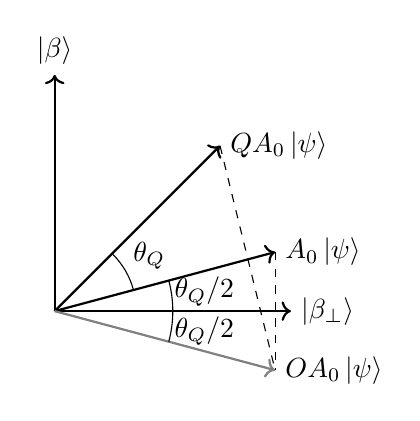
\begin{tikzpicture}
                % 绘制箭头
                \draw[->, thick] (0,0) -- (0,3) node[anchor=south] {$\ket{\beta}$};
                \draw[->, thick] (0,0) -- (2.1,2.1) node[anchor=west] {$QA_{0}\ket{\psi}$};
                \draw[->, thick] (0,0) -- (2.8,0.75) node[anchor=west] {$A_{0}\ket{\psi}$};
                \draw[->, thick] (0,0) -- (3,0) node[anchor=west] {$\ket{\beta_{\perp}}$};
                \draw[->, gray, thick] (0,0) -- (2.8,-0.75) node[anchor=west,black] {$OA_{0}\ket{\psi}$};
                % 绘制虚线
                \draw[dashed] (2.8,0.75) -- (2.8,-0.75);
                \draw[dashed] (2.1,2.1) -- (2.8,-0.75);
                % 绘制角度标记
                \draw (1.5,0) arc[start angle=0,end angle=15,radius=1.5];
                \draw (1.5,0) arc[start angle=0,end angle=-15,radius=1.5];
                \draw (1,0.27) arc[start angle=15,end angle=45,radius=1];
                % 标记角度
                \node at (1.9,0.25) {$\theta_{Q}/2$};
                \node at (1.9,-0.25) {$\theta_{Q}/2$};
                \node at (1.2,0.7) {$\theta_{Q}$};
            \end{tikzpicture}
            \caption{}
            \label{fig:Abdulrahman}
        \end{figure}
        \column{0.6\textwidth}
        和经典Grover类似,对$A_{0}\ket{\psi}$应用
        \begin{equation}
            R_{Q}=\left\lfloor\frac{\pi-\theta_{Q}/2}{\theta_{Q}}\right\rceil
        \end{equation}
        次操作$Q$,有
        \begin{equation*}
            \begin{split}
                Q^{R_{Q}}A_{0}\ket{\psi}= & \cos(\frac{2R_{Q}+1}{2}\theta_{Q})\ket{\beta_{\perp}}             \\
                                          & +\sin(\frac{2R_{Q}+1}{2}\theta_{Q})\ket{\beta}\approx\ket{\beta}.
            \end{split}
        \end{equation*}
    \end{columns}
\end{frame}

\begin{frame}{性能}
    可以看到与经典的迭代次数的比
    \begin{equation}
        R_{Q}/R\approx\theta_{G}/\theta_{Q}\approx 1/\sqrt{2}
    \end{equation}
    这似乎违反了我们曾算过的下界。\\~\\

    可以计算的是,如果目标元素的最后一位是1,有$A_{0}=A(\pi/2)$和$A=A(\pi)$,所以必须要先辨别结果的最后一位,我们才能有效的迭代,这就是加速的来源。
\end{frame}

\begin{frame}{结果}
    \begin{figure}[htbp]
        \centering
        \begin{minipage}[t]{0.48\textwidth}
            \centering
            \includegraphics[scale=0.37]{pic/normal.png}
            \caption{目标态0结尾}
        \end{minipage}
        \begin{minipage}[t]{0.48\textwidth}
            \centering
            \includegraphics[scale=0.37]{pic/unnormal.png}
            \caption{目标态1结尾}
        \end{minipage}
    \end{figure}
\end{frame}

\section*{结语}

\begin{frame}
    \begin{center}
        {\Huge\calligra Best Wishes!}
    \end{center}
\end{frame}



\end{document}